%"Computer Science is no more about computers than astronomy is about telescopes." ~ Edsger Dijkstra
%
% Exemplo LaTeX de monografia UNISINOS
%
% Elaborado com base nas orientações dadas no documento
% ``GUIA PARA ELABORAÇÃO DE TRABALHOS ACADÊMICOS''
% disponível no site da biblioteca da Unisinos.
% http://www.unisinos.br/biblioteca
%
% Os elementos textuais abaixo são apresentados na ordem em que devem
% aparecer no documento.  Repare que nem todos são obrigatórios - isso
% é devidamente indicado em cada caso.
%
% Comentários abaixo colocados entre aspas (`` '') foram
% extraídos diretamente do documento da biblioteca.
%
% Este documento é de domínio público.
%



%TODO: reunião 04/01/19
%	definições (na sec. 4.5) mover para 'decisões de projeto e premissas' e chamar de premissas
%	mover a formula 4.3 pra metodologia?
%	seção 4.3 botar a figura explodida do jmodel + figura explodida do helastic (ver resposta daqui do email)





%=======================================================================
% Declarações iniciais identificando a classe de documento e
% selecionando alguns pacotes adicionais.
%
% As opções disponíveis (separe-as com vírgulas, sem espaço) são:
% - twoside: Formata o documento para impressão frente-e-verso
%   (o default é somente-frente)
% - english,brazilian,french,german,etc.: idiomas usados no documento.
%   Deve ser colocado por último o idioma principal.
%=======================================================================
%TODO: escolher o DocumentClass
%\documentclass[twoside,english,brazilian]{UNISINOSmonografia} % FOR PRINT
\documentclass[english,brazilian]{UNISINOSmonografia} % FOR ONLINE

% place this immediately after the \documentclass line to ensure that all fonts are checked for appropriate resources.
\usepackage{cmap} % melhorar a busca e seleção de texto no pdf

\usepackage[pass]{geometry}

\usepackage[utf8]{inputenc} % charset do texto (utf8, latin1, etc.)
\usepackage[T1]{fontenc} % encoding da fonte (afeta a sep. de sílabas)
\usepackage{microtype} % refinements towards typographical perfection

\usepackage{graphicx} % comandos para gráficos e inclusão de figuras

\usepackage[section]{placeins} %forçar imagens a aparecer depois da própria section
%\usepackage{chronology} % timeline
\RequirePackage{chronoaubin}

%\usepackage[sort]{natbib} % já carregado pelo .cls
\usepackage{bibentry} % para inserir refs. bib. no meio do texto
%\usepackage{usebib} % capturar o título - load after hyperref

\usepackage{paralist} % listas inline

\usepackage{booktabs} % horizontal lines in tables
\usepackage{arydshln} %dashed lines
\usepackage{longtable}
\usepackage{multirow} % multirow in tables
\usepackage{tabularx}  % tabelas melhoradas TODA LARGURA
\usepackage{tabulary}  % tabelas melhoradas MÍNIMA LARGURA
\usepackage{tabu}

\usepackage{pdflscape} % landscape pages
\usepackage{afterpage} % afterpage pra usar no landscape

\usepackage{mathtools}
\usepackage{amsmath}
\usepackage{wasysym}
\usepackage{eurosym}


\usepackage{enumitem}

\usepackage{color, xcolor, colortbl}

%hidelinks
\usepackage{xurl}
\usepackage[breaklinks]{hyperref}


%\usepackage[strict]{changepage}


\graphicspath{{./figs/}}
%\bibinput{Mestrado-clean}
%\citeindextrue

%figuras não ocupam a largura total da página
\newcommand\defaultFigureWidth{0.9}

% espaçamento vertical das tabelas
\renewcommand{\arraystretch}{1.3}

% rotação dos headers de tabelas
\newcommand\tabelaAngulo{90}

% tabularx Centered column
% Y - CENTER
% Z - LEFT
% W - RIGHT
\newcolumntype{Z}{>{\raggedright\arraybackslash}X}
\newcolumntype{Y}{>{\centering\arraybackslash}X}
\newcolumntype{W}{>{\raggedleft\arraybackslash}X}

%chemistry for Helium
\newcommand*\chem[1]{\ensuremath{\mathrm{#1}}}

% Let's us use € to get the \EUR command from the eurosym package.
\DeclareUnicodeCharacter{20AC}{\EUR}



% {arydshln} dashed lines

% \dashedline			- https://tex.stackexchange.com/a/439963
\newcommand{\dashedline}[1]{\noalign{\vskip\aboverulesep}\cdashline{#1}[1pt/4pt]\noalign{\vskip\belowrulesep}}

% cdashlinelr			- https://tex.stackexchange.com/a/320147
\makeatletter
\def\adl@drawiv#1#2#3{%
	\hskip.5\tabcolsep
	\xleaders#3{#2.5\@tempdimb #1{1}#2.5\@tempdimb}%
	#2\z@ plus1fil minus1fil\relax
	\hskip.5\tabcolsep}
\newcommand{\cdashlinelr}[1]{%
	\noalign{\vskip\aboverulesep
		\global\let\@dashdrawstore\adl@draw
		\global\let\adl@draw\adl@drawiv}
	\cdashline{#1}
	\noalign{\global\let\adl@draw\@dashdrawstore
		\vskip\belowrulesep}}
\makeatother



%%%%%%%%
%	BASE COLORS
%%%%%%%%

\definecolor{success-green}{HTML}{009901}%
\definecolor{failure-red}{HTML}{9A0000}%


%=======================================================================
% Escolha do sistema para geração de referências bibliográficas.
%
% O default é usar o estilo unisinos.bst.  Comente a definição abaixo
% e descomente a linha seguinte para usar o estilo do ABNTeX (é
% necessário ter esse pacote instalado).
%
% A vantagem do unisinos.bst é que ele permite o uso de um arquivo .bib
% seguindo as orientações tradicionais do BibTeX (veja essas orientações
% em http://ctan.tug.org/tex-archive/biblio/bibtex/contrib/doc/btxdoc.pdf).
% Entretanto, o estilo não suporta algumas citações mais exóticas como
% apud.  Para isso, use o ABNTeX, mas esteja ciente de que muitas de
% suas referências serão incompatíveis com os estilos tradicionais do
% BibTeX como plain, alpha, ieeetr, entre outros.
%=======================================================================
\unisinosbst
\nobibliography* % para usar o \bibentry
%\usepackage[alf]{abntcite}

%=======================================================================
% Dados gerais sobre o trabalho.
%=======================================================================
\autor{Aubin}{Mateus Rauback}
\titulo{\textsf{H\MakeLowercase{e}}--lastic}
\subtitulo{
	um Modelo de Elasticidade em Nuvem Baseado em Duas Camadas para Acelerar o Cálculo de \textit{best--fit} em Sistemas de Substituição Filogenética}
\orientador[Prof.~Dr.]{Righi}{Rodrigo da Rosa}
\local{São Leopoldo}
\ano{2019}

%% dados específicos para Dissertação de Mestrado
\unidade{Unidade Acadêmica de Pesquisa e Pós-Graduação}
\curso{Programa de Pós-Graduação em Computação Aplicada}
\nivel{Nível Mestrado}
\natureza{%
Dissertação apresentada como requisito parcial para a obtenção
do título de Mestre pelo Programa de Pós-Graduação em Computação
Aplicada da Universidade do Vale do Rio dos Sinos --- UNISINOS
}
%% dados da ficha catalográfica (obrigatória somente para diss. e tese)
%TODO: ficha catalográfica
%004.272.2 Técnicas de processamento paralelo
%004.272.3 Projeto arquitetônico para processamento paralelo
%004.75 Sistemas de processamento distribuído
\cip{Dissertação (mestrado)}{004.75}
\bibliotecario{Bibliotecária responsável: Fulana da Silva}{12/3456}


% cada palavra-chave deve ser fornecida duas vezes, uma em português e
% outra no idioma estrangeiro (na verdade, em tantos idiomas quantos se
% desejar).
\palavrachave{brazilian}{Computação Paralela e Distribuída}
\palavrachave{brazilian}{Computação em Nuvem}
\palavrachave{brazilian}{Elasticidade}
\palavrachave{brazilian}{Bioinformática}
\palavrachave{brazilian}{Filogenética}
\palavrachave{english}{Parallel and Distributed Computing}
\palavrachave{english}{Cloud Computing}
\palavrachave{english}{Elasticity}
\palavrachave{english}{Bioinformatics}
\palavrachave{english}{Phylogenetics}


\hypersetup{
	pdfauthor	= {Mateus R. Aubin},
	pdftitle	= {He-lastic: um Modelo de Elasticidade em Nuvem Baseado em Duas Camadas para Acelerar o Cálculo de best-fit em Sistemas de Substituição Filogenética},
	pdfsubject	= {Dissertação apresentada como requisito parcial para a obtenção do título de Mestre pelo Programa de Pós-Graduação em Computação Aplicada UNISINOS},
	pdfkeywords	= {Parallel and Distributed Computing} {Cloud Computing} {Elasticity} {Bioinformatics} {Phylogenetics} {Computação Paralela e Distribuída} {Computação em Nuvem} {Elasticidade} {Bioinformática} {Filogenética},
	breaklinks	= true,
	unicode		= true, % non-Latin characters in Acrobat’s bookmarks
	linktoc		= all,
	pdflang		= pt-BR,
	colorlinks=true,
	allcolors=[RGB]{0,0,100}
}
\AtBeginDocument{\colorlet{defaultcolor}{.}}


%=======================================================================
% Início do documento.
%=======================================================================
\begin{document}
%\usebibentry{bib-key}{field}


\capa
\folhaderosto
\folhadeaprovacao % não deve ser incluída nos TCCs

%=======================================================================
% Dedicatória (opcional).
%
% O texto é normalmente colocado na parte de baixo da página, alinhado
% à direita.  Mas a formatação é basicamente livre.  Só não se escreve
% a palavra 'dedicatória'.
%=======================================================================
%\begin{dedicatoria}
%Aos nossos pais.\\[4ex] % quebra a linha dando um espaçamento maior
%\begin{itshape} % faz o texto ficar em itálico
%If I have seen farther than others,\\
%it is because I stood on the shoulders of giants.\\
%\end{itshape}
%--- \textsc{Sir Isaac Newton} % \textsc é o "small caps"
%\end{dedicatoria}

%=======================================================================
% Agradecimentos (opcional).
%=======================================================================
\begin{agradecimentos}
	
	Ao Prof.~Dr. Rodrigo da Rosa \textbf{Righi} pelo tempo e a confiança continuamente investidos em mim desde a graduação.
	\\[1ex]
	
	A minha noiva, \textbf{Natália}, por me dar condições para desenvolver este trabalho e me apoiar incondicionalmente.
	\\[1ex]
	
	Aos meus \textbf{pais} que sempre me incentivaram a buscar e aprimorar meus conhecimentos.
	\\[1ex]
	
	Aos demais \textbf{professores} que influenciaram na minha trajetória desde a Graduação até aqui no Mestrado, em especial aos professores Cristiano André da Costa e Jorge Luis Victória Barbosa pelas contribuições durante o desenvolvimento desta dissertação.
	\\[1ex]
	
	A Coordenação de Aperfeiçoamento de Pessoal de Nível Superior (\textbf{CAPES}), pela bolsa de estudos.
	\\[1ex]

	A Fundação de Amparo à Pesquisa do Estado do Rio Grande do Sul (\textbf{FAPERGS}), por contemplar nossa proposta, Combinando Elasticidade Multi-Métrica em Nuvem nas Modalidades Vertical e Horizontal para Análise de Genes e Redução de Pragas Agrícolas, no Edital 02/2017 - PqG.

\end{agradecimentos}

%=======================================================================
% Epígrafe (opcional).
%
% ``[...] o autor apresenta uma citação, seguida de indicação de autoria,
% relacionada com a matéria tratada no corpo do trabalho. Podem, também,
% constar epígrafes nas folhas de aberturas das seções primárias.''
%=======================================================================
%\begin{epigrafe}
%``\textit{Ninguém abre um livro sem que aprenda alguma coisa}''.\\
%(Anônimo)
%\end{epigrafe}


%=======================================================================
% Resumo em Português.
%
% A recomendação é para 150 a 500 palavras.
%=======================================================================
\begin{abstract}

%TODO: Valorizar a análise de custo benefício \autoref{sec:modelo-custben}
%taxonomia

% == problema & motivação
Atualmente são escassos os exemplos de áreas do conhecimento que não se beneficiam de recursos tecnológicos para aumentar a produtividade .
Também figurando como uma das beneficiadas por esta tendência, a bioinformática, que surge da união entre biologia, ciência da computação e medicina, estabeleceu técnicas, algoritmos e bases de dados que se tornaram fundamentais para o execício da pesquisa, seja no âmbito acadêmico ou profissional.
Avanços recentes como as tecnologias de Sequenciamento genético de Próxima Geração (NGS) trouxeram abundância de dados para a bioinformática e a filogenética, que foca no estudo das relações genealógicas entre organismos, aumentando a qualidade dos estudos outrora limitados apenas a observações manuais.
% == objetivos
Com o objetivo de aumentar o conhecimento sobre bioinformática e filogenética, de especial relevância para o projeto contemplado pela FAPERGS em colaboração com o laboratório de Biologia da UNISINOS, buscamos realizar um mapeamento do estado da arte através de uma revisão da literatura que contribuiu para a elaboração de uma taxonomia capaz de classificar os projetos de software encontrados em termos de suas categorias, métodos e finalidades.
Concluímos com base na bibliografia que, contrastando com os recentes avanços na filogenética, os projetos de software estão tecnologicamente defasados, demandando investimentos em modernização principalmente no que diz respeito a aplicação de técnicas mais recentes como elasticidade de recursos, balanceamento de carga e aceleração por GPUs.
Nossa principal contribuição se dá através do modelo \textsf{He}--lastic onde propomos uma abordagem de otimização para o projeto jModelTest que contempla o uso de elasticidade de recursos em um ambiente de computação em nuvem, resultando em uma arquitetura de elasticidade em duas camadas, baseada nas tecnologias de FaaS e Orquestração de Contêineres e que tem por objetivo absorver, na primeira camada, as tarefas de curta duração, deixando as demais para a segunda camada de elasticidade.
%todo: resultados
% == futuro
Seguindo adiante buscamos futuramente aprimorar a taxonomia e, principalmente, implementar o modelo proposto através de um protótipo, utilizando-o na avaliação dos cenários propostos neste trabalho e objetivando uma análise comparativa com o estado atual do projeto jModelTest sob a luz de critérios como a eficiência computacional e econômica da nossa proposta.


\end{abstract}

%=======================================================================
% Resumo em língua estrangeira (obrigatório somente para teses e
% dissertações).
%
% O idioma usado aqui deve necessariamente aparecer nos parâmetros do
% \documentclass, no início do documento.
%=======================================================================
\begin{otherlanguage}{english}
\begin{abstract}
	
Currently there are few examples of areas of knowledge that do not benefit from technological resources to increase productivity.
Also one of the beneficiaries of this trend, bioinformatics, which emerges from the combination of knowledge in biology, computer science and medicine, has established techniques, algorithms and databases that have become fundamental for research, whether in the academic or professional spheres.
Recent advances such as Next Generation Sequencing (NGS) technologies have brought abundance of data to bioinformatics and phylogenetics, which focuses on the study of genealogical relationships between organisms, increasing the quality of studies once limited to manual observations.
With the objective of increasing the knowledge about bioinformatics and phylogenetics, of special relevance to the project funded by FAPERGS in collaboration with the Biology laboratory of UNISINOS, we sought to carry out a mapping of the state of the art through a literature review that contributed to the formulation of a taxonomy capable of classifying the software projects found in terms of their categories, methods and purposes.
We conclude, on the basis of the bibliography, that in contrast to the recent advances in phylogenetics, software projects are technologically outdated, requiring investments in modernization mainly regarding the application of more recent techniques such as resource elasticity, load balancing and GPU acceleration .
Our main contribution is through the \textsf{He}--lastic model, where we propose an optimization approach for the jModelTest project that contemplates the use of resource elasticity in a cloud computing environment, resulting in a elasticity architecture composed of two layers based on FaaS and Container Orchestration technologies and that aims to absorb, in the first layer, short duration tasks, leaving the remaining tasks for the second layer of elasticity.
In the future, we intend to improve the taxonomy and, mainly, to implement the proposed model through a prototype, using it in the evaluation of the scenarios proposed in this work and aiming at a comparative analysis with the current state of the jModelTest project under light of criteria such as computational and economic efficiency of our proposal.

\end{abstract}
\end{otherlanguage}

%=======================================================================
% Lista de Figuras (opcional).
%=======================================================================
\begingroup
\hypersetup{linkcolor=defaultcolor}
	\listoffigures
\endgroup

%=======================================================================
% Lista de Tabelas (opcional).
%=======================================================================

\begingroup
\hypersetup{linkcolor=defaultcolor}
	\listoftables
\endgroup

%=======================================================================
% Lista de Abreviaturas (opcional).
%
% Deve ser passada como parâmetro a maior das abreviaturas utilizadas.
%=======================================================================
%\begin{listadeabreviaturas}{seg., segs.}
%\item[ampl.] ampliado, -a
%\item[atual.] atualizado, -a
%\item[coord.] coordenador
%\item[N.~T.] Novo Testamento
%\item[seg., segs.] seguinte, -s
%\end{listadeabreviaturas}

%=======================================================================
% Lista de Siglas (opcional).
%
% Deve ser passada como parâmetro a maior das siglas utilizadas.
%=======================================================================
\begin{listadesiglas}{MMMMM}
	\item[ACM] Associação para Maquinas Computacionais \newline \textit{Association for Computing Machinery}
	\item[AKS] \textit{Azure Kubernetes Service}
	\item[API] Interface de Programação de Aplicação \newline \textit{Application Programming Interface}
	\item[AWS] Amazon Serviços da Web \newline \textit{Amazon Web Services}
	\item[BMC] \textit{BioMed Central}
	\item[BSP] Fases Paralelas \newline \textit{Bulk Synchronous Parallel}
	\item[CAPES] Coordenação de Aperfeiçoamento de Pessoal de Nível Superior
	\item[CPU] Unidade Central de Processamento \newline \textit{Central Processing Unit}
	\item[CV] Coeficiente de Variação \newline \textit{Coefficient of Variation}
	\item[DNA] Ácido Desoxirribonucleico \newline \textit{Deoxyribonucleic Acid}
	\item[EC2] \textit{Elastic Compute Cloud}
	\item[ECS] \textit{Elastic Container Service}
	\item[FAPERGS] Fundação de Amparo à Pesquisa do Estado do Rio Grande do Sul
	\item[FASTA] Fast ALL
	\item[FaaS] Função como Serviço \newline \textit{Function as a Service}
	\item[FaaS] Função como um Serviço \newline \textit{Function as a Service}
	\item[GCP] \textit{Google Cloud Platform}
	\item[GFLOP] Giga Operações de Ponto Flutuante por Segundo \newline \textit{Giga Floating Point Operations per Second}
	\item[GPU] Unidade de Processamento Gráfico \newline \textit{Graphics Processing Unit}
	\item[HGT] Transferência Horizontal de Genes \newline \textit{Horizontal Gene Transfer}
	\item[I/O] Entrada e Saída \newline \textit{Input and/or Output}
	\item[IEEE] Instituto dos Engenheiros Elétricos e Eletrônicos \newline \textit{Institute of Electrical and Electronics Engineers}
	\item[IaaS] Infraestrutura como Serviço \newline \textit{Infrastructure as a Service}
	\item[LBA] Atração por Longas Ramificações \newline \textit{Long Branch Attraction}
	\item[MCMC] Cadeias de Markov Monte Carlo \newline \textit{Markov Chain Monte Carlo}
	\item[ML] Máxima Verossimilhança \newline \textit{Maximum Likelihood}
	\item[MPI] Interface de Passagem de Mensagens \newline \textit{Message Passing Interface}
	\item[MSA] Alinhamento de Múltiplas Sequências [moleculares] \newline \textit{Multiple Sequence Alignment}
	\item[NCBI] Centro Nacional de Informações Biotecnológicas \newline \textit{National Center for Biotechnology Information}
	\item[NGS] Sequenciamento de Próxima Geração \newline \textit{Next Generation Sequencing}
	\item[NIST] Instituto Nacional de Padrões e Tecnologia \newline \textit{National Institute of Standards and Technology}
	\item[PLOS] Biblioteca Pública de Ciências \newline \textit{Public Library of Science}
	\item[PVM] Máquina Virtual Paralela \newline \textit{Parallel Virtual Machine}
	\item[PaaS] Plataforma como Serviço \newline \textit{Platform as a Service}
	\item[RNA] Ácido Ribonucleico \newline \textit{Ribonucleic Acid}
	\item[UML] Linguagem Unificada de Modelagem \newline \textit{Unified Modelling Language}
	\item[UNISINOS] Universidade do Vale do Rio dos Sinos
	\item[VM] Máquina Virtual \newline \textit{Virtual Machine}
	%\item[BEAGLE] Broad-platform Evolutionary Analysis General Likelihood Evaluator
	%\item[BEAST] Bayesian Evolutionary Analysis Sampling Trees \newline Análise Evolucionária Bayesiana por Amostragem de Árvores
	%\item[BLAST] Basic Local Alignment Search Tool
	%\item[CAPES] Coordenação de Aperfeiçoamento de Pessoal de Nível Superior
	%\item[FAPERGS] Fundação de Amparo à Pesquisa do Estado do Rio Grande do Sul
	%\item[MEGA] Molecular Evolutionary Genetics Analysis \newline Análise Genética Molecular Evolucionária
	%\item[MUSCLE] MUltiple Sequence Comparison by Log-Expectation
	%\item[NCBI] National Center for Biotechnology Information \newline Centro Nacional de Informações Biotecnológicas
	%\item[SIMD] Single Instruction Multiple Data
	%\item[XML] Extensible Markup Language
\end{listadesiglas}

%=======================================================================
% Lista de Símbolos (opcional).
%
% Deve ser passado o maior (mais largo) dos símbolos utilizados.
%=======================================================================
%\begin{listadesimbolos}{Ca}
%\item[\textsuperscript{o}C] Graus Celsius
%\item[Al] Alumínio
%\item[Ca] Cálcio
%\end{listadesimbolos}

%=======================================================================
% Sumário
%=======================================================================

\begingroup
\hypersetup{linkcolor=defaultcolor}
	\tableofcontents
\endgroup

%=======================================================================
% Introdução
%=======================================================================
\chapter{Introdução}
\label{ch:intro}

% as epígrafes nos capítulos são opcionais
\epigrafecap{You must not come lightly to the blank page.}{Stephen King}


A biologia, no seu estudo dos seres vivos, é uma das mais antigas faces da ciência e por isso diversas foram as mudanças em seus modos de pesquisa ao longo dos anos.
Eventualmente equipamentos de informática passaram a dividir espaço com microscópios nos laboratórios, aliando novas tecnologias ao vasto conhecimento acumulado em busca de respostas sobre as origens e os mecanismos de funcionamento da vida.


Atualmente são escassos os exemplos de áreas do conhecimento que não se beneficiam de recursos tecnológicos para aumentar a produtividade \cite{Denning2009}.
Não é diferente com a biologia que, através da união de esforços com a medicina e a informática criou uma área específica de estudo, a bioinformática.
Através desta colaboração surgiram algoritmos e bases de dados que se mostram, hoje em dia, fundamentais para o exercício da pesquisa, seja ela acadêmica ou profissional \cite{NCBI-Handbook}.
Projetos como o de mapeamento do genoma humano \cite{Venter2001}, inciado em 1990 com o apoio de múltiplos países, impulsionaram a colaboração entre estas áreas, garantindo avanços significativos nos seus respectivos domínios do conhecimento.


Embora os avanços tenham sido significativos e amplamente variados, o acesso crescente a tecnologias como as de mapeamento genético aumentou o volume de dados gerado a partir de estudos biológicos, antes limitados a observações manuais \cite{book:2119998}.
Bancos de dados de amostras genéticas, como o NCBI\footnote{
	Acessível através da URL: \url{https://www.ncbi.nlm.nih.gov/}
} \cite{NCBI-Handbook}, guardam uma infinidade de indivíduos das mais variadas espécies, possibilitando que pesquisadores realizem estudos tão amplos quanto aqueles que buscam mapear a árvore da vida, ou tão especializados quanto aqueles que se focam no estudo de uma única doença, por exemplo.

%aqui!


Além disso, mudanças nas arquiteturas de computadores e sistemas invalidaram diversas das hipóteses sobre as quais se apoiavam algumas das mais antigas soluções.
Dentre as alterações mais emblemáticas estão a evolução dos processadores através do paralelismo, abandonando a corrida pelas cada vez maiores frequências de \textit{clock} \cite{Baker1999}, e o surgimento da computação em nuvem, que muda completamente a economia de escala e a necessidade de se comprar e manter recursos computacionais frente a oferta de computação virtualmente infinita pelos provedores \cite{NIST}.


Chegamos, então, a um ponto onde se faz necessária uma intervenção nos algoritmos e programas de bioinformática visando readequá-los a este novo cenário baseado em grandes volumes de dados e na computação em nuvem.
Para tanto o presente trabalho se propõe a realizar uma análise no cenário tecnológico no que tange aos processos e métodos de análise e inferência filogenética.
Mais do que isso, a intenção é gerar ganhos que possam se estender a toda a comunidade acadêmica por meio de um modelo de computacional baseado em elasticidade de duas camadas.



\section{Motivação}


%def> filogenetica e bioinformatica
% 	> disponibilidade de dados genéticos

Resultado da poderosa combinação entre biologia, medicina e tecnologia da informação, a bioinformática se apresenta como um campo de estudo interdisciplinar focado em desvendar os mistérios da vida.
Uma de suas vertentes, a filogenética (\autoref{sec:bioinformatica}), estreita o foco de pesquisa para a compreensão da evolução dos organismos e suas relações ancestrais através do uso de conhecimentos da genética e da genômica, combinados com estudos da teoria evolutiva.
O advento das tecnologias chamadas de NGS, (\textit{Next Generation Sequencing}) reduziu barreiras para a obtenção de sequências genéticas, ampliando a disponibilidade de dados genéticos e contribuindo para o objetivo definitivo da filogenética \cite{book:2119998,yang2014molecular}, encontrar o ancestral universal a todos os organismos vivos.


%	> atraso na computação e elasticidade

Apesar dos avanços no que diz respeito a obtenção de material genético, quando tratando-se de aspectos computacionais foi identificada, através de um extensivo levantamento bibliográfico (\autoref{sec:analise-estadodaarte}), uma lacuna tecnológica que se torna evidente quando investigamos na intersecção entre filogenética e técnicas computacionais como computação distribuída, aceleração por GPU, o uso de elasticidade de recursos e técnicas de balanceamento de carga.
Especulamos que tal situação tenha advindo do fato de que os algoritmos e métodos da filogenética são considerados maduros e bem definidos, enquanto as técnicas computacionais mencionadas se popularizaram anos depois.
Esta situação é especialmente notória no que diz respeito ao uso de computação em nuvem e, mais especificamente, na elasticidade de recursos.
\citetexto{Jonas2017} corroboram com esta hipótese ao postular que grande parte dos projetos de software para aplicações científicas e de análise não foi escrito por cientistas da computação e que este grupo foi deixado de fora da revolução que se tornou a computação em nuvem.


%	> projeto da biologia

Através da oportunidade de colaboração com o laboratório de biologia da UNISINOS por meio do projeto contemplado pela FAPERGS -- ``Combinando Elasticidade Multi-Métrica em Nuvem nas Modalidades Vertical e Horizontal para Análise de Genes e Redução de Pragas Agrícolas'', o objetivo do presente trabalho é dar um significativo passo também rumo aos objetivos desta iniciativa, realizando um reconhecimento do estado da arte e estabelecendo as lacunas de pesquisa mais evidentes no contexto do projeto.
Com a intenção de fomentar um entendimento compartilhado entre os colaboradores do projeto busca-se estabelecer, também, uma taxonomia referente à classificação dos objetivos dos trabalhos encontrados no estado da arte.
Assim temos, nesta proposta, um dos primeiros resultados em relação a esta colaboração, aplicando conhecimentos de computação de alto desempenho, através da elasticidade oriunda da computação em nuvem, com o propósito de mitigar as dificuldades encontradas por pesquisadores que atuam na filogenética.



%	> possibilidade de aumentar a qualidade da produção cientifica

Ao mapear os pontos de melhoria e propor novas abordagens para as ferramentas utilizadas no contexto de filogenética torna-se possível acelerar o processamento de dados e a quantidade de amostras sob análise, aumentando não só a eficiência dos programas como também dos profissionais da bioinformática.
Dentre os benefícios esperados com esta abordagem é possível citar, em primeiro lugar, o aumento no uso de análises que talvez não sejam feitas em função da sua complexidade computacional e tempo de execução proibitivo e, em segundo lugar, a redução no tempo gasto pelos pesquisadores que já utilizam tais processos e ferramentas, possibilitando seu investimento na análise dos resultados obtidos.
Em última instância estes fatores combinados têm potencial para contribuir em termos de qualidade e profundidade das análises no âmbito da filogenética, avançando a produção científica.



\section{Questão de Pesquisa} %modelo... o que te move?!


Instigado pelos motivos citados embarcamos nesta jornada buscando aplicar nossos conhecimentos no campo da elasticidade pela computação em nuvem aos projetos da filogenética, definindo do seguinte modo nossa questão de pesquisa:


\begin{quote}
	\large
	como seria \textbf{projetado um modelo} de \textbf{elasticidade} de recursos em um ambiente de computação em nuvem capaz de aperfeiçoar o processo de \textbf{adequação de sistemas} de substituição de sequências moleculares da \textbf{filogenética} de maneira \textbf{eficiente} do ponto de vista \textbf{computacional e econômico}?
	
% 	``Quais são, no âmbito da \textbf{filogenética}, os projetos \textbf{candidatos} a atualização tecnológica através da implementação de \textbf{elasticidade} em um contexto de computação em nuvem e como \textbf{projetar um modelo} capaz de preencher esta lacuna de maneira \textbf{eficiente} do ponto de vista \textbf{computacional e econômico}?''
\end{quote}


Para viabilizar a resposta à esta pergunta se torna necessário esclarecer os elementos destacados na questão de pesquisa e que são detalhados ao longo deste documento nos seguintes pontos:

\begin{itemize}
	
	\item \textbf{Projeto de um Modelo:} a partir da definição de um conjunto de decisões sobre o projeto (\autoref{sec:modelo-decisoes}) foi possível elaborar e detalhar a arquitetura de um modelo computacional (\autoref{sec:modelo-arquitetura}) capaz de endereçar a presente questão de pesquisa;
	
	\item \textbf{Elasticidade:} apresentada por meio da fundamentação teórica na \autoref{sec:computacao};
	
	\item \textbf{Adequação de Sistemas:} através de uma análise comparativa (\autoref{sec:analise-estadodaarte}) foi encontrada uma quantidade significativa de projetos e delineamos as lacunas de pesquisa (\autoref{sec:lacunas-de-pesquisa}) para, finalmente, escolher uma aplicação candidata para o desenvolvimento (\autoref{sec:modelo-selecao});
	
	\item \textbf{Filogenética:} também apresentada por meio da fundamentação teórica na \autoref{sec:bioinformatica};
	
	\item \textbf{Eficiente Computacional e Economicamente:} através do detalhamento das estratégias de elasticidade (\autoref{sec:estrategias-elasticidade}) foi formulada uma metodologia de avaliação (\autoref{ch:modelo-metodologia}) que será fundamental para estabelecer a eficiência de nossa proposta.
\end{itemize}



\section{Objetivos}
\label{sec:objetivos}

%O objetivo geral para esse trabalho é propor um modelo computacional para a triagem, monitoramento de pacientes e alerta precoce que visa apoiar a equipe de saúde e interagir com os pacientes do departamento de emergência de hospitais, utilizando os protocolos de deterioração de sinais vitais em conjunto com os protocolos de triagem.


Conhecendo as motivações e a questão de pesquisa no âmbito deste trabalho, podemos estabelecer que seu objetivo geral é:
\begin{quote}
	\large
	propor um modelo computacional que empregue a elasticidade de recursos oriunda da computação em nuvem para aumentar a eficiência computacional e econômica no problema do teste de adequação de sistemas de substituição de sequências moleculares no contexto da filogenética.
\end{quote}
Contudo, visando detalhar este objetivo, assim como seus requisitos e resultados esperados, devemos dividi-lo em termos dos seus componentes, ou seja, os objetivos específicos desta pesquisa, sendo eles:


\begin{enumerate}[label=Objetivo~\arabic*:~,itemindent=*]
	
	\item Familiarizar-se com a bioinformática e mais especificamente a filogenética;
	
	\item Mapear o estado da arte no que diz respeito aos softwares utilizados no âmbito da filogenética;
	
	\item Estabelecer uma taxonomia para classificação destes projetos e as características relevantes do ponto de vista computacional para identificar candidatos à receber as melhorias propostas;
	
	\item Projetar um modelo capaz de fornecer ao projeto candidato capacidades de elasticidade de recursos com vistas a torná-lo apto para uso em ambientes de computação em nuvem;
	
	\item Estabelecer uma arquitetura e estratégias capazes de, através da elasticidade, obter ganhos de performance, aproveitamento de recursos e redução no fardo operacional, resultando em decréscimo no custo de operação do software;
	
	\item Avaliar, através de análises comparativas, o quão eficaz será nosso modelo frente ao projeto candidato na sua forma atual.
	
\end{enumerate}


%Através desses objetivos individuais, espera-se obter um modelo que resulte na amenização
%do maior problema das F-RANs: o acesso excessivo ao fronthaul, o qual é um componente centralizado. Como consequência, espera-se que o modelo proposto reduza a latência de rede em horários de pico.

\section{Estrutura do Texto}


O restante do texto está estruturado da seguinte forma: no \autoref{ch:fundamentacao} é apresentada a base teórica que sustenta esta pesquisa, composta majoritariamente por conhecimentos das áreas da Bioinformática e da Computação de Alto Desempenho. 
Dentre estes domínios são de especial interesse para esta dissertação os métodos de Inferência Filogenética e a Computação em Nuvem, mais especificamente o conceito de Elasticidade.

No \autoref{ch:relacionados} apresentam-se os trabalhos relacionados, assim como os critérios de seleção e escolha da literatura científica que contribuíram para determinar o estado da arte no que tange os assuntos abordados neste trabalho.
Uma análise comparativa auxilia o leitor a compreender o panorama da área de estudo e contribui para a identificação de possíveis lacunas de pesquisa, onde esta dissertação se insere e busca, através do modelo proposto, sua contribuição científica.


Em seguida, no \autoref{ch:modelo}, o leitor será apresentado ao modelo \textsf{He}--lastic, sendo esta uma estratégia para preencher algumas das lacunas de pesquisa previamente identificadas. Aborda-se neste capítulo as questões relacionadas à decisões de projeto, arquitetura estratégias de elasticidade e as métricas de avaliação para o modelo proposto, fornecendo um panorama conceitual da solução apresentada


No \autoref{ch:modelo-metodologia} é apresentada a metodologia de avaliação do modelo proposto, abordando as etapas e os cenários que fazem parte da avaliação, aproveitando, também, para descrever em maiores detalhes as questões práticas da avaliação, abordando características da aplicação, da infraestrutura utilizada, assim como o desenvolvimento do protótipo e seus parâmetros.


A seguir, no \autoref{ch:resultados}, são apresentados os resultados obtidos conforme o protocolo de avaliação previamente descrito, onde são abordadas questões que dizem respeito a análise de custo--benefício da estratégia de elasticidade adotada pelo modelo proposto, os resultados da avaliação da aplicação de referência, e os resultados da avaliação do modelo \textsf{He}--lastic em suas variações, reservando também espaço para discussão sobre a comparação em termos de custo financeiro entre as duas abordagens.


Enfim, no \autoref{ch:conclusao}, encerra-se a pesquisa com a apresentação das principais contribuições oriundas da adoção do modelo proposto, assim como, os possíveis caminhos disponíveis para aprofundar e aperfeiçoar a proposta desta dissertação em trabalhos futuros.


%=======================================================================
% Fundamentação Teórica
%=======================================================================
\chapter{Fundamentação Teórica}
\label{ch:fundamentacao}


% as epígrafes nos capítulos são opcionais
\epigrafecap{Knowledge speaks, but wisdom listens.}{Jimi Hendrix}


Este capítulo apresenta conceitos fundamentais para o completo entendimento do presente trabalho, assim como, conceitos básicos das áreas de estudo e referências adicionais.
Sendo imprescindíveis para a apreciação deste trabalho, conhecimentos nas áreas de bioinformática, filogenética e computação de alto desempenho.



Em um primeiro momento serão abordadas questões como:
\begin{inparaenum}[\itshape a\upshape)] 
	\item o que são sequências moleculares;
	\item como funciona o processo de inferência filogenética;
	\item quais são os métodos utilizados para este fim; e
	\item como modelos matemáticos são usados para auxiliar este processo.
\end{inparaenum}
A seguir, apresentam-se questões relevantes ao domínio da ciência da computação, mais especificamente, no que diz respeito à computação de alto desempenho e alguns dos seus facilitadores como:
\begin{inparaenum}[\itshape a\upshape)] 
	\item técnicas de computação paralela e distribuída;
	\item estratégias de decomposição de problemas;
	\item o surgimento da computação em nuvem e suas implicações;
	\item o conceito de elasticidade de recursos e sua importância;
	\item o emprego de orquestração de contêineres como facilitador da elasticidade; e
	\item a ascensão das plataformas de \textit{Function as a Service} (FaaS).
\end{inparaenum}


\section{Bioinformática e Filogenética}
\label{sec:bioinformatica}


A bioinformática pode ser definida, segundo \citetexto{NCBI-Handbook}, como uma abordagem computacional para a gestão de conhecimento e análise de dados biomédicos, ou seja, um campo de estudo multidisciplinar que une os conhecimentos das áreas de biologia, medicina e tecnologia da informação.
Tal combinação mostra-se relevante diante da crescente capacidade computacional e do volume de dados disponíveis para análises, auxiliando acadêmicos da biologia e da medicina na expansão do conhecimento científico.
Uma definição ainda mais detalhada pode ser encontrada em \citetexto{Moore2007}, ao afirmar que o objetivo da bioinformática é ``facilitar a gestão, análise e interpretação de dados oriundos de observação e experimentos, contemplando o desenvolvimento e a implementação de bancos de dados, análise de dados, mineração de dados e a interpretação e inferência de dados biológicos''.


%[Keane2006a]
%The Origin of Species by Means of Natural Selection, or
%The Preservation of Favoured Races in the Struggle for Life (Darwin, 1859).
%In this book he proposed that ‘all the organic beings which have ever lived on
%this earth have descended from some one primordial form’.
%
%This led to the creation of a new area of science whose
%goal has been the study of evolutionary history of all organisms. Darwin
%provided scientists with a general framework on how to infer relationships
%among species using morphological, paleontological, and biogeographical in-formation.
%
%Although Darwin understood and was able to explain the process of natural
%selection, he did not fully understand how it operates principally because
%the genetic basis for inheritance was not known at the time. Mendel was
%the first to reveal the secrets of how heredity and variability in populations
%worked (Mendel, 1866). However it was not until the 20th century with
%the publication of the synthetic theory of evolution (neo-Darwinism) did
%the fields of genetics and evolution unite (Huxley, 1974). It was recognised
%that genetic mutation is the essential ingredient that introduces the variation
%required for natural selection to work.


Assim como a bioinformática, que advém da combinação entre biologia e ciência da computação, a filogenética emerge da associação entre os conhecimentos em biologia evolutiva e, mais recentemente, da genética.
\citetexto{darwin1859} delineou as fundações da teoria evolutiva e toda uma área de estudo, em sua obra ``A Origem das Espécies'', além de postular que todas as formas de vida na Terra descendem de um ancestral primordial.
Neste contexto, Darwin equipou cientistas com um \textit{framework} para inferência de relacionamentos entre espécies a partir de informações morfológicas, paleontológicas e biogeográficas \cite{Keane2006a}.
Posteriormente, \citetexto{mendel1866}, através do seu artigo ``Experimentos na hibridização de plantas'', introduziu conceitos básicos da genética como hereditariedade (através das características recessivas e dominantes), além da variabilidade de populações, fornecendo a teoria que até hoje suporta a genética como uma área de estudo.


%The universal common ancestor for all living organisms is termed cenancestor which may or may not be identifiable \cite{Xia2014}


%\cite{Adachi1996}
%The objectives of phylogenetic studies are (1)
%to reconstruct the correct genealogical ties between organisms and (2) to estimate the time of divergence
%between organisms since they last shared a common ancestor.


Embora atualmente a relação entre estas duas áreas seja evidente, foi apenas no início do século XX que ambas correntes de pensamento foram unificadas em uma formulação teórica e matemática posteriormente batizada por \citetexto{huxley1974} de neo-Darwinismo.
Avanços tecnológicos e o sequenciamento genético possibilitaram o surgimento da biologia molecular e da genômica (estudos com base no sequenciamento completo de um indivíduo) como áreas de estudo, sendo estas, o elo faltante para a definição da filogenética.
\citetexto{Adachi1996} afirmam que os objetivos de estudos filogenéticos são duplos: de um lado reconstruir a mais correta relação genealógica entre organismos; e de outro, estimar a divergência de tempo desde que tais organismos compartilharam um ancestral comum.
Extrapolando esta definição, \citetexto{Xia2014}, estabelece como derradeiro objetivo da filogenia encontrar o ancestral universal a todos os organismos vivos, denominado \textit{cenancestor}.




\subsection{Alinhamento de Sequências Moleculares}


Por meio do acúmulo de material genético mapeado torna-se evidente o ímpeto de pesquisadores, no verdadeiro espírito Darwiniano, ao comparar múltiplas amostras para identificar similaridades e pontos de diferença.
No entanto, antes que qualquer análise comparativa possa ser realizada, é de suma importância garantir que as amostras sejam análogas entre si, evitando o risco de, em termos simples, comparar bicicletas com bananas.
Neste momento, o alinhamento de sequências se apresenta como solução, uma vez que alinhamentos corretos são úteis para a predição estrutural e funcional de proteínas e, conforme apresentado na \autoref{s:phylogeneticinference}, indispensáveis para a análise filogenética \cite{biofordummies2007}.


%\cite{Zwickl2006b}
%Sequence data are
%composed of a series of characters drawn from a limited alphabet. These characters are
%referred to as bases or nucleotides in the case of DNA (A, C, G and T) and RNA (A, C, G
%and U) sequence, and amino acids in the case of protein sequence (A, C, D, E, F, G, H, I,
%K, L, M, N, P, Q, R, S, T, V, W and Y). The preference for sequence data is primarily
%due to the ease and speed with which many characters can be gathered and the tractability
%of statistically modeling the process of sequence evolution.


Sequências genéticas podem ser representadas como sequências de caracteres oriundas de um alfabeto limitado \cite{DarribaPHD}, podendo ser chamadas de bases ou nucleotídeos no caso de ácido desoxirribonucleico (DNA) e ácido ribonucleico (RNA), ou então de aminoácido no caso das proteínas.
\citetexto{Zwickl2006} explica que a preferência por dados de sequências genéticas se dá primordialmente pela facilidade e a velocidade com que os caracteres podem ser coletados e a tratabilidade no caso de modelagens estatísticas.
Tais sequências costumam ser armazenadas em meios digitais através de formatos de arquivo como FASTA, exemplificado na \autoref{fig:arquivo-fasta}, e NEXUS, por exemplo, empregando representações de DNA, RNA, e aminoácidos, apresentadas respectivamente nas Tabelas \ref{tab:dna-codes}, \ref{tab:rna-codes} e \ref{tab:amino-codes}.


%\cite{book:2119998}
%O
%NE OF THE MOST IMPORTANT CONTRIBUTIONS of molecular biology to evolutionary anal- ysis is the discovery that the DNA sequences of different organisms are often related.
%
%Computationally, msa presents
%several difficult challenges. First, finding an optimal alignment of more than two sequences
%that includes matches, mismatches, and gaps, and that takes into account the degree of
%variation in all of the sequences at the same time poses a very difficult challenge.
%
%A second computational challenge is identifying a
%reasonable method of obtaining a cumulative score for the substitutions in the column of
%an msa. Finally, the placement and scoring of gaps in the various sequences of an msa pre-sents an additional challenge.
%
%Once the msa has been found, the number or types of changes in the aligned sequence
%residues may be used for a phylogenetic analysis.


Computacionalmente, o alinhamento de múltiplas sequências, MSA, apresenta pelo menos três grandes desafios identificados por \citetexto{book:2119998}, sendo eles: \begin{inparaenum}[\itshape a\upshape)] 
	\item encontrar um alinhamento ótimo entre mais de duas sequências que compreenda equivalências, diferenças e lacunas, além de, considerar também, o grau de variação entre todas as sequências;
	\item identificar um método razoável para calcular um critério de pontuação das colunas alinhadas; e
	\item posicionamento e critérios de pontuação das lacunas presentes dentre as várias sequências.
\end{inparaenum}
Somente assim, uma vez alinhadas as sequências, é possível executar uma comparação justa entre as diferentes amostras disponíveis.


%\cite{biofordummies2007}
%We introduce three different multiple-sequence-alignment methods
%that should cover most of your needs: ClustalW because everybody uses it,
%MUSCLE because it is very fast, Tcoffee because it is very accurate, and can
%let you combine sequences and structures.
%
%alignments are useful for predicting
%protein structures (see Chapter 11), central for predicting the function of
%proteins, and indispensable for phylogenetic analysis (see Chapter 13).
%
%ClustalW uses a progressive method to build its alignments. Instead of aligning
%all the sequences at the same time, it adds them one by one.
%
%Tcoffee builds a progressive alignment like ClustalW, but it compares segments
%across the entire sequence set.
%its ability to align sequences and structures (EXPRESSO), the possibility of evaluating the accu- racy of an alignment (CORE) and the possibility of combining many alterna- tive multiple sequence alignments into one (Mcoffee)
%
%it is a
%remarkably efficient package for making fast, high-quality multiple sequence
%alignments. MUSCLE is ideal if you want to align several hundred sequences.

Dentre os diversos métodos possíveis para alinhamento de múltiplas sequências, três deles são destacados nominalmente por \citetexto{biofordummies2007}:
 \begin{inparaenum}[\itshape a\upshape)] 
	\item Clustal -- \cite{Sievers2014}: o mais popular, que emprega um método progressivo para construir os alinhamentos em uma sequência por vez;
	\item MUSCLE -- \cite{Edgar2004}: o mais eficiente, que é capaz de produzir rapidamente alinhamentos para centenas de sequências; e
	\item Tcoffee -- \cite{Notredame2000}: o mais preciso, que também emprega métodos progressivos, com o diferencial de avaliar segmentos entre todas as sequências do conjunto.
\end{inparaenum}



\begin{table}[tb]
\centering%
\begin{minipage}{\defaultFigureWidth\textwidth}
\begin{minipage}{.46\textwidth}
	\caption{Codificação padrão para dados de sequências de DNA.}
	\label{tab:dna-codes}
	\vspace{1ex}
	\begin{tabularx}{\textwidth}{YX}
		\toprule
		Letra & Base de DNA \\ 
		\midrule
		A      & Adenina     \\
		C      & Citosina    \\
		G      & Guanina     \\
		T      & Timina      \\ 
		\bottomrule
	\end{tabularx}
	\fonte{Adaptado de \citetexto{DarribaPHD}.}
\end{minipage}
\hfill
\begin{minipage}{.46\textwidth}
	\caption{Codificação padrão para dados de sequências de RNA.}
	\label{tab:rna-codes}
	\vspace{1ex}
	\begin{tabularx}{\textwidth}{YX}
		\toprule
		Letra & Base de RNA \\ 
		\midrule
		A      & Adenina     \\
		C      & Citosina    \\
		G      & Guanina     \\
		U      & Uracilo     \\ 
		\bottomrule
	\end{tabularx}
	\fonte{Adaptado de \citetexto{DarribaPHD}.}
\end{minipage}
\end{minipage}
\end{table}

\begin{table}[tb]
\centering%
\begin{minipage}{\defaultFigureWidth\textwidth}
	\caption{Codificação padrão para dados de sequências de aminoácidos.}
	\label{tab:amino-codes}
	\setlength{\tabcolsep}{9pt}
	\vspace{1ex}
	\begin{tabularx}{\textwidth}{ccX|ccX}
		\toprule
		Letra & Símbolo & Aminoácido            & Letra & Símbolo & Aminoácido       \\
		\midrule
		A          & Ala     & Alanina         & M          & Met     & Metionina  \\
		C          & Cys     & Cisteina        & N          & Asn     & Asparagina \\
		D          & Asp     & Ácido aspártico & P          & Pro     & Prolina    \\
		E          & Glu     & Ácido glutâmico & Q          & Gln     & Glutamina  \\
		F          & Phe     & Fenilalanina    & R          & Arg     & Arginina   \\
		G          & Gly     & Glicina         & S          & Ser     & Serina     \\
		H          & His     & Histidina       & T          & Thr     & Treonina   \\
		I          & Ile     & Isoleucina      & V          & Val     & Valina     \\
		K          & Lys     & Lisina          & W          & Trp     & Triptofano \\
		L          & Leu     & Leucina         & Y          & Tyr     & Tirosina   \\
		\bottomrule
	\end{tabularx}
	\fonte{Adaptado de \citetexto{DarribaPHD}.}
\end{minipage}
\end{table}

\begin{figure}[tb]
\centering%
\begin{minipage}{\defaultFigureWidth\textwidth}
	\caption{Exemplo de arquivo no formato FASTA contendo múltiplas sequências moleculares representadas através da codificação de aminoácidos.}
	\label{fig:arquivo-fasta}
	\begin{footnotesize}
	\begin{verbatim}
	;LCBO - Prolactin precursor - Bovine
	MDSKGSSQKGSRLLLLLVVSNLLLCQGVVSTPVCPNGPGNCQVSLRDLFDRAVMVSHYIHDLSS
	EMFNEFDKRYAQGKGFITMALNSCHTSSLPTPEDKEQAQQTHHEVLMSLILGLLRSWNDPLYHL
	VTEVRGMKGAPDAILSRAIEIEEENKRLLEGMEMIFGQVIPGAKETEPYPVWSGLPSLQTKDED
	ARYSAFYNLLHCLRRDSSKIDTYLKLLNCRIIYNNNC*
	
	>MCHU - Calmodulin - Human, rabbit, bovine, rat, and chicken
	ADQLTEEQIAEFKEAFSLFDKDGDGTITTKELGTVMRSLGQNPTEAELQDMINEVDADGNGTID
	FPEFLTMMARKMKDTDSEEEIREAFRVFDKDGNGYISAAELRHVMTNLGEKLTDEEVDEMIREA
	DIDGDGQVNYEEFVQMMTAK*
	
	>gi|5524211|gb|AAD44166.1| cytochrome b [Elephas maximus maximus]
	LCLYTHIGRNIYYGSYLYSETWNTGIMLLLITMATAFMGYVLPWGQMSFWGATVITNLFSAIPYIGTNLV
	EWIWGGFSVDKATLNRFFAFHFILPFTMVALAGVHLTFLHETGSNNPLGLTSDSDKIPFHPYYTIKDFLG
	LLILILLLLLLALLSPDMLGDPDNHMPADPLNTPLHIKPEWYFLFAYAILRSVPNKLGGVLALFLSIVIL
	GLMPFLHTSKHRSMMLRPLSQALFWTLTMDLLTLTWIGSQPVEYPYTIIGQMASILYFSIILAFLPIAGX
	IENY
	\end{verbatim}
	\end{footnotesize}
	\fonte{Obtido pelo autor com a ajuda do laboratório de Biologia da UNISINOS.}
\end{minipage}
\end{figure}





\subsection{Inferência Filogenética}
\label{s:phylogeneticinference}


%Zwickl2006b
%phylogenetic inference is to obtain a branching structure representing
%the evolutionary history of a set of organisms using a set of data that describes some
%aspect of the organisms.

Embora a evolução das espécies seja estudada desde Darwin, a inferência filogenética possibilita embasar tais hipóteses em dados genéticos, por exemplo, sendo seu principal objetivo obter uma estrutura com as ramificações que representam a história evolutiva de um conjunto de organismos \cite{Zwickl2006}.
O resultado de tais análises resulta em uma árvore que representa a relação de parentesco entre diferentes indivíduos, podendo ser extrapolada para a representação de reinos ou domínios da biologia, como mostra a \autoref{fig:treeoflife}.
Dada sua relevância para a inferência filogenética definiremos uma árvore conforme \citetexto{Zwickl2006}:


%\cite{Zwickl2006b}
%Tree will
%be used interchangeably with the term topology. The tips of the tree, representing the
%observed data on which the inference is based, will be termed terminal nodes or taxa (also
%leaves or tips). The connections between taxa will be referred to as branches (also edges),
%each of which may be assigned a numerical value representing its length. Branch lengths
%represent some measure of evolutionary distance between nodes, with the exact definition
%depending on the inference method. Branches are also referred to as bipartitions, because
%each branch divides the taxa on either side of it into two non-overlapping sets. Branches
%intersect at internal nodes or vertices, which represent hypothetical ancestral taxa.


\begin{quote}
	O termo árvore pode ser usado de forma intercambiável com o termo topologia.
	As pontas da árvore representam dados observados, no qual a inferência é baseada, onde encontram-se os nodos terminais ou folhas, também chamados de táxons.
	As conexões entre os táxons são chamadas de ramificações ou arestas, para cada qual pode ser atribuído um valor numérico representando seu comprimento.
	O tamanho das ramificações representam um medida de distância evolutiva entre os nodos, com a unidade dependente do método de inferência.
	As ramificações também podem ser denominadas bipartições, porque cada um deles divide os táxons em conjuntos distintos (sem sobreposições).
	Ramificações se cruzam em nodos internos ou vértices, que representam um táxon ancestral hipotético.
\end{quote}


Desta forma, pode-se estabelecer que o processo de inferência filogenética consiste em, baseando-se em dados de alinhamentos de sequências, deduzir uma árvore filogenética que seja capaz de explicar os relacionamentos entre o conjunto de organismos informados.
Contudo, uma metodologia é necessária para identificar árvores plausíveis, dentre todas as combinações possíveis entre os táxons.
Tais metodologias são explicadas detalhadamente nas subseções seguintes, e classificadas, segundo \citetexto{Keane2006a}, conforme as respectivas abordagens: 
\begin{inparaenum}[\itshape a\upshape)] 
	\item baseada em distâncias ou caracteres; e
	\item baseada em métodos estatísticos ou qualitativos.
\end{inparaenum}


\begin{figure}[tb]
\centering%
\begin{minipage}{.75\textwidth}
	\caption{Representação gráfica de uma árvore filogenética em uma tentativa de reconstruir a hipotética Árvore da Vida até o ancestral universal.}
	\label{fig:treeoflife}
	\vspace{1ex}
	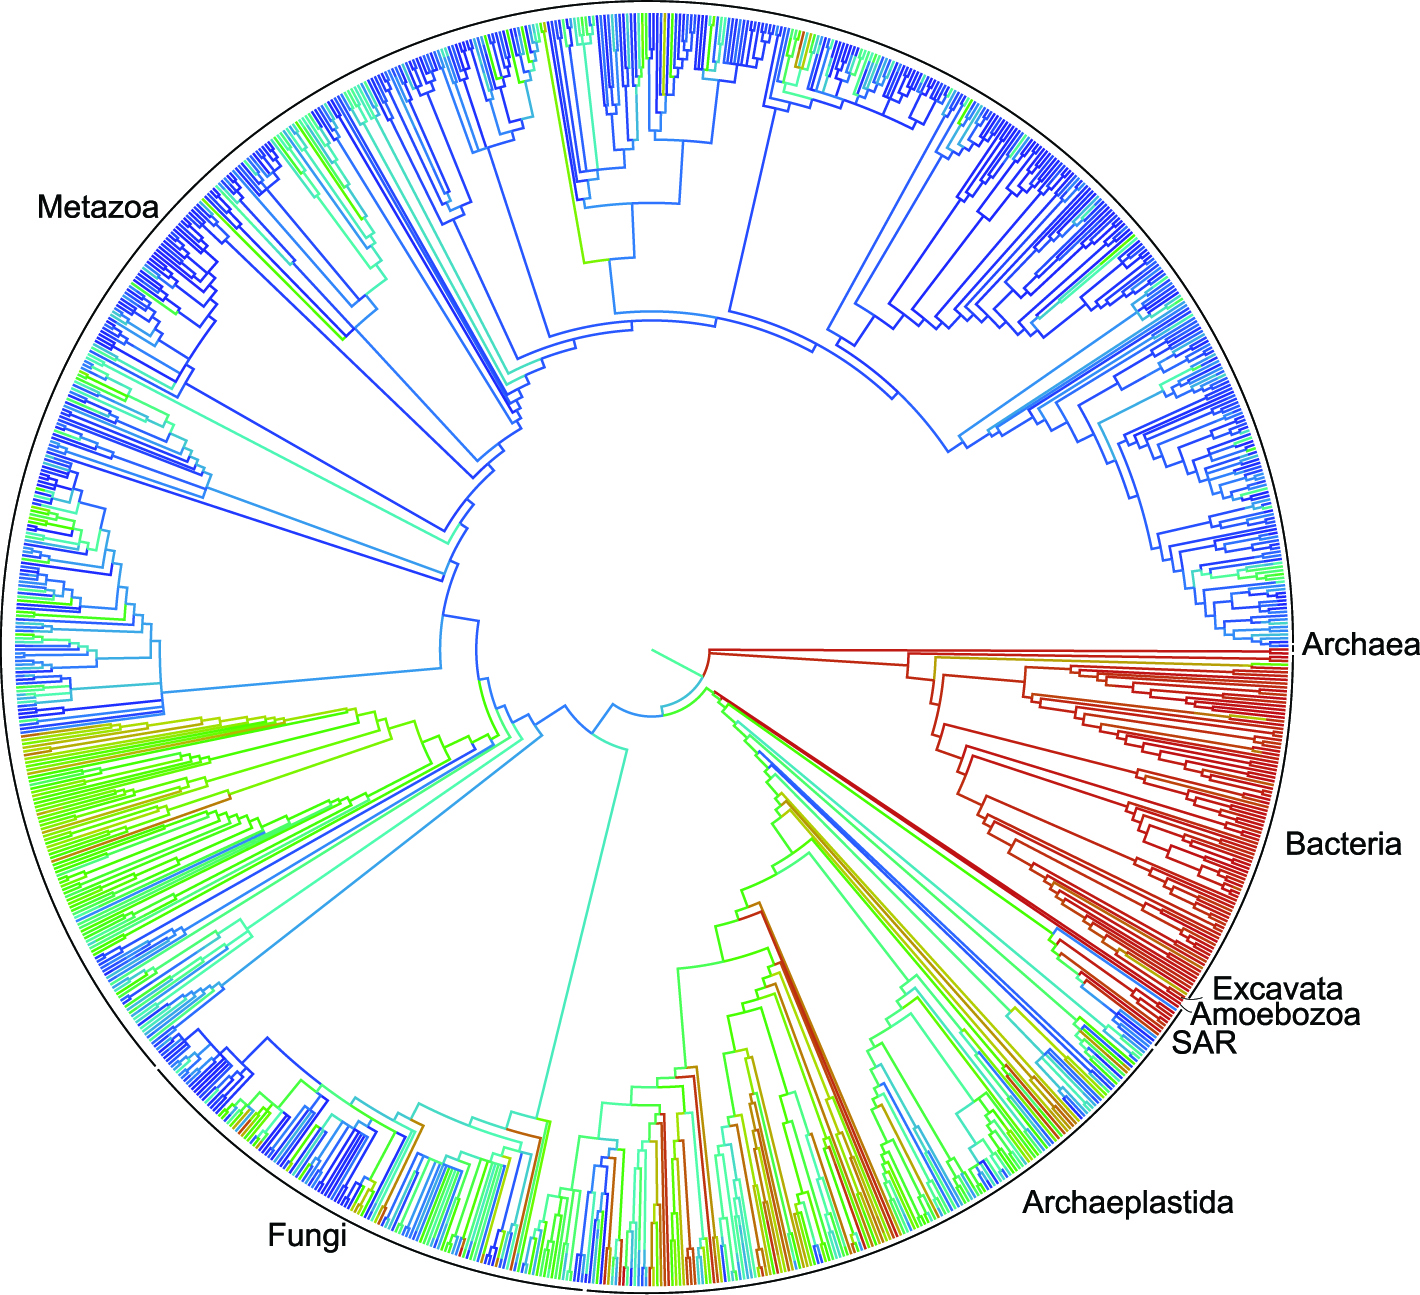
\includegraphics[width=\textwidth]{treeoflife}
	\fonte{\citetexto{Hinchliff2015}.}
\end{minipage}
\end{figure}


%Keane2006a
%The approach that is most commonly taken is to esti-mate the model parameters on some initial tree (Yang, 1994) obtained from a
%distance method and successively optimise the parameters every n iterations
%of the tree search (Guindon and Gascuel, 2003).

%distance based and character based


%\cite{yang2014molecular}
%In theory, methods based on optimality criteria
%have to solve two problems: (i) calculation of the criterion (tree score) for a given tree and
%(ii) search in the space of all trees to identify the tree with the best score. The first problem
%can be expensive if the tree is large, but the second is much worse when the number of
%sequences is greater than 20 or 50 because of the huge number of possible trees. As a
%result, heuristic algorithms are used for tree searches.

%Keane2006a
%In a Markov system, each subsequent
%state of the system is determined by examining only the current state of the
%system
%
%The approach that is most commonly taken is to esti-mate the model parameters on some initial tree (Yang, 1994) obtained from a
%distance method and successively optimise the parameters every n iterations
%of the tree search (Guindon and Gascuel, 2003).
%
%Long branch attraction (LBA) refers to the tendency of species at the ends of
%long branches in a phylogenetic tree to appear artificially close to each other.
%
%HGT is any process in which an organism transfers genetic material to an- other organism that is not its offspring. HGT
%This can
%often produce unexpected phylogenies as other species similar to the recipi-ent (but not involved in the transfer) may be placed in an entirely different
%part of the tree making either the recipient or donor seem out of place.
%
%Heterotachy occurs when the evolutionary rate of a given position in an align-ment changes through time (Lopez et al., 2002). Heterotachy is expected to
%occur frequently in real datasets as different sites will be under contrasting se-lection and adaptive pressures at different points in time.


\subsubsection{Matrizes de Distâncias}

%Keane2006a
%Distance methods
%are often used to gain an initial estimate of the phylogeny that is improved
%upon by more accurate methods (Guindon and Gascuel, 2003; Vinh and von
%Haeseler, 2004).
%\cite{yang2014molecular}
% Distance methods are often computationally faster than
% character-based methods, and can be easily applied to analyse different kinds of data as
% long as pairwise distances can be calculated.

O método de inferência filogenética por matrizes de distâncias, embora não seja mais o estado da arte, continua exercendo importante papel como fundação aos métodos mais complexos existentes atualmente, ao prover uma árvore inicial, que é posteriormente melhorada por métodos mais precisos \cite{Guindon2003,Vinh2004}.
Em função de sua eficiência computacional, sendo geralmente mais rápida do que outros métodos baseados em caracteres, a inferência baseada em matrizes de distâncias pode ser facilmente aplicada em análises de diferentes tipos de dados, contanto, que as distâncias entre pares de amostras possam ser calculadas \cite{yang2014molecular}.
%Devido a inferência baseada em matrizes de distâncias ser computacionalmente eficiente, sendo geralmente mais rápidas do que outros métodos baseados em caracteres e podendo ser facilmente aplicadas em análises de diferentes tipos de dados, contanto, que distâncias entre pares de amostras possam ser calculadas \cite{yang2014molecular}.
No que diz respeito à sua abordagem, este é um método baseado em distâncias e também qualitativo, pois seu resultado é sempre uma única árvore, sendo esta, a melhor, seguindo seus critérios.



%Keane2006a
%In a distance matrix, identical sequences have a distance of zero
%between them and sequences that do not share any common character states
%are given an arbitrarily large distance (Nei and Kumar, 2000).

%Like parsimony, the main advantage of distance
%methods is their speed. However if the distances are not computed with
%the correct substitution model, the distance matrix values can be incorrect
%and subsequently affect the tree topology (DeBry, 1992). 



\subsubsection{Máxima Parcimônia}


Assim como as matrizes de distância, o método de inferência baseado em máxima parcimônia também é capaz de informar uma única melhor árvore com performance otimizada.
Este método é baseado no princípio da \textquoteleft navalha de Occam\textquoteright, que afirma que hipóteses devem ser mantidas tão simples quanto possível, ou seja, assumir a menor quantidade de premissas.
Segundo \citetexto{Keane2006a}, \citetexto{Edwards1963} foram os pioneiros neste método ao propor que a melhor árvore filogenética é aquela que envolve a menor quantidade possível de evolução, implicando que métodos baseados em parcimônia encontrem a árvore com o menor número de substituições e/ou diferenças entre características de um conjunto sob análise.
No que diz respeito à sua abordagem, este método pode ser usado tanto através de distâncias como caracteres e é também qualitativo.
Contudo, apesar de também ser computacionalmente rápido quando comparado a outros métodos, foi demonstrado que pode ser estatisticamente inconsistente sob certas combinações de árvores, o que pode vir a comprometer seus resultados \cite{Felsenstein1978}.



%\cite{Keane2006a}
%The main theory behind parsimony is based on William of Occam’s prin-ciple that the hypothesis should be kept as simple as possible. 
%Parsimony
%methods were first developed by Edwards and Cavalli-Sforza (1963) when
%they proposed that the true phylogenetic tree is the one that involves ‘the
%minimum net amount of evolution’. This means that parsimony methods
%attempt to find the tree that requires the least number of substitutions (or
%differences) between the sequences being examined from the set of all possible
%phylogenetic trees.
%The main advantage of parsimony is that its execution time is typically very small compared to the other methods.


%\cite{yang2014molecular} Felsenstein (1978b) demonstrated that the parsimony method can be statistically incon-sistent under certain combinations of branch lengths


\subsubsection{Máxima Verossimilhança}
\label{sub:bio-max-likelyhood}

Diferentemente dos anteriores, o método baseado em máxima verossimilhança, do inglês \textit{maximum likelihood} (ML), adota uma abordagem estatística baseada exclusivamente em caracteres.
Introduzido por \citetexto{Felsenstein1981}, este método consiste em uma abordagem estatística para buscar o melhor casamento possível (\textit{best--fit}) entre os dados de alinhamentos de sequências e um sistema de substituição filogenética, maximizando, portanto, a semelhança entre as amostras e um sistema de referência.
Embora seja reconhecido por sua precisão, com \citetexto{Hordijk2005} citando múltiplos exemplos de estudos afirmando que a inferência baseada em ML é capaz de encontrar a melhor árvore filogenética com maior frequência que outros métodos, o cálculo de ML é, no mínimo, NP-difícil, conforme demonstrado por \citetexto{chor2005}.
Tal complexidade computacional dificulta seu emprego em análises com grandes números de amostras em alinhamentos de sequências, no entanto, conforme veremos no \autoref{ch:relacionados}, múltiplos aprimoramentos e heurísticas seguem sendo desenvolvidos para melhorar a performance das inferências baseadas em ML.

%1981, Felsenstein
%Felsenstein (1981[64]) introduced the ML framework to phylogenetic inference
%detalhamento do cálculo de ML em \cite{DarribaPHD}
% It plays a central role in statistics and iswidely used in molecu-lar phylogenetics. \cite{yang2014molecular}


%\cite{Hordijk2005}
%A number of computer studies (Kuhner and Felsenstein, 1994;
%Huelsenbeck, 1995; Rosenberg and Kumar, 2001; Ranwez and
%Gascuel, 2002; Guindon and Gascuel, 2003) have shown that
%ML programs can recover the correct tree from simulated datasets
%more frequently than other methods can, which supported numerous
%observations from real data and explains their popularity.


%\cite{Hordijk2005}
%Tree inference in the ML setting is
%computationally hard (Chor and Tuller, 2005), and all practical
%approaches rely on heuristics.


\subsubsection{Inferência Bayesiana}


Assim como os métodos baseados em máxima verossimilhança, os que se apoiam em inferência bayesiana são classificados por sua abordagem com base em caracteres e em métodos estatísticos.
Outra semelhança está no fato de que as análises feitas utilizando-se de inferência bayesiana também buscam o melhor casamento possível entre os dados e um sistema de substituição filogenética.
Embora também seja baseada em métodos estatísticos, a inferência bayesiana tem como diferença fundamental o fato de que as probabilidades representam o grau de convicção em uma hipótese, ao invés da frequência com que ela ocorre \cite{Keane2006a}.
Nesta abordagem é possível alimentar o conhecimento \textit{a priori}, para que ele contemple informações sobre o processo evolutivo, como o processo de ramificações de Yule \cite{Edwards1970}, e o de nascimento e morte por \citetexto{Rannala1996}, de forma que estes processos possam exercer influência sobre o resultado da distribuição estatística \cite{yang2014molecular}.
O motor por baixo de grande parte das ferramentas de inferência bayesiana é o 
algoritmo Metropolis-Hastings, também conhecido como Markov chain Monte Carlo (MCMC) que, através de uma abordagem baseada em Simulações de Monte Carlo, visita amostras do espaço de busca e, dadas amostragens suficientes, pode ser usada para estimar valores como a média e desvio padrão da distribuição \textit{a posteriori} \cite{Nascimento2017}.


%Keane2006a
%one of the main differences in bayesian
%estimation is that it is possible to include prior information about the phy-logeny (or model) through a prior distribution of trees (or model priors).


%\cite{yang2014molecular}
%In Bayesian statistics, probability is defined to represent one’s degree of belief rather than
%a frequency.
%
%
%The prior can also be specified by modelling the physical/biological
%process. For example, the Yule branching process (Edwards 1970) and the birth–death
%process (Rannala and Yang 1996) can be used to specify the probability distribution of
%phylogenies.
%
%
%\cite{Nascimento2017}
%The workhorse underlying all modern Bayesian phylogenetic
%programs is the Markov chain Monte Carlo (MCMC) or Metropolis–
%Hastings algorithm21,22.
%. However, the MCMC algorithm is both art
%and science, and a basic understanding of its workings is essential
%for the correct use of those programs.
%
%
%involves multidimensional integrals
%and may be too expensive to compute. Thus, MCMC is particularly
%suitable for Bayesian computation. Instead of calculating the
%posterior distribution f(θ |D), the algorithm generates a sample from
%the posterior, which can be used to estimate the mean, the standard
%deviation of the posterior or even the whole posterior distribution.
%
%
%the algorithm visits parameter values with a high poste-rior more often than those with a low posterior. Indeed, it visits the
%parameter values exactly in proportion to their posterior. One runs
%the algorithm over many iterations, and then uses the visited val-ues of d and κ to construct a histogram to estimate the posterior
%distribution or to calculate the mean and standard deviation of the
%posterior
%
%
%The convergence rate is the rate at which a
%chain starting from any initial position (which may be in the tails of
%the posterior) moves to the high-posterior region of the parameter
%space81
%.
%space81
%. Parameter values sampled before reaching this stationary
%phase are usually discarded as the burn-in.
%
%
%Mixing efficiency refers to how efficiently the chain traverses the
%posterior after it has reached the stationary distribution. If the chain
%is more efficient, the estimate based on the MCMC sample will have
%a smaller variance, and the results will show less variation among
%independent runs
%
%
%Both convergence and mixing problems can be diagnosed by
%using a trace plot,
%
%
%With fast convergence,
%different chains that
%started from very different
%positions become indistinguishable very quickly. Efficient mixing
%is indicated by different runs generating nearly identical means,
%standard deviations, and histograms. If the runs are healthy,
%samples from different runs can be combined to produce posterior
%summaries.



\subsection{Sistemas de Substituição de Sequências Moleculares}
\label{sec:modelos-de-substituicao}


\begin{table}[tb]
	\centering%
	\begin{minipage}{\defaultFigureWidth\textwidth}
		\caption{Lista dos mais utilizados sistemas de substituição de sequências moleculares.}
		\label{tab:models}
		\vspace{1ex}
		\begin{tabu} to \textwidth{YX[2.5]@{}}
			\toprule
			Sistema & \multicolumn{1}{c}{Bibliografia} \\ 
			\midrule
			JC69      & \citetexto{JukesCantor1969} \\
			K80       & \citetexto{Kimura1980} \\
			F81       & \citetexto{Felsenstein1981} \\
			F84       & \citetexto{Yang1994}, originalmente implementado por\newline Felsenstein no \textit{software} DNAML a partir de 1984\\[-2ex]
			HKY85     & \citetexto{Hasegawa1984} \\
			TN93      & \citetexto{Tamura1993} \\
			GTR (REV) & \citetexto{Tavare1986} \\
			UNREST    & \citetexto{Yang1994m} \\
			\bottomrule
		\end{tabu}
		\fonte{Elaborado pelo autor com base em \citetexto{yang2014molecular}.}
	\end{minipage}
\end{table}

%Keane2006a
%In a Markov system, each subsequent
%state of the system is determined by examining only the current state of the
%system
%
%

% All phylogenetic methods make assumptions, whether explicit or implicit, about the process of DNA substitution (Felsenstein, 1988).

Uma característica comum aos métodos mais modernos de inferência filogenética é o uso explícito de modelos ou sistemas de substituição.
Seu uso surge da necessidade de estimar a probabilidade das alterações em um conjunto de sequências genéticas, com cadeias de Markov de tempo contínuo figurando como uma das abordagens mais utilizadas \cite{yang2014molecular}.
Embora \citetexto{Felsenstein1988} afirme que todos os métodos filogenéticos dependam de hipóteses, sejam implícitas ou explícitas, sobre os processos de substituição de nucleotídeos e proteínas, somente os métodos baseados em máxima verossimilhança (ML) e inferência bayesiana dependem explicitamente destes sistemas, que nada mais são do que formalizações matemáticas das hipóteses do método utilizado.


\begin{equation}
\label{eq:markovdna}
Q = \begin{pmatrix}
-\mu_A & \mu_{AG} & \mu_{AC} & \mu_{AT} \\
\mu_{GA} & -\mu_G   & \mu_{GC} & \mu_{GT} \\
\mu_{CA} & \mu_{CG} & -\mu_C   & \mu_{CT} \\
\mu_{TA} & \mu_{TG} & \mu_{TC} & -\mu_T 
\end{pmatrix}
\end{equation}


Um dos componentes mais importantes em um cadeia de Markov é a matriz de transição, exemplificada na \autoref{eq:markovdna} por uma matriz de transição para DNA (A,G,C,T), que, no caso dos sistemas de substituição de sequências moleculares costuma indicar a frequência com que as transições de estados ocorrem, assim como a distribuição de ocorrência de cada estado, ilustradas na \autoref{fig:models}.
Neste contexto, os estados são as diferentes proteínas ou nucleotídeos representados pelas possíveis bases, no caso de DNA, como demonstra a \autoref{tab:dna-codes}.
Assim, um dos fatores determinantes de diferenciação entre os sistemas de substituição disponíveis são: 
\begin{inparaenum}[\itshape a\upshape)] 
	\item a configuração da sua matriz de transição;
	\item a distribuição de ocorrências de estados;
	\item o número de parâmetros livres utilizados no sistema.
\end{inparaenum}

%Keane2006a
%
%Therefore, knowing the process of evolution and be-ing able to construct realistic models of evolution is the foundation for being
%able to infer accurate phylogenetic relationships among species (Yang, 1994;
%Yang et al., 1998; Sullivan and Swofford, 1997; Posada and Buckley, 2004).
%
%Therefore, the model of substitution used in the likelihood calculation plays
%a very important role in inferring phylogenies.

Dada a importância dos métodos de inferência filogenética baseados em ML e Bayes, \citetexto{Keane2006a} afirma que conhecer os processos de substituição e conseguir construir sistemas realísticos é um dos fatores determinantes para habilitar uma correta inferência dos relacionamentos entre espécies.
Dentre uma vasta gama de sistemas disponíveis, apresenta-se na \autoref{tab:models} uma lista dos mais populares conforme \citetexto{yang2014molecular}.
Contudo, apesar dos grandes avanços na modelagem do processo evolutivo, existem uma série de falhas conhecidas pela comunidade filogenética e que devem ser cuidadosamente verificadas antes de tomada uma decisão a respeito do sistema a ser usado para qualquer tipo de análise.
\citetexto{Keane2006a} fornece uma lista das mais reconhecidas fraquezas presentes nos sistemas:


\begin{itemize}
	
	\item \textbf{Atração por Longas Ramificações (LBA\footnote{do inglês, Long Branch Attraction.}):}
	%Long branch attraction (LBA) refers to the tendency of species at the ends of
	%long branches in a phylogenetic tree to appear artificially close to each other.
	refere-se à tendência de organismos posicionados ao final de longas ramificações de uma árvore filogenética de parecer artificialmente perto um do outro;
	
	\item \textbf{Transferência Horizontal de Genes (HGT\footnote{do inglês, Horizontal Gene Transfer.}):}
	%HGT is any process in which an organism transfers genetic material to an- other organism that is not its offspring. HGT
	%This can
	%often produce unexpected phylogenies as other species similar to the recipi-ent (but not involved in the transfer) may be placed in an entirely different
	%part of the tree making either the recipient or donor seem out of place.
	é um processo em que um organismo transfere material genético para outro organismo que não pertence à sua descendência, o que pode produzir filogenias inesperadas, uma vez que espécies similares ao receptor (mas não envolvidas na transferência) podem ser transferidas para uma parte completamente diferente da árvore, fazendo com que tanto o doador quanto o receptor possam parecer deslocados;
	
	\item \textbf{Heterotaquia\footnote{do inglês, Heterotachy.}:} 
	%Heterotachy occurs when the evolutionary rate of a given position in an align-ment changes through time (Lopez et al., 2002). Heterotachy is expected to
	%occur frequently in real datasets as different sites will be under contrasting se-lection and adaptive pressures at different points in time.
	denomina a ocorrência de variações ao longo do tempo na taxa evolutiva considerada normal para uma posição de uma sequência molecular, confundindo sistemas que assumem uma taxa evolutiva constante, sendo esta uma premissa que não necessariamente se mantém por todo o histórico de um organismo devido às diferentes pressões evolutivas durante sua história.

\end{itemize}


Portanto, é fundamental que a escolha de um sistema de substituição para análises filogenéticas seja embasada em dados a respeito das múltiplas sequências moleculares em estudo e que respeite as características da análise, seja ela, a respeito de uma determinada região de interesse ou de toda a sequência genética do organismo; se contempla múltiplas espécies; ou ainda, se abrange um longo período de tempo.
\citetexto{Zwickl2006} justifica a necessidade de extremo cuidado na escolha do sistema afirmando que:


% \cite{Zwickl2006b}
%Choosing a model that is too
%simple (underfitting) causes the model to be unable to fully capture the process of
%substitution that generated the data, and can reduce the accuracy of tree inference.
%Choosing a model that is overly complex (overfitting) may reduce the power of tree
%inference because some parameters may fit random noise present in the data rather than
%true phylogenetic signal. With real biological data, any model we choose will inherently
%be a simplification, and so our task is to choose the best available model, rather than
%“true” model.


\begin{quote}
	escolhendo um sistema excessivamente simples, perde-se a capacidade de capturar totalmente as nuances do processo de substituição que gerou os dados, reduzindo a precisão da análise;
	de modo inverso, a escolha de um sistema muito complexo traz consigo o risco de reduzir o poder da inferência no evento em que alguns parâmetros podem contemplar ruído presente nos dados ao invés de verdadeiros sinais filogenéticos;
	no entanto, ao trabalhar com dados biológicos reais, \emph{qualquer sistema escolhido será inerentemente uma simplificação, de forma que a tarefa é encontrar o melhor sistema possível} ao invés do 'verdadeiro' sistema.
\end{quote}


%\cite{DarribaPHD}
%Selecting the best-fit model of evolution requires the scoring of every candi-
%date model. Typically, this requires the optimization and evaluation of each of the competing models such that they can be compared to each other. We cannot ensure that the optimal likelihood score is achieved for each of the models, and also the optimization methods used for optimized each of the parameters might get stuck in local op-tima.


\begin{figure}[tb]
	\centering%
	\begin{minipage}{\defaultFigureWidth\textwidth}
		\caption[Taxas relativas de substituição para três sistemas baseados em cadeias de Markov]{Taxas relativas de substituição para três sistemas baseados em cadeias de Markov: a grossura das linhas representa a probabilidade de transição e o tamanho dos círculos representa a distribuição de ocorrências}
		\label{fig:models}
		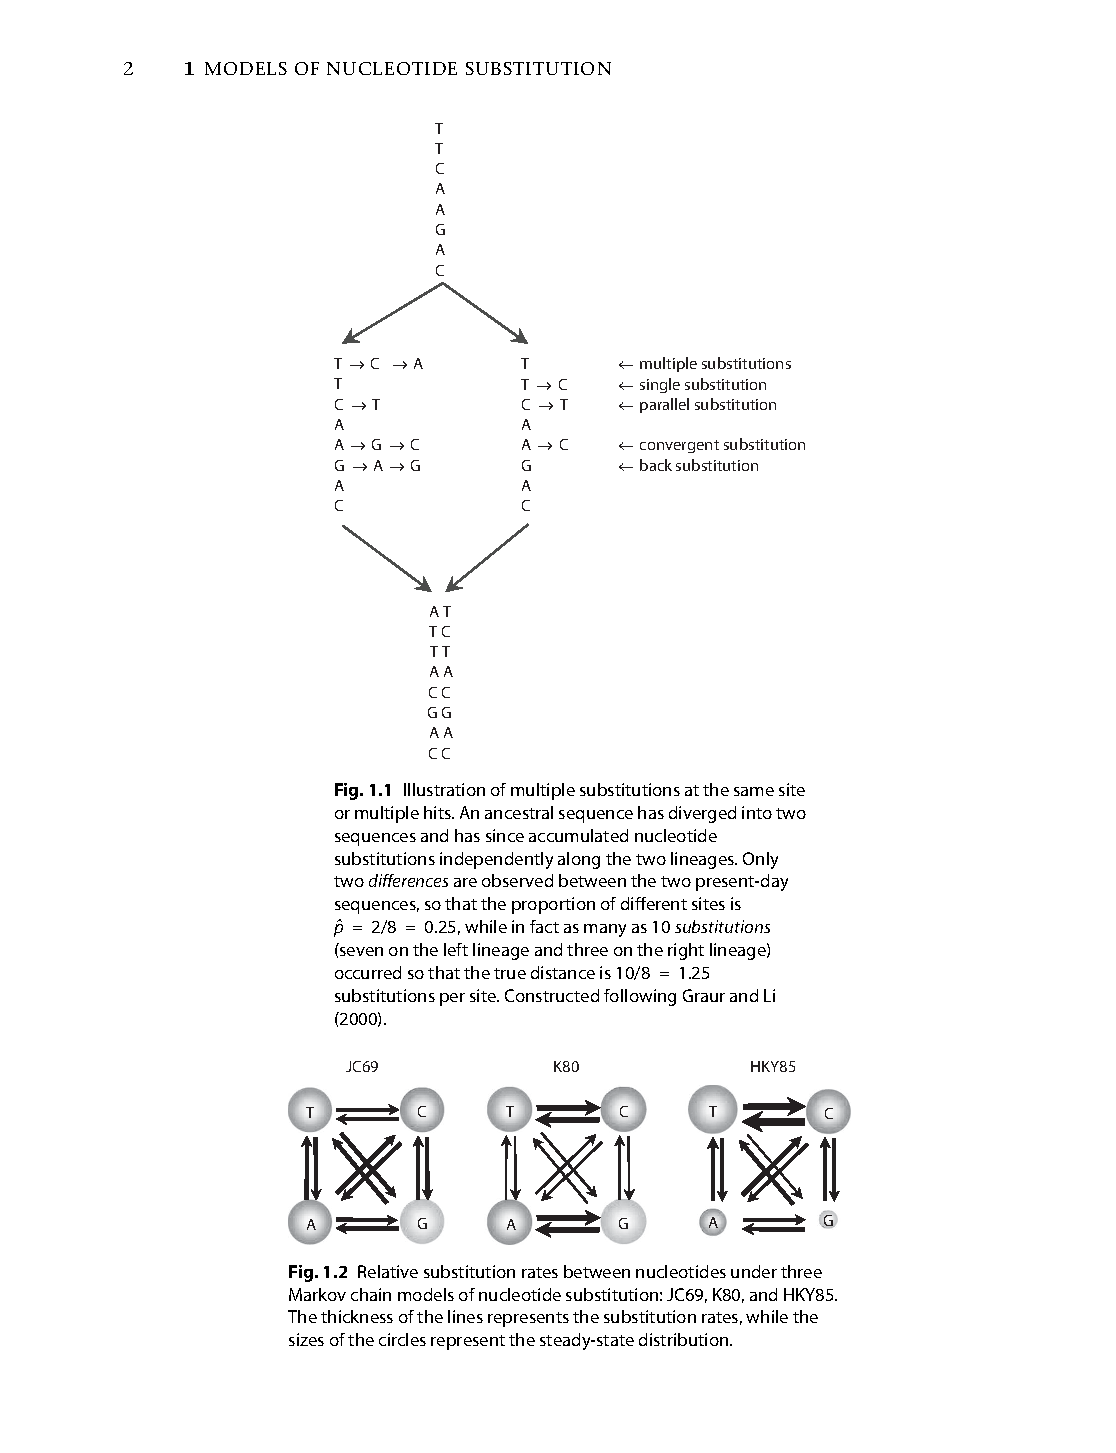
\includegraphics[trim=130 95 120 500,clip,width=\textwidth]{yang2014molecular-fig1-2}
		\fonte{\citetexto{yang2014molecular} referenciando os sistemas \citetexto{JukesCantor1969}, \citetexto{Kimura1980} e \citetexto{Hasegawa1984}, respectivamente.}
	\end{minipage}
\end{figure}




\section{Computação de Alto Desempenho}
\label{sec:computacao}


%TOD0: Na parte de fundamentação teórica, seria legal a gente trazer algo que o problema é computacional muito intenso de ser resolvido, com citações. Isso tb aparece como tua motivação na parte do modelo. [gmail FMfcgxwBTsfLXGPKcBNKhxLncfDftgCR]


Com o objetivo de impulsionar a pesquisa e fornecer respostas para os cada vez mais complexos problemas de variados campos do conhecimento, os supercomputadores e clusters estão na vanguarda dos projetos computacionais.
Inicialmente projetados com hardware e software específico, como era o caso dos Cray, na década de 60, ao longo dos anos os sistemas de computação de alto desempenho foram convergindo em suas tecnologias e definindo tendências nesse sentido.
Recentemente, o design de supercomputadores e sistemas de alto desempenho tem sido dominado, do ponto de vista de hardware, por componentes ``de prateleira'', ou seja, disponíveis para usuários finais, e por um aumento no paralelismo através de processadores com múltiplos cores e GPUs.


Embora este tipo de sistema esteja, classicamente, restrito a centros de pesquisa e universidades com grandes orçamentos, os aprendizados obtidos na construção e operação de supercomputadores têm sido compartilhados com a comunidade em geral através de métodos e algoritmos publicados em revistas científicas.
Tais ensinamentos eventualmente alcançam o público em geral e passam, conforme sua utilidade, a se tornar parte da rotina do desenvolvedor de software.
\textit{Clusters} caseiros e a computação em nuvem, conforme veremos a seguir, contribuem para expandir o acesso a um alto poder computacional que deve ser explorado através de técnicas eficientes e já testadas, como as oriundas da computação de alto desempenho.


Através de técnicas de computação paralela e distribuída torna-se possível tratar problemas que transcendem a capacidade de um único computador, sendo atualmente uma das formas mais amplamente conhecidas de computação de alto desempenho.
O aumento no volume de dados, acompanhado da necessidade de análises cada vez mais profundas fez com que a capacidade de processamento de um único recurso computacional não fosse mais suficiente para atender tais necessidades.
A percepção desta mudança deu origem ao termo \textit{Big Data} e fomentou a visão da empresa orientada a dados, o que, como uma profecia autorrealizadora, agravou ainda mais o problema, dando origem à projetos de software como Hadoop, BigQuery, Spark e Kafka, dentre os mais populares.


O surgimento da computação em nuvem mudou radicalmente a forma como se compra computação em um contexto comercial, influenciando, também, os rumos da pesquisa acadêmica.
Através do modelo de custos baseado no uso, a computação em nuvem possibilita transformar o investimento capital, que incorre da compra de recursos como servidores, equipamentos de rede e pessoal para configuração, em custo operacional, que varia de acordo com o uso acompanhando altos e baixos no consumo de recursos computacionais.
Acessando serviços remotos através da Internet, a computação em nuvem permite acesso ubíquo a recursos computacionais que podem ser rapidamente configurados e requerem gerenciamento mínimo enquanto fornecem ao provedor o benefício das economias de escala.


A elasticidade se posiciona como a principal mudança ocasionada pela computação em nuvem do ponto de vista da computação de alto desempenho, possibilitando o projeto de sistemas que se ajustam conforme a demanda, uma vez que adicionar e remover recursos é uma das funcionalidades oferecidas pelos provedores na forma de uma chamada de função e realizada em questão de minutos.
Esta capacidade de auto serviço via Interfaces de Programaçao de Aplicações (APIs) torna possível a criação e composição de inovadoras soluções computacionais, onde uma aplicação pode alocar e desalocar os recursos necessários para executar determinada tarefa apenas enquanto ela está sendo executada.
Um exemplo deste cenário ocorre no uso de aceleradores gráficos disponibilizados pelos grandes provedores de computação em nuvem na forma de \textit{add--ons} que podem ser atachados a uma máquina virtual (VM) mesmo depois que ela já esteja em uso, desafiando a noção clássica de que um computador contempla um conjunto fixo de recursos definidos em tempo de montagem e \textit{boot} do sistema operacional.
O desafio, portanto, passa a ser qual é a melhor maneira de tirar proveito destas capacidades, uma vez que são possíveis do ponto de vista técnico, alinhando interesses técnicos e econômicos em busca de projetos de software que possam se moldar conforme o uso.


Uma nova abordagem à virtualização utilizada pelos provedores de computação em nuvem é apresentada na forma da orquestração de contêineres, que, ao mesmo tempo que fornecem isolamento entre aplicações, são estruturas mais leves do ponto de vista de sobrecarga computacional por utilizarem o paradigma de virtualização à nível de sistema, ao invés de hardware, como é o caso das máquinas virtuais.
Através do uso de sistemas de arquivos em camadas, contêineres fornecem, além do isolamento, uma camada de portabilidade ao empacotar, na forma de imagens, tanto a aplicação quanto as suas dependências.


Dentre as mais recentes inovações no contexto de computação em nuvem podemos citar o paradigma FaaS, também chamado de \textit{serverless}, que abstrai do desenvolvedor a maior parte das camadas anteriores ao código enquanto fornece um ambiente padronizado com elasticidade automática embutida.
Tal cenário é habilitado pela combinação entre elasticidade de recursos e contêineres, possibilitando o uso de FaaS para execução de códigos pontuais, geralmente limitados em termos da sua duração, e que respondem a eventos.
Desta forma, obtém-se um ambiente verdadeiramente pago pelo uso, onde a cobrança só ocorre quando o código está executando, e não enquanto o recurso está disponível, como acontece nas máquinas virtuais.
Devido as características como o auto grau de elasticidade e a facilidade em obtê-lo, a cobrança pelo uso e a gestão da maior parte da infraestrutura por parte do provedor de computação em nuvem, o paradigma FaaS vem ganhando espaço no âmbito comercial, embora muitos ainda o considerem imaturo.


\subsection{Computação Paralela e Distribuída}
\label{fundamentacao-computacao-distribuida}


%Keane2006a
%The most well-known and commonly referenced parallel architecture classi-fication is Flynn’s taxonomy (Flynn, 1966, 1972; Skillicorn and Talia, 1998).
%Flynn classifies all computers according to two dimensions: instruction and
%data. An instruction stream is defined as a set of instructions to be executed
%on a particular data stream.
%
%As there is a huge variety of machines that can be classed as
%MIMD parallel architectures, it has been suggested that the MIMD classifi-cation is too general and should be further subdivided according to memory
%organisation (Johnson, 1988; Hwang, 1987).


%Experiments in mod-ern scientific research often involve very long computations that can often
%take days, weeks, or even years to complete on a single desktop machine
%(Bohannon, 2005).

%idle computation = 
%This has been exemplified
%by the success of the SETI@home (Korpela et al., 2001) and Folding@Home
%(Shirts and Pande, 2000) projects.


%There are a number of clearly identifiable characteristics that
%a problem should exhibit in order to be suitable for a distributed computing
%implementation (Dubey et al., 1995; Bal et al., 1989; Skillicorn and Talia,
%1998). One of the two most important characteristics is the ability to split
%a problem into independent units that can be processed individually with
%little or no communication required between the sub-blocks. Furthermore, if
%a distributed system is to operate successfully in an environment as diverse
%as the Internet where network communication links vary greatly, the other
%important characteristic is that the volumes of data being transferred across
%the network be kept to a minimum (Bal et al., 1989).


A computação paralela vem sendo amplamente utilizada como forma de obter, em um tempo razoável, respostas para problemas considerados de alta complexidade.
O aumento no volume de dados disponíveis colocou as técnicas de computação paralela e distribuída em maior evidência, uma vez que a demanda por análises cada vez mais detalhadas e descritivas traz benefícios para toda a sociedade \cite{wilkinson1999parallel}.


Projetos de computadores paralelos e distribuídos têm grandes demandas no que diz respeito a qualidade dos equipamentos utilizados. 
Hardware específico com redes confiáveis e de alta velocidade são a norma observada entre os supercomputadores da Top500\footnote{
	Top500 é um projeto que divulga os 500 supercomputadores mais poderosos do mundo.
}.
Entretanto, devido aos altos custos de capital e de operação, tais supercomputadores têm sido gradualmente substituídos por \textit{clusters} de computadores comuns \cite{Baker1999}.


Os benefícios da computação paralela e distribuída certamente compensam as dificuldades em construir e operar um \textit{cluster} ou um supercomputador, no entanto tais dificuldades oneram também a construção das aplicações que farão uso destes recursos. 
Desta forma, os supercomputadores e suas aplicações tendem a ter um alto nível de acoplamento, o que torna tanto o comportamento quanto a performance das aplicações dependente do hardware, da plataforma, das características de rede e de outras particularidades, limitando a escalabilidade \cite{Rajan2011}.

Fornecendo uma base sólida para novos desenvolvimentos, os mais importantes padrões de projeto para computação paralela e distribuída, na visão de \citetexto{wilkinson1999parallel}, são brevemente descritos abaixo.

\begin{itemize}
	\item \textbf{Embaraçosamente paralelos:}
	Caracteriza problemas que podem ser imediatamente decompostos em unidades independentes e balanceadas, requerendo pouco ou nenhum esforço para a divisão das tarefas e a completa independência entre as unidades;
	
	\item \textbf{Divisão e conquista:} 
	Consiste em reduzir um problema em partes sucessivamente menores, de forma que estas possam ser tratadas de forma individual, com maior facilidade. 
	Análoga a recursão em algoritmos sequenciais, a divisão e conquista pode se manifestar na \textit{decomposição de domínio}, ou na \textit{decomposição funcional};
	
	\item \textbf{\textit{Pipelines}:}
	Apropriada para problemas parcialmente sequenciais, esta técnica divide a computação em etapas que devem ser completadas uma após a outra com o paralelismo se manifestando na forma de múltiplas unidades de execução para cada uma das etapas, também chamadas de estágios do pipeline;
	
	\item \textbf{Fases paralelas:}
	Neste modelo, também conhecido por \textit{Bulk Synchronous Parallel} (BSP) os vários processos que correm em paralelo devem, em um determinado momento, chegar a uma barreira onde, obrigatoriamente, devem se comunicar, compartilhando informações de estado, por exemplo, e esperar os demais processos atingirem este mesmo ponto para, só então, prosseguir com sua computação;
\end{itemize}

\subsection{Computação em Nuvem}
\label{sec:cloud}


A computação em nuvem apresenta um novo paradigma computacional trazendo consigo uma forma diferenciada de se pensar em Tecnologia da Informação no que diz respeito a aquisição e manutenção de hardware e datacenters. 
Esta pode ser vista como a combinação entre um conjunto de tecnologias já estabelecidas e conhecidas, mas que juntas possibilitaram a criação de um modelo de operação mais flexível que o tradicional datacenter \cite{Zhang2010}.

Através da Internet, a computação em nuvem provê acesso a infraestrutura e recursos computacionais em escala massiva e com estrutura de custos similar a uma companhia de eletricidade, realizando a ideia teorizada por John McCarthy nos anos de 1960, a computação como um serviço\footnote{
	Do inglês: \textit{utility computing}.
}
\cite{Zhang2010,Suleiman2012}.
Empresas não precisam mais investir grandes capitais em hardware e infraestrutura para implantar seus serviços e nem dos custos operacionais para mantê-los, pois através da computação em nuvem estes custos são diluídos como despesas operacionais e crescem conforme o uso \cite{Martin2011}.

\citetexto{Armbrust:EECS-2009-28}, por meio de estudos em conjunto com os maiores provedores de computação em nuvem, definem as principais características deste paradigma:
\begin{inparaenum}[\itshape a\upshape)]
	\item ilusão de recursos computacionais infinitos, disponíveis sob demanda, deste modo eliminando a necessidade de provisionar capacidade;
	\item dispensa investimento de capital, permitindo começar com pouco e aumentar a alocação de recursos, conforme as necessidades e o ritmo de crescimento; e
	\item pagar pelo uso (por exemplo, servidores por hora e armazenamento por dia), recompensando, desta forma, a conservação de recursos.
\end{inparaenum}


Por ser relativamente jovem e uma combinação entre tecnologias, a obtenção de uma definição amplamente aceita para a computação em nuvem foi um desafio, pois cada autor favorece as características que mais lhe convém.
No entanto a elasticidade e o modelo de custos são consenso, formando a base para que o \textit{National Institute of Standards and Technology} (NIST)\footnote{
	Instituto Nacional de Padrões e Tecnologia, uma agência governamental americana.
} a defina como:

\begin{quote}
	Infraestrutura com capacidades de aprovisionamento de recursos de forma rápida e elástica, em alguns
	casos automática, para aumentar e diminuir o número de recursos. Para o usuário, tais capacidades muitas vezes
	parecem ser ilimitadas, podendo ser realizadas em qualquer quantidade e a qualquer momento.
\end{quote}

Pode-se concluir que a computação em nuvem, por meio da combinação de tecnologias, atinge o objetivo de prover recursos computacionais como um serviço, democratizando e simplificando a computação em larga escala \cite{Awada2017}.
Através da virtualização, é capaz de simular capacidade infinita e reduzir drasticamente os tempos de provisionamento, fornecendo diversos benefícios ao mesmo tempo que impõe novos desafios \cite{Zhang2010}, requerendo, por exemplo, esforços de migração de sistemas, devido a natureza orientada a servidores de aplicações existentes, que torna-se uma significativa barreira de entrada para um grande número de usuários \cite{Jonas2017}.

\subsection{Elasticidade}
\label{sec:elasticidade}

\begin{figure}[tb]
	\centering%
	\begin{minipage}{\defaultFigureWidth\textwidth}
		\caption{Taxonomia da Elasticidade apresentando quais são as Modalidades e Políticas disponíveis além das diferentes estratégias de elasticidade.}
		\label{fig:elasticidade-taxonomia}
		\vspace{1ex}
		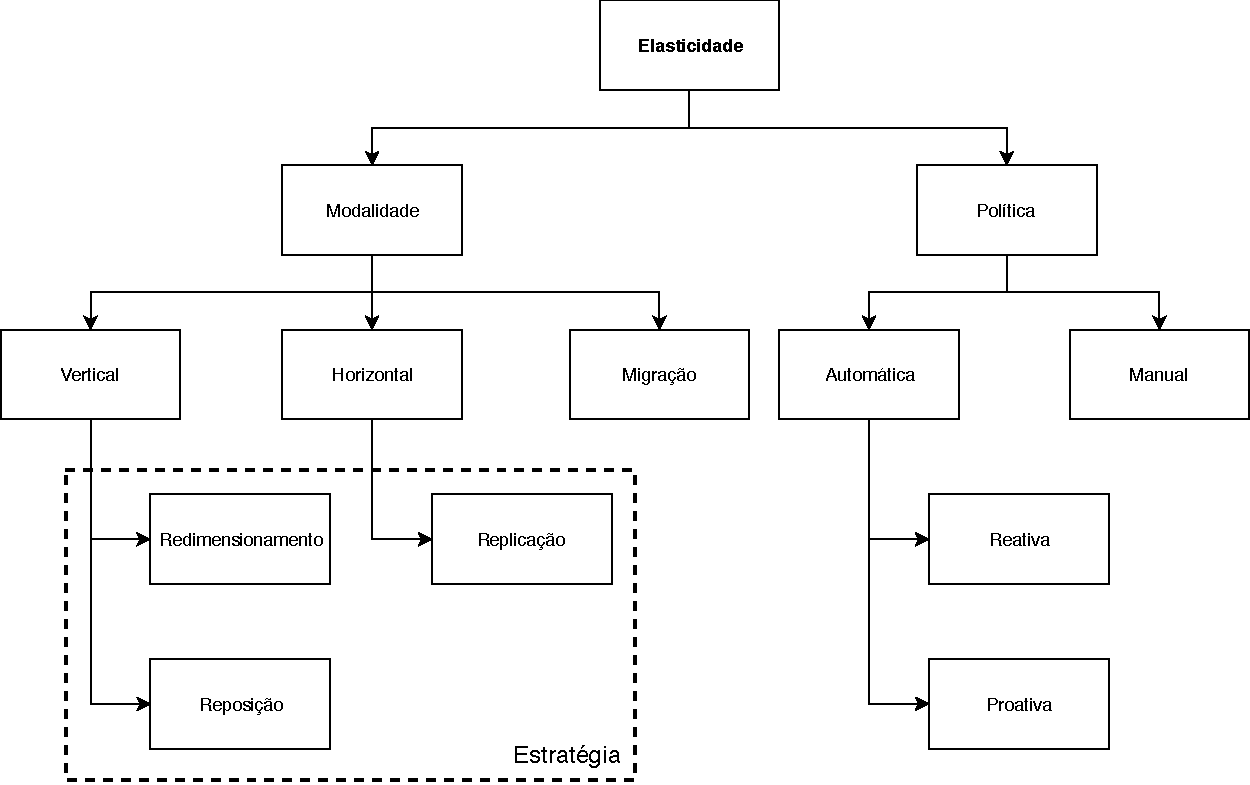
\includegraphics[clip,width=\textwidth]{AUTOELASTIC-taxonomia}
		\fonte{Adaptado de \citetexto{S2016}, \citetexto{Coutinho2015}, \citetexto{Righi2013} e \citetexto{Galante2012}.}
	\end{minipage}
\end{figure}


Dentre as características que definem a computação em nuvem e, talvez, o que efetivamente diferencia este paradigma frente a outras alternativas \cite{Galante2012}, a elasticidade, que diz respeito a capacidade de adicionar e remover recursos computacionais de forma automatizada e com um tempo de provisionamento na casa dos minutos, ao invés de semanas, é a propriedade que permite aos usuários casar a demanda com a alocação de recursos \cite{Armbrust:EECS-2009-28,Raveendran2011,Imai2012,Suleiman2012}.

Segundo \citetexto{Raveendran2011}, projetos de aplicações paralelas e distribuídas tradicionalmente contemplavam um número fixo de recursos, efetivamente definindo um prazo de validade para o investimento, pois esta classe de aplicações costuma ser muito sensível à características do ambiente. 
Tipicamente, recursos computacionais como processamento, rede e armazenamento são finitos e estáticos, sendo inicialmente adquiridos através de uma estimativa da capacidade de pico na esperança de que a carga média fique abaixo desta estimativa. No entanto, enquanto os recursos são estáticos, a demanda é dinâmica \cite{Marshall2010}.

Enquanto a alocação estática tenta provisionar recursos sempre para o pior caso, correndo o risco de errar para mais ou para menos, a alocação elástica depende do comportamento da aplicação, definido através de métricas e níveis de serviço contratados \cite{Righi2013}. 
Os benefícios da alocação elástica se manifestam para todos os envolvidos, onde o usuário consegue manter o desempenho da sua aplicação a um preço justo e o administrador da nuvem otimiza o uso de seus recursos, repassando para outros usuários a capacidade ociosa \cite{Raveendran2011,Righi2013,HennessyPatterson2013}.


Diferentes provedores e middlewares gerenciam elasticidade da forma que melhor lhes convém, o que torna necessária uma classificação destas estratégias para compreender suas diferenças e, com isso, os pontos fortes e fracos de cada estratégia.
Tomando por base as classificações realizadas por \citetexto{Coutinho2015}, \citetexto{Righi2013} e \citetexto{Galante2012}, ilustradas na \autoref{fig:elasticidade-taxonomia}, pode-se categorizar as estratégias de elasticidade segundo as seguintes dimensões:


\begin{itemize}
	\item \textbf{Modalidade:}
	\begin{inparaenum}[\itshape a\upshape)]
		\item vertical: onde substitui-se um recurso por outro com atributos redimensionados, como CPU ou memória, por exemplo; ou
		\item horizontal: onde é alterado o número de recursos, incluindo novas cópias idênticas para apoiar o atual, por exemplo; ou 
		\item migração: onde a VM é realocada para outro servidor com diferentes características, sendo útil para cenários de redução na carga de trabalho, consolidando recursos computacionais.
	\end{inparaenum}
	
	
	\item \textbf{Política:}
	\begin{inparaenum}[\itshape a\upshape)]
		\item manual: onde as ações de elasticidade dependem de impulsos externos à plataforma; ou
		\item automática: onde a própria plataforma decide e executa as ações de elasticidade que podem ser, por sua vez, 
		\begin{inparaenum}[(i)]
			\item reativas: através de um mecanismo de regra-condição-ação; ou
			\item proativas: que, através de análises preditivas, executa ações de elasticidade visando antecipar a carga.
		\end{inparaenum}
	\end{inparaenum}
	
	
	\item \textbf{Estratégia:}
	\begin{inparaenum}[\itshape a\upshape)]
		\item replicação: onde cópias de uma mesma máquina virtual são utilizadas para contribuir com o processamento; 
		\item reposição: onde uma máquina em execução é levada para outro servidor substituto, visando, por exemplo, aumento ou redução de recursos; ou
		\item redimensionamento: onde atributos específicos da máquina virtual são modificados para influenciar no desempenho da computação.
	\end{inparaenum}
\end{itemize}


A precificação dinâmica, um subproduto do uso elástico de recursos computacionais, possibilita a criação de mercados que negociam a capacidade ociosa dos provedores de nuvem (\textit{spot market}) a um preço mais vantajoso, sendo desejável para uma ampla categoria de aplicações científicas e comerciais.
Contudo, esta possibilidade deixa de ser utilizada por tornar ainda mais complexo o cálculo de retorno no investimento em um ambiente de nuvem e porque aplicações não estão preparadas para lidar com a preempção de recursos (que ocorre quando há exaustão da capacidade ociosa) \cite{Jonas2017}.
Neste momento, o corpo de conhecimento da computação paralela e distribuída se torna um aliado, uma vez que um dos requisitos para a elasticidade é uma boa escalabilidade, ou seja, a capacidade de uma aplicação manter sua eficiência e aumentar o consumo de recursos proporcionalmente ao tamanho do processamento \cite{Galante2012,HennessyPatterson2013}.
Por fim fornece, também, estratégias para recuperação (\textit{self--healing}) e alta disponibilidade.


Apesar dos benefícios promovidos pela elasticidade, realizar seu potencial é uma tarefa não trivial devido aos desafios oriundos do desenvolvimento de aplicações aptas a usufruir destas capacidades \cite{Raveendran2011,Loff2014}.
Embora se observe uma mudança nos padrões de aplicações distribuídas em direção a um maior uso de elasticidade \cite{Shankar2018}, aproveitar de maneira eficiente as vantagens dessa característica permanece um desafio mesmo para usuários sofisticados \cite{Jonas2017}.


\subsection{Orquestração de Contêineres}


\begin{figure}[tb]
	\centering%
	\begin{minipage}{\defaultFigureWidth\textwidth}
		\caption[Diagrama ilustrando as principais diferenças no que tange às estratégias de virtualização baseadas em Contêineres e Máquinas Virtuais]{Diagrama ilustrando as principais diferenças no que tange às estratégias de virtualização baseadas em Contêineres (esquerda) e Máquinas Virtuais (direita)}
		\label{fig:docker}
		\vspace{1ex}
		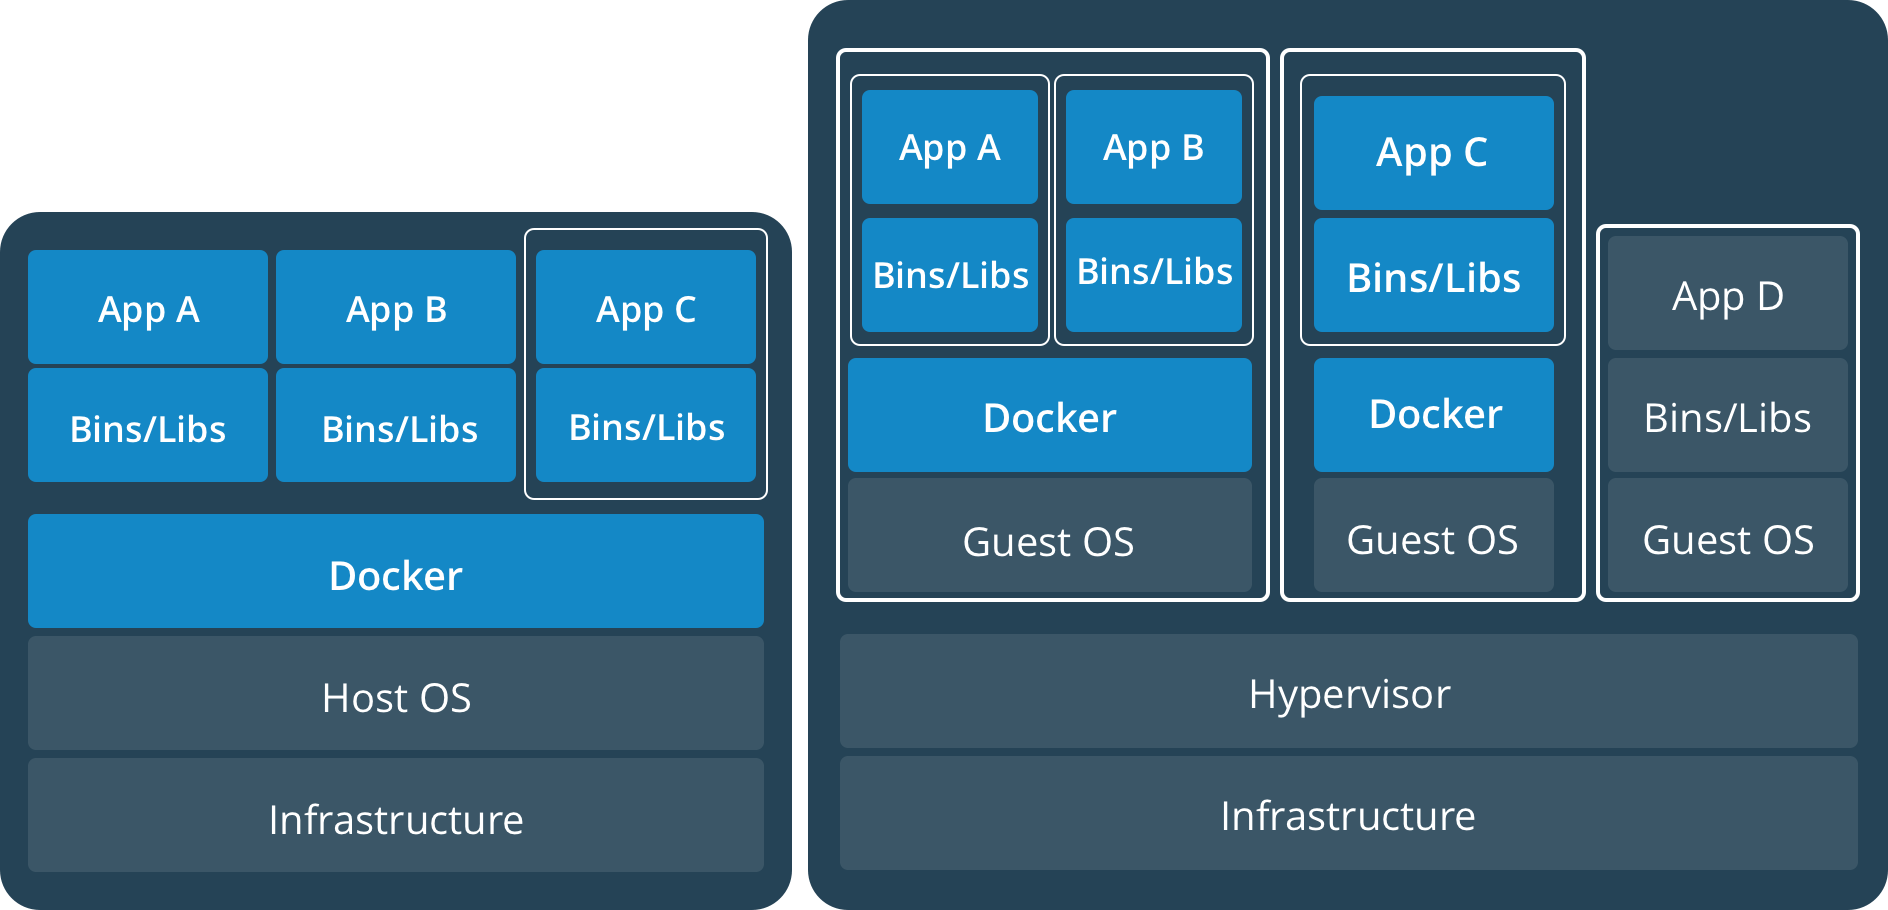
\includegraphics[clip,width=\textwidth]{docker-concept}
		\fonte{Reproduzido de \url{https://www.docker.com/what-container\#/virtual_machines}.}
	\end{minipage}
\end{figure}


Contêineres fornecem isolamento entre aplicações através de mecanismos mais leves que a virtualização completa como ocorre nas máquinas virtuais (VMs) \cite{Awada2017}.
Sua grande vantagem está no fato de que um contêiner, através de uma imagem, guarda um ambiente empacotado, auto--contido e pronto para transporte e publicação de uma aplicação \cite{Pahl2015a}, incluindo, se necessário, bibliotecas e/ou binários de \textit{middlewares} dos quais o software é dependente \cite{Awada2017}.
Essa propriedade favorece a portabilidade do código e é, conforme notado por \citetexto{Higgins2015}, especialmente relevante em um contexto de computação em \textit{grids} remotos, onde o ambiente pode carecer das dependências necessárias para suportar um determinado \textit{job}.


Ainda assim, contêineres são um tipo de virtualização, neste caso, chamada de virtualização à nível de sistema \cite{Tosatto2015} em contraste com a virtualização à nível de hardware, representada pelas VMs, e que incorre uma alta sobrecarga de processamento.
Um dos diferenciais da virtualização por contêineres, e que fornece grandes ganhos de performance, é o seu tratamento do sistema de arquivos por camadas, onde existe permissão de escrita apenas a camada do topo e as demais são composições somente para leitura das camadas restantes, agrupadas em formato de pilha \cite{Higgins2015}.



Contudo, \citetexto{Pahl2015a} pondera que apesar de compartilhar a categoria virtualização, estas duas abordagens solucionam problemas distintos devido aos componentes envolvidos em cada arquitetura, conforme mostra a \autoref{fig:docker}.
Embora máquinas virtuais forneçam um ótimo isolamento e abstração do hardware, o custo necessário para atingir este objetivo é significativo, exigindo uma cópia completa do sistema operacional, a interceptação e tradução de chamadas de sistema e drivers específicos para cada virtualizador \cite{Felter2015}.
Em contrapartida, contêineres fazem uso de diretivas de isolamento e gestão de recursos nativos dos sistemas operacionais, reduzindo significativamente o \textit{overhead} enquanto relaxam as garantias de abstração.
Apesar de parecer uma troca vantajosa, em um ambiente de computação em nuvem é comum que ambas as estratégias sejam utilizadas em conjunto devido às necessidades de isolamento de recursos que os provedores devem assegurar entre diferentes clientes \cite{Bernstein2014}.



Uma das principais implementações de virtualização à nível de sistema é o projeto Docker\footnote{
	Disponível na URL \url{https://www.docker.com}, sem publicações.
} que vem definindo os rumos para abordagens concorrentes.
Seu funcionamento é, assim como boa parte dos projetos similares, baseado em duas funcionalidades do \textit{kernel} do Linux, nomeadas: \textit{cgroups} e \textit{namespaces} \cite{Pahl2015a}.
A partir da sua combinação se torna-se possível isolar aplicações, dando a impressão de que cada uma delas têm o sistema operacional dedicado para si, e limitar o consumo de recursos, especificando de antemão os limites aplicáveis a cada software que roda dentro de um contêiner \cite{Tosatto2015}.
Para especificar o empacotamento é usado um arquivo chamado \textit{dockerfile}, que detalha os elementos que compõem a imagem, assim como as instruções para sua construção.



Embora diversos provedores de computação em nuvem forneçam diretivas para ajustar a quantidade de recursos à demanda, chamadas de \textit{auto--scaling} \cite{Mao2011}, seu aproveitamento e potencial de economia são limitados pelo delay com que VMs são adicionadas e removidas ao \textit{pool} de recursos \cite{Shankar2018}.
Contêineres, por sua vez, devido à sua portabilidade e baixa sobrecarga computacional, costumam ser utilizados para melhorar a utilização de recursos e possibilitar uma densidade de processos mais alta, o que levou à popularização de ferramentas de \textit{deployment} baseadas em contêineres, com diversos projetos comerciais e acadêmicos se propondo a gerir ambientes baseados em contêineres.



Projetos como o Omega \cite{Schwarzkopf2013} e Borg \cite{Verma2015} que, eventualmente, levaram ao Kubernetes\footnote{
	Principal orquestrador de contêineres atualmente e que traça suas origens ao projeto de gestão de \textit{datacenters} Borg, nunca publicamente revelado, mas que influenciou diversas iniciativas (como o próprio Mesos), disponível na URL \url{https://kubernetes.io}.
} \cite{Burns2016}, todos oriundos do Google, além do Mesos\footnote{
	Projeto originalmente criado para gestão de \textit{datacenters} mas que tem se articulado para tornar-se um produto centrado em contêineres, disponível na URL \url{http://mesos.apache.org}.
} \cite{Hindman2011}, do Twitter, são propostas para facilitar a gestão de ambientes baseados em contêineres, seja localmente ou em um ambiente de computação em nuvem.
Ao mesmo tempo os principais provedores anunciam, também, suas respectivas implementações, fornecendo plataformas que possibilitam aos usuários criar \textit{clusters} e gerenciar instâncias de contêineres de maneira automatizada visando maximizar o aproveitamento de recursos como memória e CPU ou prover alta disponibilidade. Sendo os mais populares: Elastic Container Service (ECS\footnote{
	Disponível na URL \url{https://aws.amazon.com/ecs}.
}) da AWS, Azure Kubernetes Service (AKS\footnote{
	Disponível na URL \url{https://azure.microsoft.com/en-us/services/kubernetes-service}
}) da Microsoft e o Kubernetes Engine\footnote{
	Disponível na URL \url{https://cloud.google.com/kubernetes-engine}
} na própria Google Cloud Platform (GPC).


%Pahl2015a
%VMs and containers are both virtualisation techniques,
%but solve different problems.
%-
%VM instances as guests use isolated large files
%on their host to store their entire file system and run typi-cally a single, large process on the host.
%-
%a space concern that trans-lates into RAM and disk storage requirements and is slow
%on startup
%-
%holds packaged self-contained, ready-to-deploy parts of applications and, if necessary, middle-ware and business logic (in binaries and libraries) to run
%applications
%-
%traditional VMs and containers shall be compared in
%order to summarise the two technologies,



%Higgins2015
%shared.This provides functionality similar to a VM but with a lighter
%footprint.
%-
%especially in grid systems where a remote resource may lack the libraries or sup-port software required by a job.
%-
%This allows multiple containers to
%share common image layers, potentially reducing the amount of data required to
%transfer between systems.



%Tosatto2015
%virtualization with hypervisors introduces a not neg-ligible overhead on resources utilization [5] and also the boot
%process of VMs affects the overall latency of the system.
%-
%Hardware virtualization (aka Hypervisors)
%System-level virtualization (aka Containers)
%-
%the same host can achieve higher densities with containers
%than with VMs.
%-
%several different implementations of
%system-level virtualization relies mainly of two kernel features,
%namespaces and cgroups:
%-
%Images are static snapshots of the
%containers’ configuration. Images are read only and incremen-tal,
%-
%The Dockerfile is the file that
%contains simple instructions that build Docker images.
%-
%Using containers, distribuited systems can scale up and down
%according to their load more rapidly than with traditional VMs.

\subsection{Serverless e FaaS (Function as a Service)}\label{sec:faas}



Considerado o próximo passo na evolução de tecnologias oriundas da computação em nuvem, o paradigma \textit{Function as a Service} (FaaS), também conhecido como \textit{serverless}, surgiu como iniciativa dos provedores de computação em nuvem, estreando com o AWS Lambda em 2014, ao fornecer uma nova camada de abstração focada em melhorar o comportamento de elasticidade e aumentar a granularidade dos intervalos de cobrança por recursos utilizados.
O principal fator de diferenciação para esta emergente arquitetura de desenvolvimento de aplicações está, segundo \citetexto{Wang2018}, no fato de que ela isola do usuário tudo o que diz respeito a gestão de servidores, originando o nome \textit{serverless}.


Por ser uma abordagem relativamente nova, ainda não há consenso quanto a definição precisa de FaaS embora diversos autores concordem no que diz respeito aos pontos centrais.
Este cenário pode ser ilustrado através de citações provenientes de três fontes diferentes: \citetexto{Wang2018}, \citetexto{Shankar2018} e o Google Cloud Platform (GCP).
\begin{quote}
	componentes pequenos, autônomos e \textit{stateless} dedicados a lidar com tarefas específicas sendo, na maioria dos casos, um pequeno bloco de código escrito em linguagem de \textit{scripting} que têm seus ambientes de execução e servidores gerenciados pelo provedor de computação em nuvem, que aloca recursos de forma dinâmica para garantir sua escalabilidade e disponibilidade.
	\cite{Wang2018}
\end{quote}
\begin{quote}
	provê usuários com acesso instantâneo a uma grande quantidade de recursos computacionais sem o esforço necessário para a gestão de \textit{clusters} possibilitando executar funções orientados a eventos, e \textit{stateless} que incluem restrições sobre o uso de memória e tempo de execução sobre cada invocação.
	\cite{Shankar2018}
\end{quote}
\begin{quote}
	uma solução computacional leve\footnote{lightweight}, assíncrona e baseada em eventos que permite a criação de pequenas funções de finalidade única que respondem a eventos na nuvem sem a necessidade de gerenciar servidores ou ambientes de execução\footnote{runtime environment}.
	\cite{GCP-FaaS}
	
%	a light-weight, event-based, asynchronous compute solution
%	that allows you to create small, single-purpose functions that respond to cloud events without the need to manage a server or a runtime environment.
\end{quote}



\begin{table}[tb]
\centering%
\begin{minipage}{\defaultFigureWidth\textwidth}
	\caption{Comparativo das principais características nas ofertas de FaaS por parte de três grandes provedores de computação em nuvem.}
	\label{tab:FaaS-implementations}
	\small
	\vspace{1ex}
	\renewcommand\arraystretch{1.4}
	\renewcommand {\tabularxcolumn}[1]{>{\arraybackslash}m{#1}}
	\begin{tabularx}{\textwidth}{@{}WYYYY@{}}
		\toprule
		& {AWS \textquoteleft18} & {AWS \textquoteleft17} & {Azure} & {GCP} \\ 
		\midrule
		{Memória (MB)} & $ 64 \times k $ ($k$~=~2,~3,~...,~47) & $ 64 \times k $ ($k$~=~2,~3,~...,~24) & $ 128 \times k $ ($k$~=~2,~3,~...,~12) & $ 128 \times k $ ($k$~=~2,~4,~8,~16) \\
		{Tempo Limite de Execução (minutos)} & 15 & 5 & 10 & 9 \\
		{CPU} & Proporcional a~Memória & Proporcional a~Memória & Fixo & $ 200 $ MHz $ \times j $ ($j$~=~1,~2,~4,~7,~12) \\
		{Sistema Operacional} & Amazon Linux & Amazon Linux & Windows 10 & Debian 8 \\
		{Espaço em Disco (MB)} & 512 & 512 & 500 & > 512 \\
		{Fatores de Cobrança} & {\footnotesize Tempo~de Execução, Memória~Alocada} & {\footnotesize Tempo~de Execução, Memória~Alocada} & {\footnotesize Tempo~de Execução, Memória Consumida} & {\footnotesize Tempo~de Execução, Memória~Alocada, CPU~Alocada} \\ 
		\bottomrule	\end{tabularx}
	\fonte{Atualizado pelo autor, adaptado de \citetexto{Wang2018}.}
\end{minipage}
\end{table}


Comparando-se ao paradigma mais popular de computação em nuvem, o \textit{Infrastructure as a Service} (IaaS) que é baseado no aluguel de máquinas virtuais cobradas por hora, as FaaS tem como uma das suas maiores diferenças os limites de memória, tempo de execução e, principalmente, o modelo de cobrança, destacados na \autoref{tab:FaaS-implementations}. 
Apesar da computação em nuvem permitir que o hardware dedicado local seja substituído por recursos pagos pelo uso e dinamicamente alocados, \citetexto{Eivy2017} destaca que a cobrança não deixa de ser baseada na alocação, ainda que por hora, ao invés do uso efetivo, fazendo com que o consumidor pague mais do que o necessário por recursos alocados, mas não necessariamente utilizados na sua completude.



Desta forma, o modelo de cobrança FaaS apresenta uma evolução  ao cobrar baseado no tempo de execução de uma função \cite{FowlerServerless, Wang2018}, geralmente arredondado para a casa das centenas de milissegundos (\textit{100ms}), o que significa que o usuário só paga pelo tempo em que seu código está efetivamente executando.
Contudo, os operadores de computação em nuvem cobram seu preço pelas funcionalidades disponíveis no modelo FaaS, com valores contendo um ágio de aproximadamente $2x$, segundo \citetexto{Jonas2017}, quando comparados com VMs de capacidade similar, o que ainda configura um preço aceitável para este autor, uma vez que a cobrança ocorre de forma mais granular, a elasticidade e paralelismo massivos e o fato de que não é incomum encontrar \textit{clusters} utilizando apenas 50\% de suas capacidades.



Segundo \citetexto{Wang2018}, uma execução de FaaS geralmente ocorre em um tipo de \textit{sandbox}, seja um contêiner de função ou uma máquina virtual, que impõem limites sobre fatores como memória, tempo de CPU e tempo máximo de execução.
Desta forma, uma instância da função só será criada quando houver uma solicitação de execução e será congelada imediatamente após seu término, uma visão que é compartilhada por \citetexto{FowlerServerless} e que atribuem este comportamento ao fato de que os contêineres computacionais que executam as funções são efêmeros, criados e destruídos pelo provedor puramente em função da demanda.



Um ponto amplamente divulgado pelos provedores de FaaS e endossado pela academia é o fato de que as execuções de funções são fundamentalmente elásticas, com cada invocação sendo potencialmente executada por um processo paralelo e distribuído, independente e isolado dos demais em função da natureza \textit{stateless} das funções \cite{SpoialaServerless,Jonas2017,FowlerServerless,Jonas2017}.
Apesar de existirem, ao contrário do que sugere o nome, servidores rodando o código submetido, estes não são preocupações do ponto de vista do desenvolvedor \cite{SpoialaServerless}, que se abstém de tarefas como instalação, otimização e atualização de sistemas operacionais, \textit{runtimes} e hardware.
Desta forma a gestão do ambiente e da elasticidade é transferida para o provedor de computação em nuvem, escalando tais funções de maneira automática e dependendo apenas da quantidade de recursos disponíveis em sua plataforma e a demanda de uso por seus clientes \cite{BoweiHan}.


\begin{figure}[tb]
	\centering%
	\begin{minipage}{\defaultFigureWidth\textwidth}
		\caption{Diagrama representando a divisão de responsabilidades sobre as diversas camadas que compõem um ambiente computacional contrastando ambientes locais com diferentes modelos de serviço habilitados pela computação em nuvem (IaaS, PaaS, Contêineres,e FaaS).}
		\label{fig:faas}
		\vspace{1ex}
		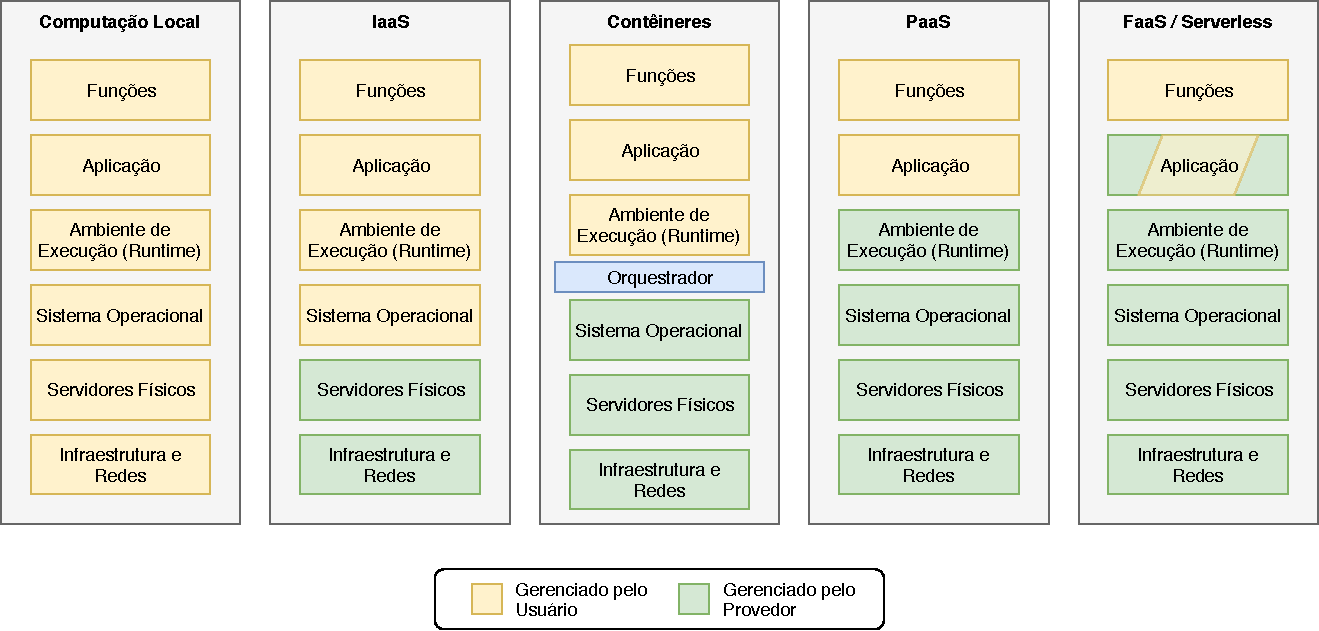
\includegraphics[clip,width=\textwidth]{mestrado-faas}
		\fonte{Adaptado de \citetexto{SpoialaServerless}.} %\url{https://assist-software.net/blog/pros-and-cons-serverless-computing-faas-comparison-aws-lambda-vs-azure-functions-vs-google}.}
	\end{minipage}
\end{figure}



Através deste comportamento inerentemente elástico torna-se possível tirar proveito da elasticidade de uma maneira simplificada, algo que continua desafiador dependendo das características de aplicações e \textit{middlewares}, muitos desenhados originalmente para hardware dedicado \cite{Jonas2017}.
Do ponto de vista da produtividade do desenvolvedor, o emprego de FaaS permite focar apenas nos seus fatores de diferenciação \cite{BoweiHan}, sem preocupar-se com gestão de infraestrutura, \textit{runtimes} e elasticidade, onde \citetexto{Jonas2017} ponderam que não é difícil imaginar um cenário em que o objetivo do usuário não é necessariamente obter a melhor performance possível, mas sim um ganho capaz apenas de superar seus recursos locais sem demandar grande esforço de desenvolvimento.
Ademais, o modelo \textit{serverless} se encaixa bem no contexto do desenvolvimento moderno de aplicações, evoluindo, como mostra a figura \autoref{fig:faas}, para partes reaproveitáveis cada vez menores (conhecidas como \textit{microservices}) que, juntas, compõem a aplicação, contrastando com a construção de aplicações monolítica que se mostram difíceis de gerenciar e escalar \cite{Eivy2017}.


Além dos benefícios para o desenvolvimento, \citetexto{Jonas2017} argumenta que o modelo \textit{serverless} possibilita a criação de sistemas de processamento distribuídos radicalmente mais simples, fundamentalmente elásticos e mais amigáveis do ponto de vista do usuário, características estas, interessantes para a aplicação na pesquisa acadêmica.
\citetexto{Spillner} afirmam, endossando esta visão, que a natureza do provisionamento verdadeiramente sob-demanda, aliada ao modelo de cobrança, torna as plataformas de FaaS atrativas para tarefas de pesquisa, apresentando ainda uma lista (complementada aqui com dados de \citetexto{FowlerServerless}) de implementações do modelo FaaS. Dentre elas:
\begin{itemize}
	\item \textbf{Comerciais:} AWS Lambda, Google Cloud Functions, Azure Functions, Oracle Functions, IBM OpenWhisk;
	\item \textbf{Código Aberto:} Docker--LambCI, Effe, OpenLambda, Fission, OpenFaaS, Kubeless, IronFunctions;
	\item \textbf{\textit{Middlewares}:} Serverless, Claudia.js, AWS Serverless Application Model, Architect.
\end{itemize}


Outro fator relevante das FaaS está relacionado aos ganhos para o provedor de computação em nuvem, com \citetexto{Eivy2017} afirmando que ao oferecer uma plataforma como esta o provedor tem maior controle sob o hardware e software utilizados, possivelmente unificando tudo aquilo que diz respeito às versões, sistemas operacionais, atualizações de segurança e ferramental interno.
Além disso, a natureza \textit{stateless} e de curta duração destas funções facilita a gestão e aumenta a eficiência no aproveitamento de recursos ao garantir a rotatividade necessária para multiplexar clientes e balancear a demanda à oferta de recursos, um fator primordial para a rentabilidade do provedor de computação em nuvem \cite{Shankar2018}.


Apesar dos grandes benefícios no que diz respeito ao modelo de cobrança, amplo paralelismo e a elasticidade nativa, \citetexto{BoweiHan} realiza uma necessária análise dos pontos negativos inerentes ao modelo FaaS, como: 
\begin{inparaenum}[\itshape a\upshape)] 
	\item Redução na Transparência: assim como qualquer abstração, certas partes do sistema saem do controle do desenvolvedor, neste caso, o fato do provedor gerenciar a infraestrutura pode dificultar a investigação e solução de problemas;
	\item Dificuldade de Depuração: como toda a execução se dá no provedor de nuvem e em um ambiente restrito as opções de \textit{debug} são limitadas e ainda muito dependente de \textit{logs} e \textit{traces} de execução;
	\item Elasticidade de Custo: proporcionalmente a elasticidade de recursos, os custos pelo uso de FaaS podem potencialmente sair de controle devido a sua natureza virtualmente infinita de recursos, causando surpresas na hora da cobrança.
\end{inparaenum}


A opacidade do modelo computacional possibilitado pelas FaaS também é destacada por \citetexto{Wang2018} como um impeditivo relevante para adoção por determinadas categorias de usuários, como os que trabalham em ambientes altamente regulados, devido às questões que levanta sobre a qualidade do isolamento entre \textit{tenants}, resistência à ataques e o controle de custos.
Corroborando com este último ponto, se destaca a publicação de \citetexto{Eivy2017}, que dedica parte significativa ao cálculo e explicação do modelo de cobrança \textit{serverless}.
No que diz respeito às dificuldades no desenvolvimento, autores como \citetexto{Jonas2017} expressam uma grande preocupação quanto à maturidade das ferramentas para \textit{debug}, uma situação que só se agrava uma vez que o modelo FaaS incentiva o uso de componentes distribuídos e provê amplo paralelismo, complicando a análise de \textit{logs} e \textit{traces} de auditoria.


Ainda no que diz respeito a maturidade deste modelo computacional, são encontrados argumentos que sugerem um longo caminho de desenvolvimento pela frente, seja por falta de ferramental apropriado, reduzido corpo de pesquisa acadêmico (comprovado pela falta de publicações e a vasta quantidade de referências para blogs e páginas web em \cite{Wang2018}, por exemplo) e, até mesmo, pela falta de uma definição precisa e autoritativa acerca dos conceitos de FaaS e \textit{serverless}, sendo ambos utilizados de maneira intercambiável na indústria.
Atualizações frequentes, por parte dos provedores de computação em nuvem, também comprovam a existência de lacunas no paradigma, com novas funcionalidades e correções figurando frequentemente nos \textit{releases} de versões.



Contudo, apesar das fraquezas expostas, evidências informais apontam que arquiteturas baseadas em FaaS vieram para ficar, devido aos relatos de empresas e indivíduos reportando casos de grandes economias e melhorias de performance através da sua adoção.
No meio acadêmico, os trabalhos de \citetexto{Jonas2017} e \citetexto{Shankar2018} contribuem para este cenário encorajador ao atingir, respectivamente, performances na casa de 40 TFLOP/s com 2800 unidades de execução e  4 TFLOP/s com 180 unidades de execução, enquanto trabalhos como o de \citetexto{Wang2018} fornecem um panorama sobre as características e estratégias utilizadas pelos principais provedores de computação em nuvem nas suas ofertas de FaaS.




%=======================================================================
% Trabalhos Relacionados
%=======================================================================
\chapter{Trabalhos Relacionados}
\label{ch:relacionados}


% as epígrafes nos capítulos são opcionais
\epigrafecap{A fool thinks himself to be wise, \\ but a wise man knows himself to be a fool.}{William Shakespeare}


%rabuske
%Esse capítulo apresenta os trabalhos relacionados com a área dessa pesquisa e suas contribuições para a mesma. Na primeira seção, são apresentados os critérios de seleção dos trabalhos e detalhes sobre a execução da pesquisa. Nas seções subsequentes, são apresentados um resumo de cada trabalho relevante e os resultados obtidos pelos mesmos. Por fim, é feita uma análise comparativa entre os trabalhos e são apresentadas as lacunas na área de pesquisa.

%wunsch
%Baseado nesses conceitos, esse capítulo apresenta um mapeamento sistemático de literatura cujo objetivo foi encontrar trabalhos relacionados que aplicam a Internet das coisas durante o processo de triagem de pacientes no departamento de emergência de hospitais. Sendo assim, foi possível encontrar 16 modelos voltados ao assunto de interesse. Esses artigos foram localizados através de uma técnica de mapeamento sistemático de literatura, que será descrita na primeira seção; a segunda seção traz uma análise comparativa entre os modelos encontrados; e, por fim, na terceira seção desse capítulo, são expostas as lacunas de pesquisa encontradas.


Neste capítulo apresenta-se um levantamento da literatura para a compreensão do estado da arte, apresentando trabalhos relacionados assim como suas contribuições para a área de bioinformática aplicada à filogenética e a computação de alto desempenho.
%
Apresenta-se também a estratégia aplicada no levantamento da literatura, as motivações e as justificativas para a estratégia escolhida. Além de delinear as fontes utilizadas e as questões de pesquisa, destacando as palavras--chaves empregadas e os critérios utilizados para inclusão dos resultados.


Em seguida, elaborou-se uma taxonomia para melhor categorizar e classificar os trabalhos encontrados neste levantamento, para então, realizar uma análise comparativa entre eles e um comparativo estatístico. É de fundamental interesse avaliar os trabalhos em termos do emprego de técnicas de computação de alto desempenho, resultando na \autoref{tab:survey-comparativo}, que apresenta uma visão consolidada dos trabalhos enquanto categorizados pela taxonomia e avaliados em termos das técnicas de computação de alto desempenho.


Por fim, delineou-se o cenário encontrado em termos das suas lacunas no que diz respeito à computação de alto desempenho, principalmente no emprego de computação em nuvem e elasticidade de recursos, estratégias de balanceamento de carga e uso de aceleração por GPUs.


\section{Metodologia de Seleção de Trabalhos}


Com o intuito de mapear o estado da arte, no que diz respeito a ferramentas computacionais relacionadas à filogenética, esta dissertação buscou inicialmente uma estratégia baseada em mapeamento sistemático. Contudo, particularidades da área estudada representaram grandes desafios para a execução de uma análise satisfatória, podendo ser citadas neste sentido as seguintes dificuldades:

\begin{itemize}
	
	\item \textbf{Datas de publicação:}
	Apesar dos grandes avanços em tempos recentes, no que diz respeito a tecnologias de sequenciamento genético e algoritmos, as bases que suportam estes avanços permanecem as mesmas e muito populares entre pesquisadores, de forma que uma restrição do tipo ``ano de publicação'' implica em descartar uma parte relevante do corpo de conhecimento da filogenética e seus alicerces.
	Exemplos que corroboram com esta asserção podem ser encontrados na \autoref{sec:modelos-de-substituicao} (\nameref{sec:modelos-de-substituicao}), tendo boa parte das bases estabelecidas na década de 80 e com trabalhos inciais, e até hoje relevantes, iniciando em 1969;
	
	\item \textbf{Baixa aderência a revistas especializadas:}
	Outra característica da intersecção entre computação e filogenética é a baixa aderência das publicações a revistas especializadas, de maneira que projetos de software são muitas vezes publicados em revistas da biologia, como por exemplo \textit{Systematic Biology}, \textit{Nucleic Acids Research} e \textit{Synthetic Biology}. 
	De modo inverso, revistas especializadas em bioinformática acabam recebendo submissões de trabalhos que apenas utilizam softwares para este fim, sem necessariamente apresentar contribuições no ferramental. Exemplos deste cenário incluem as revistas \textit{Bioinformatics} e \textit{BMC Bioinformatics}.
	Para a computação, a situação é agravada pelo reduzido número de publicações em veículos já estabelecidos como o \textit{IEEE} e \textit{ACM};
	
	\item \textbf{Ausência de divulgação das ferramentas:}
	Por fim, um fator adicional é a maneira como diversos artigos apresentam suas contribuições do ponto de vista computacional e ferramental, sendo este, em casos extremos, relegado a algumas frases nas seções de metodologia informando que um software foi desenvolvido para auxiliar a pesquisa. Embora este comportamento seja compreensível em situações onde as contribuições para a biologia e a filogenética sejam expressivas, não deixa de ser frustrante para o pesquisador ao conduzir um mapeamento sistemático, pois causa a rejeição de produções nesta situação logo nos primeiros estágios de filtro de relevância em função da ausência desta informação em pontos de destaque como título, abstract e até mesmo conclusão, por exemplo.

\end{itemize}


\begin{table}[tb]
\centering%
\begin{minipage}{\defaultFigureWidth\textwidth}
	\begin{minipage}{.4\textwidth}
		\caption{Palavras-chaves utilizadas na composição dos termos de busca desta revisão da literatura.}
		\label{tab:survey-keywords}
		%\setlength{\tabcolsep}{9pt}
		\vspace{1ex}
		\begin{tabularx}{\textwidth}{cX}
			\toprule
			Código & \multicolumn{1}{c}{Palavra-chave} \\ 
			\midrule
			K1 & Filogenética \\
			K2 & Software \\
			KO1 & Inferência \\
			KO2 & Cloud \\
			\bottomrule
		\end{tabularx}
		\fonte{Elaborado pelo autor.}
	\end{minipage}
	\hfill
	\begin{minipage}{.55\textwidth}
		\caption{Critérios de inclusão no conjunto de dados para trabalhos encontrados nesta revisão da literatura.}
		\label{tab:survey-filters}
		\vspace{1ex}
		\renewcommand {\tabularxcolumn}[1]{>{\arraybackslash}m{#1}}
		\begin{tabularx}{\textwidth}{cX}
			\toprule
			Código & \multicolumn{1}{c}{Filtro} \\ 
			\midrule
			F1 & Apenas documentos com texto completo disponível \\
			F2 & Publicados em revistas ou periódicos com revisão por pares \\
			F3 & Dissertações e Teses \\
			F4 & Escritos em Inglês \\
			\bottomrule
		\end{tabularx}
		\fonte{Elaborado pelo autor.}
	\end{minipage}
\end{minipage}
\end{table}


\begin{table}[tb]
\centering%
\begin{minipage}{\defaultFigureWidth\textwidth}
	\caption{Editoras e fontes utilizadas na elaboração da presente revisão de literatura.}
	\label{tab:survey-sources}
	\vspace{1ex}
	\renewcommand{\tabularxcolumn}[1]{>{\arraybackslash}m{#1}}
	\begin{tabularx}{\textwidth}{Xl@{}}
		\toprule
		\multicolumn{1}{c}{Fonte} & \multicolumn{1}{c}{Endereço} \\ 
		\midrule
		Association for Computing Machinery (ACM) & \url{https://dl.acm.org/} \\
		BioMed Central (BMC) & \url{https://www.biomedcentral.com/} \\
		CiteSeerX\textsuperscript{~\dag} & \url{https://citeseerx.ist.psu.edu/} \\
		Elsevier & \url{https://www.sciencedirect.com/} \\
		Google Scholar\textsuperscript{~\dag} & \url{https://scholar.google.com/} \\
		Institute of Electrical and Electronics Engineers (IEEE) & \url{https://ieeexplore.ieee.org/} \\
		Nature & \url{https://www.nature.com/} \\
		Oxford Academic & \url{https://academic.oup.com} \\
		Public Library of Science (PLOS) & \url{https://www.plos.org/} \\
		Semantic Scholar\textsuperscript{~\dag} & \url{https://www.semanticscholar.org/} \\
		Springer & \url{https://link.springer.com/} \\
		\bottomrule
		\multicolumn{2}{l}{\scriptsize{\textsuperscript{\dag}~~não publicam material original mas servem como agregadores do conteúdo de diversas fontes}}
	\end{tabularx}
	\fonte{Elaborado pelo autor.}
\end{minipage}
\end{table}


\begin{figure}[tb]
\centering%
\begin{minipage}{\defaultFigureWidth\textwidth}
	\caption{Diagrama representando a estrutura de busca e triagem utilizada neste trabalho para a revisão de literatura.}
	\label{fig:survey-pipeline}
	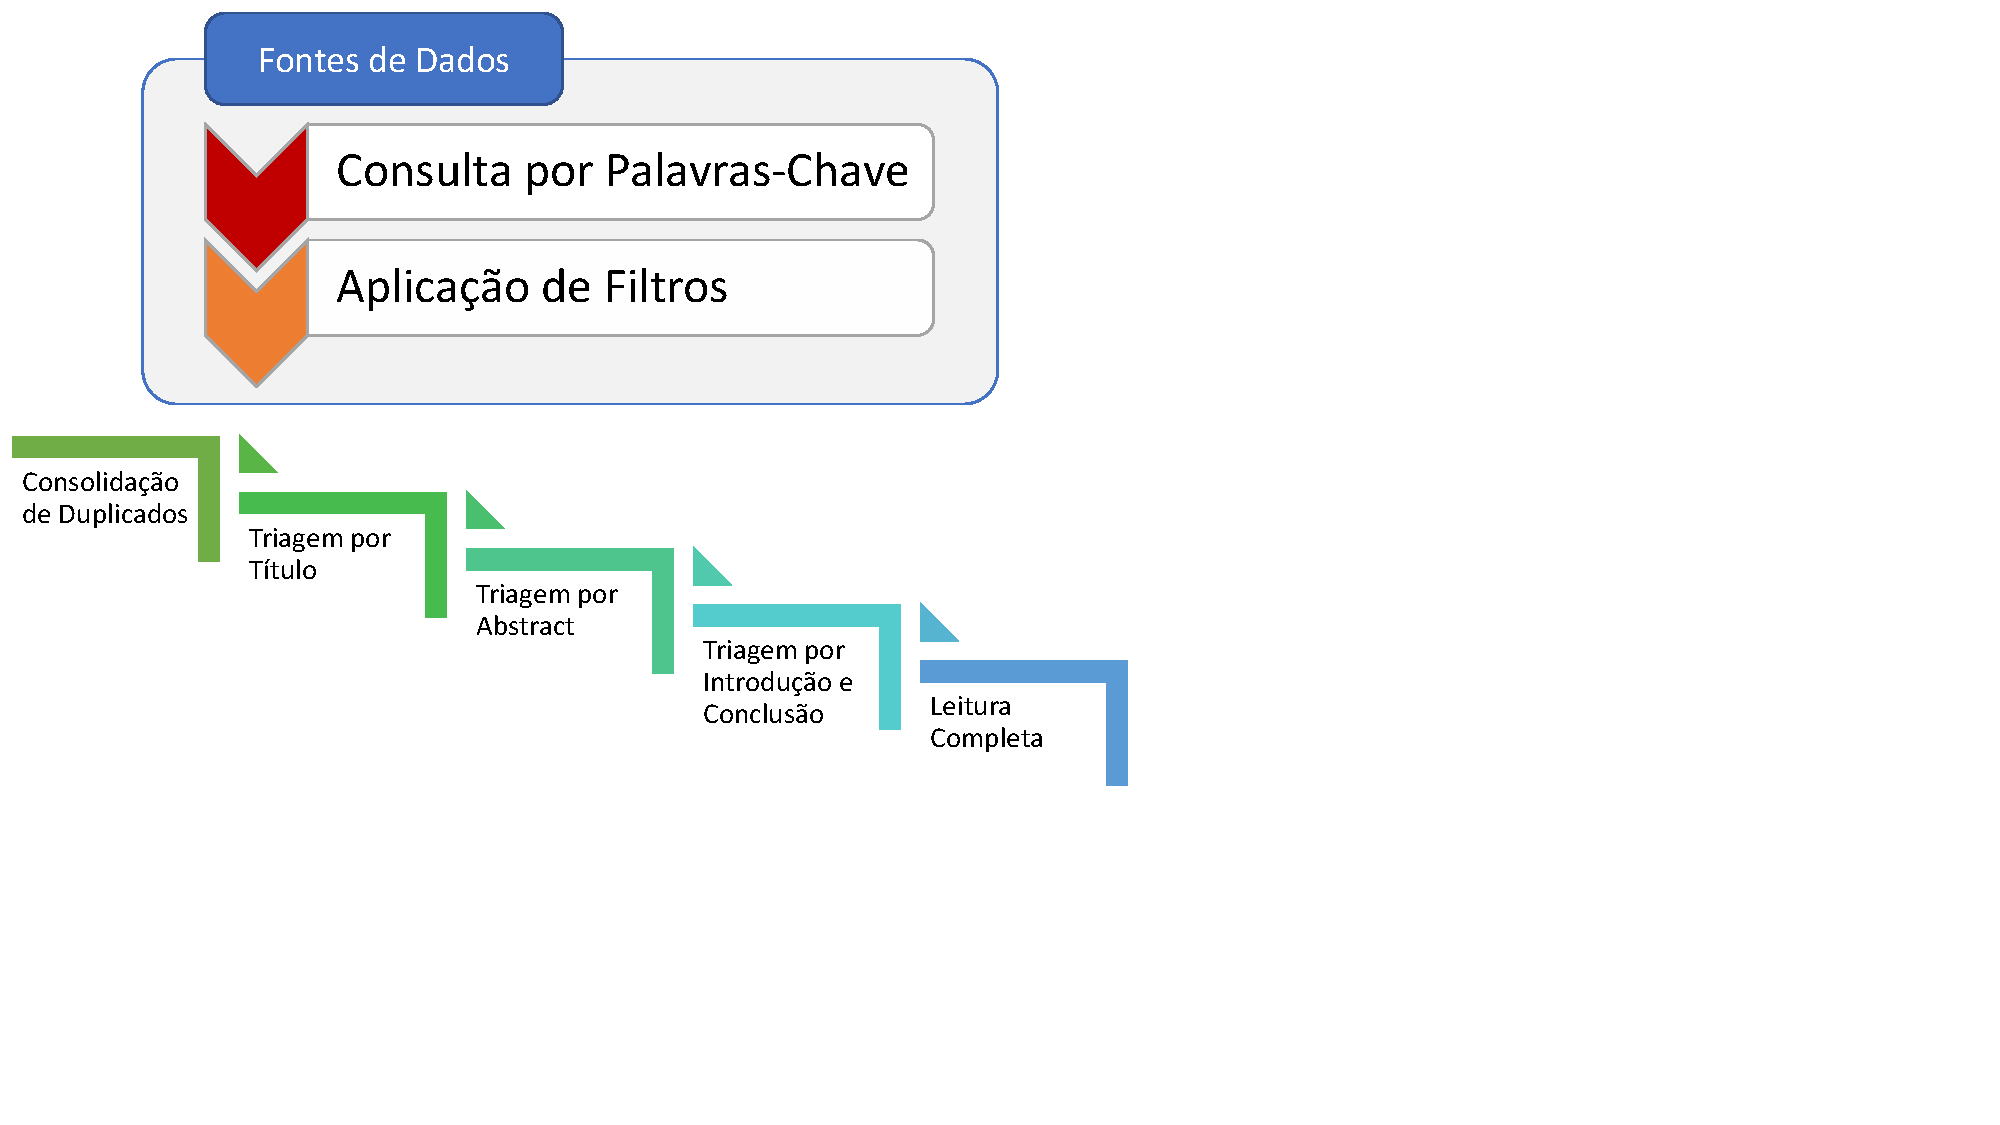
\includegraphics[trim=0 160 420 0,clip,width=\textwidth]{survey-pipeline}
	\fonte{Elaborado pelo autor.}
\end{minipage}
\end{figure}


Diante destas dificuldades e o volume de artigos encontrados em estágios iniciais da abordagem sistemática\footnote{
	Utilizando-se dos bancos de dados disponíveis para a biblioteca da UNISINOS foram encontrados cerca de 7500 artigos no primeiro estágio do mapeamento sistemático utilizando o termo de busca \texttt{(phylogeny OR phylogenetics OR phylogenetic) AND (software OR tool OR program OR package)}, adicionalmente aos filtros: somente resultados que contemplem texto completo disponível, publicados em revistas com revisão por pares, datados a partir de 1990 e com idioma inglês.
}, a estratégia para o mapeamento do estado da arte passou a ser uma revisão de literatura.
Apesar da mudança na estratégia do levantamento, boa parte dos passos anteriores seguiram relevantes, dentre eles, o estabelecimento das questões de pesquisa, das palavras-chaves e dos demais filtros, apresentados a seguir.
Buscou-se com este trabalho encontrar o estado da arte situado na intersecção entre computação de alto desempenho e bioinformática, mais precisamente estudos filogenéticos, o que resultou nas seguintes questões de pesquisa:


\begin{enumerate}[label=Questão~\arabic*:,itemindent=*]
	
	%\item Quais são os softwares mais avançados para inferência filogenética disponíveis hoje?
	
	\item Quais técnicas de otimização são usadas atualmente para possibilitar a inferência de grandes filogenias?
	
	\item Qual é o cenário no que diz respeito a adoção de técnicas de computação paralela e distribuída para inferência filogenética?
	
	\item Quais são os desafios encontrados pelos autores e as oportunidades disponíveis para avançar o estado da arte no que diz respeito a computação paralela e distribuída aplicada à algoritmos filogenéticos?
	
\end{enumerate}


Uma vez definidas as questões de pesquisa, o próximo passo para a execução do mapeamento consiste em estabelecer as palavras-chaves mais apropriadas para esta pesquisa, além de definir filtros adicionais, também chamados de critérios de inclusão, afim de aprimorar a qualidade dos resultados e formular a \textit{string} de busca.


No que diz respeito às palavras-chaves foram definidos três termos fundamentais e dois opcionais, demonstrados na \autoref{tab:survey-keywords}.
A existência de termos opcionais mostrou-se necessária em função da grande variação entre as diferentes bases de dados, conforme abordado anteriormente nas dificuldades do mapeamento sistemático.
Os filtros detalhados na \autoref{tab:survey-filters} visam estabelecer critérios de qualidade a respeito do material utilizado neste mapeamento e seguem boas práticas, com a notável omissão de um limite quanto a data de publicação.
Esta ausência ocorre também em função das particularidades encontradas no mapeamento.


% ORDENADO POR RELEVÂNCIA OU CITAÇÕES 


A execução das buscas teve como objetivo a cobertura de um amplo leque de editoras especializadas em ciência da computação e bioinformática, como: \textit{Association for Computing Machinery} (ACM), \textit{Institute of Electrical and Electronics Engineers} (IEEE), \textit{BioMed Central} (BMC) e \textit{Public Library of Science} (PLOS), assim como veículos de ampla cobertura, como Elsevier, Nature e Springer, além de agregadores como o \textit{Google Scholar}, com a lista completa disponível na \autoref{tab:survey-sources}.


A elaboração das \textit{strings} de busca varia de acordo com as capacidades de cada plataforma, com preferência para formatos baseados em expressões booleanas compostas pela combinação das palavras-chaves básicas e opcionais por operadores de conjunção lógica (E) incluindo termos sinônimos em operadores de disjunção, por exemplo:
\begin{verbatim}
    (phylogeny OR phylogenetics OR phylogenetic) 
AND (software OR tool OR program OR package) 
AND (inference) 
AND (cloud)
\end{verbatim}
Em casos nos quais a busca resultava em poucos ou nenhum resultado, as palavras-chaves opcionais eram removidas da expressão.
Já a aplicação dos filtros era realizada na própria plataforma de busca, quando esta fornecia tais capacidades ou realizada de maneira manual, caso contrário.


%
%No início da pesquisa foram encontrados 694 trabalhos e após as etapas de remoção de impurezas conforme
%os critérios supracitados, remoção de artigos duplicados, filtro por título, filtro por abstract, filtro por introdução e
%filtro por leitura completa, chegamos aos 24 artigos selecionados,


As próximas etapas do levantamento bibliográfico consistiram na avaliação manual de cada resultado para garantir sua relevância no contexto deste trabalho, em consonância com suas questões de pesquisa.
Para tanto, adotou-se uma abordagem estruturada, conforme \autoref{fig:survey-pipeline}, que compôs o \textit{pipeline} de seleção, composta pelos seguintes passos:
\begin{inparaenum}[I)]
	\item aplicação dos filtros (caso necessário);
	\item consolidação de duplicados;
	\item triagem baseada no título;
	\item triagem baseada no abstract;
	\item triagem por leitura da introdução e conclusão; e 
	\item triagem por leitura completa.
\end{inparaenum}


%jmodeltest.org (é "cloud" mas não menciona elasticidade) \cite{DarribaPHD}

% Keane2006a !!!


\section{Taxonomia Elaborada}
\label{sec:taxonomia}


\begin{figure}[tb]
	\centering%
	\begin{minipage}{\defaultFigureWidth\textwidth}
		\caption{Taxonomia elaborada para a classificação dos trabalhos identificados durante a etapa de revisão de literatura.}
		\label{fig:taxonomia}
		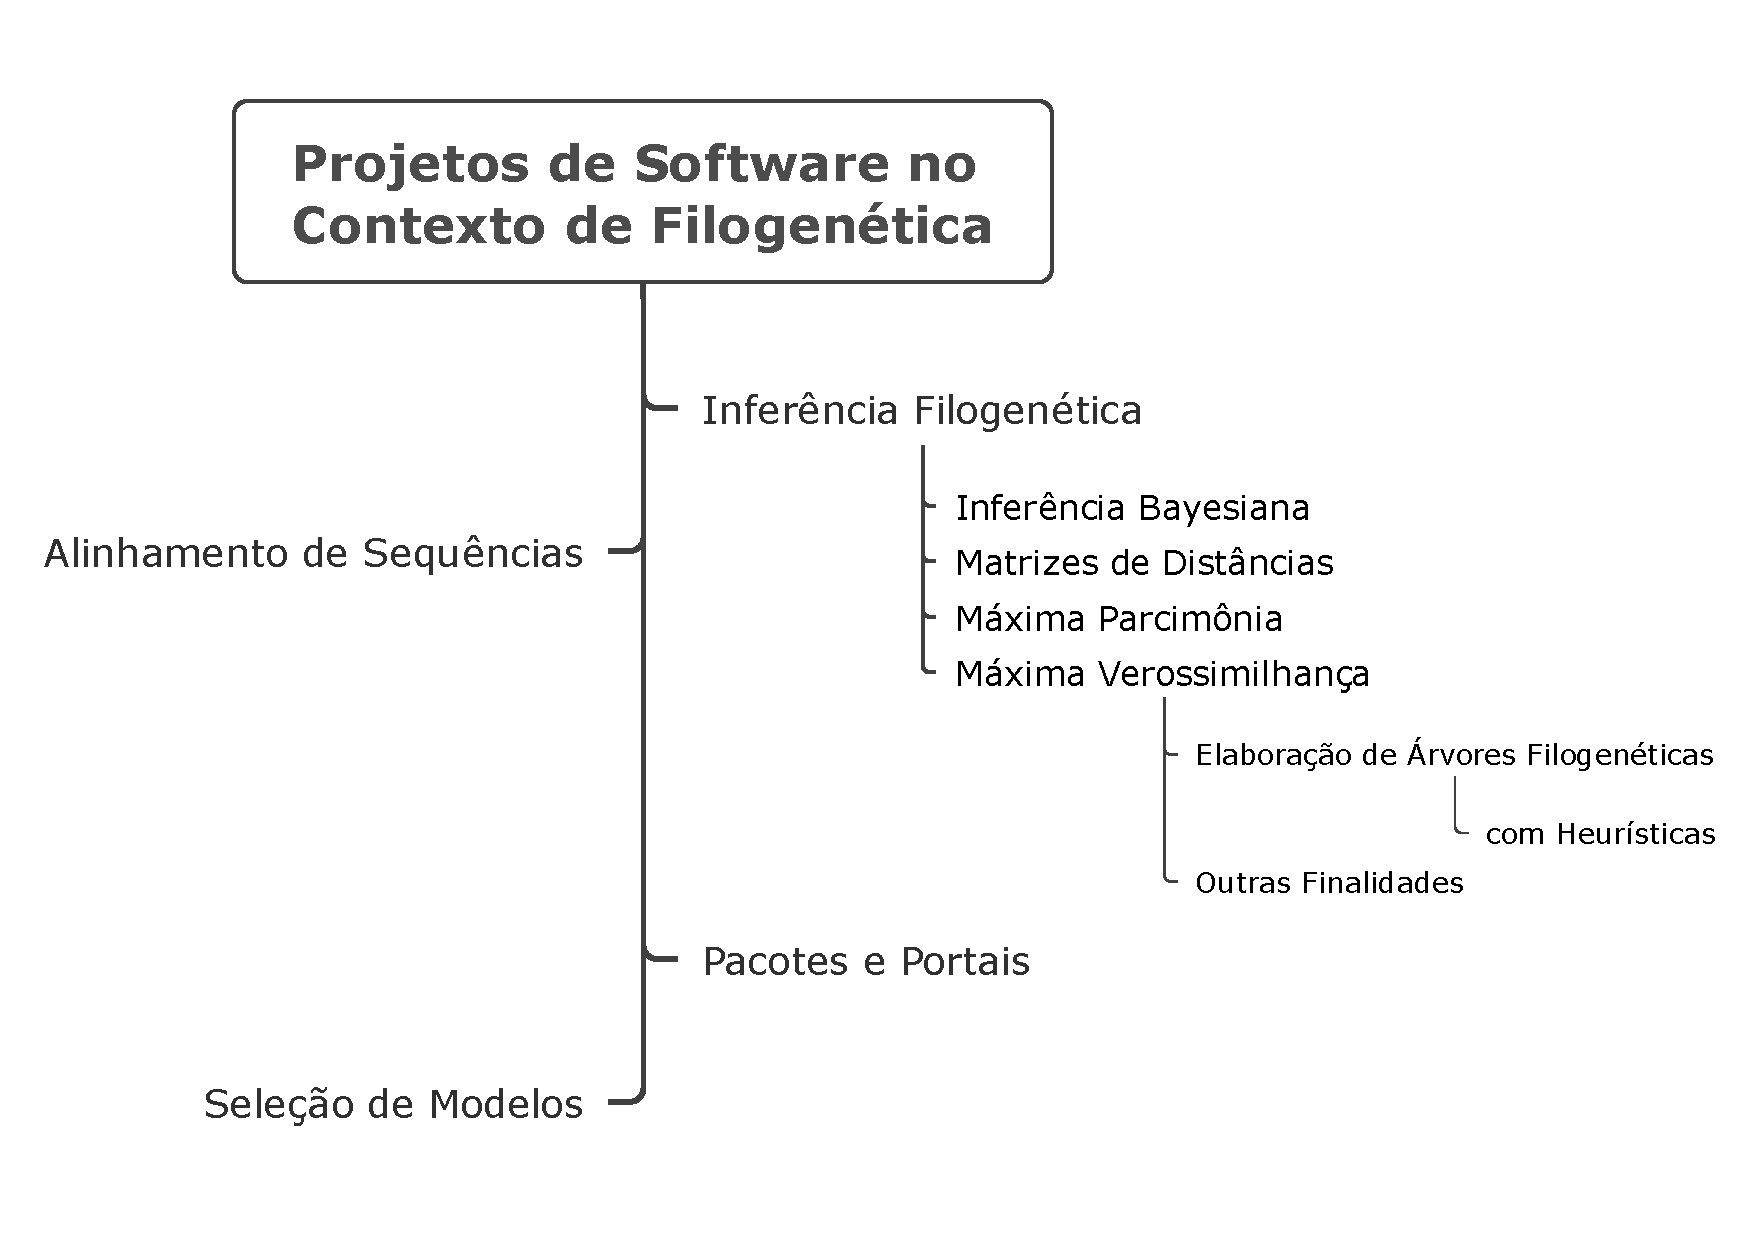
\includegraphics[trim=15 40 15 40,clip,width=\textwidth]{taxonomia}
		\fonte{Elaborado pelo autor.}
	\end{minipage}
\end{figure}


Ao analisar o corpo de dados obtido através do levantamento bibliográfico, o objetivo é responder às questões de pesquisa previamente estabelecidas.
Contudo, devido à amplitude da área de conhecimento e ao elevado número de resultados, a elaboração de uma taxonomia que se proponha a ajudar na classificação, comparação e avaliação dentre os múltiplos projetos de software encontrados no campo da filogenética foi julgada relevante para o escopo desta dissertação assim como contribuição.


Embora muito se fale em taxonomias no contexto de filogenética, estas se referem, sua grande maioria, à descrição, denominação e classificação de organismos vivos~\cite{yang2014molecular}, não devendo ser confundida com a proposta deste trabalho.
%
O objetivo buscado aqui consiste em uma abordagem hierárquica capaz de representar um corpo de conhecimento de um determinado campo de estudo e que também pode ser visualizado como uma árvore~\cite{Denning2009}.
%
Adicionalmente, as pesquisas realizadas durante o levantamento bibliográfico não contemplavam qualquer tipo de estrutura formal dos projetos de computação aplicados à filogenética, de maneira que a taxonomia aqui proposta pode ser considerada um esforço inicial neste sentido.


No entanto, ao invés de construir uma taxonomia teórica e então aplicá--la na classificação de projetos existentes, foi adotada uma abordagem prática: construção  da taxonomia com base nos resultados obtidos através do levantamento bibliográfico e, assim como~\cite{Perera2013}, identificando características, técnicas, funcionalidades ou abordagens empregadas pelos projetos de software contemplados no levantamento.
Tal abordagem é relevante uma vez que, para o melhor do conhecimento do autor, não foram encontradas nenhuma outra taxonomia ou classificação similar que contemplasse a intersecção entre filogenética e bioinformática com a computação de alto desempenho.


Diante desta situação, e conforme pode ser visto na \autoref{fig:taxonomia}, foi formalizada uma taxonomia que classifica os trabalhos encontrados em distintas categorias e em uma estrutura hierárquica que contempla as principais características de cada trabalho.
Esta taxonomia pode ser dividida em quatro pilares principais:
\begin{inparaenum}[\itshape a\upshape)] 
	\item Inferência Filogenética;
	\item Pacotes e Portais;
	\item Seleção de Modelos de Substituição Molecular; e
	\item Alinhamento de Sequências Moleculares.
\end{inparaenum}


Ademais, o pilar que trata de inferência filogenética foi adicionalmente dividido em termos dos métodos utilizados e de suas finalidades, de acordo com os conceitos apresentados na \autoref{s:phylogeneticinference}.
Estatísticas quanto ao número de trabalhos encontrados para cada nível da taxonomia são encontradas na \autoref{tab:survey-stats-bio}.




\section{Análise do Estado da Arte}
\label{sec:analise-estadodaarte}

%TXDO: Eu desenvolveria um pouco mais o 3.2, com a ideia de ter pelo menos umas 3 ou 4 frases sobre cada trabalho, e aglutinando aqueles que falaram a mesma coisa.


\begin{table}[tb]
	%\small
	\centering%
	\begin{minipage}{\defaultFigureWidth\textwidth}
		\caption{Quantidade de trabalhos da revisão de literatura quando classificados conforme as categorias presentes na taxonomia
			proposta}
		\label{tab:survey-stats-bio}
		\vspace{1ex}
		\centering
		\begin{tabulary}{\textwidth}{LLLlr@{}}
			\toprule
			Categoria	& Método	& \multicolumn{2}{l}{Finalidade}	& Quantidade \\
			\midrule
			\multirow{6}{6em}{Inferência Filogenética} & \multirow{3}{7em}{Máxima Verossimilhança} & \multicolumn{2}{l}{~~Outras Finalidades}	& 22	\\ \cmidrule(l){3-5}
			&	& ~~\multirow{2}{6em}{Elaboração \\ de Árvores Filogenéticas} &	& 17 \\ \cmidrule(l){4-5}
			&	&	& ~~com Heurísticas & 5	\\ \cmidrule(l){2-5}
			& \multicolumn{3}{l}{~~Inferência Bayesiana}	& 3 \\ \cmidrule(l){2-5}
			& \multicolumn{3}{l}{~~Matrizes de Distâncias}	& 3 \\ \cmidrule(l){2-5}
			& \multicolumn{3}{l}{~~Máxima Parcimônia}	& 2 \\ \midrule
			\multicolumn{4}{l}{Pacotes e Portais}	& 17 \\ \midrule
			\multicolumn{4}{l}{Seleção de Sistemas}	& 10 \\ \midrule
			\multicolumn{4}{l}{Alinhamento de Sequências}	& 4 \\
			\bottomrule
			\multicolumn{4}{r}{\textbf{Total}} & \textbf{83}
		\end{tabulary}
		\fonte{Elaborado pelo autor.}
	\end{minipage}
\end{table}




Uma vez executado o levantamento previamente descrito, apresenta-se, nesta seção, a lista de trabalhos selecionados para análise do estado da arte.
Ao todo foram encontrados 83 trabalhos relevantes, todos eles situados na intersecção entre inferência filogenética e a ciência da computação, contemplando temas como:
\begin{inparaenum}[\itshape a\upshape)] 
	\item Alinhamento de Sequências Moleculares;
	\item Seleção de Sistemas de Substituição Molecular;
	\item Pacotes e Portais; e
	\item Inferência Filogenética.
\end{inparaenum}


%Em casos como este, onde existe uma grande variedade de temas encontrados dentre os resultados do levantamento bibliográfico, torna-se necessária uma categorização dos mesmos para que possam ser estabelecidos paralelos de comparação entre trabalhos relacionados.
%Diante desta situação, e conforme pode ser visto na \autoref{fig:taxonomia}, formalizou-se uma taxonomia que classifica os trabalhos encontrados em distintas categorias e em uma estrutura hierárquica que contempla as principais características de cada trabalho.
%Estatísticas quanto ao número de trabalhos encontrados para cada nível da taxonomia são encontradas na \autoref{tab:survey-stats-bio}.


Do ponto de vista da filogenética é interessante notar a grande quantidade de ferramentas disponíveis para inferência filogenética, contudo há uma notável predominância de softwares que utilizam métodos baseados em ML (\autoref{sub:bio-max-likelyhood}).
Outra estatística que se destaca é a grande quantidade de ferramentas classificadas como `Pacotes e Portais', categoria que contempla os trabalhos que não se limitam a um único método de inferência ou que também incluem funcionalidades das demais categorias.


Tais projetos buscam centralizar boa parte das tarefas envolvidas no processo de análise filogenética, sendo notáveis exemplos os projetos CIPRES \cite{Miller2010}, GALAXY \cite{Afgan2016}, MEGA \cite{Kumar2016}, e Phylemon \cite{Tarraga2007,Sanchez2011}.
Além de pacotes de software que moldaram os rumos da bioinformática no contexto da filogenética, como é o caso do PHYLIP de \citetexto{Felsenstein1989}, autor que consta na lista da revista Nature dos 100 mais citados \cite{NatureTop100}.


Em tratando-se de características computacionais, o objetivo desta pesquisa foi realizar um mapeamento das capacidades dos softwares no que diz respeito a computação paralela e distribuída e, principalmente, a elasticidade de recursos.
Desta forma, buscou-se nas publicações e, quando disponível, nas páginas e documentações dos projetos, informações que pudessem indicar o suporte à características como:


\begin{enumerate}[label=Característica~\arabic*:,itemindent=*]
	
	\item Suporte à diretivas de computação distribuída (excetuando-se paralelismo na própria máquina, através de processadores \textit{multi-core}, por exemplo);
	
	\item Suporte à elasticidade no consumo de recursos e, de maneira mais ampla, suporte a contextos de \textit{cloud computing};
	
	\item Implementação de diretivas para balanceamento de carga, seja no contexto de \textit{cloud} ou de computação distribuída;
	
	\item Suporte à computação baseada em placas gráficas, \textit{Graphics Processing Unit} (GPU), que costuma ser muito eficaz em contextos científicos;
	
	\item Modelo de interação com o usuário, caso o software suporte comandos interativos ou disponha de uma interface gráfica.
	
\end{enumerate}


\begin{table}[b]
\centering%
\begin{minipage}{\defaultFigureWidth\textwidth}
	\caption{Quantidade de trabalhos da revisão de literatura quando classificados de acordo com as características relevantes para a computação distribuída.}
	\label{tab:survey-stats-comp}
	\vspace{1ex}
	\setlength{\tymin}{3.5em}
		\begin{tabulary}{\textwidth}{@{}CCCCCCC@{}}
			\toprule
			\vspace{1ex}Projetos & Console Interativo & Interface Gráfica & Computação Distribuída & Aceleração por GPU & Elasticidade de Recursos & Balanceamento de Carga \\*
			\midrule
			\multirow{2}{*}{{\large 83}} & 45 & 34 & 19 & 4 & 3 & 2 \\* 
			%\cmidrule{2-7}
			\dashedline{2-7}
			& 54\% & 41\% & 23\% & 5\% & 4\% & 2\% \\*
			\bottomrule
		\end{tabulary}
	\fonte{Elaborado pelo autor.}%
\end{minipage}
\end{table}


De acordo com os critérios estabelecidos é possível montar um panorama do estado da arte no que diz respeito às ferramentas para filogenética inseridas no contexto de computação em nuvem e elasticidade, sumarizado na \autoref{tab:survey-stats-comp}.
Apesar do amplo suporte à interfaces gráficas ou consoles interativos, presente em praticamente 60\% dos softwares encontrados, apenas 23\% deles incluem algum tipo de suporte à computação distribuída, sendo fornecido, na grande maioria dos casos, por implementações baseadas em \textit{Message Passing Interface} (MPI), com o projeto TNT, por \citetexto{Goloboff2016}, destacando-se como a única exceção encontrada ao trabalhar com \textit{Parallel Virtual Machine} (PVM), um predecessor do MPI.


Em tratando-se de técnicas mais recentes, como a computação baseada em GPU, apenas quatro trabalhos alegam suporte, sendo eles:
\begin{inparaenum}[\itshape a\upshape)]
	\item o projeto GALAXY \cite{Afgan2016} através de seus \textit{plug--ins};
	\item os softwares BEAST \cite{Drummond2002} e mrBayes \cite{Huelsenbeck2001}, que aceleram na GPU as computações do algoritmo Metropolis-Hastings, também conhecido como Markov chain Monte Carlo (MCMC); e
	\item METAPIGA \cite{Helaers2010} completa a lista, tirando proveito da GPU para executar uma heurística para a inferência filogenética baseada em algoritmos genéticos.
\end{inparaenum}


No campo da elasticidade de recursos e da computação em nuvem a situação é agravada, com apenas três dos trabalhos anunciando suporte.
Apesar de portais como CIPRES \cite{Miller2010}, Phylemon \cite{Tarraga2007,Sanchez2011} e Phylogeny.fr \cite{Dereeper2008} alegarem elasticidade, não foram encontrados indícios de suporte à nível de algoritmo, sendo a elasticidade, nestes casos, referente à capacidade de adequar os recursos consumidos ao volume de usuários ativos nas plataformas, também é importante notar a abstenção de suporte à elasticidade automática, com ajustes ficando a cargo dos operadores dos portais supracitados, o que na opinião do autor anula os benefícios de um ambiente baseado na computação em nuvem.


Merecem destaque no que diz respeito a elasticidade de recursos os trabalhos de \citetexto{Keane2005} e \citetexto{Keane2007} que através dos projetos DPRML e, posteriormente, MultiPhyl apresentam uma plataforma de inferência filogenética nos moldes de projetos como Folding@home \cite{Shirts2000,Larson2002} e SETI@home \cite{Korpela2001}, utilizando recursos ociosos de computadores pessoais.
Apesar de não figurar explicitamente como computação em nuvem, devido ao uso de computadores das universidades ao invés de provedores como \textit{Amazon Web Services} (AWS), Azure ou Google Cloud, projetos como estes enfrentam os mesmos desafios técnicos, do ponto de vista da elasticidade, de um projeto \textit{cloud native}.
Completa a lista o portal GALAXY \cite{Afgan2016}, ao fornecer, através dos seus \textit{add--ons} algoritmos que tiram proveito de ambientes de nuvem, além de oferecer imagens compatíveis com provedores como AWS \cite{Varia2017}, OpenStack \cite{Sefraoui2012} e OpenNebula \cite{Milojicic2011}.
Tais imagens carregam todos os componentes do software empacotados e configurados para se beneficiar ao máximo da elasticidade presente nestes contextos, facilitando a gestão e configuração dos ambientes.


Afim de apresentar uma visão consolidada entre os temas abordados nesta seção elaborou-se a \autoref{tab:survey-comparativo}, que combina as características relevantes para a filogenética e a bioinformática, oriundas da taxonomia apresentada na \autoref{fig:taxonomia}, com os atributos mais relevantes para a computação distribuída conforme elencados na \autoref{tab:survey-stats-comp}.
Ao conciliar os dados referentes a estes dois pontos de vista, filogenético e da computação distribuída, chegou-se, enfim, ao estado da arte em termos de produção bibliográfica pertencente a esta intersecção, possibilitando, em última análise, a identificação de pontos fortes e fracos desta área do conhecimento, sendo estes pontos fracos o objetivo de estudo da próxima seção.




\section{Lacunas de Pesquisa}
\label{sec:lacunas-de-pesquisa}


\begin{figure}[tb]
	\centering%
	\begin{minipage}{\defaultFigureWidth\textwidth}
		\caption{Comparativo entre a evolução do poder computacional das CPUs versus GPUs medido em GFLOP/s.}
		\label{fig:gpu-power}
		\vspace{1ex}
		\includegraphics[trim=105 170 70 395,clip,width=\textwidth]{nvidia}
		\fonte{\citetexto{nvidia2018}.}
	\end{minipage}
\end{figure}

De posse do estado da arte e compreendendo melhor o contexto em que se inserem as ferramentas computacionais utilizadas na filogenética, pode-se encontrar pontos de melhoria e novas abordagens capazes de, entre outros, acelerar o processamento de dados e a quantidade de amostras, aumentando a eficiência dos programas e dos pesquisadores da bioinformática e contribuindo, em última instância, ao avanço na qualidade da produção científica.
Motivados por este objetivo e munidos de conhecimentos oriundos da computação paralela e distribuída \cite{Righi2013,Aubin2016,Aubin2017} 
foram identificadas três lacunas de pesquisa no contexto deste trabalho, nomeadamente: 
\begin{enumerate}[label=Lacuna~\arabic*:~,itemindent=*]
	\item Aceleração por GPUs;
	\item Balanceamento de carga;
	\item Elasticidade na utilização de recursos.
\end{enumerate}


% GPU


Apesar do foco de investimentos em melhorias na capacidade computacional tenha permanecido por muitos anos na CPU, este cenário já não é o mesmo atualmente, com as GPUs ganhando relevância em termos de poder computacional aliado a um custo atrativo.
Conforme pode ser visto na \autoref{fig:gpu-power}, GPUs já estão muito a frente no que diz respeito ao poder bruto de processamento, sendo especialmente relevantes para contextos científicos \cite{Aji2013}.
Dada a natureza dos cálculos de inferência filogenética, a aplicação de GPUs se apresenta como uma ótima combinação haja vista que o alto grau de paralelismo permite explorar, em múltiplas frentes de simulação, o espaço de busca da melhor árvore filogenética que representa os dados de entrada.
Um problema similar é a descida de gradientes aplicada na área da Inteligência Artificial (IA) e que já tira proveito da GPU para tal, vide \citetexto{Zhang2013}.


% Load Balancing


Ainda que quase um quarto dos softwares analisados disponham de iniciativas que apoiam a computação distribuída, poucos foram aqueles que mencionaram estratégias de balanceamento de carga entre seus atributos técnicos.
Embora não seja estritamente necessário para obter acesso às melhorias de performance oriundas da computação distribuída, a aplicação de balanceamento de carga assegura um melhor aproveitamento dos recursos disponíveis, aumentando a eficiência e potencialmente reduzindo ainda mais o tempo de execução.
Através de revisões como a apresentada por \citetexto{Mishra2018}, foram encontradas diversas sugestões de algoritmos e estratégias para balanceamento de carga, muitas das quais certamente poderiam ser aplicadas com resultados positivos neste contexto.


% Elasticidade


Outra abordagem com baixa penetração dentre os projetos encontrados é a elasticidade de recursos, abordada na \autoref{sec:elasticidade}, característica que permite ao software se ajustar a quantidade de recursos disponível de maneira dinâmica, seja para mais ou para menos, sem que seja necessário interromper sua execução.
Menção honrosa neste sentido são os trabalhos de \citetexto{Keane2005} e \citetexto{Keane2007}, que tornaram os projetos DPRML e MultiPhyl aptos a trabalharem com recursos variáveis ainda que sem estar inserido em um contexto de computação em nuvem.
Especulou-se que a baixa adoção a estratégias de elasticidade deve-se em parte ao modelo de investimento onde instituições investem os recursos oriundos dos financiamentos e bolsas em \textit{clusters}, e estes são renovados periodicamente de maneira que o modelo de uso está sempre baseado na substituição, ao invés da complementação, através da adição de novos recursos.
Contudo, acredita-se que os incentivos financeiros a adoção da elasticidade, aliados à maior participação dos provedores de computação em nuvem no meio acadêmico, farão com que aumente a relevância de projetos já preparados a tirar proveito destas capacidades.




\afterpage{%
	%config ONESIDE
	%\newgeometry{inner=1.75cm}
	
	%config TWOSIDE
	%\newgeometry{inner=2cm,centering,bindingoffset=0pt}
	\newgeometry{textheight=108ex}
	\setlength{\oddsidemargin}{-8mm}
	\setlength{\evensidemargin}{-8mm}
	
	
	%padrão daqui pra baixo
	
	\clearpage	% Flush earlier floats
	\scriptsize
	\centering
	
	\newlength{\atributowidth}
	\setlength{\atributowidth}{4.5em}
	\newcommand\tabelaosectionindent{1.25em}
	\newcommand\tabelaocaption{Comparativo entre trabalhos encontrados na revisão de literatura classificados de acordo com a taxonomia proposta e atributos de interesse}
	
	\begin{longtabu} to 1.1\textwidth[c]{llp{\atributowidth}p{\atributowidth}p{\atributowidth}p{\atributowidth}p{\atributowidth}p{\atributowidth}}
		
		\multicolumn{8}{@{}r@{}}{Tabela~\thetable~-- \tabelaocaption}
		\addcontentsline{lot}{table}{\protect\numberline{\thetable}{\tabelaocaption}}
		\label{tab:survey-comparativo}
		\\*[-1ex]
		\multicolumn{8}{r@{}}{{(continua)}} \\*
		\toprule
		\multicolumn{1}{c}{\multirow{3}{*}{Projeto}} & \multicolumn{1}{c}{\multirow{3}{*}{Citação}} & \multicolumn{6}{c}{Atributo} \\*
		\cmidrule{3-8}
		& & Con\-so\-le In\-te\-ra\-ti\-vo & In\-ter\-fa\-ce Grá\-fi\-ca & Com\-pu\-ta\-ção Dis\-tri\-bu\-í\-da & A\-ce\-le\-ra\-ção por GPU & E\-las\-ti\-ci\-da\-de de Re\-cur\-sos & Ba\-lan\-ce\-a\-men\-to de Car\-ga \\*
		\midrule
		\endfirsthead
		%
		\multicolumn{8}{@{}r@{}}{Tabela~\thetable~-- \tabelaocaption}
		\\*[-1ex]
		\multicolumn{8}{r@{}}{{(continuação)}} \\*
		\toprule
		\multicolumn{1}{c}{\multirow{3}{*}{Projeto}} & \multicolumn{1}{c}{\multirow{3}{*}{Citação}} & \multicolumn{6}{c}{Atributo} \\*
		\cmidrule{3-8} 
		& & Con\-so\-le In\-te\-ra\-ti\-vo & In\-ter\-fa\-ce Grá\-fi\-ca & Com\-pu\-ta\-ção Dis\-tri\-bu\-í\-da & A\-ce\-le\-ra\-ção por GPU & E\-las\-ti\-ci\-da\-de de Re\-cur\-sos & Ba\-lan\-ce\-a\-men\-to de Car\-ga \\*
		\midrule
		\endhead
		%
		
		\bottomrule
		\endfoot
		%
		
		\bottomrule
		\multicolumn{2}{r}{\textbf{Totais}} & \multicolumn{1}{c}{\textbf{45}} & \multicolumn{1}{c}{\textbf{34}} & \multicolumn{1}{c}{\textbf{19}} & \multicolumn{1}{c}{\textbf{4}} & \multicolumn{1}{c}{\textbf{3}} & \multicolumn{1}{c}{\textbf{2}} \\*
		\multicolumn{8}{l}{Fonte:~Elaborado pelo autor.} \\*
		\endlastfoot
		%
		
		\multicolumn{8}{l}{\hspace{\tabelaosectionindent}\textbf{\textit{
					Alinhamento de Sequências Moleculares}}} \\*
		
		Clustal Omega & \citetexto{Sievers2014} &  &  &  &  &  &  \\
		MUSCLE & \citetexto{Edgar2004} &  &  &  &  &  &  \\
		segminator & \citetexto{Archer2010} & \multicolumn{1}{c}{\checked} & \multicolumn{1}{c}{\checked} &  &  &  &  \\
		T-Coffee & \citetexto{Notredame2000} &  &  &  &  &  &  \\
		
		
		
		\multicolumn{8}{l}{\hspace{\tabelaosectionindent}\textbf{\textit{
					Seleção de Sistemas de Substituição}}} \\*
		
		CoMET & \citetexto{Lee2006} & \multicolumn{1}{c}{\checked} & \multicolumn{1}{c}{\checked} &  &  &  &  \\
		Concaterpillar & \citetexto{Leigh2008} &  &  & \multicolumn{1}{c}{\checked} &  &  &  \\
		DTModSel & \citetexto{Minin2003} &  &  &  &  &  &  \\
		jmodeltest & \citetexto{Posada2008} & \multicolumn{1}{c}{\checked} & \multicolumn{1}{c}{\checked} &  &  &  &  \\
		jmodeltest2 & \citetexto{Darriba2012} & \multicolumn{1}{c}{\checked} & \multicolumn{1}{c}{\checked} & \multicolumn{1}{c}{\checked} &  &  &  \\
		kakusan & \citetexto{Tanabe2011} & \multicolumn{1}{c}{\checked} &  &  &  &  &  \\
		modelgenerator & \citetexto{Keane2006} &  &  &  &  &  &  \\
		modeltest & \citetexto{Posada1998} &  &  &  &  &  &  \\
		MrModeltest  & \citetexto{Nylander2004} &  &  &  &  &  &  \\
		ProtTest & \citetexto{Abascal2005} & \multicolumn{1}{c}{\checked} & \multicolumn{1}{c}{\checked} & \multicolumn{1}{c}{\checked} &  &  &  \\
		
		
		
		\multicolumn{8}{l}{\hspace{\tabelaosectionindent}\textbf{\textit{
					Pacotes e Portais}}} \\*
		
		ARB & \citetexto{Ludwig2004} & \multicolumn{1}{c}{\checked} & \multicolumn{1}{c}{\checked} &  &  &  &  \\
		Bio++ & \citetexto{Dutheil2006} &  &  &  &  &  &  \\
		BOSQUE & \citetexto{Ramirez-Flandes2008} & \multicolumn{1}{c}{\checked} & \multicolumn{1}{c}{\checked} &  &  &  &  \\
		CIPRES & \citetexto{Miller2010} &  & \multicolumn{1}{c}{\checked} & \multicolumn{1}{c}{\checked} &  &  &  \\
		DAMBE & \citetexto{Xia2017} & \multicolumn{1}{c}{\checked} & \multicolumn{1}{c}{\checked} &  &  &  &  \\
		EMBOSS & \citetexto{Rice2000} & \multicolumn{1}{c}{\checked} &  &  &  &  &  \\
		GALAXY & \citetexto{Afgan2016} & \multicolumn{1}{c}{\checked} & \multicolumn{1}{c}{\checked} & \multicolumn{1}{c}{\checked} & \multicolumn{1}{c}{\checked} & \multicolumn{1}{c}{\checked} &  \\
		MEGA & \citetexto{Kumar2016} & \multicolumn{1}{c}{\checked} & \multicolumn{1}{c}{\checked} &  &  &  &  \\
		mesquite & \citetexto{Maddison2015} & \multicolumn{1}{c}{\checked} & \multicolumn{1}{c}{\checked} &  &  &  &  \\
		PAL & \citetexto{Drummond2001} &  &  &  &  &  &  \\
		paup* & \citetexto{Swofford2002} & \multicolumn{1}{c}{\checked} & \multicolumn{1}{c}{\checked} &  &  &  &  \\
		Phylemon & \citetexto{Tarraga2007} & \multicolumn{1}{c}{\checked} & \multicolumn{1}{c}{\checked} &  &  &  &  \\
		Phylemon 2.0 & \citetexto{Sanchez2011} & \multicolumn{1}{c}{\checked} & \multicolumn{1}{c}{\checked} &  &  &  &  \\
		PHYLIP & \citetexto{Felsenstein1989} & \multicolumn{1}{c}{\checked} &  &  &  &  &  \\
		phylo\_win & \citetexto{Galtier1996} & \multicolumn{1}{c}{\checked} & \multicolumn{1}{c}{\checked} &  &  &  &  \\
		Phylogeny.fr & \citetexto{Dereeper2008} &  & \multicolumn{1}{c}{\checked} &  &  &  &  \\
		SeaView & \citetexto{Gouy2010} & \multicolumn{1}{c}{\checked} & \multicolumn{1}{c}{\checked} &  &  &  &  \\
		
		
		
		\multicolumn{8}{l}{\hspace{\tabelaosectionindent}\textbf{\textit{
					Inferência Filogenética por Inferência Bayesiana}}} \\*
		
		BEAST & \citetexto{Drummond2002} & \multicolumn{1}{c}{\checked} & \multicolumn{1}{c}{\checked} &  & \multicolumn{1}{c}{\checked} &  &  \\
		mrBayes & \citetexto{Huelsenbeck2001} & \multicolumn{1}{c}{\checked} &  & \multicolumn{1}{c}{\checked} & \multicolumn{1}{c}{\checked} &  &  \\
		PhyloBayes & \citetexto{Lartillot2004} &  &  &  &  &  &  \\
		
		
		
		\multicolumn{8}{l}{\hspace{\tabelaosectionindent}\textbf{\textit{
					Inferência Filogenética por Matrizes de Distâncias}}} \\*
		
		BioNJ & \citetexto{Gascuel1997} & \multicolumn{1}{c}{\checked} &  &  &  &  &  \\
		QuickTree & \citetexto{Howe2002} &  &  &  &  &  &  \\
		TreeFit & \citetexto{Kalinowski2009} & \multicolumn{1}{c}{\checked} & \multicolumn{1}{c}{\checked} &  &  &  &  \\
		
		
		
		\multicolumn{8}{l}{\hspace{\tabelaosectionindent}\textbf{\textit{
					Inferência Filogenética por Máxima Parcimônia}}} \\*
		
		PhyloNET & \citetexto{Than2008} &  &  &  &  &  &  \\
		TNT & \citetexto{Goloboff2016} & \multicolumn{1}{c}{\checked} & \multicolumn{1}{c}{\checked} & \multicolumn{1}{c}{\checked} &  &  &  \\
		
		
		
		\multicolumn{8}{l}{\hspace{\tabelaosectionindent}\textbf{\textit{
					Inferência Filogenética por Máxima Verossimilhança focada em Elaboração de Árvores Filogenéticas}}} \\*
		
		ALIFRITZ & \citetexto{Fleissner2005} &  &  &  &  &  &  \\
		DNAML  & \citetexto{Felsenstein1996} & \multicolumn{1}{c}{\checked} &  &  &  &  &  \\
		DPRML & \citetexto{Keane2005} & \multicolumn{1}{c}{\checked} & \multicolumn{1}{c}{\checked} & \multicolumn{1}{c}{\checked} &  & \multicolumn{1}{c}{\checked} & \multicolumn{1}{c}{\checked} \\
		fastDNAml & \citetexto{Olsen1994} & \multicolumn{1}{c}{\checked} &  & \multicolumn{1}{c}{\checked} &  &  &  \\
		fasttree & \citetexto{Price2009} &  &  & \multicolumn{1}{c}{\checked} &  &  &  \\
		IQPNNI & \citetexto{Vinh2004} & \multicolumn{1}{c}{\checked} &  & \multicolumn{1}{c}{\checked} &  &  &  \\
		IQ-TREE & \citetexto{Nguyen2015} &  &  & \multicolumn{1}{c}{\checked} &  &  &  \\
		MultiPhyl & \citetexto{Keane2007} &  &  & \multicolumn{1}{c}{\checked} &  & \multicolumn{1}{c}{\checked} & \multicolumn{1}{c}{\checked} \\
		nhPhyML & \citetexto{Boussau2006} & \multicolumn{1}{c}{\checked} &  &  &  &  &  \\
		PhyML & \citetexto{Guindon2010} & \multicolumn{1}{c}{\checked} &  & \multicolumn{1}{c}{\checked} &  &  &  \\
		PHYML-aLRT & \citetexto{Anisimova2006} & \multicolumn{1}{c}{\checked} &  &  &  &  &  \\
		PhyML-Multi & \citetexto{Boussau2009} & \multicolumn{1}{c}{\checked} &  &  &  &  &  \\
		PROCOV & \citetexto{Wang2007} &  &  &  &  &  &  \\
		RAxML & \citetexto{Stamatakis2014} &  & \multicolumn{1}{c}{\checked} & \multicolumn{1}{c}{\checked} &  &  &  \\
		splitstree & \citetexto{Huson2006} & \multicolumn{1}{c}{\checked} & \multicolumn{1}{c}{\checked} &  &  &  &  \\
		treefinder & \citetexto{Jobb2004} & \multicolumn{1}{c}{\checked} & \multicolumn{1}{c}{\checked} &  &  &  &  \\
		tree-puzzle & \citetexto{Schmidt2002} & \multicolumn{1}{c}{\checked} &  & \multicolumn{1}{c}{\checked} &  &  &  \\
		
		
		
		\multicolumn{8}{l}{\hspace{\tabelaosectionindent}\textbf{\textit{
					Inferência Filogenética por Máxima Verossimilhança focada em Elaboração de Árvores Filogenéticas utilizando Heurísticas}}} \\*
		
		GARLI & \citetexto{Zwickl2006} &  &  & \multicolumn{1}{c}{\checked} &  &  &  \\
		METAPIGA & \citetexto{Helaers2010} & \multicolumn{1}{c}{\checked} & \multicolumn{1}{c}{\checked} & \multicolumn{1}{c}{\checked} & \multicolumn{1}{c}{\checked} &  &  \\
		PhyloCoco & \citetexto{Catanzaro2008} & \multicolumn{1}{c}{\checked} & \multicolumn{1}{c}{\checked} &  &  &  &  \\
		SEMPHY & \citetexto{Friedman2002} &  &  &  &  &  &  \\
		SSA & \citetexto{Salter2001} &  &  &  &  &  &  \\
		
		
		
		\multicolumn{8}{l}{\hspace{\tabelaosectionindent}\textbf{\textit{
					Inferência Filogenética por Máxima Verossimilhança com Outras Finalidades}}} \\*
		
		CodeAxe & \citetexto{Saunders2007} &  &  &  &  &  &  \\
		CONSEL & \citetexto{Shimodaira2001} &  &  &  &  &  &  \\
		DNArates & \citetexto{Maidak1994} &  &  &  &  &  &  \\
		EDIBLE & \citetexto{Massingham2000} &  &  &  &  &  &  \\
		EREM & \citetexto{Carmel2010} &  &  &  &  &  &  \\
		GZ-gamma & \citetexto{Gu1997} & \multicolumn{1}{c}{\checked} &  &  &  &  &  \\
		HyPhy & \citetexto{KosakovskyPond2005} & \multicolumn{1}{c}{\checked} & \multicolumn{1}{c}{\checked} & \multicolumn{1}{c}{\checked} &  &  &  \\
		McRate & \citetexto{Mayrose2005} &  &  &  &  &  &  \\
		mixturetree & \citetexto{Chen2011} &  &  &  &  &  &  \\
		MOLPHY & \citetexto{Adachi1996} &  &  &  &  &  &  \\
		PAML & \citetexto{Yang2007} &  & \multicolumn{1}{c}{\checked} &  &  &  &  \\
		PARAT & \citetexto{Meyer2003} & \multicolumn{1}{c}{\checked} & \multicolumn{1}{c}{\checked} &  &  &  &  \\
		passml & \citetexto{Li1998PASSMLCE} & \multicolumn{1}{c}{\checked} &  &  &  &  &  \\
		PhyNav & \citetexto{phynav2005} &  &  &  &  &  &  \\
		PHYSIG & \citetexto{Blomberg2003} &  &  &  &  &  &  \\
		PRAP & \citetexto{Muller2004} & \multicolumn{1}{c}{\checked} & \multicolumn{1}{c}{\checked} &  &  &  &  \\
		rate4site & \citetexto{Mayrose2004} &  &  &  &  &  &  \\
		SeqState & \citetexto{Muller2005seqstate} & \multicolumn{1}{c}{\checked} & \multicolumn{1}{c}{\checked} &  &  &  &  \\
		SIMMAP & \citetexto{Bollback2006} & \multicolumn{1}{c}{\checked} & \multicolumn{1}{c}{\checked} &  &  &  &  \\
		simplot & \citetexto{Lole1999} & \multicolumn{1}{c}{\checked} & \multicolumn{1}{c}{\checked} &  &  &  &  \\
		SLR & \citetexto{Massingham2005} &  &  &  &  &  &  \\
		TipDate & \citetexto{Rambaut2000} &  &  &  &  &  &  \\*
	\end{longtabu}

	\restoregeometry
}
%\relax



%=======================================================================
% Modelo Proposto
%=======================================================================
\chapter{Modelo {H\lowercase{e}}--lastic }
\label{ch:modelo}


% as epígrafes nos capítulos são opcionais
\epigrafecap{A distributed system is one in which the failure \\ of a computer you didn't even know existed \\ can render your own computer unusable.}{Leslie Lamport}


%%TODO: citações abaixo
%\begin{verbatim}
%[Shankar2018]
%many linear algebra workloads have large dynamic
%range in memory and computation requirements over
%the course of their execution.
%--- O MESMO PODE SER DITO SOBRE O CALCULO DE BEST-FIT DE sistemas DE substituição FILOGENÉTICA
%
%[Jonas2017a]
%Therefore, a simple
%function interface that captures sufficient local state, performs computation remotely, and returns the result is more than adequate.
%\end{verbatim}





%o modelo
Este capítulo apresenta uma proposta capaz de preencher algumas das lacunas de pesquisa encontradas a partir do levantamento bibliográfico realizado.
Batizado de \textsf{He}--lastic, o modelo tem como objetivo empregar elasticidade de recursos, habilitada através do uso da computação em nuvem, em uma estrutura de duas camadas, com a primeira responsável por absorver tarefas de curta duração e que demandam maior adaptabilidade à curva de carga do sistema, enquanto a segunda camada trata tarefas de média e longa duração, lançando mão de estratégias já consolidadas para o tratamento da elasticidade.



O modelo proposto se inspira no elemento da tabela periódica Hélio (\textsf{He}) por características que vão além do nome, traçando um paralelo ao fato de que o elemento químico em questão tem número atômico 2, ou seja, é composto por dois prótons em seu núcleo, assim como o modelo proposto que, de maneira análoga, é constituído por dois componentes centrais, suas camadas de elasticidade.
Assim como os balões de gás Hélio transmitem uma sensação de leveza devido a sua densidade menor que a do ar, o modelo \textsf{He}--lastic busca manter esta associação através do reduzido \textit{overhead} decorrente do seu uso.



%seleção
Inicialmente será detalhada a estratégia e a motivação para escolher uma das aplicações dentre as que foram estudadas durante a análise do estado da arte (\autoref{tab:survey-comparativo}) e, que por sua vez, se tornará a referência sobre a qual serão aplicadas as propostas do modelo \textsf{He}--lastic.
%decisões
Em seguida são apresentadas as características do problema que ela trata, quais fatores influenciam na carga computacional, no grão de paralelismo e quais estratégias podem ser utilizadas para obter os maiores ganhos quando aplicando técnicas de elasticidade, obtendo como resultado desta análise uma lista com sete decisões que norteiam o projeto e sua arquitetura.


%arquitetura e estratégias
Na sequência, a arquitetura proposta é detalhada com base nas características e decisões tomadas, discutindo em profundidade a respeito dos elementos constituintes do modelo, sua interação com o usuário, com o ambiente computacional e sua importância no que diz respeito a aplicação de técnicas de elasticidade de recursos computacionais, com especial atenção no que tange a motivação para a adoção de uma arquitetura baseada em duas camadas de elasticidade e os benefícios esperados pelo emprego deste arranjo.




% métricas avaliação
Por fim, a metodologia de avaliação é apresentada detalhando as estratégias empregadas para comprovar a eficiência do modelo proposto em relação ao aproveitamento de recursos e o custo associado à execução das análises realizadas pela aplicação alvo, ou seja, o cálculo de adequação (\textit{best--fit}) de sistemas de substituição de sequências moleculares.




\section{Seleção da Aplicação} %candidata?
\label{sec:modelo-selecao}


\begin{figure}[tb]
	\centering%
	\begin{minipage}{\defaultFigureWidth\textwidth}
		\caption{Gráfico apresentando os projetos mais relevantes para esta pesquisa segundo o critério de que somados componham até 85\% do total de citações dentre os trabalhos encontrados na revisão de literatura.}
		\label{fig:survey-topcitations}
		\vspace{1ex}
		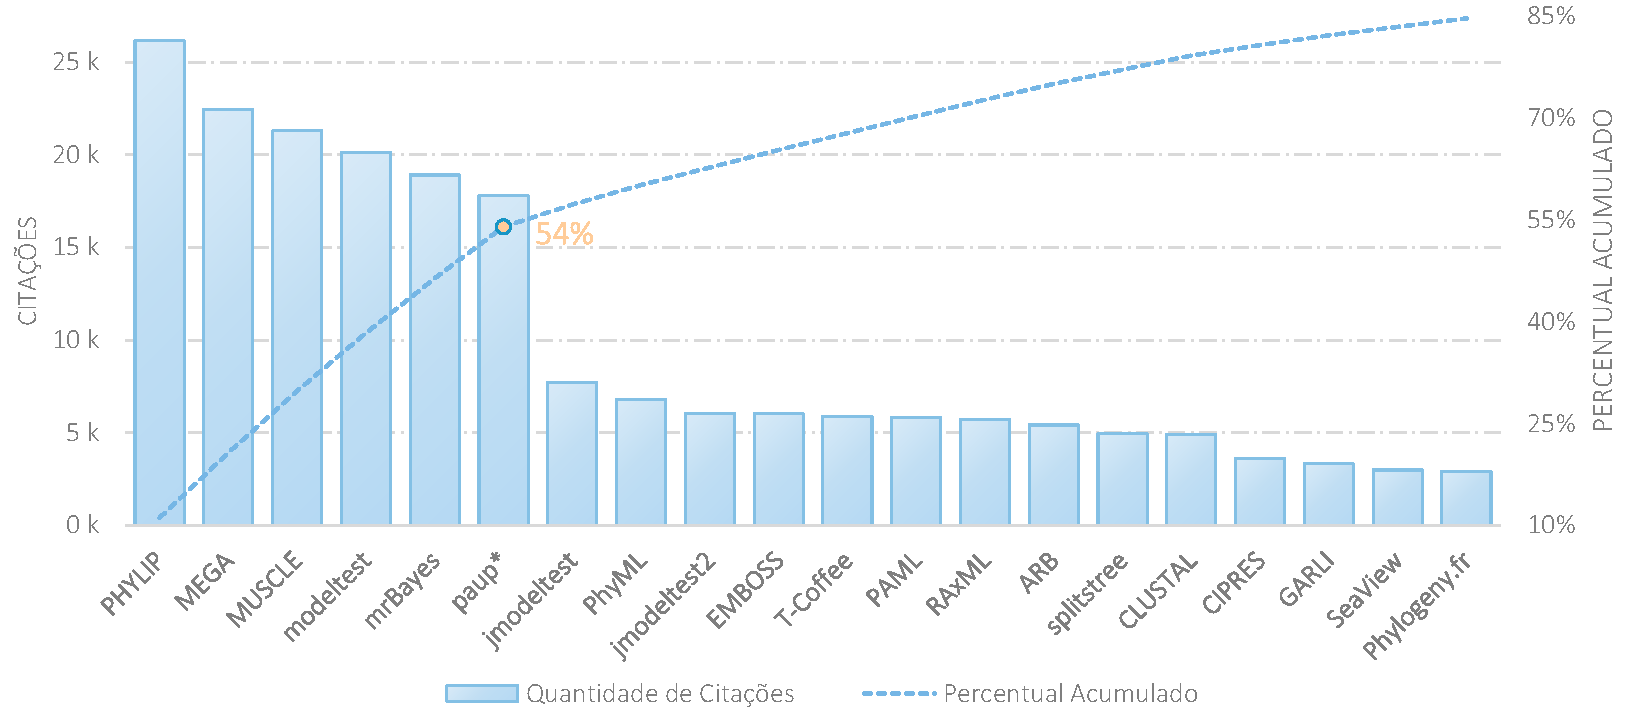
\includegraphics[width=\textwidth]{survey-topcitations}
		\fonte{Elaborado pelo autor.}
	\end{minipage}
\end{figure}


Uma vez identificado o estado da arte no que diz respeito à intersecção das áreas de computação de alto desempenho e bioinformática, mais precisamente filogenética, foi verificada a existência de lacunas, detalhadas na \autoref{sec:lacunas-de-pesquisa}, quanto à técnicas computacionais modernas, como por exemplo: aceleração por GPUs, balanceamento de carga e o uso de recursos de computação em nuvem.
Embora todas as lacunas encontradas sejam relevantes para o aumento da eficiência dos projetos de software, o modelo \textsf{He}--lastic estreita seu foco na questão da elasticidade de recursos computacionais.
Desta forma, o presente trabalho objetiva modernizar projetos relevantes para a bioinformática, assim como, realizar ganhos de eficiência e possíveis reduções de custos, através do desenvolvimento de um modelo que seja capaz de validar a hipótese de que a computação em nuvem, através da elasticidade, pode fornecer os ganhos de eficiência e redução de custos.


Para identificar um projeto candidato dentre os 83 encontrados no levantamento bibliográfico (vide \autoref{tab:survey-comparativo}), recorreu-se a uma característica presente nas publicações oriundas da filogenética: o uso difundido da citação das ferramentas utilizadas como referências nas publicações da área.
Embora esta não seja uma característica exclusiva das publicações da filogenética, observações empíricas pelo autor sugerem uma alta aderência a este padrão de comportamento.
Como consequência desta conduta torna-se possível identificar as ferramentas mais utilizadas e de maior impacto no dia a dia do pesquisador de bioinformática, viabilizando colocar em prática os objetivos previamente mencionados.


Desta forma, foi realizado o levantamento do número de citações para cada um dos 83 trabalhos encontrados através dos agregadores utilizados no levantamento bibliográfico (\autoref{tab:survey-sources}) como Google Scholar, CiteSeerX e SemanticScholar.
O resultado deste levantamento é apresentado na sua totalidade na \autoref{tab:survey-citecount}~(\autoref{sec:appendix-a}),
onde seis projetos se destacam dos demais em função de sua popularidade:
\begin{inparaenum}[\itshape a\upshape)] 
	\item PHYLIP 	-- \citetexto{Felsenstein1989};
	\item MEGA 		-- \citetexto{Kumar2016};
	\item MUSCLE 	-- \citetexto{Edgar2004};
	\item modeltest -- \citetexto{Posada1998};
	\item mrBayes 	-- \citetexto{Huelsenbeck2001}; e
	\item paup* 	-- \citetexto{Swofford2002}.
\end{inparaenum}
Dada a grande quantidade de trabalhos oriundos do levantamento bibliográfico, foi necessário recorrer a uma variação do princípio de Pareto\footnote{
	O princípio de Pareto, \cite{ParetoPrinciple}, é uma famosa afirmação de que 80\% dos efeitos vêm de 20\% das causas. Este princípio é muito observado em empresas como uma estratégia para priorizar os esforços de maneira a obter os maiores retornos.
} visando reduzir a lista para contemplar somente os trabalhos mais citados e que em conjunto acumulam 85\% das citações totais, descartando a cauda longa, ou seja, trabalhos de baixa relevância bibliográfica.


A aplicação desta estratégia resultou na seleção dos vinte primeiros trabalhos ordenados de acordo com o número de citações, e pode ser vista na \autoref{fig:survey-topcitations}.
Dentre esta lista de artigos chama a atenção a presença de três variantes de softwares utilizados para o cálculo de \textit{best--fit} de sistemas de substituição filogenética, o MODELTEST de \citetexto{Posada1998}, o jModelTest de \citetexto{Posada2008} e o jModelTest2 de \citetexto{Darriba2012}, que somados ultrapassariam o projeto PHYLIP, como mais citados neste levantamento.
Quando considerada a importância da correta seleção do sistema de substituição genética, conforme abordado na \autoref{sec:modelos-de-substituicao}, a quantidade de citações se mostra plausível e pode, até mesmo, comprovar quão difundida é a prática entre bioinformatas.


\begin{figure}[tb]
	\centering%
	\begin{minipage}{\defaultFigureWidth\textwidth}
		\caption{Linha do tempo do projeto jModelTest: histórico de publicações relevantes para compreensão do contexto, objetivos e evolução da ferramenta.}
		\label{fig:jmodeltest-history}
		\begin{NoHyper}
		\begin{chronology}[4]{1996}{2019}{\defaultFigureWidth\textwidth}
			\eventUP{1997}{Base Teórica --- \citetexto{Huelsenbeck1997}}
			\eventDOWN{1998}{MODELTEST --- \citetexto{Posada1998}}
			\eventUP{2003}{Guia de uso MODELTEST --- \citetexto{Posada2003a}}
			\eventDOWN{\decimaldate{01}{04}{2003}}{Capítulo de Livro --- \citetexto{Posada2003b}}
			\eventUP{2005}{ProtTest --- \citetexto{Abascal2005}}
			\eventDOWN{2008}{jModelTest --- \citetexto{Posada2008}}
			\eventUP{2010}{jModelTest em grid --- \citetexto{Loureiro2010}}
			\eventDOWN{\decimaldate{01}{04}{2010}}{ProtTest-HPC --- \citetexto{Darriba2010}}
			\eventUP{2011}{ProtTest 3 --- \citetexto{Darriba2011}}
			\eventDOWN{2012}{jModelTest2 --- \citetexto{Darriba2012}}
			\eventUP{2014}{jModelTest.org --- \citetexto{Santorum2014}}
		\end{chronology}
		\end{NoHyper}
		\fonte{Elaborado pelo autor.}
	\end{minipage}
\end{figure}


Como resultado desta análise o projeto jModelTest2 de \citetexto{Darriba2012} se apresenta como alvo e ponto de partida dos esforços de atualização e melhoria tecnológica no contexto da bioinformática e da inferência filogenética através do uso do modelo \textsf{He}--lastic.
Com o objetivo de destacar para o leitor as publicações que contribuem para o entendimento das motivações e histórico dos desenvolvimentos que compõem a ferramenta, são apresentadas a seguir as origens do jModelTest2 e a relação entre autores e projetos relacionados.
Desde o estabelecimento das fundações teóricas em 1997\footnote{
	\citetexto{Huelsenbeck1997}
} até um portal \textit{web} em 2014\footnote{
	\citetexto{Santorum2014}
}, é apresentada na \autoref{fig:jmodeltest-history} uma linha do tempo com os pilares que trouxeram o projeto até os dias de hoje, seja no quesito autores\footnote{
	Darriba parece ser o atual responsável pelo projeto, tendo herdado de Posada que o iniciou em colaboração com Crandall.
} (de Crandall para Posada e, por fim, Darriba) ou no que diz respeito a softwares\footnote{
	MODELTEST\textsuperscript{\dag} foi o precursor direto do jModelTest que, no princípio, trabalhava apenas com um conjunto restrito de sistemas de substituição nucleotídica, no entanto ao longo da história suas funcionalidades parecem ter se fundido com o ProtTest\textsuperscript{\dag} herdando a capacidade de avaliar sistemas de substituição proteica e aumentando a quantidade de sistemas disponíveis para teste de adequação.
} (começando no MODELTEST, evoluindo para jModelTest e unindo forças com ProtTest).
%
Daqui em diante o projeto como um todo poderá ser denominado apenas jModelTest, embora se refira especificamente à versão 2 do programa.


% delimita o bloco da footnote da footnote
{
	\renewcommand*{\thefootnote}{\fnsymbol{footnote}}
	\addtocounter{footnote}{0}\footnotetext[2]{
		Aparentemente descontinuados e/ou obsoletos.
	}
	\renewcommand*{\thefootnote}{\arabic{footnote}}
}


Programado na linguagem Java, o jModelTest2 contém uma interface gráfica acoplada ao programa e é facilmente executado em múltiplas plataformas através do \textit{runtime} Java.
O código fonte está disponível online, juntamente com o histórico de versionamento no portal \href{https://github.com/ddarriba/jmodeltest2}{Github}\footnote{
	Disponível na URL \url{https://github.com/ddarriba/jmodeltest2}.
}, facilitando a exploração do projeto e permitindo acompanhar sua evolução ao longo do tempo.
O projeto está acompanhado de múltiplos artigos que abordam seu funcionamento e embasamento teórico, vide \autoref{fig:jmodeltest-history},
porém seu uso é simples e direto, apesar de exigir conhecimentos avançados da área de atuação para a compreensão dos resultados, ou seja, o grau de adequação dos sistemas de substituição de sequências moleculares e seus parâmetros.



Conforme previamente abordado na \autoref{sec:analise-estadodaarte} e na \autoref{tab:survey-comparativo}, o jModelTest tem suporte explícito à múltiplas CPUs, seja localmente, ou até mesmo, em ambientes MPI.
Outra característica importante do programa é que a natureza do trabalho realizado permite um alto grau de paralelismo \cite{Keane2006a}, uma vez que o teste de cada um dos sistemas de substituição de sequências pode ser realizado de maneira independente dos demais.
Estas e outras características técnicas serão abordadas em maior profundidade nas próximas seções.


Embora haja menção ao uso de computação em nuvem, através de testes em instâncias 
EC2\footnote{
	Serviço que fornece máquinas virtuais disponibilizadas pelo provedor de computação em nuvem AWS.
} 
e documentado em \citetexto{Darriba2012}, o cenário explorado segue um modelo de recursos fixos e predefinidos, efetivamente simulando um \textit{cluster}, e, portanto, não se beneficiando da elasticidade de recursos disponível nestes ambientes.
Ainda assim, o programa consegue obter desempenho razoável ao fazer uso de todos os processadores disponíveis durante sua execução e se mostrar apto a trabalhar no ambiente de computação em nuvem sem a necessidade de significativas modificações em seu código ou procedimentos.



\begin{figure}[tb]
	\centering%
	\begin{minipage}{\defaultFigureWidth\textwidth}
		\caption[Exemplo minimalista do fluxo de tarefas típico para realização de análises filogenéticas no laboratório de filogenética da UNISINOS]{Exemplo minimalista do fluxo de tarefas típico para realização de análises filogenéticas no laboratório de filogenética da UNISINOS: Coleta de amostras através do banco de dados NCBI, Alinhamento de Sequências usando os projetos MEGA ou SeaView, Seleção de sistemas de substituição com a ajuda do jModelTest e, finalmente, Inferência filogenética por métodos Bayesianos com o projeto BEAST.}
		\label{fig:modelo-workflow-unisinos}
		\vspace{1ex}
		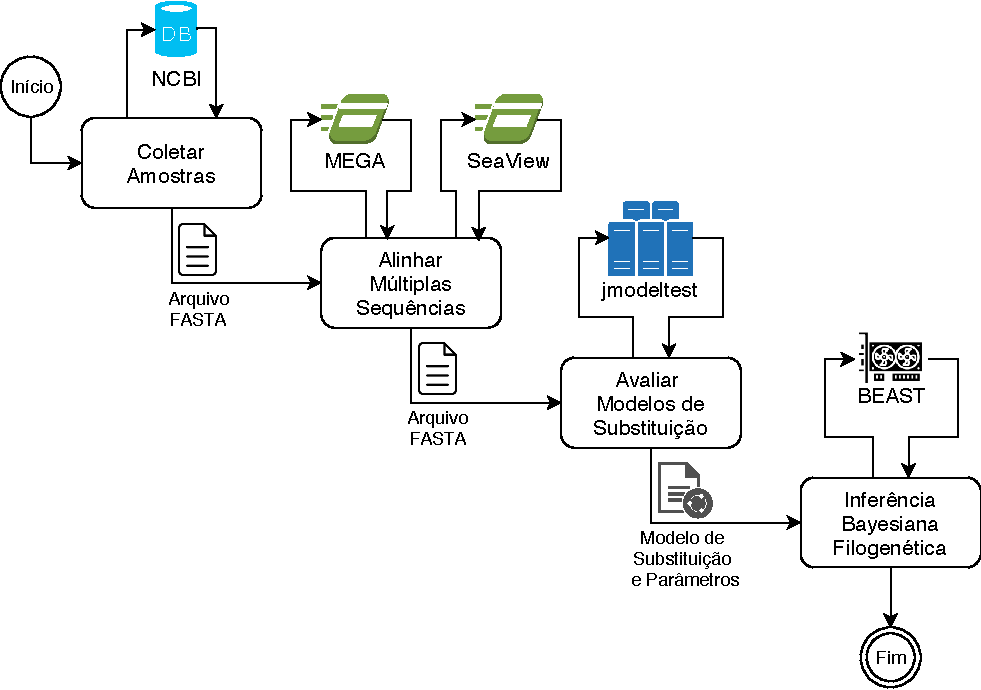
\includegraphics[width=\textwidth]{workflow-biologia}
		\fonte{Elaborado pelo autor com base em comunicação pessoal com membros da equipe de estudos filogenéticos da UNISINOS.}
	\end{minipage}
\end{figure}


Além da popularidade do projeto, evidenciada pelo número de citações, outro fator relevante para sua escolha está no fato de que, no processo de análise e inferência filogenética, a seleção de um sistema de substituição molecular é um dos passos preparatórios à análise propriamente dita, assim como a coleta de amostras e o alinhamento de sequências moleculares.
Contudo, apesar do seu carácter preparatório, este costuma ser um passo demorado em função do custo computacional da avaliação de \textit{best--fit}, dentre os inúmeros sistemas de substituição, assim como, de suas variantes, e também o conjunto de dados a ser analisado.


De acordo com levantamento realizado junto ao laboratório de filogenética da UNISINOS, em um típico fluxo de tarefas para análise filogenética (como aquele apresentado na \autoref{fig:modelo-workflow-unisinos}), a seleção de sistemas pode levar diversas horas e, conforme o tamanho e a quantidade dos alinhamentos de sequências, nem mesmo chega a terminar, esbarrando em limitações técnicas.
Esta lentidão no processo de busca do sistema mais adequado aos dados pode fazer com que pesquisadores negligenciem a importância de escolher o sistema correto, o que, segundo advertem \citetexto{Minin2003} e \citetexto{Keane2006a}, pode levar a conclusões infundadas e puramente erradas.


Sendo assim, uma possível redução no tempo de execução destes cálculos traz duplos benefícios ao: 
\begin{inparaenum}[\itshape a\upshape)] 
	\item incentivar aqueles que atualmente não efetuam uma rigorosa seleção de sistemas a fazê-lo; além de 
	\item conceder mais tempo livre para análises mais profundas aos pesquisadores que já utilizam o processo de seleção.
\end{inparaenum}
Podendo, em última instância, aumentar a qualidade da produção acadêmica em ambos os casos.


\section{Decisões de Projeto}
\label{sec:modelo-decisoes}


%Keane2006a
%The task of testing multiple substi-tution models against an alignment is very amenable to parallelisation as
%each model can be optimised completely independently and the correspond-ing likelihoods can be collected and analysed at the server to determine the
%optimal model. Clearly the simplest and most efficient way to parallelise ML
%model selection is to simply issue each model to a processor to be optimised.


Originalmente detalhado em \citetexto{Posada2008}, com melhorias no campo da computação de alto desempenho, delineadas posteriormente em \citetexto{Darriba2014}, a principal função do projeto jModelTest é encontrar o sistema de substituição molecular que melhor se encaixa ao alinhamento de sequências informado como entrada, em um processo chamado de \textit{best--fit}.
Esta tarefa é altamente receptiva ao paralelismo, uma vez que, cada sistema pode ser testado individualmente e os resultados coletados e comparados ao final do processo, elencando o sistema mais adequado, segundo algum critério de priorização ou ranqueamento \cite{Keane2006a}.


Contudo, apesar da aparente simplicidade da tarefa, um fator relevante no esforço computacional é a complexidade do sistema de substituição molecular.
Conforme abordado na \autoref{sec:modelos-de-substituicao}, nem todos os sistemas são criados iguais, com a complexidade aumentando progressivamente ao longo dos anos e acompanhando a profundidade do conhecimento acerca dos processos evolutivos.
Desta forma seria intuitivo pensar que devemos sempre usar o sistema mais complexo possível, uma vez que este será capaz de melhor se adaptar aos dados encontrados. 
No entanto, este não é o caso, pois como afirma \citetexto{Zwickl2006}, além de exigir maior esforço computacional, um sistema muito complexo está mais vulnerável ao risco de atribuir grande importância a algum tipo de ruído aleatório presente nos dados.


Para combater estes riscos é comum que critérios de seleção de sistemas, como os critérios de informação de Akaike \cite{Akaike1974} e Bayesianos \cite{Schwarz1978}, penalizem a complexidade dos sistemas durante a escolha do \textit{best--fit} \cite{yang2014molecular}.
Esta política implica na avaliação de todos os sistemas disponíveis, dos mais simples aos mais complexos, para obter um panorama da adequação aos dados, o que, computacionalmente, gera tarefas com grande variação na complexidade dos cálculos e consequente carga computacional.
Desta forma, ainda que paralelizável, o cálculo de adequação do sistema é uma tarefa com ampla variação no esforço necessário, o que, conforme pode ser observado na \autoref{fig:modelo-ociosidade}, desafia estratégias ingênuas de computação paralela e distribuída em função do desbalanceamento da carga computacional entre os nodos disponíveis.


\begin{figure}[tb]
	\centering%
	\begin{minipage}{\defaultFigureWidth\textwidth}
		\caption{Representação de carga em múltiplos processadores ou nodos durante a execução de processos com complexidade variável, exemplificando o cenário encontrado pela aplicação jModelTest durante o teste de adequação de sistemas de substituição de sequências moleculares onde parte significativa dos recursos pode permanecer ociosa enquanto aguarda a conclusão dos cálculos que exigem maior poder computacional.}
		\label{fig:modelo-ociosidade}
		\centering
		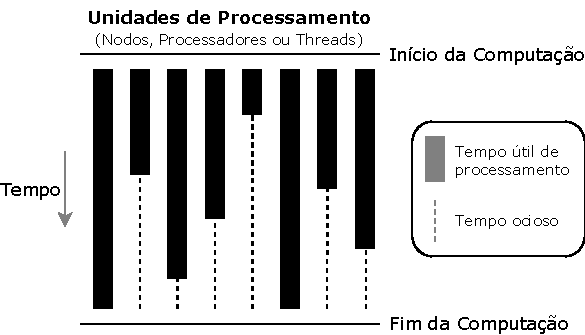
\includegraphics{modelo-ociosidade}
		\fonte{Elaborado pelo autor.}
	\end{minipage}
\end{figure}


Dependendo das configurações selecionadas pelo usuário para início da análise o número de sistemas simulados pode variar amplamente, com possibilidades tão baixas quanto apenas três sistemas, ou tão altas quanto 1624 variações dos sistemas de evolução para teste.
Quando executado em um computador de mesa, ou até mesmo, um servidor institucional, é possível que o hardware fique subutilizado, embora seja pouco provável, uma vez que as probabilidades estejam a favor de que este se torne um gargalo, haja vista que as configurações padrão geram 88 cenários de teste, enquanto um computador de mesa conta atualmente com um número entre 4 a 16 \textit{cores} de processamento.
Ainda, no que diz respeito aos fatores que influenciam a carga computacional durante o cálculo, quatro são especialmente importantes no contexto deste trabalho:


\begin{enumerate}[label={\arabic*)}]
	\phantomsection
	\label{list:fatores-influenciam-performance}
	
	\item Escolha dos sistemas elencados para o teste de adequação;
	
	\item Complexidade inerente a cada sistema\footnote{
		Geralmente medida em termos da quantidade de parâmetros livres sujeitos à otimização.
	};
	
	\item Quantidade de sequências moleculares; e
	
	\item Comprimento das sequências moleculares\footnote{
		Geralmente medido em termos do número de caracteres que compõem a sequência.
	};
\end{enumerate}


A partir destes quatro elementos é possível estabelecer uma série de equações que determinam o comportamento computacional de uma execução do processo de adequação de sistemas de evolução filogenética através do software jModelTest.
O cálculo do custo de uma execução do jModelTest é obtido através da \autoref{eq:custo-jmodel-bestfit} (detalhada na \autoref{tab:custo-jmodel-elementos}) que, de acordo com os fatores previamente citados, combina o custo oriundo dos dados do arquivo de alinhamentos com o custo obtido através das escolhas de parâmetros para a execução, ambos detalhados a seguir.
A \autoref{eq:custo-jmodel-arquivo} detalha o custo computacional oriundo do arquivo, $ C_a(i,c) $, usado como parâmetro de entrada para o programa jModelTest. 
Este arquivo deve conter um alinhamento de sequências moleculares compostas por amostras de uma determinada região de comprimento $ c $ de uma lista de indivíduos $ i $.


\begin{table}[tb]
	\centering%
	\begin{minipage}{\defaultFigureWidth\textwidth}
		\caption{Detalhamento das variáveis e funções utilizadas na definição de custo de execução do jModelTest.}
		\label{tab:custo-jmodel-elementos}
		\small
		\vspace{1ex}
		\renewcommand\arraystretch{1.4}
		\renewcommand {\tabularxcolumn}[1]{>{\arraybackslash}m{#1}}
		\begin{tabularx}{\textwidth}{cX@{}}
			\toprule
			Variável / Função & Descrição \\ 
			\midrule
			$ i $ & Quantidade de indivíduos / amostras contidos no arquivo de alinhamento de sequências moleculares \\
			$ c $ & Comprimento da região molecular de interesse (geralmente uma região do código genético ou um gene específico) \\
			$ s $ & Lista dos sistemas de modelagem do processo de evolução / substituição molecular (por exemplo os contidos na \autoref{tab:models}) \\
			$ C_a(i,c) $ & Custo oriundo do arquivo de alinhamento de sequências moleculares \\
			$ C_p(s) $ & Custo oriundo dos parâmetros escolhidos pelo usuário durante a execução do programa \\
			$ C_s $ & Custo de um sistema de substituição molecular \\
			$ C(i,c,s) $ & Custo total de uma execução do jModelTest \\
			\bottomrule	
		\end{tabularx}
		\fonte{Elaborado pelo autor.}
	\end{minipage}
\end{table}


\begin{equation}
\label{eq:custo-jmodel-arquivo}
% custo do arquivo = individuos X comprimento das sequências
C_a(i,c) = i \times c
\end{equation}
\begin{equation}
\label{eq:custo-jmodel-params}
% custo do parametros = soma das custos de cada sistema selecionado
C_p(s) = \sum_{k=1}^{n} C_s(s_k)
\end{equation}
\begin{equation}
\label{eq:custo-jmodel-bestfit}
C(i,c,s) = C_a(i,c) \times C_p(s)
\end{equation}


A seguir, na \autoref{eq:custo-jmodel-params}, é demonstrado o cálculo do custo computacional em função dos parâmetros de execução, $ C_p(s) $, sendo o principal elemento a variável $ s $ que representa uma lista de sistemas de substituição de sequências moleculares, onde o resultado desta equação é a soma dos custos de cada um dos sistemas escolhidos. 
Esta lista contém cada um dos sistemas de sustituição a ser testados pelo software em busca daquele que melhor representa os dados, no processo de \textit{best--fit}, e é obtida através da combinação dos parâmetros informados pelo usuário durante o uso do software.
Embora o custo computacional do cálculo de cada sistema não seja abordado neste trabalho, ele é explorado em profundidade nas teses de \citetexto{Keane2006a}, \citetexto{Zwickl2006} e \citetexto{DarribaPHD}.


A proposta descrita neste capítulo adotou decisões diretamente influenciadas pelo contexto apresentado na \autoref{sec:modelo-decisoes}, assim como, os requisitos definidos pelos objetivos deste trabalho (detalhados na \autoref{sec:objetivos}) e as lacunas de pesquisa encontradas durante a análise comparativa (\autoref{sec:lacunas-de-pesquisa}) dos trabalhos relacionados focando, todavia, na questão da elasticidade no consumo de recursos computacionais.
Tais decisões formam as premissas básicas que fundamentam a arquitetura do modelo proposto, atuar como guias sobre qualquer desenvolvimento realizado.
Com este cenário em mente foram estabelecidas as seguintes decisões de projeto:
\begin{enumerate}[label=Decisão~\arabic*:,itemindent=*,leftmargin=*]
	\phantomsection
	\label{list:decisoes-de-projeto}
	
	\item Deve tirar proveito das funcionalidades disponíveis em um ambiente de computação em nuvem;

	\item Deve suportar a elasticidade de recursos computacionais a nível de seus algoritmos\footnote{
	Descartando, desta forma, estratégias de elasticidade baseadas na quantidade de usuários paralelos do sistema, como no modelo clássico de elasticidade para aplicações web e \textit{e--commerce} com um balanceador de carga distribuindo requisições para um conjunto de réplicas de máquinas virtuais.
};
	
	\item Deve lidar com a variabilidade na carga computacional oriunda das características do teste de adequação de sistemas de substituição molecular;
	
	\item Deve permanecer agnóstico a provedores de computação em nuvem, evitando depender de funcionalidades exclusivas da plataforma;
	
	\item Deve manter a configuração tão simples quanto possível, idealmente limitando-se às regras de elasticidade;

	\item Deve empenhar-se em reduzir a carga operacional, delegando tarefas de gestão para o provedor de computação em nuvem; e

	\item Deve buscar uma melhor relação custo-benefício em comparação às soluções existentes.
\end{enumerate}


\section{Arquitetura}
\label{sec:modelo-arquitetura}


\begin{figure}[tb]
	\centering%
	\begin{minipage}{\defaultFigureWidth\textwidth}
		\caption{Visão conceitual do modelo \textsf{He}--lastic ilustrando como suas duas camadas de elasticidade interagem para atender requisições.}
		\label{fig:modelo-conceitual}
		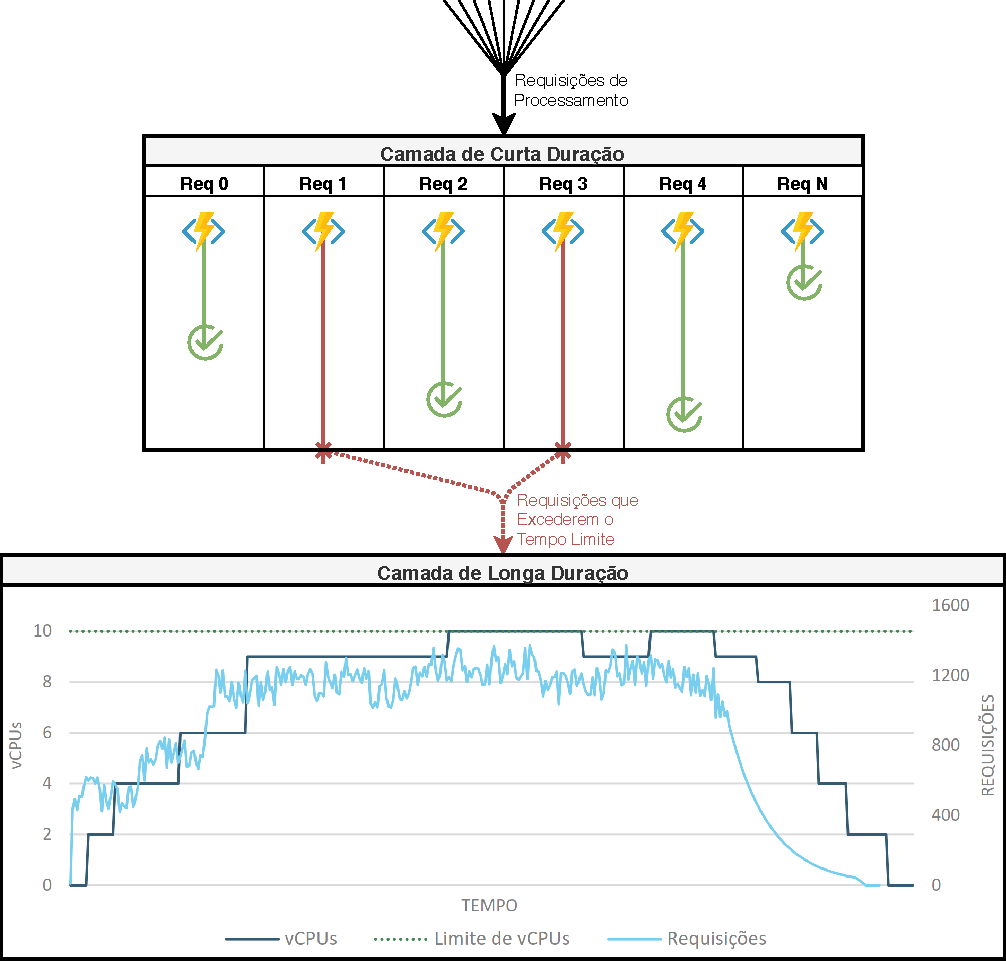
\includegraphics[width=\textwidth]{modelo-conceitual}
		\fonte{Elaborado pelo autor.}
	\end{minipage}
\end{figure}


\begin{table}[tb]
\centering%
\begin{minipage}{\defaultFigureWidth\textwidth}
	\caption{Parâmetros necessários para a configuração do modelo \textsf{He}--lastic.}
	\label{tab:modelo-arq-params}
	\small
	\vspace{1ex}
	\renewcommand\arraystretch{1.4}
	\renewcommand {\tabularxcolumn}[1]{>{\arraybackslash}m{#1}}
	\begin{tabularx}{\textwidth}{lp{7em}X@{}}
		\toprule
		Camada & Parâmetro & Descrição \\ 
		\midrule
		\multirow{2}{*}[-2em]{\begin{tabular}[c]{@{}c@{}}Curta~Duração\\ FaaS\end{tabular}} & Tempo Limite & Tempo máximo de processamento para os processos executando nesta camada. \\
		& Potência & Determina o poder de processamento alocado para cada unidade de execução na camada. Geralmente se manifesta como uma medida de memória alocada, embora possa ser composta por outras métricas (vide \autoref{tab:FaaS-implementations}). \\
		%\cmidrule{2-3}
		\dashedline{2-3}
		\multirow{3}{*}[-3em]{\begin{tabular}[c]{@{}c@{}}Longa~Duração \\ Orquestrador\\ de Contêineres\end{tabular}} & Número de CPUs & Quantidade limite de CPUs disponíveis para uso. Tem por objetivo garantir a previsibilidade de custos para esta camada. \\
		& Limite Inferior de Carga & \textit{Threshold} indicativo da ocupação mínima permitida para cada VM da camada. A violação deste limite causará uma ação de elasticidade para consolidação / redução de recursos. \\
		& Limite Superior de Carga & \textit{Threshold} indicativo da ocupação máxima permitida para cada VM da camada. A violação deste limite causará uma ação de elasticidade para replicação / incremento na quantidade de recursos. \\
		\bottomrule	
	\end{tabularx}
	\fonte{Elaborado pelo autor.}
\end{minipage}
\end{table}


O modelo elaborado, batizado de \textsf{He}--lastic, busca, através da elasticidade de recursos computacionais, balancear performance computacional, medida pelo tempo de execução, com custo financeiro através do uso consciente de recursos, ao lançar mão da funcionalidade mais adequada para cada tipo de processo em execução.
Tal estratégia é factível em função da divisão em camadas de elasticidade proposta pelo modelo (ilustrada na \autoref{fig:modelo-conceitual}), onde cada uma apresenta características complementares e melhor adaptadas para classes distintas de processos.
Portanto, é na divisão em camadas de elasticidade, abordada em detalhes na \autoref{sec:estrategias-elasticidade}, que encontra-se o ponto fundamental de diferenciação do modelo \textsf{He}--lastic. 



Do ponto de vista do usuário da aplicação jModelTest as mudanças são mínimas, uma vez que sua execução se dá por interface gráfica ou linha de comando e o efetivo processamento já ocorre em plano de fundo, assim como é previsto com a adoção do modelo proposto.
Desta forma, cabe salientar que o jModelTest oferece uma interface gráfica para uso interativo além do uso por linha de comando, embora este último seja recomendado para usuários experientes, dado que é mais confiável e apropriado para integração com demais etapas do \textit{pipeline} de análise filogenética.
No que diz respeito ao processamento, referente ao cálculo de \textit{best--fit} de sistemas de substituição de sequências moleculares, que executa em \textit{background}, o jModelTest oferece opções via memória compartilhada, com o uso de múltiplas \textit{threads} de processamento, e através da biblioteca paralela MPI, recomendada para ambientes de \textit{cluster}.
Uma vez que os cálculos de \textit{best--fit}, que compõem a parte mais relevante do custo computacional, já são executados em \textit{background}, não é esperado impacto no uso da ferramenta por parte do usuário final em função da adoção do modelo \textsf{He}--lastic, podendo ser visto como a implementação de um \textit{back--end} SaaS para o jModelTest, uma vez que isola do usuário todo o trabalho de configuração e pode ser acessado como uma API.



Ainda assim, existe a necessidade de configurar alguns parâmetros de execução referentes ao ambiente de computação em nuvem e fundamentais para o bom funcionamento do modelo, conforme detalhados na \autoref{tab:modelo-arq-params}.
Neste caso, a figura de um administrador de ambientes deve ser prevista.
Embora este perfil de usuário não seja mencionado nas publicações e documentações do projeto jModelTest, é natural projetar a sua existência para qualquer cenário de uso exceto os mais simples.
Tal afirmação deve-se à necessidade de separar o usuário com conhecimentos em bioinformática (exerce domínio sobre conhecimentos da biologia e suas ferramentas, contudo é incapaz de executar tarefas computacionais mais avançadas) do administrador, um perfil com profundo conhecimento computacional, capaz de provisionar servidores, configurar ambientes e montar \textit{clusters} computacionais.
%
Cabe, também, ao administrador determinar os valores para os parâmetros de operação do modelo, uma tarefa que pode ser realizada de maneira empírica através de experiência ou observações, ou seguindo uma abordagem mais científica através de uma análise de cenários de custo--benefício, como será detalhado na \autoref{sec:modelo-custben}.



As tarefas de responsabilidade do administrador tornam-se necessárias a partir do momento em que os recursos locais do usuário bioinformata deixam de ser suficientes para suas análises, sendo este o mesmo momento em que ele potencialmente buscará por alternativas como o modelo \textsf{He}--lastic aqui proposto, o que leva à conclusão de que, mesmo com alguma parametrização necessária no ambiente de nuvem, este não é um fator de diferenciação entre o \textsf{He}--lastic e o jModelTest, principalmente em cenários em que há o uso de \textit{clusters} MPI.
Ademais, o reduzido número de parâmetros exigidos pelo \textsf{He}--lastic limita a profundidade do conhecimento necessário, sendo este um benefício oriundo da utilização da computação em nuvem.


Embora as camadas de elasticidade componham o cerne do modelo \textsf{He}--lastic, os demais componentes devem ser abordados para uma visão holística da proposta antes que se possa focar em seus detalhes, conforme abordado na \autoref{sec:estrategias-elasticidade}, onde são exploradas as características das camadas de elasticidade e seus parâmetros, assim como sua influencia sobre seu funcionamento.
A seguir, é fornecida uma descrição a respeito de todos os elementos presentes na arquitetura do modelo \textsf{He}--lastic, elucidando suas funções, interações e principais características, sendo esta dividida em dois grandes contextos, o do ambiente local e o de computação em nuvem.
Tal divisão se origina a partir do cenário de uso do \textit{software} jModelTest, baseado em interface gráfica, onde um pesquisador de bioinformática deseja executar seu teste de adequação de sistemas de substituição molecular a partir de sua estação de trabalho, enquanto tira proveito do poder computacional fornecido através da computação em nuvem.
Visando atender este cenário a arquitetura do modelo \textsf{He}--lastic requer os seguintes componentes:

\begin{itemize}
	
	\item \textbf{Ambiente local:} 
	neste contexto se concentram os componentes que interagem direta ou indiretamente com o usuário final da aplicação, sendo o programa jModelTest o principal deles.
	Para atingir o objetivo de incrementar as funcionalidades do mesmo, enquanto possibilita o aproveitamento de recursos da computação em nuvem, é necessária a introdução de um componente denominado \textquoteleft Módulo Mediador\textquoteright, que intermediará as ações computacionais assim como a comunicação com o programa jModelTest, passando a impressão de que, do ponto de vista do usuário, nada mudou.
	Este componente mediador é, por sua vez, composto por três subsistemas: 
	\begin{itemize}
		
		\item \textbf{Produtor:} traduz e transmite as solicitações de processamento geradas pela aplicação jModelTest para o ambiente de computação em nuvem, desencadeando o processamento destas;
		
		\item \textbf{Consumidor:} coleta os resultados das execuções que ocorreram no ambiente de computação em nuvem, reportando-os de volta em um formato compreendido pelo jModelTest;
		
		\item \textbf{Guardião\footnote{
	Durante testes locais com o jModelTest foram encontradas situações de exceção que levaram ao surgimento de processos órfãos, que continuavam consumindo recursos mesmo após o cancelamento da execução. Em um contexto de computação em nuvem uma situação como essa é particularmente perturbadora, pois pode acarretar em custos financeiros indesejados, justificando a necessidade de um subsistema dedicado.
}:}
		monitora e gerencia possíveis situações excepcionais observadas durante o processamento das requisições, tratando erros, se possível, e reportando tais situações ao programa jModelTest, enquanto aborta os demais processamentos em andamento, visando evitar desperdício de recursos.
		
	\end{itemize}

	
	\item \textbf{Ambiente de Computação em Nuvem:} 
	agrupados neste contexto estão os componentes responsáveis pela execução dos cálculos de adequação dos sistemas de substituição molecular, podendo ser denominado como o \textit{back--end} do modelo \textsf{He}--lastic por conter apenas componentes invisíveis do ponto de vista do usuário.
	Através do desacoplamento entre componentes é possível se manter fiel às decisões de projeto definidas na \autoref{sec:modelo-decisoes}, dando origem a uma arquitetura escalável e elástica enquanto suporta uma variada gama de provedores de computação em nuvem com reduzido fardo operacional para os administradores.
	São de fundamental importância neste ambiente os seguintes elementos:
	
	\begin{itemize}
		
		\item \textbf{Filas de Mensagens:}
%podem variar consideravelmente ao longo do tempo
%capacidade do sistema absorver picos de demanda
%e pode, também, servir como um dos sinais considerados em operações de elasticidade. Através
%de indicadores como tamanho da fila, taxa de entrada e de saída de mensagens é possível
%verificar a capacidade de processamento do sistema como um todo e, caso necessário, disparar
%ações de elasticidade. Tal estratégia é utilizada por Marshall, Keahey e Freeman (2010)
%O uso de filas e o processamento assíncrono também é uma recomendação
%tanto dos provedores de computação em nuvem quanto de acadêmicos, onde Tran, Skhiri e
%Zimányi (2011), por exemplo, afirmam que arquiteturas orientadas a eventos
%são um padrão de
%projeto recomendado para o paradigma de computação em nuvem e favorecem a elasticidade e
%a tolerância a falhas
por meio do uso de filas buscamos fornecer ao sistema os meios para se adaptar às variações de demanda e mantê-lo resiliente a falhas, uma vez que, processos com erros podem voltar para a fila ou ser direcionados para outro destino. Em se tratando de arquiteturas que visam elasticidade, tanto provedores de computação em nuvem, quanto acadêmicos como \citetexto{Tran2011}, recomendam o uso de filas e comunicação assíncrona orientada a eventos como padrão de projetos.
Seu uso é difundido entre iniciativas \textit{cloud--native} e suportado pelos principais provedores de computação em nuvem através de serviços gerenciados além de grande quantidade de alternativas \textit{open--source};
		
		\item \textbf{FaaS:}
utilizando recursos de FaaS podemos reduzir a carga administrativa, uma vez que fornecemos apenas o código para execução e podemos tirar proveito de uma frota virtualmente infinita de processadores.
Instâncias de funções são provisionadas sob demanda em segundos, escaladas elasticamente conforme a necessidade, com seu custo calculado por invocação e pelo produto do tempo de execução, de acordo com a quantidade de recursos utilizados, chegando a uma implementação quase perfeita do conceito \textit{pay-as-you-go} \cite{Spillner}, evitando ainda, custos com recursos inativos, pois os servidores permanecem sob gestão do provedor de computação em nuvem que é capaz de multiplexar seu uso entre clientes. 
Contudo, uma importante restrição das arquiteturas baseadas em FaaS é o limite no tempo de execução dos códigos e recursos computacionais relativamente restritos, o que torna esta modalidade inadequada para uma variedade de cenários;

		\item \textbf{Orquestrador de Contêineres:}
surge como um antídoto ao limite de tempo de execução dos FaaS ao fornecer, através da conteinerização, um ambiente similar ao de um FaaS, capaz de executar os mesmos códigos.
Contudo este não contam com a limitação relativa ao tempo de execução em troca de um maior fardo operacional, servindo, no modelo proposto, como um amortecedor, capaz de lidar com cálculos de longa duração e que seriam rejeitados pela camada de FaaS. 
Outro benefício é a redução na ocorrência de \textit{thrashing} de recursos computacionais, uma vez que temos a garantia (pela forma como a arquitetura do modelo está estruturada) de que todas as requisições encaminhadas para o orquestrador são de média a longa duração.
		
	\end{itemize}
	
\end{itemize}


\begin{figure}[tb]
\centering%
\begin{minipage}{\textwidth}
	\caption[Diagrama conceitual de alto nível da arquitetura do modelo \textsf{He}--lastic elucidando a relação entre seus componentes, assim como, a divisão em ambiente local e de computação em nuvem, com destaque para os elementos FaaS e Orquestrador de Contêineres, que representam as unidades de elasticidade do modelo, assim como as Filas de Mensagens que coordenam a comunicação entre os componentes do modelo]{Diagrama conceitual de alto nível da arquitetura do modelo \textsf{He}--lastic elucidando a relação entre seus componentes assim como, a divisão em ambiente local (responsável pela interação com o usuário) e de computação em nuvem (responsável pelos cálculos), com destaque para os elementos FaaS e Orquestrador de Contêineres, que representam as unidades de elasticidade do modelo, assim como as Filas de Mensagens que coordenam a comunicação entre os componentes do modelo}
	\label{fig:modelo-arq-full}
	\vspace{1ex}
	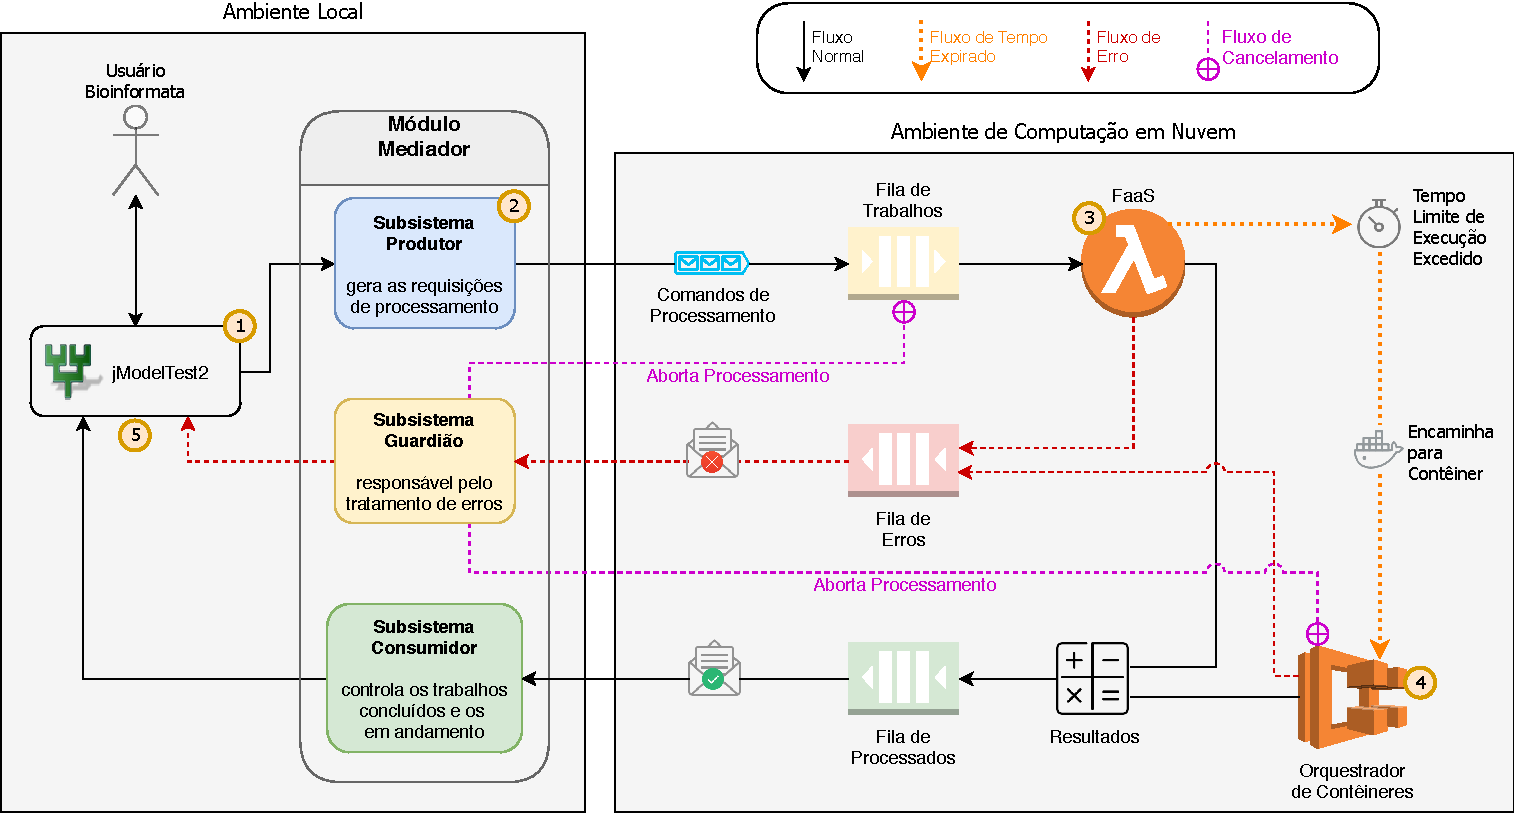
\includegraphics[width=\textwidth]{modelo-full}
	\fonte{Elaborado pelo autor.}
	%=======================================================================
	%		EXPLICAMENTO
	%=======================================================================
	%	\centering
	%	\begin{minipage}{.8\textwidth}
	%		\centering
	%		\vspace{1ex}
	%		\small
	%		\textbf{Fluxo de Execução:}
	%		\begin{enumerate}[leftmargin=*]
	%			\item Usuário interage com o jModelTest e dispara um teste de adequação de modelos de substituição;
	%			\item Módulo produtor da aplicação mediadora recebe o comando e cria uma série de tarefas e as submete através da fila de mensagens;
	%			\item O FaaS, primeira camada de elasticidade, recebe as tarefas e inicia o processamento utilizando o maior número possível de recursos disponibilizados pelo provedor de computação em nuvem;
	%			\item Aquelas tarefas que excedem o tempo limite de execução são encaminhadas para o Orquestrador de Contêineres, a segunda camada de elasticidade;
	%			\item Os resultados são devolvidos ao jModelTest através da aplicação mediadora onde, caso aconteça qualquer erro este causará o abandono da execução atual e cancelamento das demais tarefas.
	%		\end{enumerate}
	%	\end{minipage}
\end{minipage}
\end{figure}


\afterpage{%
	%\clearpage	% Flush earlier floats
	\begin{figure}[p]
		\vspace{-15.8ex}
		\hspace{-10.1ex}
		\begin{minipage}{1.16\textwidth}
			\caption{Diagrama UML de atividades do modelo \textsf{He}--lastic representando a interação, agrupada por etapa do processamento, entre os componentes da arquitetura.}
			\label{fig:modelo-uml-activity}
			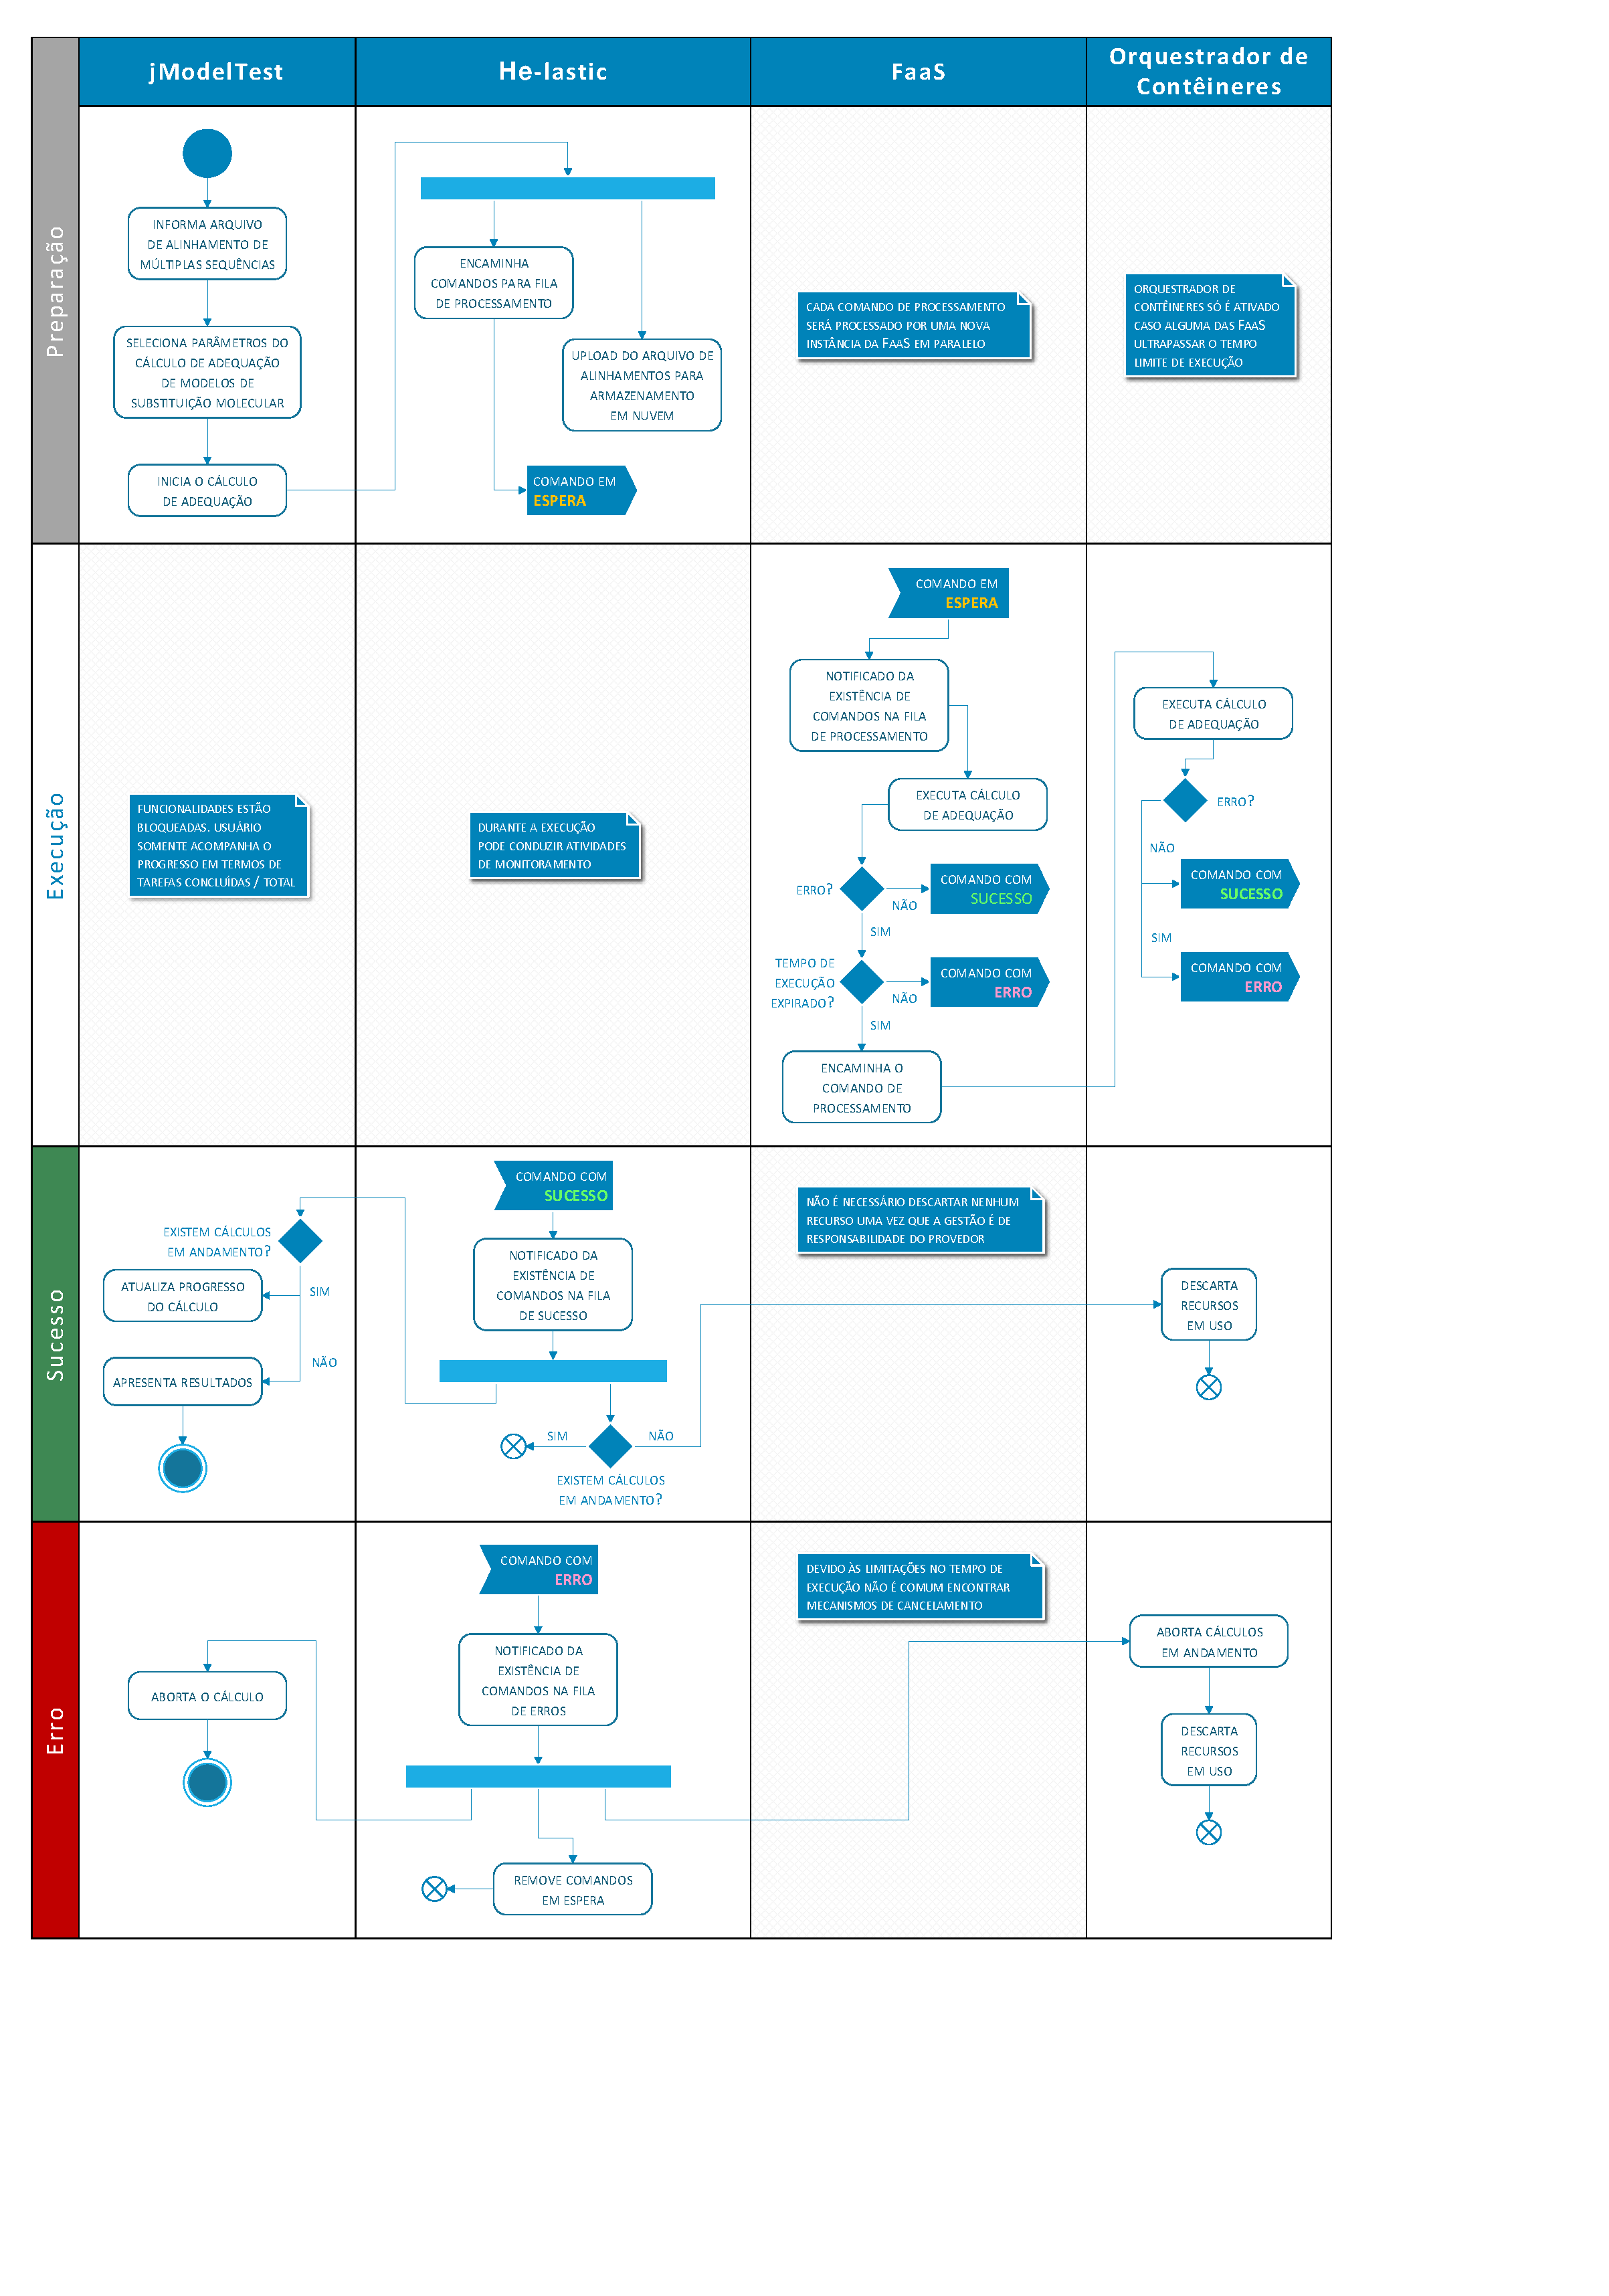
\includegraphics[trim=20 255 195 15,clip,width=\textwidth]{modelo-uml-activity}
			\fonte{Elaborado pelo autor.}
		\end{minipage}
	\end{figure}
}
\relax



Encontram-se representados na \autoref{fig:modelo-arq-full} os principais elementos do modelo, assim como, o relacionamento entre eles, com destaque para os dois grandes blocos que dividem o modelo em ambiente local e de computação em nuvem, sendo o primeiro responsável pela interação com o usuário, enquanto o segundo, tem como principal tarefa a execução dos cálculos para adequação do sistema de substituição molecular.
Estão destacados na figura cinco momentos distintos durante a execução do modelo \textsf{He}--lastic em conjunto com o jModelTest, sendo eles: 
%\begin{inparaenum}[\itshape 1\upshape)] 
\begin{enumerate}[label={\arabic*)}]

	\item o usuário bioinformata interage com o \textit{software} jModelTest, através de seu ambiente local, gerando requisições de processamento que serão interceptadas pelo Módulo Mediador do modelo \textsf{He}--lastic;

	\item de posse das requisições, o Subsistema Produtor traduz os comandos recebidos pelo jModelTest em requisições de processamento adequadas para o ambiente de computação em nuvem do modelo \textsf{He}--lastic e deposita estas mensagens em uma fila que alimenta a primeira camada de elasticidade;
	
	\item cada mensagem recebida pela Fila de Trabalhos causa a ativação de uma função FaaS correspondente tirando proveito das características dessa camada, principalmente, a capacidade de absorver picos repentinos de processamento, lançando mão do paralelismo massivo habilitado por uma frota de recursos ociosos gerenciados pelo provedor de computação em nuvem;
	
	\item contudo, é possível que determinadas requisições não possam ser atendidas na camada FaaS devido ao tempo limite de execução, cenário onde tais requisições serão encaminhadas para a segunda camada de elasticidade (vide \autoref{fig:modelo-conceitual}), o Orquestrador de Contêineres que representa um ambiente mais propício para execuções de longa duração e que demandam grande poder de processamento contínuo;
	
	\item ao fim do processamento, todos os resultados estarão disponíveis na Fila de Processados, que é monitorada pelo Subsistema Consumidor, responsável por encaminhar os resultados de volta ao \textit{software} jModelTest, com o Subsistema Guardião executando função análoga com relação aos possíveis erros ocorridos durante o processo.
\end{enumerate}
%\end{inparaenum}.



Uma vez detalhados os objetivos e os componentes do modelo torna-se possível a utilização de técnicas de projeto e arquitetura de \textit{software} para fornecer uma visão de alto nível e descrever as interações entre os elementos que compõem o modelo \textsf{He}--lastic.
Por meio da Linguagem Unificada de Modelagem (UML, no inglês), podemos representar formalmente o fluxo de controle entre os componentes do modelo, ou seja, seu comportamento, em um diagrama de atividades.
%
Este diagrama apresenta, conforme detalhado pela \autoref{fig:modelo-uml-activity}, no eixo vertical as etapas de execução do jModelTest, sendo compostas por { Preparação,  Execução, Erro e Sucesso} enquanto no eixo horizontal são descritos os princpais componentes do modelo.
%
Desta forma é possível identificar, por exemplo, a transição da camada FaaS para a camada de Orquestração de Contêineres através da leitura diagonal da esquerda para a direita e de cima para baixo, seguindo também as setas e seus possíveis locais de encaixe, que são representados pelo símbolo de evento, conforme a especificação UML
%
Os pontos de comunicação assíncrona através de filas de mensagens realizam a mediação entre ambiente local e de computação em nuvem além de favorecer o comportamento elástico através do desacoplamento, permitindo que cada componente do modelo atinja escalabilidade independentemente dos demais.





\section{Estratégias para Elasticidade}
\label{sec:estrategias-elasticidade}


\begin{table}[tb]
\centering%
\begin{minipage}{\defaultFigureWidth\textwidth}
	\caption[Comparativo entre as principais características das unidades de elasticidade utilizadas no modelo \textsf{He}--lastic]{Comparativo entre as principais características das unidades de elasticidade utilizadas no modelo \textsf{He}--lastic (maiores informações a respeito das implementações de FaaS podem ser encontradas na \autoref{tab:FaaS-implementations})}
	\label{tab:modelo-elasticidade-comparacao}
	\small
	\vspace{1ex}
	\renewcommand\arraystretch{1.4}
	\renewcommand {\tabularxcolumn}[1]{>{\arraybackslash}m{#1}} % vertical center
	\begin{tabularx}{\textwidth}{@{}rXX}
		\toprule
		& Orquestrador de Contêineres & FaaS \\ 
		\midrule
		Elasticidade & Através de mecanismos \newline Regra~---~Condição~---~Ação \newline (automática reativa) & Virtualmente infinita, uma nova instância para cada requisição \newline (orientada a eventos) \\
		Requisitos & Imagem do Ambiente \newline de Execução & Pacote com Código Fonte \\
		Carga Operacional & Maior & Menor \\
		Provisionamento & Em torno de Minutos & Em torno de Segundos \\
		Tempo de Execução & Ilimitado & Limitado em poucos Minutos \\
		Precificação & Por Hora & Por Segundo \\
		Ociosidade & Incorre Custos & Não Incorre Custos \\
		Adequação & Processos Longos & Processos Curtos \\ 
		\bottomrule
	\end{tabularx}
	\fonte{Elaborado pelo autor.}
\end{minipage}
\end{table}


\begin{figure}[tb]
\centering%
\begin{minipage}{\defaultFigureWidth\textwidth}
	\caption{Diagrama ilustrando as principais diferenças entre os componentes das camadas de elasticidade: Apesar de compartilharem a estrutura de alto nível, o FaaS tem importantes limitações no que diz respeito ao tempo de execução e capacidade de processamento, o que permite ao provedor de computação em nuvem otimizar a gestão da elasticidade e multiplexar o uso de recursos entre usuários; em contrapartida, o orquestrador de contêineres permite que o usuário determine o comportamento da elasticidade e abdica da limitação no tempo de execução em troca de um maior fardo operacional e um ambiente de execução que deve ser gerido pelo próprio usuário.}
	\label{fig:modelo-componentes-explodidos}
	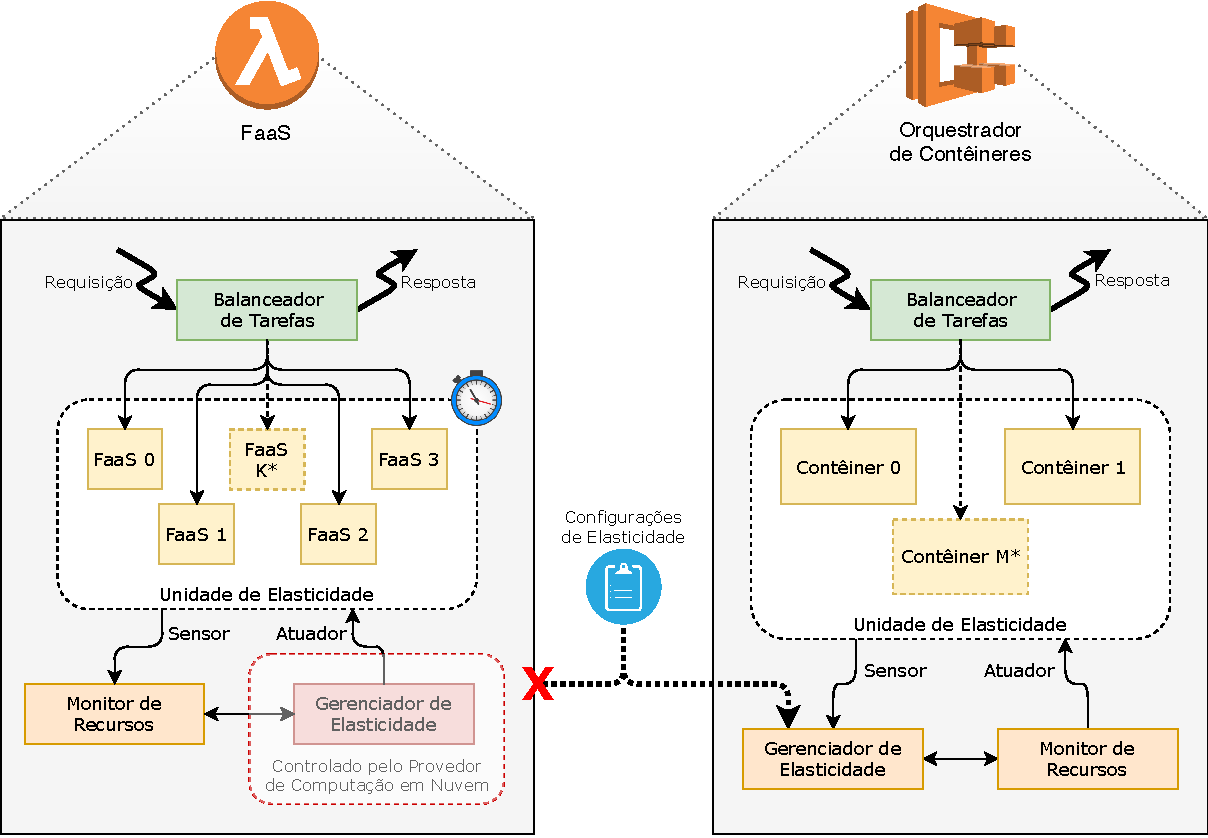
\includegraphics[width=\textwidth]{modelo-componentes-explodidos}
	\fonte{Elaborado pelo autor.}
\end{minipage}
\end{figure}







A interação entre os componentes previamente citados representa o cerne do modelo \textsf{He}--lastic que, através das suas duas unidades de elasticidade, nomeadamente o componente FaaS e o Orquestrador de Contêineres, operando na modalidade horizontal, com política automática reativa e estratégia por replicação (vide \autoref{sec:elasticidade}), possibilita um melhor acompanhamento da demanda computacional e economia ao evitar custos ociosos.
Estas duas unidades apresentam características distintas uma da outra, mas que se mostram, de certa forma, complementares.
Na \autoref{tab:modelo-elasticidade-comparacao}, uma comparação entre estas características é apresentada e, a seguir, uma descrição detalhada das mesmas.


Tarefas de média e longa duração são gerenciadas pelo Orquestrador de Contêineres que segue um modelo clássico de elasticidade automática reativa por replicação, distribuindo seu processamento entre uma frota de máquinas virtuais, que tem sua comunicação mediada por um balanceador de carga (embutido no orquestrador de contêineres).
Apesar da inexistência de restrições técnicas para o processamento de tarefas de curta duração, o modelo de precificação baseado em horas de uso, assim como, os \textit{delays} de início e término das máquinas virtuais (que contribui para o fenômeno conhecido como \textit{thrashing} \cite{Bersani2014}), faz com que tarefas curtas mereçam tratamento diferenciado, incrementando a complexidade de desenvolvimento e de operação.


Por este motivo o FaaS é empregado como uma solução para tarefas de curta duração, relevantes para o contexto da aplicação jModelTest, ao apresentar um modelo de precificação baseado em segundos de uso e empregar uma frota de máquinas virtuais gerenciadas e otimizadas pelos provedores de computação em nuvem, conforme abordado pela \autoref{fig:faas}.
Neste componente, os únicos requisitos são a definição da quantidade de recursos necessários e um pacote com o código fonte a ser executado por um dos ambientes oferecidos pelo provedor.


Do ponto de vista do programador, cada execução da sua função é análoga a iniciar uma instância, executar seu código e descartá-la.
Contudo, a gestão fica por conta do provedor, que é responsável pelo isolamento do ambiente e reaproveitamento de máquinas virtuais em execução.
Do ponto de vista da elasticidade, o uso de FaaS dá, ainda mais do que com a elasticidade clássica, a impressão de recursos ilimitados, uma vez que, para cada novo evento, um novo executor é alocado, possibilitando lidar facilmente com cargas de trabalho que ocorrem em rajadas (\textit{bursty workloads}).
Entretanto, este comportamento só é possível devido aos limites estabelecidos no tempo de execução de cada chamada, geralmente menores que 10 minutos, o que aumenta a rotatividade dos recursos e permite que o provedor de computação em nuvem absorva picos de demanda com capacidade ociosa através da multiplexação entre usuários.



Ao mencionar o modelo de elasticidade clássico, o presente trabalho faz referência a já amplamente estudada estratégia de elasticidade automática por replicação baseada em \textit{thresholds} superiores e inferiores que controlam a adição e remoção de máquinas virtuais dentre um \textit{pool} de recursos que fica acessível através de um balanceador de carga, como representado pela \autoref{fig:modelo-lb}~(\autoref{sec:appendix-a}).
Este modelo é muito popular entre aplicações comerciais como \textit{e--commerces}, portais e \textit{blogs}.
Todavia, seu uso no mundo acadêmico se mostra limitado quando confrontado com modelos de paralelismo como Fases Paralelas e Pipelines, conforme abordado em \citetexto{Aubin2015}, \citetexto{Aubin2016} e \citetexto{Aubin2017}.
Ainda assim, apesar da semelhança estrutural, as camadas de elasticidade FaaS e Orquestrador de Contêineres, ilustradas na \autoref{fig:modelo-componentes-explodidos}, apresentam características distintas e complementares, principalmente, em função das particularidades a respeito da virtualização e tempo limite de execução, podendo ser interpretadas até mesmo como especializações do modelo clássico de elasticidade.



Tal estratégia contrasta com a proposta original de paralelismo do \textit{software} jModelTest ao introduzir não somente elasticidade, como aplicando também uma divisão em camadas para melhor se adequar às variações na demanda computacional.
Conforme previamente abordado na \autoref{sec:modelo-arquitetura}, o jModelTest propõem acelerar a computação através do uso de \textit{threads} ou por intermédio da biblioteca paralela MPI, sendo essa estratégia mais utilizada em casos onde existe grande demanda computacional.
A \autoref{fig:modelo-jmodeltest} apresenta uma visão conceitual sobre a estratégia de paralelismo adotada pelo jModelTest quando executando com o auxílio da biblioteca MPI, onde quatro pontos são especialmente relevantes para o entendimento do modelo \textsf{He}--lastic:

\begin{enumerate}[label={\arabic*)}]
	
	\item o programa recebe de entrada um arquivo contendo um conjunto de múltiplas sequências moleculares alinhadas, referente à parcela do custo de processamento detalhado na \autoref{eq:custo-jmodel-arquivo};
	
	\item a partir dos parâmetros selecionados pelo usuário é gerado um conjunto de tarefas para execução do teste de adequação dos sistemas de substituição moleculares, referente à parcela do custo de processamento detalhado na \autoref{eq:custo-jmodel-params};
	
	\item através do uso da biblioteca MPI, as tarefas são distribuídas entre um número fixo de recursos que compõem os nodos disponíveis no \textit{cluster} computacional;
	
	\item cada recurso do \textit{cluster} recebe e processa um único teste de adequação para um sistema de substituição molecular, tendo como base os parâmetros informados e o arquivo de alinhamentos recebido (\autoref{eq:custo-jmodel-bestfit}), retornando uma lista de parâmetros numéricos que determina quão bem o sistema em questão representa os dados e os parâmetros que fizeram parte do teste de adequação.
	
\end{enumerate}



Enquanto a estratégia adotada pelo jModelTest é muito eficaz na obtenção de altos níveis de performance, através da distribuição de tarefas via MPI, ela sofre com o desperdício de recursos computacionais em função da heterogeneidade no custo computacional do cálculo de adequação de sistemas de substituição de sequências moleculares.
Este cenário é agravado quando há a aplicação da estratégia de \textit{Clustering Search}, onde o total de sistemas de substituição é divido em 6 grupos de teste de acordo com critérios de particionamento, que buscam, através de uma busca gulosa, testar até 288 sistemas, do total de 1624 suportados pelo jModelTest, em troca de uma precisão levemente pior, segundo afirmam \citetexto{Darriba2012} e \citetexto{DarribaPHD}.



Embora a estratégia de \textit{Clustering Search} represente uma heurística útil, sua implementação se dá através de 6 etapas de execução que lembram o modelo Bulk Synchronous Parallel (BSP) de computação, o que, por si só, não configura um problema, mas causa, na implementação do jModelTest, um aumento na ociosidade de recursos computacionais em função da alta variabilidade na quantidade de sistemas compreendidos em cada uma das etapas, conforme mostra a \autoref{tab:modelo-elasticidade-jmodelsteps}.
Em um cenário hipotético de um \textit{cluster} computacional com 288 \textit{cores}, menos da metade seria totalmente ocupado durante a execução de uma análise através do jModelTest, sendo que somente em um cenário com 120 \textit{cores} haveria completo uso dos recursos disponíveis.
Contudo, tal uso ocorreria somente na etapa dois das seis totais, enquanto nas demais etapas, parte significativa destes recursos alocados estaria ocioso.


\begin{figure}[p]
	\centering%
	\begin{minipage}{.75\textwidth}
		\caption{Estratégia de paralelismo adotada pelo programa jModelTest: um arquivo com múltiplas sequências moleculares alinhadas serve como entrada para um número de tarefas de avaliação (uma para cada sistema de substituição selecionado) e que ficam, por sua vez, em uma fila de tarefas e são processados conforme existam recursos disponíveis dentre um conjunto fixo preestabelecido.}
		\label{fig:modelo-jmodeltest}
		\vspace{1ex}
		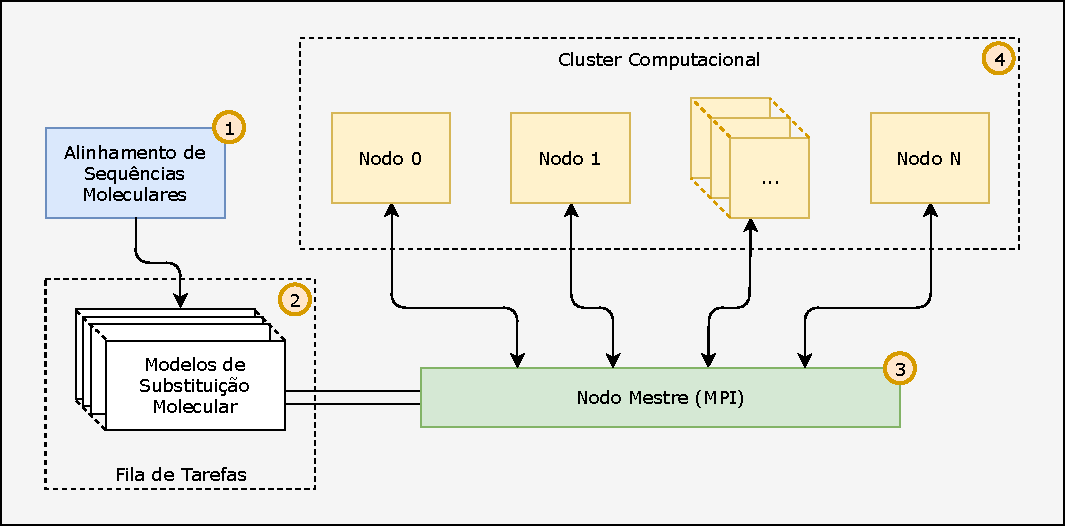
\includegraphics[width=\textwidth]{modelo-jmodeltest}
		\fonte{Adaptado de \citetexto{Darriba2014}.}
	\end{minipage}
	%\end{figure}
	%\begin{figure}[tb]
	%\centering%
	\begin{minipage}{.75\textwidth}
		\caption{Estratégia de paralelismo adotada pelo modelo \textsf{He}--lastic: um arquivo com múltiplas sequências moleculares alinhadas serve como entrada para um número de tarefas de avaliação (uma para cada sistema de substituição selecionado) que ficam, por sua vez, em uma fila de tarefas sendo primeiramente processadas na camada FaaS e encaminhadas para a camada de Orquestração de Contêineres em caso de falha por tempo de processamento expirado.}
		\label{fig:modelo-strategies}
		\vspace{1ex}
		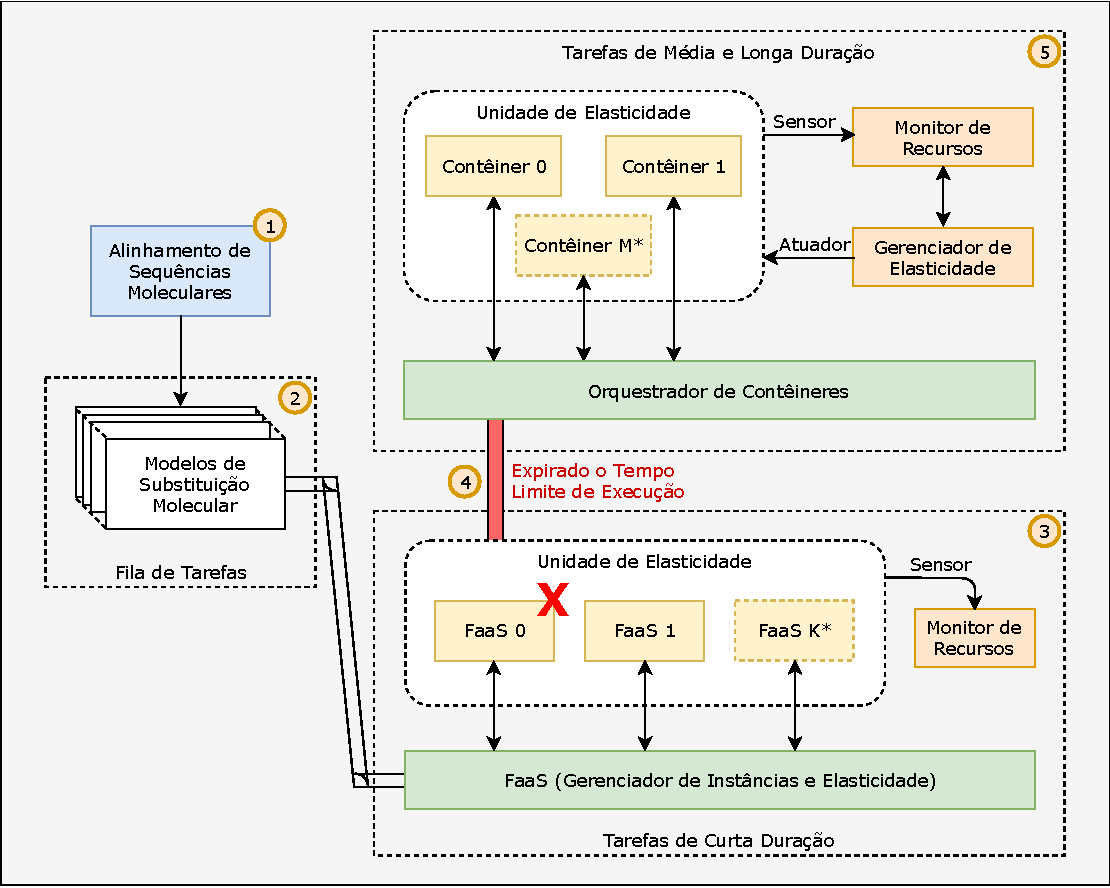
\includegraphics[width=\textwidth]{modelo-strategies}
		\fonte{Elaborado pelo autor.}
	\end{minipage}
\end{figure}



\begin{table}[tb]
	\centering%
	\begin{minipage}{\defaultFigureWidth\textwidth}
		\caption{Configuração do processamento efetuado pelo jModelTest durante o uso de \textit{Clustering Search} mostrando a quantidade e os sistemas de substituição molecular de acordo com a etapa.}
		\label{tab:modelo-elasticidade-jmodelsteps}
		\small
		\vspace{1ex}
		\renewcommand {\tabularxcolumn}[1]{>{\arraybackslash}m{#1}} % vertical center
		\begin{tabularx}{\textwidth}{rrX@{}}
			\toprule
			Etapa & Quantidade & {Sistemas} \\ 
			\midrule
			1 & 8 &  GTR, GTR+G, GTR+I, GTR+I+G, \newline SYM, SYM+G, SYM+I, SYM+I+G  \\
			2 & 120 &  001234~$\times~v$, 010234~$\times~v$, 011234~$\times~v$, 012034~$\times~v$, 012134~$\times~v$, 012234~$\times~v$, 012304~$\times~v$, 012324~$\times~v$, 012334~$\times~v$, 012340~$\times~v$, 012341~$\times~v$, 012342~$\times~v$, 012343~$\times~v$, 012344~$\times~v$, \newline TVM~$\times~v$, TVMef~$\times~v$  \\
			3 & 80 &  001203~$\times~v$, 010203~$\times~v$, 011203~$\times~v$, 012003~$\times~v$, 012103~$\times~v$, 012203~$\times~v$, 012300~$\times~v$, 012301~$\times~v$, 012302~$\times~v$, 012303~$\times~v$  \\
			4 & 48 &  001200~$\times~v$, 010200~$\times~v$, 011200~$\times~v$, \newline 012000~$\times~v$, 012100~$\times~v$, 012200~$\times~v$  \\
			5 & 24 &  000100~$\times~v$, 011000~$\times~v$, 011100~$\times~v$  \\
			6 & 8 &  JC, JC+G, JC+I, JC+I+G, \newline F81, F81+G, F81+I, F81+I+G  \\
			\bottomrule
			Total & 288 & \multicolumn{1}{r}{onde $ v~=~${\small \{ +F, +G, +G+F, +I, +I+F, +I+G+F, +I+G \}}} \\ 
		\end{tabularx}
		\fonte{Elaborado pelo autor.}
	\end{minipage}
\end{table}



Ao assumir um cenário de execução do jModelTest com um \textit{cluster} moderado para padrões atuais, contendo 64 \textit{cores} de processamento, haveria, em uma mesma execução, contenção por falta de recursos nas etapas dois e três, enquanto na etapa quatro, o ambiente teria uso de 75\% e nas demais apresentaria ociosidade significativa.
Através deste exemplo fica evidente o ganho que uma estratégia de elasticidade pode prover ao efetuar um casamento mais apropriado entre demanda e recursos disponíveis.
Desta forma, o modelo \textsf{He}--lastic lança mão da sua estratégia dividida em duas camadas de elasticidade para, ao mesmo tempo, otimizar para:
\begin{inparaenum}[\itshape a\upshape)] 
	\item a heterogeneidade na complexidade computacional, e consequente tempo de execução, para o cálculo de adequação de sistemas de substituição molecular; e
	\item a ampla variação na quantidade de recursos requeridos durante execução quando empregando o método de \textit{Clustering Search}; e
	\item manter um baixo impacto na eficiência (\textit{overhead}) comparado com a performance original do jModelTest. 
\end{inparaenum}


Comparada a abordagem original do jModelTest, representada pela \autoref{fig:modelo-jmodeltest}, a proposta do modelo \textsf{He}--lastic adiciona, na camada FaaS (de curta duração), um \textit{buffer} ou colchão, capaz de absorver uma parcela das requisições de forma paralela, enquanto evita sobrecarregar a camada de longa duração com alta rotatividade de tarefas.
Esta abordagem é ilustrada pela \autoref{fig:modelo-strategies}, onde encontram-se destacados cinco pontos de especial atenção, que detalham as semelhanças e distinções entre a abordagem jModelTest, sendo eles:

\begin{enumerate}[label={\arabic*)}]

	\item o programa recebe de entrada um arquivo contendo um conjunto de múltiplas sequências moleculares alinhadas, assim como no jModelTest;
	
	\item a partir dos parâmetros selecionados pelo usuário são geradas um conjunto de tarefas para execução do teste de adequação dos sistemas de substituição moleculares, assim como no jModelTest;
	
	\item através de filas de mensagens o componente FaaS, primeira camada de elasticidade e responsável pelas tarefas de curta duração, é notificado de que há processamento aguardando, o que serve como gatilho para que o provedor de computação em nuvem aloque os recursos necessários de maneira elástica, de forma que cada recurso seja responsável por processar uma única requisição;
	
	\item no caso em que um dos processamentos exceda o tempo limite de execução configurado para a camada FaaS, sua requisição é encaminhada para a segunda camada de elasticidade, o Orquestrador de Contêineres, onde são executadas as tarefas de média e longa duração;
	
	\item cada nodo da unidade de elasticidade recebe e processa múltiplas requisições, sendo elas testes de adequação de sistemas de substituição molecular, onde um gerenciador de elasticidade configurável pelo usuário/administrador dá conta de alocar e desalocar recursos, conforme os parâmetros de \textit{threshold} e a demanda, retornando uma lista de parâmetros numéricos que determina quão bem o sistema em questão representa os dados e os parâmetros que fizeram parte do teste de adequação.

\end{enumerate}


\section{Métricas de Avaliação}
\label{sec:modelo-metricas}



Uma vez definido o modelo \textsf{He}--lastic por meio das decisões que nortearam seu projeto, sua arquitetura e, principalmente, sua estratégia de elasticidade, resta detalhar como poderá ser avaliada sua performance e eficiência.
Esta seção dedica-se a esta tarefa, ao estabelecer e justificar métricas consideradas relevantes ao modelo e que possibilitam uma análise comparativa frente a possíveis alternativas e ao \textit{software} jModelTest.


Dado que o modelo \textsf{He}--lastic se origina de uma necessidade real baseada nas deficiências do projeto jModelTest no que diz respeito ao seu aproveitamento de recursos, é natural intuir que a análise de desempenho se dará através de execuções reais do \textit{software}, sendo este, efetivamente o caso.
Toda a avaliação do modelo \textsf{He}--lastic se dá por meio de execuções reais e que poderiam plenamente ser usadas por pesquisadores da bioinformática nas suas análises de inferência filogenética.


Contudo, ao contrário de abordagens que se apoiam em \textit{benchmarks} sintéticos, como o cálculo de aproximação para integrais ou o LINPACK de \citetexto{Dongarra2003}, o uso de avaliações reais impõem restrições no que diz respeito à definição do grão de paralelismo computacional.
Trabalhos como o de \citetexto{Kwiatkowski2002} comprovam a importância da escolha adequada da granularidade em cenários de computação paralela e distribuída, podendo este ser ajustado, no caso de avaliações sintéticas, facilmente através da regulagem dos parâmetros do algoritmo usado na computação.
Abordagens como a de \citetexto{Shankar2018}, que explora o paralelismo massivo das FaaS, mencionam especificamente a necessidade de ajustar a granularidade de tarefas para otimizar a computação:
\begin{quote}
	contanto que seja escolhida a granularidade de tarefas de forma que a maioria das tarefas possam ser concluídas com sucesso no intervalo de tempo alocado, não foi observada uma penalidade muito grande de desempenho pelo encerramento de um processo por conta do tempo limite de execução (\textit{timeout})
\end{quote}


Embora não seja possível, no caso do modelo \textsf{He}--lastic, controlar explicitamente o nível de granularidade, existem formas de fazer esta regulagem através dos parâmetros de execução do cálculo de adequação de sistemas de substituição de sequências moleculares.
Para este fim, são de grande valia o conjunto de equações detalhadas na \autoref{sec:modelo-arquitetura} que abordam o custo computacional em função do conteúdo do arquivo de múltiplos alinhamentos de sequências e os parâmetros da execução do teste de adequação, culminando na \autoref{eq:custo-jmodel-bestfit}.
Desta forma, para os fins deste trabalho, define-se a granularidade do paralelismo conforme:
\begin{quote}
	%TOD0: Definição é quando tens uma palavra ou expressão nova. Por exemplo: "granulosidade adaptativa"... - minha intenção era destacar alguns pontos determinantes pro entendimento das métricas de avaliação e resultados mais a frente. Acho que vou trocar para ‘decisões’ então. [gmail FMfcgxwBTsfLXGPKcBNKhxLncfDftgCR]
	\textbf{Premissa 1 --- da Granularidade:} a granularidade de uma execução do modelo \textsf{He}--lastic e, consequentemente, do \textit{software} jModelTest, pode ser determinada através da combinação entre o conteúdo do arquivo de múltiplos alinhamentos de sequências moleculares, fornecido como parâmetro de entrada, e os parâmetros escolhidos pelo usuário que determinarão, em última instância, quais sistemas de substituição farão parte do teste de adequação.
\end{quote}



De posse da definição de granularidade, útil tanto para o modelo \textsf{He}--lastic quanto para o jModelTest, há, ainda, a necessidade de estabelecer as métricas de performance.
Iniciando pelo jModelTest e seu modelo de computação distribuída de recursos fixos, o uso de uma formulação já existente se torna possível e recomendável com vistas a garantir a comparação com resultados similares.
Tomando por base as definições de Energia e Custo, regularmente utilizadas nas publicações oriundas do Programa de Pós--Graduação da UNISINOS, é possível especificar o Custo da execução do jModelTest, e por consequência, de recursos fixos, como sendo:

\begin{equation}
\label{eq:custo-jmodeltest}
Custo_{fixo}(t,j) = t \times j
\end{equation}
onde $ t $ representa o tempo total de execução e $ j $ representa a quantidade de \textit{cores} de processamento disponíveis.
A ausência de comportamento elástico garante uma formulação simples e direta, capaz de representar o custo do ponto de vista energético.
Uma vez que o presente trabalho também se interessa pelo custo financeiro da computação é relevante definir também a \autoref{eq:financeiro-jmodeltest} que se utiliza da \autoref{eq:custo-jmodeltest}:

\begin{equation}
\label{eq:financeiro-jmodeltest}
Financeiro_{fixo}(m,t,j) = m \times t \times j
\end{equation}
onde $ m $ representa o custo financeiro por unidade de tempo $ t $.



Visto que a elasticidade é central para a proposta do modelo \textsf{He}--lastic, devem ser definidas métricas análogas aquelas das Equações \ref{eq:custo-jmodeltest} e \ref{eq:financeiro-jmodeltest}.
Tendo em vista que a elasticidade é a capacidade de adicionar e remover recursos de maneira dinâmica de um ambiente de computação em nuvem, é necessária uma maneira de representar estes custos ao longo do tempo, onde a métrica de Energia adota uma abordagem análoga a um histograma, ao representar, ao longo de unidades de tempo $ pt_e $, que também pode ser interpretado como número de amostras, a quantidade de recursos disponíveis $ j $, no caso deste trabalho adotado como \textit{cores de processamento}, resultando na seguinte fórmula:

\begin{equation}
\label{eq:energia-elastico}
Energia(i,s) = \sum_{i=j}^{s} \big( j \times pt_e(j) \big) 
\end{equation}
sendo $ i $ e $ s $, respectivamente, os limites mínimo e máximo de \textit{cores} de processamento alocáveis durante a execução.
A \autoref{eq:energia-elastico} se transforma, por sua vez, na métrica de custo com a introdução tempo total de execução da aplicação:

\begin{equation}
\label{eq:custo-elastico}
Custo_{elastico}(t,i,s) = t \times Energia(i,s)
\end{equation}
onde, por fim, através da introdução do componente $ m $, que representa o custo financeiro por unidade de tempo $ t $, obtém-se a equação para o custo financeiro em cenários elásticos:

\begin{equation}
\label{eq:financeiro-elastico}
Financeiro_{elastico}(m,t,i,s) = m \times Custo_{elastico}(t,i,s)
\end{equation}



Embora as equações \ref{eq:energia-elastico}, \ref{eq:custo-elastico} e \ref{eq:financeiro-elastico} deem conta do cenário usual de elasticidade, elas se mostram insuficientes quando confrontadas com o cenário de elasticidade via FaaS, fundamental para a compreensão do modelo \textsf{He}--lastic.
Tendo por referência as características elencadas na \autoref{tab:FaaS-implementations}, apresentada na \autoref{sec:faas}, são necessários alguns ajustes para obter uma equação capaz de formalizar os conceitos de energia e custo no cenário FaaS, detalhados a seguir.



\begin{table}[tb]
	\centering%
	\begin{minipage}{\defaultFigureWidth\textwidth}
		\caption{Comparativo entre as principais variáveis que compõem a equação de Custo (\autoref{eq:custo-faas}) para o modelo FaaS de acordo com os limites impostos por três grandes provedores de computação em nuvem.}
		\label{tab:custo-faas}
		\small
		\vspace{1ex}
		\renewcommand\arraystretch{1.4}
		\renewcommand {\tabularxcolumn}[1]{>{\arraybackslash}m{#1}}
		\small
		\begin{tabularx}{\textwidth}{rYYYY@{}}
			\toprule
			& {AWS \textquoteleft18} & {AWS \textquoteleft17} & {Azure} & {GCP} \\ 
			\midrule
			$ y $ & $ 2 <= y <= 47 $ & $ 2 <= y <= 24 $ & $ 1 <= y <= 12 $ & $ y \in \{ 2, 4, 8, 16 \} $ \\
			\begin{tabular}[c]{@{}r@{}}$ F_{mem} $\\ (MB)\end{tabular} & 64 & 64 & 128 & 128 \\
			$ c $ & $ y $ & $ y $ & 1 & $ c \in \{ 1, 2, 4, 7, 12 \} $ \\
			\begin{tabular}[c]{@{}r@{}}$ F_{cpu} $\\ (MHz)\end{tabular} & 102 & 100 & 2400 & 200 \\
			$ t $ & $ <= 9000 $ & $ <= 3000 $ & $ <= 6000 $ & $ <= 5400 $ \\
			\begin{tabular}[c]{@{}r@{}}$ F_{tempo} $\\ (ms)\end{tabular} & 100 & 100 & 100 & 100 \\
			% \begin{tabular}[c]{@{}r@{}}\textit{cores} \\ disponíveis\end{tabular} & 2 caso $ y > 24 $, senão 1 & 2 caso $ y > 24 $, senão 1 & 1 & 1 \\
			\bottomrule
		\end{tabularx}
		\fonte{Atualizado pelo autor, adaptado de \citetexto{Wang2018}.}
	\end{minipage}
\end{table}


Em um primeiro momento é necessário descartar o conceito de Energia, uma vez que, no modelo FaaS, as execuções são contabilizadas individualmente e existe a alocação fracional de recursos, o que gera uma incompatibilidade com o a definição de Energia Elástica.
Em seguida, é necessário remodelar a definição de Custo, baseada na \autoref{eq:energia-elastico}, para que se ajuste à realidade observada durante o uso de FaaS, resultando em:

\begin{equation}
\label{eq:custo-faas}
Custo_{faas}(y,c,t) = \big( (y \times F_{mem}) \times (c \times F_{cpu}) \times (t \times F_{tempo}) \big)
\end{equation}
onde $ y $ e $ c $ são inteiros, ou então, serão arredondados para cima, representando, respectivamente: alocação de memória, alocação de CPU e tempo de execução.
Uma vez que cada um dos principais provedores de computação em nuvem estabelece limites e modelos de precificação diferentes, se torna relevante a visualização dos elementos contidos na \autoref{eq:custo-faas} na forma de uma tabela, como visto na \autoref{tab:custo-faas}.
Assim como a equação de custo financeiro para o cenário elástico se originou da definição de custo, o mesmo procedimento pode ser adotado no cenário de FaaS, resultando na seguinte equação:

\begin{equation}
\label{eq:financeiro-faas}
Financeiro_{faas}(m,y,c,t) = m \times Custo_{faas}(y,c,t)
\end{equation}
onde $ m $, tal qual na \autoref{eq:financeiro-elastico}, determina um componente de custo financeiro por unidade de tempo, podendo assumir um valor monetário como R\$ $ 5\text{,}25 $, \EUR{$ 1\text{,}5 $} ou \$ $2\text{,}75$, por exemplo.
Contudo, por convenção e padronização quanto às práticas de precificação adotadas pelos principais provedores de computação em nuvem, a unidade monetária adotada para $ m $ ao longo deste texto será o Dólar Americano~(\$), salvo indicação do contrário.



% COM OS 3 CUSTOS DÁ PRA UNIFICAR TUDO
Determinar uma métrica de avaliação unificada torna-se uma tarefa não trivial, considerando as particularidades, no que tange ao cálculo de Energia e Custo, conforme os modelos de execução por recursos fixos, com uso de elasticidade e com uso de FaaS.
Desta forma, mantendo-se fiel ao conceito de \textit{utility--computing} habilitado pela computação em nuvem, a métrica referente ao custo financeiro foi escolhida como fator de equalização entre os diferentes modelos de execução e será usada no restante deste trabalho.
Uma desvantagem em relação à métrica de custo financeiro está na sua variabilidade ao longo do tempo e entre provedores de computação em nuvem, uma vez que preços tendem a se alterar conforme são disponibilizadas novas funcionalidades e novos tipos de hardware.
\begin{quote}
	%TOD0: Definição é quando tens uma palavra ou expressão nova. Por exemplo: "granulosidade adaptativa"... - minha intenção era destacar alguns pontos determinantes pro entendimento das métricas de avaliação e resultados mais a frente. Acho que vou trocar para ‘decisões’ então. [gmail FMfcgxwBTsfLXGPKcBNKhxLncfDftgCR]
	\textbf{Premissa 2 --- da Métrica de Avaliação:} nos cenários que contemplem a composição entre múltiplos modelos de execução (fixo, elástico e FaaS), a métrica Financeira será utilizada como baliza para determinar as relações de eficiência. Tal definição se apoia na associatividade de custos, definida por \citetexto{Armbrust:EECS-2009-28}, ao afirmar que, em um ambiente de computação em nuvem usar 1000 máquinas por uma hora equivale a usar uma máquina por 1000 horas.
\end{quote}



Contudo, para os fins deste trabalho, esta desvantagem foi anulada através do uso de um único provedor de computação em nuvem e uma mesma família de hardware para as máquinas virtuais, decisões que são abordadas em detalhes na \autoref{sec:metodologia-infra}.
Ainda assim, a métrica de custo financeiro, além de ser um forma eficaz de prover uma linha justa de comparação entre as três abordagens, é resiliente por naturalmente conter em sua composição uma análise de energia e custo, ainda que realizada pelo provedor.
Resultando, enfim, nas definições 2 e 3:
\begin{quote}
	%TOD0: Definição é quando tens uma palavra ou expressão nova. Por exemplo: "granulosidade adaptativa"... - minha intenção era destacar alguns pontos determinantes pro entendimento das métricas de avaliação e resultados mais a frente. Acho que vou trocar para ‘decisões’ então. [gmail FMfcgxwBTsfLXGPKcBNKhxLncfDftgCR]
	\textbf{Premissa 3 --- do Provedor de Computação em Nuvem:} para os fins do presente trabalho fica estabelecida a restrição referente ao uso de um único provedor de computação em nuvem. Esta restrição não é imposta pelo modelo \textsf{He}--lastic, que é indiferente a uma possível implantação \textit{multi--cloud} em função da sua arquitetura desacoplada através de componentes independentemente escaláveis, contudo tem por objetivo manter uma comparação justa entre os diferentes modelos de execução, evitando discrepâncias no que tange à performance dos recursos computacionais subjacentes e à precificação dos mesmos.
\end{quote}
% FECHAMENTO


\section{Considerações Parciais}


Assim, elevando as capacidades da estratégia original do projeto jModelTest (\autoref{fig:modelo-jmodeltest}), o modelo proposto neste trabalho (\autoref{fig:modelo-strategies}) promove uma dupla camada de elasticidade:
\begin{inparaenum}[(i)]
	\item com o componente FaaS em um primeiro nível, absorvendo os picos de demanda e a parcela de requisições de curta duração, enquanto delega a gestão do ambiente e, principalmente, da elasticidade para o provedor de computação em nuvem evitando, assim, custos com ociosidade; e
	
	\item com o Orquestrador de Contêineres no segundo nível, provendo a capacidade necessária para a execução de tarefas de média e longa duração, enquanto reduz o esforço operacional e a complexidade da escolha dos parâmetros de elasticidade em função do seu uso reduzido, dado que parte dos cálculos poderá ser absorvida pela camada anterior.
\end{inparaenum}


Representando a principal contribuição do modelo proposto para o estado da arte, a divisão do tratamento de elasticidade em duas camadas (Figuras \ref{fig:modelo-arq-full}, \ref{fig:modelo-uml-activity}, \ref{fig:modelo-componentes-explodidos} e \ref{fig:modelo-strategies}) permite a adaptação às características computacionais do teste de adequação de sistemas de substituição de sequências moleculares, nomeadamente a irregularidade no esforço computacional dos cálculos (representado pela \autoref{fig:modelo-ociosidade}), enquanto reduz significativamente os custos com infraestrutura em comparação com a abordagem clássica de computação distribuída (baseada em \textit{clusters} ou \textit{grids}), conforme utilizada pelo projeto jModelTest (vide \autoref{fig:modelo-jmodeltest}).



Além disso, o modelo delega a gestão de tarefas secundárias\footnote{
	a expressão \textit{undifferentiated heavy--lifting} costuma ser usada no contexto de computação em nuvem para caracterizar tais esforços operacionais, sendo alguns exemplos, a configuração e manutenção de redes, \textit{firewalls} e segurança, aplicação de \textit{patches} e atualizações à nível de sistema operacional, entre outros.
} consequentemente reduzindo o fardo operacional enquanto se mantém agnóstico a provedores de computação em nuvem, permitindo amplas possibilidades de adoção tanto no meio acadêmico quanto comercial.
%
Como forma de possibilitar a comparação entre as abordagens do projeto jModelTest, assim como a elasticidade das camadas FaaS e de Orquestração de Contêineres, a métrica de avaliação selecionada neste trabalho é o custo financeiro, uma vez que ele se apresenta como denominador comum à todos os serviços de computação em nuvem.
%
A seguir o trabalho prossegue para especificar a metodologia de avaliação, fornecendo detalhes a respeito dos cenários de teste, as características do protótipo desenvolvido, assim como informações a respeito da aplicação e a infraestrutura de computação em nuvem utilizada.











\chapter{Metodologia de Avaliação}
\label{ch:modelo-metodologia}

\epigrafecap{Software maintenance is not \textquoteleft keep it working like before\textquoteright. \\ It is \textquoteleft keep being useful in a changing world\textquoteright.}{Jessica Kerr}



Neste capítulo é apresentada a metodologia empregada para avaliar o modelo proposto neste trabalho.
%
Por basear-se em um projeto de \textit{software} já desenvolvido e amplamente utilizado, o jModelTest, foi adotada uma abordagem de comparação entre o cenário atual, ou \textquoteleft o antes\textquoteright, com os cenários habilitados pelo modelo proposto, o \textquoteleft o depois\textquoteright.
%
Para tanto são definidos diversos cenários de avaliação capazes de exercitar as diferentes características dos projetos sob análise, assim como os parâmetros utilizados na execução.
%
Também são descritas neste capítulo as principais características da aplicação jModelTest e que influenciaram nas escolhas da metodologia de avaliação, assim como o ambiente de computação em nuvem e detalhes da implementação do protótipo desenvolvido neste trabalho.



Para realizar a avaliação do modelo \textsf{He}--lastic e futura comparação com o \textit{software} jModelTest foi desenvolvida uma aplicação à título de protótipo, que contemplasse na sua implementação as principais ideias e diferenciais propostos pelo modelo.
Todo código utilizado pelo protótipo, assim como o código do jModelTest, é publicamente acessível e encontra-se disponibilizado no portal GitHub, conforme apresentado na \autoref{tab:prototipo-repos}.


O protótipo foi desenvolvido utilizando a linguagem Python, na sua versão 3.6, no ambiente do provedor de computação em nuvem AWS, utilizando, portanto, suas APIs e serviços disponíveis como blocos de construção.
A abordagem adotada para replicar o funcionamento do jModelTest foi através da repetição de \textit{traces} de execução, o que exigiu pequenas modificações\footnote{
	As alterações realizadas para viabilizar a geração de \textit{traces} não alteraram o comportamento da aplicação e podem ser vistas no comparativo disponível no endereço: \url{https://github.com/mateusaubin/jmodeltest2/compare/8242fc..master?diff=split}.
} no projeto original.
Estas decisões são detalhadas a seguir.








\section{Etapas e Cenários}
\label{sec:metodologia-etapasecenarios}


\begin{table}[tb]
	\centering%
	\begin{minipage}{\textwidth}
		\caption{Repositórios contendo o código--fonte dos projetos utilizados na avaliação do modelo \textsf{He}--lastic.}
		\label{tab:prototipo-repos}
		\small
		\vspace{1ex}
		\renewcommand\arraystretch{1.4}
		\setlength{\tymin}{5em}
		\begin{tabulary}{\textwidth}{@{}CLL@{}}
			\toprule
			Repositório & Finalidade & Acessível em \\ 
			\midrule
			modeltest-lambda & Protótipo do modelo \textsf{He}--lastic & {\footnotesize \url{https://github.com/mateusaubin/modeltest-lambda}} \\
			
			modeltest-loadexerciser & \textit{Scripts} de execução dos cenários de avaliação e \textit{parsers} para coleta de estatísticas & {\footnotesize \url{https://github.com/mateusaubin/modeltest-loadexerciser}} \\
			
			\multirow{2}{*}{jmodeltest2} & Versão modificada para geração de \textit{traces} de execução & {\footnotesize \url{https://github.com/mateusaubin/jmodeltest2}} \\
			
			& Fontes originais do jModelTest & {\footnotesize \url{https://github.com/ddarriba/jmodeltest2}} \\
			
			PhyML & Motor de cálculo de adequação de sistemas de substituição molecular & {\footnotesize \url{https://github.com/stephaneguindon/phyml}} \\
			\bottomrule	
		\end{tabulary}
		\fonte{Elaborado pelo autor.}
	\end{minipage}
\end{table}

Visando fornecer uma rigorosa análise a respeito do modelo \textsf{He}--lastic, é necessário estabelecer uma base comum para que esta possa servir de comparação às futuras conclusões no que diz respeito ao modelo, seus modos de execução e as métricas detalhadas no \autoref{ch:modelo}.
A escolha dos dados utilizados para os testes é particularmente relevante para o cenário de comparação com o jModelTest em função dos fatores determinados na \autoref{list:fatores-influenciam-performance} e principalmente da \autoref{eq:custo-jmodel-bestfit}.


De posse dos dados, que servirão como bases aos cenários de testes, é possível iniciar na montagem e configuração de ambientes e na definição dos cenários de testes, tanto para o projeto jModelTest, quanto para o modelo \textsf{He}--lastic.
Por fim, os esforços são direcionados à coleta e análise dos dados obtidos através dos cenários de teste executados, sem deixar de lado a preocupação quanto a qualidade dos resultados obtidos, que deve ser avaliada por meio de análises estatísticas e de consistência, garantindo a pureza e relevância dos dados.


Este protocolo resulta em quatro etapas que dizem respeito ao processo de avaliação do modelo \textsf{He}--lastic, com a notável exceção sendo o desenvolvimento do protótipo que será abordado em detalhes nas próximas seções.
Abaixo são descritas as quatro etapas da avaliação e seus respectivos cenários:

\subsection{Parâmetros e Conjuntos de Dados}


\begin{table}[tb]
	\centering%
	\begin{minipage}{\defaultFigureWidth\textwidth}
		\caption{Conjuntos de dados utilizados na execução dos cenários de testes para o modelo \textsf{He}--lastic e o jModelTest.}
		\label{tab:metodologia-etapas-dataset}
		\vspace{1ex}
		\centering
		\begin{tabular*}{\textwidth}{@{\hspace{0.75em}}@{\extracolsep{\fill}}r@{~--~}lrrrr}
\toprule
\multicolumn{1}{c}{\#} & \multicolumn{1}{l}{Arquivo} & \multicolumn{1}{c}{Sequências} & \multicolumn{1}{c}{Comprimento} & \multicolumn{1}{c}{\begin{tabular}[c]{@{}c@{}}Quantidade \\ de Sistemas \\ de substituição\end{tabular}} & \multicolumn{1}{c}{\begin{tabular}[c]{@{}c@{}}Tempo\\ Total de \\ Execução\end{tabular}} \\ 
\midrule
01 & aP6 & 6 & 631 & 288 & 0:00:40 \\
02 & rodents & 8 & 1078 & 256 & 0:03:20 \\
03 & example & 10 & 1000 & 288 & 0:04:42 \\
04 & 18S\_insects2 & 7 & 902 & 256 & 0:04:52 \\
05 & HIVpol.groupM & 8 & 3009 & 256 & 0:11:58 \\
06 & Hex\_EF1a & 9 & 1092 & 256 & 0:20:12 \\
07 & primate-mtDNA & 12 & 898 & 288 & 0:24:23 \\
08 & HIV\_vpu.ref2 & 35 & 392 & 280 & 0:45:38 \\
09 & gusanos16S.mafft & 43 & 492 & 256 & 1:44:52 \\
10 & Birds & 9 & 14043 & 208 & 2:11:50 \\
11 & gusanosCOI.mafft & 44 & 561 & 256 & 2:58:49 \\
12 & stamatakis-59 & 59 & 6951 & 128 & 14:51:54 \\ 
\bottomrule
		\end{tabular*}
		\tabelafootnote{{*}~Tempo de execução obtido através da média das execuções do \textit{software} jModelTest realizando o teste de adequação para 288 sistemas de evolução em uma máquina com 2 processadores.}
		\fonte{Elaborado pelo autor.}
	\end{minipage}
\end{table}


\begin{table}[tb]
	\centering%
	\begin{minipage}{\defaultFigureWidth\textwidth}
		\caption{Parâmetros disponibilizados pelo jModelTest que influenciam diretamente na quantidade de sistemas de substituição molecular que farão parte do teste de adequação.}
		\label{tab:metodologia-etapas-jmodelparams}
		\small
		\vspace{1ex}
		\renewcommand\arraystretch{1.4}
		\setlength{\tymin}{9em}
		\begin{tabulary}{\textwidth}{CJ@{}}
			\toprule
			Parâmetro & Descrição \\ 
			\midrule
			Esquemas~de Substituição & Quantidade de sistemas de substituição molecular a ser incluídos no teste de adequação\textsuperscript{\dag} \newline 
			Opções disponíveis são \{3, 5, 7, 11, 203\} \\
			+F & Controla a inclusão de sistemas com frequências base iguais ou desiguais \\
			+I & Controla a inclusão de sistemas com ou sem uma proporção de locais invariantes em uma sequência molecular \\
			+G$_{n}$ & Controla a inclusão de sistemas com ou sem variação na taxa de substituição por local em uma sequência molecular \newline
			$n$ pode ser um número arbitrário que define a quantidade e categorias de variação \\
			\bottomrule	
		\end{tabulary}
	\tabelafootnote{{\textsuperscript{\dag}}~A \autoref{sec:modelos-de-substituicao} apresenta uma discussão detalhada a respeito dos sistemas de substituição, assim como a \autoref{tab:models} que apresenta alguns dos sistemas mais populares}
		\fonte{Elaborado pelo autor.}
	\end{minipage}
\end{table}


Esta etapa foi caracterizada por encontrar bases de dados padronizadas e amplamente utilizadas para testes no âmbito da filogenética, com o objetivo de estabelecer uma base comparativa que possa ser reproduzível por pesquisadores externos e que permita ampla avaliação do modelo proposto.
Estudos preliminares indicavam a existência de tais \textit{datasets}, conforme citam os trabalhos de \citetexto{Hordijk2005}, \citetexto{Keane2006a}, \citetexto{Stamatakis2005} e \citetexto{Stewart2001}, contudo alguns destes autores levantam dúvidas quanto a qualidade e padronização dos \textit{datasets}.


Através de comunicação pessoal por e-mail com Stamatakis e Darriba foi possível concluir que, de fato, não existem \textit{datasets} amplamente aceitos pela comunidade no que diz respeito à performance de testes de adequação de sistemas de substituição filogenética.
A recomendação recebida foi por utilizar os alinhamentos de exemplo que acompanham os binários do \textit{software} jModelTest, assim como elencar um subconjunto dos arquivos coletados em um repositório disponível no portal GitHub\footnote{
	Disponível na URL \url{https://github.com/stamatak/test-Datasets}.
}.
Embora exista uma quantidade significativa de alinhamentos presentes no repositório indicado, sua utilização se mostrou proibitiva em função do tempo de execução exigido e, consequentemente, a necessidade de um grande \textit{pool} computacional à disposição.


Tendo em vista que uma das diretrizes de projeto do modelo \textsf{He}--lastic está na sua capacidade de lidar com amplas variações no que diz respeito a carga computacional, o uso de arquivos que ultrapassem o tempo de execução de 24 horas foi julgado não relevante, uma vez que, do ponto de vista dos resultados, tais testes não adicionariam valor por apresentar comportamento muito similar dentre este conjunto.
A escolha por evitar alinhamentos de grandes dimensões também gera efeito no custo financeiro requerido para executar os cenários de testes do modelo e do jModelTest, além de contribuir significativamente no tempo necessário para executar cada cenário, de forma que a escolha por deixar tais arquivos de fora do conjunto de dados permitiu uma maior variação nos cenários de testes em função do tempo de execução reduzido.


Assim foram estabelecidos 12 arquivos com ampla variação no tempo de execução que serão usados para as execuções de avaliação do modelo \textsf{He}--lastic e do jModelTest.
Dos 12 arquivos apenas um deles se origina do repositório indicado por Stamatakis, enquanto os demais são oriundos do próprio projeto jModelTest.
Esta decisão foi motivada pelas circunstâncias expostas anteriormente e colhe apoio no fato de que favorece análises comparativas e facilita a avaliação dos resultados por terceiros.
A \autoref{tab:metodologia-etapas-dataset} apresenta os arquivos e algumas de suas características, assim como uma referência do tempo de execução máximo obtido por execuções em uma instância com dois núcleos de processamento disponíveis.


No que diz respeito aos parâmetros de execução das avaliações de adequação dos sistemas de substituição molecular, o objetivo principal é obter uma variedade que represente bem o cenário de um pesquisador da filogenética.
Conforme pode ser visto na \autoref{tab:metodologia-etapas-jmodelparams}, a escolha de sistemas de substituição está sob influência de quatro configurações disponibilizadas pelo \textit{software} jModelTest, onde o usuário pode selecionar quantidade de sistemas para teste e modificadores de comportamento.
Considerando este perfil de usuário foi estabelecido que os parâmetros de execução serão os mais compreensivos possíveis, empregando o maior número de avaliações para obter, desta forma, um amplo panorama acerca das características de execução de cada sistema de substituição molecular.


No jModelTest este cenário se dá através das utilização de \textit{Clustering Search}, conforme detalhado na \autoref{sec:estrategias-elasticidade}, que adota uma heurística capaz de reduzir os 1624 sistemas disponíveis para teste em 6 conjuntos que somados totalizam 288 sistemas (vide \autoref{tab:modelo-elasticidade-jmodelsteps}).
Também embasa esta escolha o fato de que parâmetros menos compreensivos de execução do jModelTest resultam em apenas 88, 40 ou 24 execuções paralelas, um número considerado baixo para colocar à prova as capacidades de paralelismo e elasticidade da camada FaaS do modelo \textsf{He}--lastic, uma vez que não é incomum encontrar servidores com mais de 16 \textit{cores} de processamento e VMs de provedores de computação em nuvem com mais de 30 núcleos.


Cabe ressaltar, mais uma vez, que a escolha dos arquivos de alinhamentos de sequências moleculares é particularmente relevante para o cenário de comparação com o jModelTest em função dos fatores determinados na \autoref{list:fatores-influenciam-performance} e, principalmente, através dos componentes da \autoref{eq:custo-jmodel-bestfit}, tornando o arquivo parte fundamental do grão de paralelismo juntamente com os parâmetros do jModelTest, detalhados na \autoref{tab:metodologia-etapas-jmodelparams}, que influenciam diretamente na escolha dos sistemas de substituição incluídos no teste dentre os 288 possíveis, como mostra a \autoref{tab:modelo-elasticidade-jmodelsteps}.



\subsection{Estratégia de Avaliação do jModelTest}


Para viabilizar uma comparação justa entre a abordagem de recursos fixos adotada pelo jModelTest, com a estratégia de elasticidade empregada pelo modelo \textsf{He}--lastic, existe a necessidade de coletar resultados de execução em um ambiente similar, reduzindo as variações em função de possíveis versões de dependências, modelos de hardware, situações de carga do ambiente e outras características inerentes a execução de softwares distribuídos e de alta performance.
Desta forma, a próxima etapa na avaliação do modelo consiste na execução do jModelTest com os arquivos e parâmetros, que determinam o grão de paralelismo, previamente selecionados em um ambiente similar ao que encontrará o protótipo do modelo \textsf{He}--lastic.


Este processo determinará o patamar básico de performance, também chamado de \textit{baseline}, que atua como balizador para os resultados oriundos do modelo proposto.
Apesar das diferenças no modelo de execução, as métricas coletadas nesta etapa são fundamentais para estabelecer uma linha de comparação quando confrontadas com os resultados obtidos pelo modelo \textsf{He}--lastic, exigindo, portanto, o mesmo rigor na execução e coleta dos resultados.


São fornecidos pelo \textit{software} jModelTest, dois modelos de execução paralela, sendo o primeiro deles baseado em memória compartilhada e \textit{threads} em um ambiente não distribuído, e o segundo adotando a biblioteca MPI como intermediador para a execução em \textit{clusters} ou \textit{grids} computacionais distribuídos.
Ambos os modos de execução estão disponíveis em um único binário desenvolvido, como indica o nome, na linguagem Java com a biblioteca MPJ Express \cite{Baker2006} constituindo a principal diferença entre eles.
Além disso, o programa permite tanto a execução através de console interativo via linha de comando, quanto por uma interface gráfica, o que segundo a \autoref{tab:survey-stats-comp} presente na análise do Estado da Arte realizada na \autoref{sec:analise-estadodaarte}, pode ser considerado um diferencial, haja vista que apenas 41\% dos trabalhos estudados contemplavam esta possibilidade.


Através de uma análise do código fonte é possível perceber que as funções de cálculo de adequação dos sistemas de substituição molecular são compartilhadas entre as quatro variantes de execução apresentadas, o que permite concluir que há uma significativa equivalência no esforço computacional entre elas, ainda que seja esperado um declínio na eficiência durante a operação baseada em MPI em função do \textit{overhead} de coordenação e comunicação entre os nodos do \textit{cluster}.


Durante a operação normal do jModelTest é possível observar dois comportamentos de execução, variando conforme a adoção ou não, da técnica de \textit{Clustering Search}, onde o modo que não utiliza esta técnica se comporta de maneira muito similar a um mestre--escravo ou até mesmo um \textit{scatter--gather}, embaraçosamente paralelo ao distribuir para cada nodo/processador um sistema de substituição de sequências para que seja executado o teste de adequação e agregando os resultados antes de devolver uma resposta ao usuário.
Nos casos onde há o uso de \textit{Clustering Search}, seu modo de operação se assemelha ao de fases paralelas (BSP), uma vez que existem seis fases de computação com barreiras, entre elas, que são utilizadas pela heurística para determinar o ponto de parada do algoritmo.
Embora não haja comunicação lateral entre os nodos de execução, sendo esta limitada a uma arquitetura mestre--escravo, a existência de uma barreira de sincronização é julgada suficiente para justificar a associação ao modelo BSP.
Este modo de execução pode gerar desperdício significativo de recursos em função da ociosidade ocasionada pela ampla variação no número de testes de adequação que são executados e, portanto, paralelizáveis em cada uma das 6 etapas que compõem a \textit{Clustering Search}, uma fraqueza do jModelTest já abordada na \autoref{sec:estrategias-elasticidade} e exemplificada na \autoref{tab:modelo-elasticidade-jmodelsteps}.


Para atender aos objetivos do presente trabalho foi selecionada a estratégia de execução baseada em \textit{threads} por memória compartilhada.
Esta decisão teve como objetivo coletar resultados do jModelTest em um cenário de \textit{overhead} mínimo, obtendo, assim, os melhores valores possíveis para a execução de cada um dos arquivos que compõem o \textit{dataset} de testes.
Uma comparação baseada na execução via MPI teria embutida em si todos os custos adicionais de comunicação, distribuição e coordenação entre nodos de processamento, contaminando os resultados.
Embora uma avaliação por este cenário possa ser desejável ao avaliar um sistema baseado em elasticidade, no contexto deste trabalho a execução de testes no cenário MPI incorreria em um elevado esforço de execução em função da configuração necessária para estabelecer um ambiente propriamente configurado e a dificuldade de automação desta tarefa, limitando, portanto, a capacidade de coleta de dados e confiabilidade dos resultados.


Outro fator que contribuiu para a escolha do cenário baseado em \textit{threads}, deve-se ao fato de que já é rotineiro encontrar disponível nos provedores de computação em nuvem VMs com quantidade de cores superior a 30, um número considerado suficiente para avaliar o impacto da estratégia de \textit{Clustering Search} na eficiência computacional, conforme variação no número de nodos de processamento disponíveis.
Através dos testes, adotando uma curva ascendente na quantidade de recursos disponíveis será possível, ao mesmo tempo que se determina um nível base de performance, verificar o impacto da estratégia \textit{Clustering Search} (e a variação no nível de paralelismo que ela causa, conforme a \autoref{tab:modelo-elasticidade-jmodelsteps}) na eficiência.


Conclui-se, portanto, que a avaliação do jModelTest e, consequente base comparativa para o modelo \textsf{He}--lastic se dará por meio da execução de múltiplas rodadas do teste de adequação em execuções em uma VM de cada vez, variando a quantidade de núcleos de processamento disponíveis, duplicando-os ou variando conforme disponibilidade do provedor de computação em nuvem, contemplando um intervalo aproximado de 2 à 40 \textit{cores}.
A \autoref{tab:metodologia-cenarios-jmodel} apresenta possíveis cenários de avaliação utilizando instâncias da família \texttt{c5}, disponível no provedor AWS com a nomenclatura $C_{zc}$, onde, $z$ representa jModelTest e $c$ o número de CPUs utilizadas.
Por meio desta estratégia serão obtidos dados mais otimistas possíveis, ao eliminar qualquer \textit{overhead} oriundo da computação distribuída e que permitirão estabelecer uma comparação rigorosa quanto ao consumo de recursos baseados em elasticidade do modelo \textsf{He}--lastic, além de, avaliar a atual eficiência no uso de tais recursos.
Os resultados obtidos por meio desta estratégia serão abordados em detalhes na \autoref{sec:resultados-jmodel}.


%threads é melhor porque é o caso mais eficiente (comparação mais exigente)
%mpi introduz custo de comunicação e complexidade no setup do ambiente (se mostrou proibitivo, dificil de automatizar)
%determinar o comportamento quanto ao aproveitamento de recursos, muito em função da clustering search
%resultados serão apresentados na \autoref{sec:resultados-jmodel}

\begin{table}[tb]
	\centering%
	\begin{minipage}{\defaultFigureWidth\textwidth}
		\begin{minipage}{.25\textwidth}
			\caption{Cenários de avaliação para o \textit{software} jModelTest.}
			\label{tab:metodologia-cenarios-jmodel}
			\vspace{1ex}
			\begin{tabularx}{\textwidth}{YW}
				\toprule
				Cenário & CPUs \\ 
				\midrule
				$C_{j2}$ & 2 \\
				$C_{j4}$ & 4 \\
				$C_{j8}$ & 8 \\
				$C_{j16}$ & 16 \\
				$C_{j36}$ & 36 \\
				\bottomrule
			\end{tabularx}
			\fonte{Elaborado pelo autor.}
		\end{minipage}
		\hfill
		\begin{minipage}{.65\textwidth}
			\caption{Cenários de avaliação para o modelo \textsf{He}--lastic.}
			\label{tab:metodologia-cenarios-helastic}
			\vspace{1ex}
			\small
			\begin{tabular*}{\textwidth}{lrlrr}
				\toprule
				& \begin{tabular}[c]{@{}r@{}}Orquestrador \\ de Contêineres\end{tabular} &  & \multicolumn{2}{c}{FaaS} \\
				\cmidrule{2-2}
				\cmidrule{4-5}
				Cenário & CPUs &  & Potência & Tempo Limite \\
				\midrule
				$C_{f0}$ & - &  & 1536 & 60 \\
				\addlinespace[1.5ex] 
				$C_{c8}$ & 8 &  & - & - \\
				$C_{c16}$ & 16 &  & - & - \\
				$C_{c36}$ & 36 &  & - & - \\
				\addlinespace[1.5ex] 
				$C_{m1}$ & 8 &  & 1536 & 60 \\
				$C_{m2}$ & 16 &  & 1536 & 45 \\
				$C_{m3}$ & 16 &  & 1536 & 60 \\
				$C_{m4}$ & 36 &  & 1536 & 15 \\
				$C_{m5}$ & 36 &  & 1536 & 30 \\
				$C_{m6}$ & 36 &  & 1536 & 60 \\
				$C_{m7}$ & 36 &  & 768 & 60 \\
				\bottomrule
			\end{tabular*}
			\fonte{Elaborado pelo autor.}
		\end{minipage}
	\end{minipage}
\end{table}








\subsection{Estratégia de Avaliação do \textsf{He}--lastic}
\label{sec:metodologia-etapas-modelo}

%%TODO: falar que até publicações reconhecidas decidiram empiricamente.
%\begin{verbatim}
%[Shankar2018]
%Ttimeout
%We use simple heuristics and empirical experiments to decide
%parameters, i.e., scaling factor s f and Ttimeout . We use simple heuristics and empirical experiments to decide
%these two parameters and leave more rigorous investiga-tion for future work. We set Ttimeout = 10s, which is the average start-up latency
%\end{verbatim}


A avaliação do modelo proposto se dará por meio da sua execução em ambiente computacional o mais próximo possível daquele onde se dará a coleta de métricas sobre o \textit{software} jModelTest, mantendo configurações de provedores de computação em nuvem, tipos e variedades de instâncias/VMs e sistemas operacionais.
Tais decisões visam maximizar a quantidade de variáveis controladas o que, por sua vez, reduz a incidência de ruídos ou influências indesejadas nos resultados coletados, visando comparação entre o modelo \textsf{He}--lastic e o jModelTest.
Conforme esperado, todos os testes devem ser executados com o mesmo conjunto de dados e parâmetros previamente definidos de forma que uma comparação justa possa se estabelecer entre as abordagens comparadas.



Os resultados obtidos nesta etapa tem a tripla finalidade de determinar:
\begin{inparaenum}[\itshape 1\upshape)] 
	\item a variação das métricas de avaliação comparadas às diferentes execuções do jModelTest;  
	\item o \textit{overhead} causado pela abordagem de camadas de elasticidade adotada pelo modelo proposto; e
	\item a variação de performance, conforme são desabilitadas as camadas do modelo.
\end{inparaenum}
Em última instância, os dados obtidos indicarão os pontos fortes e fracos da estratégia proposta, o que permitirá uma avaliação no que diz respeito a viabilidade da sua adoção, assim como um direcionamento quanto a possíveis trabalhos futuros em relação ao modelo \textsf{He}--lastic.


A flexibilidade do modelo proposto, através da sua dupla camada de elasticidade, se manifesta por meio dos parâmetros de configuração previamente detalhados na \autoref{tab:modelo-arq-params} especificando: 
\begin{inparaenum}[\itshape a\upshape)] 
	\item Tempo Limite;
	\item Potência;
	\item Número de CPUs;
	\item \textit{threshold} inferior; e
	\item \textit{threshold} superior,
\end{inparaenum} sendo os dois primeiros relevantes para a camada FaaS e os demais para a camada de Orquestração de Contêineres.
Contudo, esta flexibilidade acaba tornando-se um complicador ao estabelecer os cenários de testes, devido a explosão combinatória causada pelos cinco parâmetros do modelo, o que exige uma redução no espaço de busca para viabilizar a execução das avaliações.


No caso da camada baseada em FaaS, a associatividade de custos e proporcionalidade na alocação de recursos permite que as variações sejam concentradas em um dos dois parâmetros relevantes para esta camada, desta forma, o parâmetro de \textit{Timeout} (tempo limite de execução) será utilizado como principal elemento de variação, com a potência sendo usada para confirmar a associatividade de custos da camada FaaS.
Quanto a Orquestração de Contêineres foi definido que apenas o parâmetro relativo a quantidade de CPUs será variado, fixando-se os valores de controle do comportamento de elasticidade e alinhando o número de CPUs com aqueles adotados ao estabelecer as bases de comparação.
Esta decisão visa manter uma comparação justa entre os cenários ao reduzir a quantidade de variáveis que podem influenciar nos resultados e foi considerada adequada para determinar as características de comportamento do modelo \textsf{He}--lastic, haja vista, a grande quantidade de combinações possíveis entre \textit{thresholds}.


Contudo, a variação nos parâmetros do modelo não permite detectar os níveis de \textit{overhead} incorridos da sua utilização, requerendo uma abordagem alternativa para obtenção deste resultado.
Conforme detalhado na \autoref{sec:modelo-arquitetura}, o modelo \textsf{He}--lastic se diferencia em função da sua abordagem de duas camadas de elasticidade que, em função de suas características, se adéquam, em primeira análise, para diferentes tipos de aplicações, mas que, quando combinadas, podem contribuir para uma determinada classe de tarefas, como o teste de adequação de sistemas de substituição molecular.
Desta forma emergem três cenários de avaliação oriundos da combinação das camadas, nomeadamente os cenários: 
\begin{inparaenum}[\itshape 1\upshape)] 
	\item misto, contemplando ambas camadas habilitadas;  
	\item apenas FaaS; e
	\item apenas Contêineres.
\end{inparaenum}
Um quarto cenário, desabilitando ambas as camadas de elasticidade, embora possível, foi descartado por não ser relevante para o modelo proposto, uma vez que este é caracterizado pelo uso da elasticidade, assim, um cenário sem elasticidade forneceria uma caracterização deturpada do modelo \textsf{He}--lastic, além de exigir esforço de desenvolvimento e coleta de dados.


Os cenários elencados para avaliação do modelo são apresentados na \autoref{tab:metodologia-cenarios-helastic}, assim como um detalhamento a respeito dos valores atribuídos para cada um dos parâmetros relevantes à avaliação.
Tal como na \autoref{tab:metodologia-cenarios-jmodel}, o cenário assume trabalhar com instâncias do tipo \texttt{c5} do provedor AWS e sua nomenclatura segue o formato $C_{zc}$, onde $z$ pode assumir três valores \{FaaS, Contêineres, Misto\} e $c$ representa um sequencial à exceção dos cenários por Contêineres, onde representa o número de CPUs (que, por sua vez, está alinhado aos valores definidos previamente visando uma avaliação justa).
Merecem destaque, os cenários $C_{f0}$ e $C_{m7}$ por seus objetivos, sendo, respectivamente, examinar o ponto de limite no tempo de execução de tarefas e validar a associatividade de custos na camada FaaS, assim como, a proporcionalidade na alocação de recursos.
Os cenários $C_{c}$ têm por objetivo avaliar o nível de \textit{thrashing} e o \textit{overhead} causado pela execução de tarefas de curto prazo.
Por fim, os cenários $C_{m}$ colaboram para obter uma caracterização do comportamento dinâmico do modelo \textsf{He}--lastic no que diz respeito às camadas de elasticidade, além de medir sua eficiência.








\subsection{Análise Comparativa}


Uma vez obtidos os resultados referentes aos cenários de teste do jModelTest, assim como os do modelo \textsf{He}--lastic, a avaliação passa a se concentrar no estudo e comparação entre os resultados obtidos.
%
De posse dos dados brutos, conforme gerados pelo jModelTest, assim como pelo protótipo, estes serão compilados e tabulados para então passar por uma inspeção e limpeza, em busca de \textit{outliers}, de forma a evitar a ocorrência de viéses nos dados em função de anomalias, para que então possam servir como fontes adaptadas para análise.
%
Estas análises serão guiadas pelas métricas estabelecidas no \autoref{ch:modelo}, sendo de especial interesse os resultados relativos ao tempo total de execução e custo financeiro, que permitirão determinar os pontos fortes e fracos da proposta com relação à abordagem de recursos fixos adotada pelo jModelTest.
%
Além disso, também despertam interesse às características de elasticidade e a dinâmica de relacionamento entre as camadas FaaS e de Orquestração de Contêineres propostas pelo modelo \textsf{He}--lastic.









\section{Aplicação}


\begin{figure}[tb]
	\centering%
	\begin{minipage}{\textwidth}
		\caption{Linha de comando utilizada pelo jModelTest para controlar o \textit{software} PhyML separada em parcela fixa e variável e apresentando amostras de preenchimento da parcela variável.}
		\label{fig:prototipo-phyml-cmdline}
		\vspace{1ex}
		\begin{footnotesize}
			\textsf{\emph{Parcela Fixa:}}
			\begin{verbatim}
  -i arquivo.phy -d nt -n 1 -b 0 --r_seed 12345
  --no_memory_check -s BEST -o tlr
			\end{verbatim}
			\textsf{\emph{Parcela Variável:}}
			\begin{verbatim}
  --run_id GTR          -m 012345 -f m -c 1
  --run_id GTR+G        -m 012345 -f m -c 4 -a e
  --run_id GTR+I        -m 012345 -f m -v e -c 1
  --run_id GTR+I+G      -m 012345 -f m -v e -c 4 -a e
  --run_id F81          -m 000000 -f m -c 1 
  --run_id 001000       -m 001000 -f 0.25,0.25,0.25,0.25 -c 1
  --run_id 010200+I+G+F -m 010200 -f m -v e -c 4 -a e
  --run_id TIM1ef+I     -m 012230 -f 0.25,0.25,0.25,0.25 -v e -c 1
  --run_id TVM+G        -m 012314 -f m -c 4 -a e
  --run_id SYM          -m 012345 -f 0.25,0.25,0.25,0.25 -c 1
  --run_id SYM+G        -m 012345 -f 0.25,0.25,0.25,0.25 -c 4 -a e
  --run_id SYM+I        -m 012345 -f 0.25,0.25,0.25,0.25 -v e -c 1
  --run_id SYM+I+G      -m 012345 -f 0.25,0.25,0.25,0.25 -v e -c 4 -a e
			\end{verbatim}
		\end{footnotesize}
		\fonte{Elaborado pelo autor.}
	\end{minipage}
\end{figure}


Conforme já detalhado na \autoref{sec:modelo-selecao}, a aplicação que serve de base para a implementação do protótipo do modelo \textsf{He}--lastic é o jModelTest, um projeto já estabelecido no cenário de bioinformática e filogenética, que conta com amplo uso no meio acadêmico.
Seu objetivo é o cálculo de adequação de sistemas de substituição molecular, também conhecido como \textit{best--fit}, onde diversos sistemas de substituição são testados para determinar qual deles melhor explica as substituições moleculares que ocorreram em um determinado conjunto de dados.
Como resultado deste modo de operação, foi possível formalizar na \autoref{eq:custo-jmodel-bestfit} o cálculo referente a complexidade, ou custo computacional, de uma execução do jModelTest.
Outra característica relevante do projeto jModelTest, no que diz respeito ao protótipo, é a sua execução dividia em fases quando é utilizada a técnica de \textit{Clustering Search}, lembrando um algoritmo baseado em BSP, como é o caso dos cenários de avaliação estabelecidos para o presente trabalho.


Durante a implementação do protótipo foi possível explorar uma particularidade do jModelTest para obter o duplo benefício de agilizar o desenvolvimento e garantir a igualdade dos resultados, uma vez que o projeto atua basicamente como um \textit{driver} da aplicação PhyML de \citetexto{Guindon2010}.
Cada teste de adequação é mapeado para uma nova execução do PhyML, com os devidos parâmetros ajustados, embora mantendo uma estrutura base.
Sendo assim, é possível visualizar o jModelTest como um \textit{front--end} que dispara e gerencia múltiplas execuções paralelas do PhyML, recolhendo e compilando os resultados ao final delas.
A \autoref{fig:prototipo-phyml-cmdline} apresenta a parcela fixa da linha de comando utilizada para controlar o comportamento do PhyML, assim como, exemplos da parcela variável que são, por fim, combinadas para gerar cada linha de comando que dispara a execução de um teste de adequação de sistemas de substituição molecular.


Em função da relação entre jModelTest e PhyML é possível basear a implementação do protótipo no \textit{replay} dos comandos enviados ao PhyML, bastando para isso a coleta de \textit{traces} de execução.
Estes registros foram habilitados pelo autor por meio de uma versão levemente modificada do jModelTest, e que permitiu garantir o mesmo comportamento no que diz respeito à característica das execuções, haja vista que o cálculo de adequação, realizado pelo PhyML, é a parte mais custosa da execução do jModelTest.
Os arquivos de trace encontram-se disponíveis no repositório\footnote{
	Disponível no endereço: \url{https://github.com/mateusaubin/modeltest-loadexerciser/tree/master/traces}
} que armazena o código fonte dos \textit{scripts} de execução.


Uma das tarefas realizadas pelo jModelTest, para viabilizar a comunicação com o PhyML, é a conversão nos tipos de arquivo fornecidos como parâmetros de entrada.
Uma vez que o protótipo também funcionará como um controlador do PhyML, existe a necessidade de converter os tipos de dados dos arquivos utilizados no \textit{dataset} de avaliação do modelo.
Para tanto, foi utilizada a biblioteca ALTER, especializada na conversão entre tipos de alinhamentos e também utilizada pelo jModelTest, de modo que todos os arquivos presentes no \textit{dataset} estejam em formato .phy, que é o único reconhecido pelo PhyML.


Visando obter uma maior qualidade e reprodutibilidade das execuções realizadas, a aplicação contou com automação, por meio de scripts de execução automatizada dos cenários, tanto para estabelecer as bases de comparação no jModelTest\footnote{Disponível no endereço: \url{https://github.com/mateusaubin/modeltest-loadexerciser/blob/master/exec-old-userdata.sh}}, quanto para gerir e executar as execuções do protótipo do modelo \textsf{He}--lastic\footnote{
	Disponível nos endereços: \url{https://github.com/mateusaubin/modeltest-loadexerciser/blob/master/exec-new.py}
	\&
	\url{https://github.com/mateusaubin/modeltest-loadexerciser/blob/master/exec-new-helper.sh}
}. 
Através da automação foi possível aumentar o número de execuções de cada cenário de avaliação e, consequentemente, a confiabilidade estatística dos resultados.
Outro benefício da automação foi possibilitar a execução não assistida dos cenários, o que teria comprometido seriamente a capacidade de execução, uma vez que, múltiplos cenários ultrapassavam a marca de 20 horas de execução para todos os arquivos contidos no \textit{dataset} de testes e estes, por sua vez, deveriam ainda ser repetidos ao menos cinco vezes.







\section{Infraestrutura}
\label{sec:metodologia-infra}


\begin{figure}[tb]
	\centering%
	\begin{minipage}{\defaultFigureWidth\textwidth}
		\caption{Mapa das regiões e respectivas zonas de disponibilidade fornecidas pelo provedor de computação em nuvem AWS, com os círculos verdes representando regiões em construção.}
		\label{fig:metodologia-infra-awsregions}
		%	\vspace{1ex}
		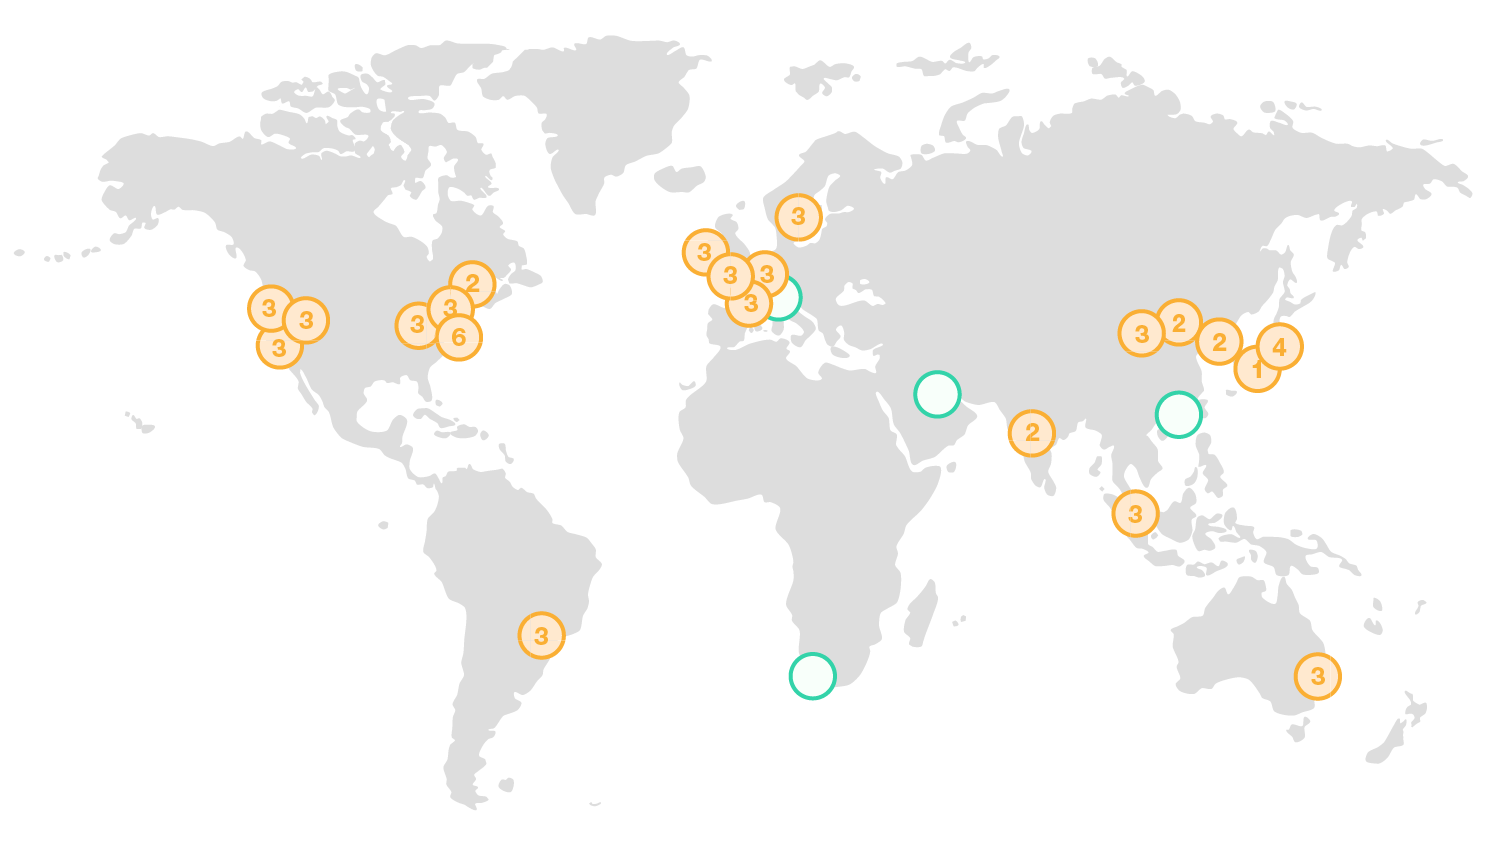
\includegraphics[width=\textwidth]{aws-regions}
		\fonte{Reproduzido de {\scriptsize \url{https://aws.amazon.com/about-aws/global-infrastructure/}}.}
	\end{minipage}
\end{figure}

%\afterpage{
\begin{figure}
	\centering%
	\begin{minipage}{.49\textwidth}
		\caption{Variação no custo por região do provedor AWS no uso de recursos computacionais em instâncias da família \texttt{m5}.}
		\label{fig:metodologia-infra-cost-compute}
		%	\vspace{1ex}
		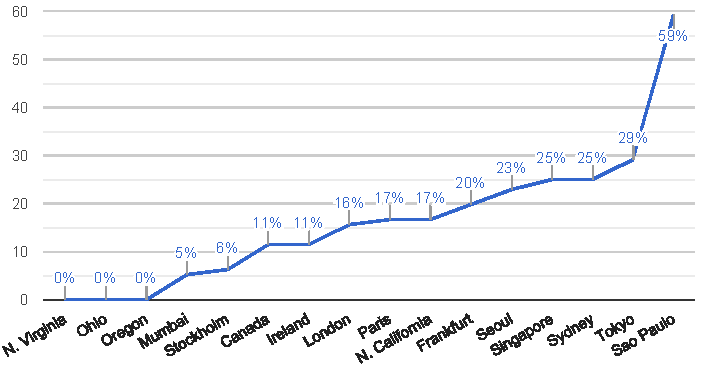
\includegraphics[width=\textwidth]{aws-compute-costperregion}
		\fonte{\citetexto{AWSRegionCost}.}
	\end{minipage}
	\hfill
	\begin{minipage}{.49\textwidth}
		\caption{Variação no custo por região do provedor AWS para a transferência de 1 TB de dados para a Internet.}
		\label{fig:metodologia-infra-cost-network}
		%	\vspace{1ex}
		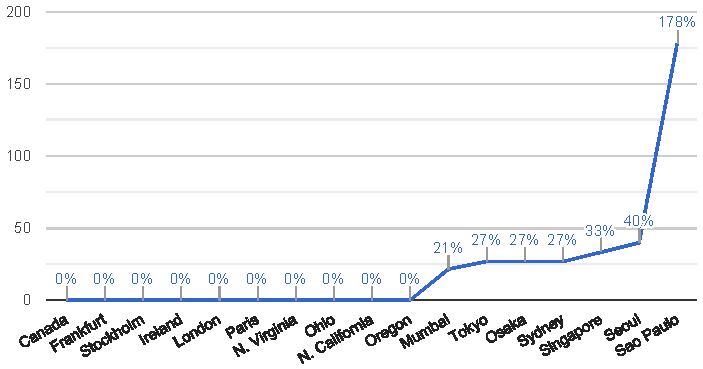
\includegraphics[width=\textwidth]{aws-network-costperregion}
		\fonte{\citetexto{AWSRegionCost}.}
	\end{minipage}
\end{figure}
%}

No que diz respeito a infraestrutura de computação em nuvem, a escolha foi pelo provedor Amazon Web Services (AWS), uma subsidiária da Amazon, que por sua vez, é considerada uma gigante do \textit{e-commerce} nos Estados Unidos e já conta com alguma atuação no Brasil.
%
A escolha da AWS se deu por este ser o maior dentro os grandes provedores de computação em nuvem (também chamados na imprensa de \textit{hyperscalers}) e por experiência acadêmica e profissional do autor que usou e administrou nos quatro anos anteriores ambientes de nuvem baseados no provedor AWS, além de utilizá-lo como plataforma para o desenvolvimento do projeto Elastipipe, realizado como trabalho de conclusão na Graduação \cite{Aubin2015,Aubin2016,Aubin2017}.
%
A arquitetura do provedor é baseada em regiões, sendo estas geralmente divididas à nível continental onde cada região é, por sua vez, subdividida em pelo menos duas (ou geralmente três) zonas de disponibilidade, conforme mostra a \autoref{fig:metodologia-infra-awsregions}.


As zonas de disponibilidade servem como proteção contra desastres e mecanismo de redundância e alta disponibilidade, por representarem ambientes espelhados umas das outras, no que diz respeito à infraestrutura do provedor.
%
Contudo, para tirar proveito dessas capacidades, geralmente é necessário que a aplicação seja preparada para saber lidar com esta possibilidade.
%
Embora as regiões costumem ser parecidas, existe entre elas certa diferença no rol de serviços ofertados e, por vezes, até mesmo no hardware disponível, o que pode complicar a escolha.
%
Um exemplo disso, foi a recente chegada do serviço \textit{Redshift} na região situada em \texttt{sa-east-1} (São Paulo, Brasil) no fim de 2016, sendo que sua oferta inicial na região \texttt{us-east-1} (Virgínia do Norte, USA) ocorreu em 2012.


No contexto deste trabalho, a região escolhida foi a \texttt{us-east-2} localizada em Ohio, USA, com os principais motivadores sendo custo e funcionalidades, pois a região brasileira ainda não disponibiliza parte significativa\footnote{
	A página \url{https://aws.amazon.com/about-aws/global-infrastructure/regional-product-services/} apresenta a lista completa de serviços disponível por região e permite chegar a esta conclusão.
}
do portfólio de serviços da AWS, além de cobrar um preço mais alto pelo uso dos recursos, resultando em um \textit{premium} de pelo menos 50\% sobre o valor base cobrado em Ohio, segundo levantamento de \citetexto{AWSRegionCost}, demonstrado nas Figuras \ref{fig:metodologia-infra-cost-compute} e \ref{fig:metodologia-infra-cost-network}.
%
A política de preços é relevante na escolha da região, pois, embora esteja situada no Brasil, a cobrança dos custos oriundos desta região ainda se dá em Dólares Americanos (USD), assim como todas as demais regiões, o que nega qualquer benefício fiscal e/ou tecnológico advindo do seu uso (uma exceção seria o desenvolvimento de aplicações altamente sensíveis a latência, por exemplo).


O pioneirismo da AWS, no que diz respeito ao paradigma FaaS / \textit{serverless}, também teve grande influência na escolha, haja vista, que foi este provedor quem efetivamente deu origem a este modelo computacional.
Medições realizadas por \citetexto{McGrath2017} indicam que a AWS fornece as melhores métricas em termos de escalabilidade, latência de arranque frio (\textit{coldstart}) e taxa de transferência.
Além destes resultados, testes realizados por \citetexto{Wang2018} concluem que o serviço provido pela AWS é superior, uma vez que plataformas concorrentes como Azure, da Microsoft, e GCP, da Google, enfrentam dificuldades em provisionar um número suficiente de recursos subjacentes, capazes de servir requisições com alto paralelismo.
Enquanto este comportamento é geralmente visto como vantagem, este resultado se dá em função da política de \textit{bin--packing}, adotada pela AWS, que tenta manter o melhor aproveitamento de recursos servindo requisições FaaS a partir das mesmas VMs, até que não haja mais espaço, onde só então é provisionada uma nova VM.
Contudo, \citetexto{Wang2018} previnem que esta política pode resultar em contenção, conforme as características no uso de recursos por parte das funções executadas, podendo prolongar artificialmente o tempo de execução.


\begin{table}[b]
	\centering%
	\begin{minipage}{\defaultFigureWidth\textwidth}
		\caption{Tipos de CPUs utilizadas no AWS Lambda e sua equivalência em termos de Famílias EC2.}
		\label{tab:metodologia-infra-lambdacpus}
		%\small
		\vspace{1ex}
		%		\renewcommand\arraystretch{1.4}
		\begin{tabularx}{\textwidth}{@{}WYYYY@{}}
			\toprule
			Fração\textsuperscript{\dag} & vCPU & Frequência & Denominação & Família \\ \midrule
			59,3~\% & E5-2666 & 2,90~GHz & Haswell & \texttt{c4} \\
			37,5~\% & E5-2680 & 2,80~GHz & Ivy Bridge & \texttt{c3} \\
			3,1~\% & E5-2676 & 2,40~GHz & Haswell & \texttt{m4} \\
			\bottomrule	
		\end{tabularx}
		\tabelafootnote{\textsuperscript{\dag}~~Levantamento realizado através da coleta de estatística dos arquivos /proc/cpuinfo e /proc/meminfo de 20 mil VMs distintas.}
		\fonte{\citetexto{Wang2018} com complementos do autor.}
	\end{minipage}
\end{table}


Uma das vantagens para o provedor, no que diz respeito ao uso de FaaS (abordada na \autoref{sec:faas}), está na possibilidade de manter um bom nível de utilização para hardware que esteja caindo em desuso.
Havendo a possibilidade de manter um determinado patamar de performance entre diferentes VMs e famílias de instâncias, as limitações no consumo de recursos estabelecidas pelo paradigma FaaS permitem com que versões relativamente antigas de hardware sejam utilizadas sem desvantagens ao usuário, ao mesmo tempo que reduz a necessidade de compra para o provedor.
Este comportamento pode ser observado na \autoref{tab:metodologia-infra-lambdacpus} que apresenta a distribuição de frequência com que são utilizados determinados tipos de CPUs no AWS Lambda, a oferta de FaaS do provedor AWS, em comparação com o uso destas mesmas CPUs quando disponíveis no serviço de máquinas virtuais, o EC2.
Para referência, famílias atuais do EC2 são aquelas que têm sufixo \texttt{5}, como por exemplo, \texttt{c5}, \texttt{r5} e \texttt{m5}, que são otimizadas para CPU, memória e uso geral, respectivamente.



A ampla seleção de serviços disponibilizados pela nuvem da AWS faz com que o exercício e definição de arquitetura se assemelhe a montagem de LEGO\footnote{
	Brinquedo infantil caracterizado por suas peças que se encaixam e permitem montar uma infinidade de objetos.
}
onde é possível deixar a cargo do provedor diversas das funcionalidades fundamentais de um projeto \textit{software}.
Visando garantir o entendimento da arquitetura do protótipo descrita a seguir, uma lista com os serviços mais relevantes utilizados é apresentada abaixo, juntamente com uma breve descrição de suas características e funcionalidades.


\begin{itemize}
	
	\item \textbf{Lambda:} é a implementação da AWS para o paradigma FaaS;
	
	\item \textbf{Batch:} serviço para execução de tarefas em modo \textit{batch} de processamento, provendo mecanismos de filas, prioridades e ambientes de computação, além de gerenciar automaticamente ações de elasticidade conforme a demanda;
	
	\item \textbf{S3:} provê armazenamento de objetos/arquivos com alta capacidade de requisições e \textit{throughput}, enquanto fornece garantias de replicação e durabilidade de 11 noves;
	
	\item \textbf{DynamoDB:} banco de dados não relacional (NoSQL) orientado a tuplas chave--valor com latência na casa de um dígito de segundo ($0\sim9$s);
	
	\item \textbf{SNS:} filas de mensagens no modelo \textit{publish--subscribe} suportando alta vazão e durabilidade por meio de servidores distribuídos, fornecendo política de entrega \textquoteleft pelo menos uma vez\textquoteright (\textit{at least once delivery});
	
	\item \textbf{ECS:} é a implementação da AWS para o paradigma de Orquestração de Contêineres, sendo utilizado como recurso subjacente pelo Batch, para viabilizar a execução de qualquer tipo de aplicação em um ambiente isolado e com todas as dependências embutidas por meio de contêineres Docker;
	
	\item \textbf{Auto--Scaling:} mecanismo de elasticidade fornecido pela AWS, que possibilita a definição de regras para elasticidade horizontal automática e reativa por replicação de VMs (\autoref{fig:elasticidade-taxonomia}), sendo utilizado pelo ECS no controle da elasticidade;
	
	\item \textbf{EC2:} base para a grande maioria dos demais serviços providos pela AWS, fornecendo, também para usuários finais, Máquinas Virtuais configuráveis em uma ampla variedade de dimensões como processamento, memória, endereços de IP e placas de rede, armazenamento e imagens de sistemas operacionais;
	
	\item \textbf{CloudWatch:} coleta, gestão e relatórios de métricas operacionais gerads pelos demais serviços AWS e pelo próprio usuário;
	
	\item \textbf{CloudFormation:} gerencia a montagem, atualização e remoção de ambientes computacionais definidos por meio de uma linguagem de programação, aplicando o conceito conhecido como \textit{infrastructure as code};
	
	\item \textbf{IAM:} gestão e permissionamento de usuários, grupos e papéis.
	
\end{itemize}



%[Shankar2018]
%cloud providers
%also offer publish-subscribe services like Amazon SQS
%or Google Task Queue. These services typically do not
%support high data bandwidths but can be used for “con-trol plane” state like a task queue that is shared between
%all serverless function invocations. Providers often of-fer consistency guarantees for these services, and most
%services guarantee at least once delivery.
%
%[Shankar2018]
%runtime state store.
%--- É O MEU DYNAMODB

% -----------



% https://github.com/lambci/docker-lambda
%https://www.bbva.com/en/economics-of-serverless/

% http://www.perrygeo.com/running-python-with-compiled-code-on-aws-lambda.html - talvez não relevante









\section{Protótipo}


Desenvolvido na linguagem de programação Python, o protótipo do modelo \textsf{He}--lastic tira proveito do fato de que o jModelTest atua como \textit{front--end} para o PhyML e adota uma estratégia baseada na reexecução de \textit{traces} coletados a partir de uma versão do jModelTest modificada para gerar tais registros.
%
Conforme mencionado anteriormente, o uso do PhyML como efetivo executor dos cálculos necessários para o teste de adequação de sistemas de substituição molecular é a tarefa mais custosa computacionalmente, de forma que, o uso de \textit{traces} não foi considerado uma vantagem para o protótipo, por não tomar, no jModelTest, tempo suficiente de cálculo, para ser significativo na avaliação de tempos de execução.
%
Além disso, o uso do PhyML provê um segundo benefício, ao garantir que os cálculos executados pelo protótipo são exatamente os mesmos do que aqueles desempenhados pelo jModelTest, validando os resultados e assegurando que as diferenças nos custos e tempos de execução se originam, exclusivamente, das diferenças entre o modelo \textsf{He}--lastic (e seus modos de execução) e do jModelTest.








\subsection{Implementação}


Uma das diretivas que guiou o desenvolvimento foi a adoção do maior número possível de serviços de computação em nuvem, onde fosse possível e apropriado, resultando em um desenvolvimento efetivamente \textit{cloud--native}, buscando maximizar a performance e a obter tolerância a falhas necessária para aplicações distribuídas e de alto desempenho.
%
Esta decisão está alinhada com as decisões de projeto detalhadas na \autoref{list:decisoes-de-projeto} e tem como subproduto uma simplificação na configuração, assim como, a consequente redução na carga operacional do administrador de ambientes.
%
No que diz respeito a portabilidade entre provedores de computação em nuvem, todos os serviços fundamentais encontram concorrentes com funcionalidades análogas, enquanto serviços secundários, nomeadamente CloudWatch, CloudFormation e IAM, também têm concorrentes, contudo, sua adaptação requer intervenção manual devido às diferenças e características de cada plataforma de computação em nuvem.


\begin{table}[tb]
	\centering%
	\begin{minipage}{.8\textwidth}
		\caption{Artefatos de código presentes nos três módulos do protótipo.}
		\label{tab:metodologia-prototipo-artefatos}
		\vspace{1ex}
		% sequential 4-class Blues reversed
		\definecolor{c1}{HTML}{6baed6}%
		\definecolor{c2}{HTML}{bdd7e7}%
		\definecolor{c3}{HTML}{eff3ff}%
		%
		\begin{tabularx}{\textwidth}{
				>{\hsize=0.9\hsize}X
				>{\hsize=0.9\hsize}X
				>{\hsize=1.2\hsize}X
			}
			\toprule
			\multicolumn{2}{c}{FaaS} & \multicolumn{1}{c}{\multirow{2}{*}[-0.5\dimexpr \aboverulesep + \belowrulesep + \cmidrulewidth]{\begin{tabular}[c]{@{}c@{}}Orquestrador de\\ Contêineres\end{tabular}}} \\ 
			\cmidrule(lr){1-2}
			\multicolumn{1}{c}{\texttt{forwarder}} & \multicolumn{1}{c}{\texttt{modeltest}} & \multicolumn{1}{c}{} \\ 
			\midrule
			\rowcolor{c1} 
			src/aws.py & src/aws.py & src/aws.py \\
			src/forwarder.py & \cellcolor{c2} lib/phyml & \cellcolor{c2}lib/phyml \\
			& \cellcolor{c3} src/modeltest.py & \cellcolor{c3} src/modeltest.py \\
			&  & src/dockerentrypoint.py \\
			&  & requirements.txt \\ 
			\bottomrule
		\end{tabularx}
		\fonte{Elaborado pelo autor.}
	\end{minipage}
\end{table}


Um dos destaques do ponto de vista da implementação do protótipo do modelo \textsf{He}--lastic, e que pode ser observado nos repositórios públicos de código fonte listados na \autoref{tab:prototipo-repos}, foi o alto índice de reuso de código, uma propriedade que emergiu em função da utilização das duas camadas de elasticidade baseadas em FaaS e Contêineres, onde o código utilizado como função na camada FaaS foi inteiramente compartilhado com a camada de Contêineres, na forma de uma biblioteca de código fonte.
%
Embora a camada de Contêineres não faça uso ou referencie da camada FaaS, o código fonte compartilha exatamente o mesmo artefato que foi enviado para a camada FaaS, necessitando apenas de um \textit{wrapper} capaz de traduzir as estruturas de dados para que fiquem no formato esperado pela chamada da função.
%
Os módulos desenvolvidos no protótipo, assim como, seus artefatos de código podem ser vistos na \autoref{tab:metodologia-prototipo-artefatos}, onde também é possível visualizar o alto nível de reuso de código por meio do uso do PhyML, da biblioteca de funções \texttt{aws.py} e do executável \texttt{modeltest.py}.


Embora fossem esperados apenas dois programas, sendo um para cada camada do modelo, houve a necessidade durante o desenvolvimento de produzir três programas, para que o protótipo pudesse funcionar conforme especificado na arquitetura do modelo, seguindo as definições da \autoref{sec:modelo-arquitetura}.
%
A diferença deu-se pela necessidade de introduzir um módulo responsável por traduzir as requisições originalmente enviadas para a camada FaaS (Lambda), em requisições que seguissem o formato especificado para a camada de Contêineres (Batch), originando o módulo \textit{\texttt{forwarder}}.
%
Este módulo tem seu objetivo estritamente definido pelo encaminhamento de requisições, não realizando qualquer tipo de cálculo ou computação útil do ponto de vista do teste de adequação de sistemas de substituição molecular, contudo, cumprindo um papel necessário para o funcionamento do protótipo.
%
Em contrapartida, realizam processamentos úteis, do ponto de vista funcional, os módulos \textit{\texttt{modeltest}} na camada FaaS, e o respectivo módulo da camada Orquestradora de Contêineres que, conforme mencionado, reutiliza totalmente código do módulo anterior.







\subsection{Ferramental}
Dentre o ferramental adotado para o desenvolvimento do protótipo, o projeto Docker contribuiu de maneira significativa para garantir a testabilidade do protótipo ao permitir a especificação de um ambiente isolado e bem definido contendo os artefatos de código, \textit{runtimes} e dependências empacotadas em uma única imagem, que pode ser utilizada no ambiente de Orquestração de Contêineres (Batch) e localmente.
%
Através de um arquivo chamado \texttt{dockerfile} é possível especificar todos os passos necessários para a construção do contêiner e obter, depois de compilado, uma imagem pronta para implantação em qualquer ambiente que suporte imagens Docker.
%
Além disso, por meio de projetos como o docker-lambda\footnote{
	Disponível em \url{https://github.com/lambci/docker-lambda}.
} é possível obter localmente um ambiente que reproduz as características da camada FaaS (Lambda), o que também contribuiu para a testabilidade e o desenvolvimento do protótipo.


O projeto \textit{serverless framework}\footnote{
	Disponível em \url{https://serverless.com/framework}.
}, que fornece uma visão unificada a respeito das capacidades de FaaS disponíveis nos principais provedores de computação em nuvem, também teve papel fundamental no desenvolvimento do protótipo e possibilitou mantê-lo agnóstico de provedores.
%
Através do arquivo \texttt{serverless.yml} foi possível especificar todo o ambiente computacional necessário para a execução do protótipo, contemplando as duas funções FaaS e suas configurações, assim como o Orquestrador de Contêineres e suas respectivas configurações.
%
Esta capacidade está intimamente ligada ao fato de que o \textit{serverless framework} permite ao usuário embutir comandos CloudFormation no processo de implantação (\textit{deployment}) do projeto, de maneira que o arquivo \texttt{serverless.yml} define tudo o que diz respeito à criação, atualização e remoção do ambiente requerido pelo protótipo do modelo \textsf{He}--lastic, permitindo com que simples comandos como \texttt{\textit{sls deploy}} e \texttt{\textit{sls remove}} montem e desmontem todos os componentes necessários para a execução, assim como suas dependências.






\subsection{Arquitetura do Protótipo}


\begin{figure}[tp]
	\centering%
	\begin{minipage}{\textwidth}
		\caption{Diagrama de arquitetura da implementação do protótipo do modelo \textsf{He}--lastic descrevendo as principais etapas no fluxo de execução.}
		\label{fig:metodologia-prototipo-arquitetura}
		\vspace{1ex}
		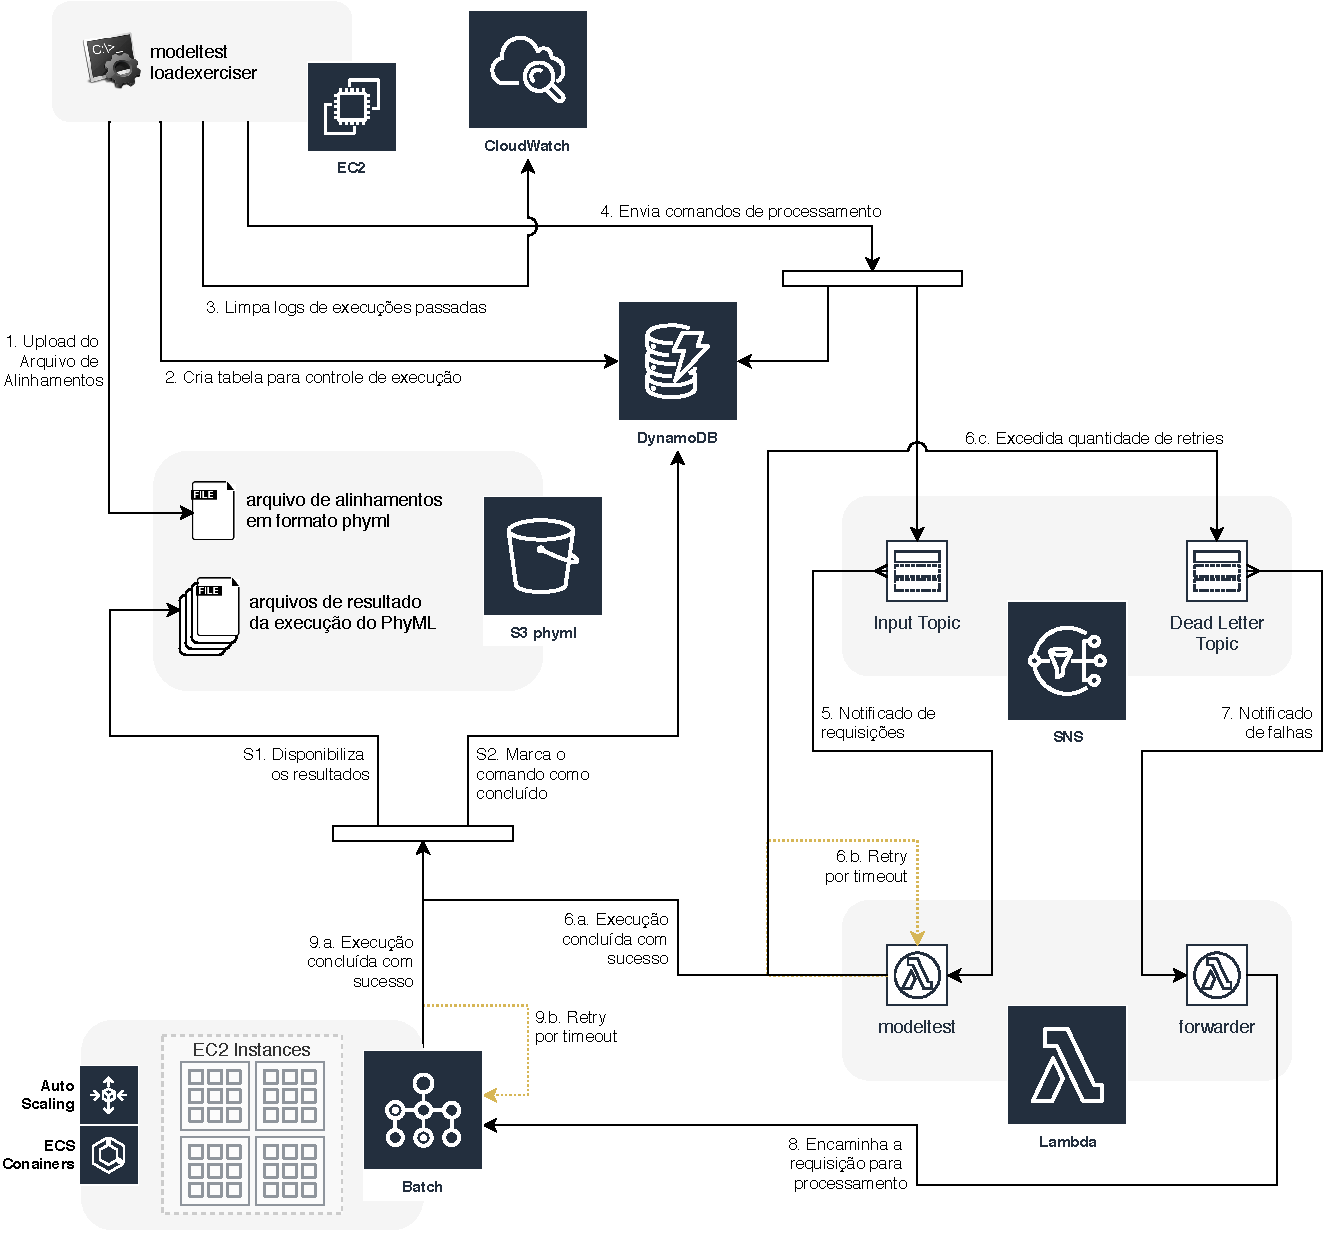
\includegraphics[width=\textwidth]{prototipo-arquitetura}
		\fonte{Elaborado pelo autor.}
	\end{minipage}
\end{figure}


A arquitetura do projeto desenvolvido para o protótipo do modelo \textsf{He}--lastic pode ser vista na \autoref{fig:metodologia-prototipo-arquitetura} que, além dos componentes e suas relações, apresenta também um fluxo de execução para referência.
%
Cabe ressaltar, que o papel das duas camadas de elasticidade está dividido entre os componentes Batch, que assume as funções referentes à camada por Orquestração de Contêineres, e o componente Lambda, mais precisamente através da função \texttt{modeltest} que assume responsabilidade da camada FaaS.
%
Embora não seja evidente na figura, é importante reforçar que a camada FaaS é caracterizada por sua capacidade de escalar rapidamente para atender centenas de requisições, sendo esta propriedade especialmente relevante para a implementação do \texttt{modeltest}.



A ausência de comunicação lateral entre tarefas da aplicação jModelTest e, consequentemente do protótipo, favorece o cenário implementado ao adotar a técnica de comunicação indireta por meio de armazenamento, neste caso o S3, de maneira muito similar a estratégia adotada por \citetexto{Shankar2018}.
%
Os pilares da implementação estão na idempotência, ou seja, a capacidade de aplicar várias vezes a mesma computação e obter sempre o mesmo resultado, independentemente de resultados anteriores e sem efeitos colaterais, 
e na definição de que uma tarefa só será removida do armazenamento de estado, papel desempenhado pelo DynamoDB, depois que sua computação estiver realizada e os resultados disponibilizados.
%
Através destas estratégias, o protótipo não precisa de garantias firmes quanto as capacidades de outros elementos da arquitetura, como por exemplo, as filas de mensagens implementadas pelo SNS, que oferecem apenas garantias \textit{at least once} (pelo menos uma vez), ao invés da garantia mais complexa de \textit{exactly once} (exatamente uma vez), favorecendo a portabilidade e aumentando a confiabilidade do modelo e, por consequência, do protótipo.



Também se tornam aparentes, em função das escolhas arquiteturais, as propriedades de tolerância a falha e recuperação presentes no modelo \textsf{He}--lastic.
%
Assim como em \citetexto{Jonas2017}, a garantia de operações atômicas fornecida pelo armazenamento de estado (DynamoDB) é suficiente para garantir o sucesso de uma execução, embora, para um nível extra de garantias, este desfecho possa ser validado através da checagem dos arquivos de resultado presentes no armazenamento do S3.
%
Desta forma, não há necessidade de gerenciar ou recuperar tarefas que podem ter sido abandonadas durante o processamento, uma vez que é seguro consultar diretamente o armazenamento de estado e de objetos para determinar todas as tarefas não concluídas, reduzindo a complexidade da implementação de tolerância a falhas do modelo \textsf{He}--lastic a um problema de recuperação de tarefas abortadas.
%
Contudo, devido a sua arquitetura em duas camadas, a recuperação pode acontecer por meio de três mecanismos distintos: 
\begin{inparaenum}[\itshape a\upshape)] 
	\item \textit{retry} de tarefas na camada FaaS;
	\item \textit{retry} de tarefas na camada de Orquestração de Contêineres; e
	\item encaminhamento de tarefas falhadas da camada FaaS para a camada de Orquestração de Contêineres.
\end{inparaenum}
Sendo esta última estratégia um dos diferenciais do modelo e do protótipo aqui descritos.



As decisões de arquitetura, tanto do modelo quando do protótipo, favorecem o comportamento independentemente escalável e elástico dos seus componentes, favorecendo não somente a execução de alta performance, como a progressividade nos custos associados a execução de aplicações baseadas no modelo proposto.
%
Esta característica é particularmente relevante em contextos de baixos recursos financeiros ou de pequena escala, que não podem se dar ao luxo de gastar mais do que os já apertados orçamentos.
%
O modelo \textsf{He}--lastic também pode ser uma alternativa viável para instituições maiores e que possuem recursos computacionais.
%
Contudo, conforme afirma \citetexto{Shankar2018}, tais recursos tradicionalmente se mostram de difícil acesso devido às longas filas de esperas por alocação de tempo de computação ou encontram-se impedidos por grandes volumes de processos e burocracias, desencorajando seu uso.






\subsection{Desafios e Dificuldades}
\label{sec:metodologia-prototipo-dificuldades}


Dentre as dificuldades encontradas no desenvolvimento do protótipo, duas delas tem impacto significativo nos resultados e devem ser abordadas.
%
A primeira dificuldade se origina do fato de que, ao contrário de outros projetos científicos e de boa parte dos \textit{benchmarks} sintéticos não há um controle explícito sobre o grão de paralelismo que será computado.
%
Esta ausência de uma unidade de medida para o nível de granularidade exigiu a formalização da \autoref{eq:custo-jmodel-bestfit}, como uma maneira de determinar a granularidade e, assim, incluir no \textit{dataset} de testes, arquivos capazes de representar níveis variados de granularidade computacional, conforme mostra a \autoref{tab:metodologia-etapas-dataset}.


A ausência de controle sobre o número de \textit{retries} executada nas funções Lambda, da camada FaaS, se manifestou como a segunda dificuldade relevante para este trabalho.
%
Visando aumentar a confiabilidade das operações e sendo uma decisão justificável, quando adotado o ponto de vista original a respeito das funções lambda, que objetivam execuções de curta duração orientadas a eventos, o estabelecimento por parte da AWS de um número fixo de 3 \textit{retries} combinado com espera por \textit{backoff} exponencial, tornou-se um problema para o protótipo do modelo \textsf{He}--lastic.
%
Devido à proporcionalidade entre o \textit{timeout} da função e o tempo de \textit{backoff}, a espera em caso de erro injeta um \textit{delay} significativo no processamento, sendo especialmente nocivo em cenários de \textit{timeout} longo e onde parte significativa dos cálculos de adequação de sistemas de evolução não conseguem ser absorvidos pela camada FaaS.
%
O resultado se manifesta como um tempo de espera, onde não é realizada nenhuma computação útil nos cenários em que justamente haveria maior necessidade de agilidade, devido ao alto número de requisições que a camada FaaS (Lambda) não consegue atender e que entrarão na fila para processamento, via elasticidade reativa na camada de Orquestração de Contêineres (Batch).



Devido a ausência de parâmetros para configurar o comportamento de \textit{retry} do Lambda, iniciaram-se esforços em busca de uma solução para contornar este cenário, no entanto, por ser intimamente ligado ao serviço, não foi possível encontrar uma solução capaz de burlar completamente o comportamento de \textit{retry} e o impacto no tempo de execução e no custo que traz consigo.
%
Como estratégia para redução dos tempos de espera foi embutida na função \texttt{\textit{forwarder}} da camada FaaS, a capacidade de disparar ações preparatórias de elasticidade no serviço Batch, representante da camada de Orquestração de Contêineres.
%
Esta forma de heurística usa dados a respeito da fila de execuções do Batch para determinar um número apropriado de vCPUs para requisitar, de forma a evitar a espera pelo \textit{ramp--up} orgânico das ações de elasticidade sem, no entanto, requisitar um número excessivo de recursos, que podem ser rapidamente descartados, o que origina o comportamento de \textit{thrashing}, enquanto respeita os limites superior e inferior, quanto ao número de recursos disponíveis.
%
Desta forma, cada vez que uma nova tarefa que falhou na camada FaaS chega para encaminhamento para a camada de Orquestração de Contêineres, a função \texttt{\textit{forwarder}} avalia a quantidade de tarefas pendentes no Batch (Orquestrador de Contêineres) e, no caso de uma variação significativa entre tarefas pendentes e recursos disponíveis, solicita uma readequação.
%
Esta ação permite burlar o tempo necessário para que as primeiras ações de elasticidade entrem em efeito e comecem a aumentar a quantidade de recursos até o equilíbrio, podendo ser encarada (com a devida licença poética) como \textquoteleft pré--aquecimento do forno\textquoteright, contudo, sem desperdício, uma vez que a ação só é realizada quando há de fato tarefas sendo encaminhadas para o Orquestrador de Contêineres.



Uma evolução desta heurística pode se basear na existência de recursos ativos na camada do Orquestrador de Contêineres e na probabilidade de uma tarefa exceder o tempo limite na camada FaaS, para realizar o \textit{pass--through}, ou seja, encaminhar esta requisição diretamente para o Batch, ao invés de permitir seu processamento pelo Lambda.
%
Uma forma simplificada desta heurística poderia tomar como entrada uma taxa de requisições com falha sobre o total, definindo que, caso a taxa de falha ultrapasse um determinado \textit{threshold}, as demais tarefas serão encaminhadas diretamente para a próxima camada.
%
Embora mais simples, esta versão da heurística corre o risco de obter uma alta taxa de ineficiência quando confrontada com tarefas heterogêneas ou com ampla variação na complexidade, como é o caso da aplicação adotada neste trabalho.
%
Estas estratégias, contudo, poderiam mitigar os problemas com a espera ociosa em função do \textit{retry} de tarefas e impactariam positivamente no custo, evitando repetir três vezes na camada FaaS, uma computação que já está fadada ao fracasso.
%
Entretanto, devido à dificuldade em determinar a probabilidade de uma tarefa exceder o tempo limite na camada FaaS, ou as possíveis deficiências da versão simplificada, estas heurísticas não foram implementadas no protótipo do modelo \textsf{He}--lastic, sendo mantidas como indicação para trabalhos futuros.




\subsection{Parâmetros}


\begin{figure}[b]
	\centering%
	\begin{minipage}{\textwidth}
		\caption{Parâmetros de configuração do protótipo conforme especificados no arquivo serverless.yml e suas equivalências sobre as definições da \autoref{tab:modelo-arq-params}.}
		\label{fig:metodologia-parametros-yaml}
		\vspace{1ex}
		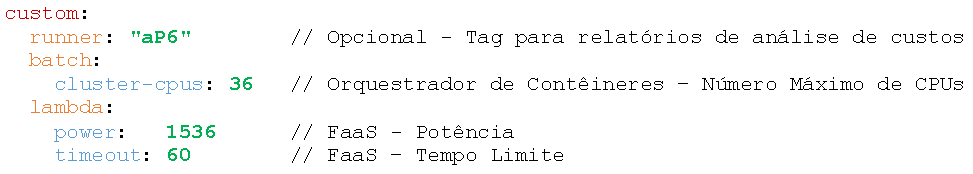
\includegraphics[width=\textwidth]{metodologia-parametros-yaml}
		\fonte{Elaborado pelo autor.}
	\end{minipage}
\end{figure}


Em função das decisões de projeto e arquitetura do protótipo do modelo \textsf{He}--lastic, uma simplificação dos parâmetros do modelo foi possível.
%
Conforme abordado na \autoref{tab:modelo-arq-params}, o modelo \textsf{He}--lastic contempla em seu projeto cinco parâmetros que determinam o comportamento das camadas de elasticidade, sendo, dois deles, a respeito do FaaS e, os demais, sobre a camada de Orquestração de Contêineres.
%
A diferença se dá em função do uso do serviço Batch para gerenciar a camada de Orquestração de Contêineres, onde os \textit{thresholds}, ou seja, os limites que controlam a agressividade do comportamento das ações de elasticidade, são gerenciados de maneira automática e com base na quantidade de itens em espera.


Esta diferença permitiu reduzir de cinco para apenas três os parâmetros do modelo e não foi considerada relevante do ponto de vista de avaliação e testes do modelo \textsf{He}--lastic, haja vista que os cenários de avaliação delineados na \autoref{sec:metodologia-etapas-modelo} não previam variações nos \textit{thresholds} de elasticidade.
%
Embora os parâmetros sejam significativos para uma otimização fina em cenários produtivos em que o modelo seja implementado, o principal objetivo da atual avaliação está em determinar o impacto da estratégia e a interação entre as duas camadas de elasticidade.
%
Desta forma, na relação entre conveniência e controle apresentada pelo uso do AWS Batch contra a gestão manual da camada de Orquestração de Contêineres, por meio dos \textit{thresholds} de elasticidade, foi favorecido o uso do serviço Batch devido à significativa redução no esforço de desenvolvimento e impacto negligenciável na estratégia de avaliação.



Em função da adoção da estratégia de \textit{infrastructure as code}, habilitada através do \textit{serverless framework} e o serviço CloudFormation é possível exercer controle sobre todos os parâmetros do protótipo a partir de um ponto central de configuração presente no arquivo \texttt{serverless.yml}.
%
A \autoref{fig:metodologia-parametros-yaml} apresenta uma amostra do arquivo de configurações, detalhando a definição dos parâmetros de configuração.
%
Desta forma, toda a criação e remoção do ambiente necessário para execução dos cenários de avaliação pode ser realizada com apenas dois comandos fornecidos pelo \textit{serverless framework}, garantindo a reprodutibilidade dos testes e a ausência de artefatos oriundos de execuções anteriores e que poderiam influenciar nos resultados.



\section{Considerações Parciais}


%Este capítulo apresentou a metodologia utilizada para a avaliação do modelo. Foram
%desenvolvidos protótipos tanto da aplicação paralela quanto do Gerenciador AutoElastic utilizando a linguagem Java. O ambiente de testes em que os protótipos foram testados consistem em um ambiente de nuvem OpenNebula. Esta ferramenta oferece uma API Java utilizada pelo Gerenciador para realizar as tarefas de monitoramento e reorganiza- ção de recursos. A aplicação paralela utilizada no ambiente realiza o processamento de uma lista de funções integrais em intervalos determinados. Buscando avaliar o modelo de- senvolvido, foram modeladas diferentes comportamentos de carga de trabalho para serem enviadas para a aplicação computar através de diferentes parametrizações para cada uma das funções a serem calculadas. No que diz respeito à avaliação, foram definidos diferen- tes cenários em que a aplicação será submetida para processamento. A fim de realizar uma comparação direta dos benefícios que a elasticidade pode proporcionar, esses cenário compreendem:


O presente capítulo detalhou os tópicos relacionados a avaliação do modelo proposto, contemplando desde características das etapas e cenários de avaliação, assim como particularidades da aplicação, da infraestrutura de computação em nuvem e detalhes de implementação do protótipo.
%
A respeito do protótipo chamam a atenção características como o amplo uso de serviços de computação em nuvem e a relação entre o Orquestrador de Contêineres e o componente FaaS, o que permitiu amplo reaproveitamento de código.
%
O uso de ferramentas como \textit{docker} e o \textit{serverless framework} permitiram que o protótipo adotasse uma abordagem de infraestrutura como código, onde toda a criação do ambiente necessário para execução é descrita em código--fonte, facilitando a criação e remoção de ambientes e, consequentemente, melhorando a reprodutibilidade dos cenários executados.
%
A arquitetura do protótipo se manteve próxima daquela especificada na proposta do modelo com a notável diferença que o ambiente local, e por consequência a interação com o \textit{software} jModelTest, não foi implementado.


Foram descritas, também, as principais características da infraestrutura de computação em nuvem, abordando questões como serviços utilizados, o conceito de zonas de disponibilidade e precificação empregados pelo provedor AWS.
%
No que diz respeito a aplicação utilizada como referência para o desenvolvimento, o jModelTest, foi abordada, neste capítulo, a íntima relação entre o programa jModelTest e o PhyML, o que permitiu ao protótipo explorar características desta relação para implementar uma abordagem que, ao mesmo tempo que reduz o esforço de desenvolvimento, mantém as mesmas garantias quanto a completude e confiabilidade dos testes realizados, assim como seus resultados.
%
Também foram especificados arquivos contidos no \textit{dataset} de testes assim como os parâmetros de execução e os cenários de avaliação, tanto para o jModelTest, quanto para o modelo proposto, que determinam as características dos cenários de avaliação e serão os insumos das etapas seguintes de limpeza e análise dos dados.







\chapter{Resultados}
\label{ch:resultados}

\epigrafecap{The purpose of life is not to be happy --- but to matter, to be productive, \\ to be useful, to have it make some difference that you have lived at all.}{Leo Rosten}



Neste capítulo são apresentados os resultados obtidos por meio da execução da metodologia de avaliação sobre o \textit{software} jModelTest e o protótipo do modelo \textsf{He}--lastic.
%
Dentre os objetivos deste capítulo é possível citar a compreensão da proporcionalidade de custos entre as camadas de elasticidade do modelo, a caracterização do comportamento do projeto jModelTest, assim como o estudo das características do modelo proposto, seja na sua execução com apenas a camada FaaS, ou somente Orquestrador de Contêineres e, por fim, de ambas as camadas em conjunto.



Como etapa inicial rumo a caracterização dos resultados, uma análise de custo--benefício é realizada utilizando dados artificiais para exercitar diferentes conjuntos de parâmetros possíveis para as camadas de elasticidade do modelo \textsf{He}--lastic.
%
Através destes dados será possível determinar se características como a associatividade de custos se aplica às camadas de elasticidade, assim como prever o impacto nos custos das mudanças nos parâmetros de execução.
%
Esta análise, ainda que realizada com dados simulados, se mostra muito útil para realçar as similaridades e diferenças do modelo proposto frente a outras técnicas computacionais, salientando as propriedades únicas oriundas da combinação entre camadas de elasticidade.



No que tange aos resultados referentes à execução dos cenários de avaliação do jModelTest o objetivo é caracterizar, da maneira mais fiel possível, seu comportamento de escalabilidade assim como os tempos de execução.
%
Através da análise de registros de utilização de CPU, assim como os tempos de execução dos cenários, será possível verificar o grau de eficiência do programa e avaliar as decisões tomadas durante seu desenvolvimento.



Em seguida poderão ser analisados os resultados obtidos através da execução dos cenários de testes do modelo \textsf{He}--lastic, onde poderão ser avaliados de maneira isolada, ou já traçando paralelos com os resultados do jModelTest, obtidos anteriormente.
%
Neste caso a avaliação será dividida em três etapas correspondentes às configurações das camadas de elasticidade, sendo elas: somente FaaS, somente Orquestrador de Contêineres, e camadas combinadas.
%
É de especial interesse uma comparação entre as características da execução com ambas as camadas versus cada camada individualmente, pois assim será possível determinar quais conjuntos de características o modelo proposto herdou de cada camada, sejam elas características positivas ou negativas para as métricas de tempo de execução e custo financeiro.



Por fim serão contrastados os cenários de avaliação especificamente no que diz respeito aos custos financeiros, uma análise que visa determinar qual das abordagens é mais eficaz na utilização de recursos.
%
Também é de grande interesse verificar o impacto que a transição entre camadas das tarefas em execução tem no custo financeiro associado ao cenário de teste.
%
O uso deste tipo de avaliação permite estabelecer uma visão consolidada a respeito das características de performance e custo financeiro, que permite aos usuários do modelo avaliar a viabilidade do uso conforme seus próprios contextos, seja para utilizar o modelo \textsf{He}--lastic ou mesmo manter a utilização do jModelTest.





\section{Estudo de Custo--Benefício}
\label{sec:modelo-custben}

%ABORT: %todo: xupinhar algumas coisas do BBVAServerlessEconomics

\begin{table}[tb]
	\centering%
	\begin{minipage}{\defaultFigureWidth\textwidth}
		\caption{Análise do comportamento das métricas Custo e Financeiro aplicados no modelo de computação FaaS conforme parâmetros requeridos pelo modelo \textsf{He}--lastic.}
		\label{tab:modelo-custben-faas}
		\vspace{1ex}
		%\small
		% qualidative 3-class Pastel2
		\definecolor{c1}{HTML}{b3e2cd}%
		\definecolor{c2}{HTML}{fdcdac}%
		\definecolor{c3}{HTML}{cbd5e8}%
		%
		\begin{tabularx}{\textwidth}{rrrrrWWrr}
			\toprule
			\# & \multicolumn{1}{c}{Memória} & \multicolumn{1}{c}{CPU\textsuperscript{\ddag}} & \multicolumn{1}{c}{\begin{tabular}[c]{@{}c@{}}Tempo\\ Efetivo\end{tabular}} & \multicolumn{1}{c}{\begin{tabular}[c]{@{}c@{}}Tempo\\ Máximo\end{tabular}} & {$y$} & {$t$} & \rotatebox[origin=c]{\tabelaAngulo}{\begin{tabular}[c]{@{}c@{}}$ Custo $ \\[1ex]\end{tabular}} & \rotatebox[origin=c]{\tabelaAngulo}{\begin{tabular}[c]{@{}c@{}}$ Financeiro $ \\[3ex]\end{tabular}} \\ 
			\midrule
			1 & 128 & 8\% &  & 00:11,250 & 2 & 113 & 225 & 0,000023 \\
			2 & 256 & 17\% &  & 00:22,500 & 4 & 225 & 900 & 0,000094 \\
			\rowcolor{c1}
			3 & 384 & 25\% &  & 00:45,000 & 6 & 450 & 2700 & 0,000281 \\
			\rowcolor{c1}
			4 & 768 & 50\% & 00:22,500 & 01:30,000 & 12 & 225 & 2700 & 0,000281 \\
			\rowcolor{c2}
			5 & 768 & 50\% &  & 03:00,000 & 12 & 1800 & 21600 & 0,002251 \\
			6 & 1536 & 100\% &  & 01:00,000 & 24 & 600 & 14400 & 0,001500 \\
			\rowcolor{c2}
			7 & 1536 & 100\% &  & 01:30,000 & 24 & 900 & 21600 & 0,002251 \\
			8 & 1536 & 100\% &  & 03:00,000 & 24 & 1800 & 43200 & 0,004501 \\
			9 & 1920 & 125\% &  & 06:00,000 & 30 & 3600 & 108000 & 0,011253 \\
			\rowcolor{c3}
			10 & 2560 & 170\% &  & 12:00,000 & 40 & 7200 & 288000 & 0,030007 \\
			\rowcolor{c3}
			11 & 3008 & 200\% & 10:12,766 & 15:00,000 & 47 & 6128 & 288000 & 0,030007 \\
			12 & 3008 & 200\% &  & 15:00,000 & 47 & 9000 & 423000 & 0,044073 \\ 
			\bottomrule
		\end{tabularx}
		\tabelafootnote{\textsuperscript{\ddag}~~Se refere à alocação proporcional de CPU onde 200\% equivale à completa alocação de duas vCPUs}
		\tabelafootnote{{*}~Para as demais variáveis das equações de Custo e Financeiro foram adotados os seguintes valores: $ c = y $ e $ m = 1\text{,}04191\text{e-}7 $ }
		\fonte{Elaborado pelo autor.}
	\end{minipage}
\end{table}



A estratégia de dupla camada de elasticidade adotada pelo modelo \textsf{He}--lastic, apoiada na divisão entre tarefas de curta duração (processadas pela camada FaaS através de alto nível de paralelismo) e tarefas de longa duração (processadas pelo Orquestrador de Contêineres), introduz a necessidade de que se estabeleça uma linha de corte que define a fronteira entre ambas camadas.
%
Por meio de uma avaliação preliminar com dados sintéticos é possível verificar a relação entre as camadas de elasticidade, compreendendo em maior profundidade as implicações associadas a cada um dos parâmetros de configuração exigidos pelas camadas FaaS e de Orquestração de Contêineres.
%
Sendo assim, nas próximas subseções são apresentadas as características de precificação de cada uma das camadas de elasticidade, assim como do seu uso misto.





\subsection{Camada FaaS}
\label{sec:modelo-custben-faas}


\begin{figure}[tb]
	\centering%
	\begin{minipage}{\defaultFigureWidth\textwidth}
		\caption[Análise da evolução do custo de execução no modelo de computação FaaS conforme escolhas de parâmetros de Tempo Limite de Execução ($t$) e Memória Alocada ($y$)]{Análise da evolução do custo de execução no modelo de computação FaaS conforme escolhas de parâmetros de Tempo Limite de Execução ($t$) e Memória Alocada ($y$) com a linha Diagonal mostrando, a cada passo, a duplicação de ambas as dimensões ($ t $ e $ y $)}
		\label{fig:modelo-custben-faas}
		\vspace{1ex}
		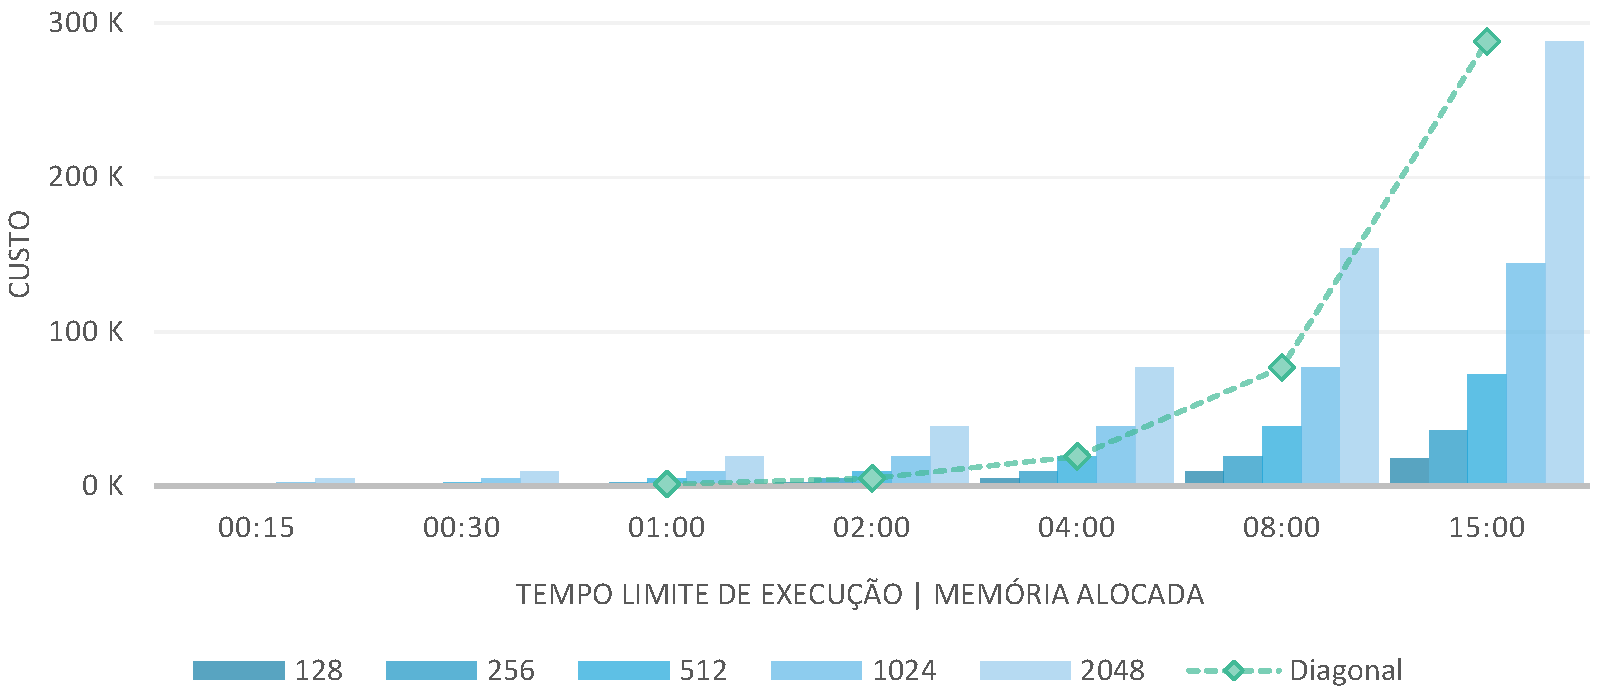
\includegraphics[width=\textwidth]{modelo-custben-faas}
		\fonte{Elaborado pelo autor.}
	\end{minipage}
\end{figure}


Com vistas a um melhor entendimento do funcionamento da camada de curta duração, implementada através de FaaS, e por intermédio das definições prévias a respeito das métricas de avaliação do modelo \textsf{He}--lastic é apresentado, na \autoref{tab:modelo-custben-faas}, um estudo a respeito das escolhas de parâmetros da camada adotando o provedor AWS como referência.
Através dos resultados apresentados neste estudo, é possível notar que a propriedade de associatividade de custos se mantém ao analisar as duplas em destaque referentes aos cenários \{3, 4\}, \{5, 7\} e \{10, 11\}, evidenciando a relação entre o tempo efetivo de execução, o tempo limite de execução e a medida de potência, definida, no estudo da \autoref{tab:modelo-custben-faas}, como a alocação de memória, conforme adotado pela AWS.


Embora o modelo de execução baseado em FaaS evite custos ociosos na ausência de requisições, obsoletando a necessidade de recursos que podem permanecer ociosos por longos períodos de tempo aguardando requisições (com \textit{web--servers} e servidores de banco de dados com baixa utilização figurando como exemplos evidentes), ele, em contrapartida, penaliza operações que ficam em espera como requisições remotas, conexão com bancos de dados ou qualquer operação que demande alto volume de I/O ou tráfego de rede.


Desta forma, lançar mão de FaaS para atuar como \textit{load--balancer}, por exemplo, embora seja atualmente uma tarefa que exige poucos recursos computacionais, se mostra uma péssima ideia ao exacerbar alguns dos pontos negativos do modelo de execução, nomeadamente:
\begin{inparaenum}[\itshape a\upshape)]
	\item espera pelo resultado de terceiros, uma vez que o \textit{load--balancer} apenas encaminha e aguarda resposta de um recurso de \textit{back--end};
	~
	\item alta comunicação de rede, uma vez que o papel de um \textit{load--balancer} é atuar como mediador entre quem faz a requisição e quem efetivamente atende a mesma; e, finalmente
	~
	\item tempo de execução, que causaria requisições perdidas e sem resposta quando excedesse os limites estabelecidos.
\end{inparaenum}
Causando, por fim, uma grande ineficiência ao incorrer custos em um cenário onde há pouca computação e muita espera.


No que diz respeito a memória, considerando dados das Tabelas \ref{tab:FaaS-implementations} e \ref{tab:custo-faas}, as principais implementações de FaaS se apresentam flexíveis o suficiente para uma ampla gama de \textit{workloads}.
Contudo, no que diz respeito a cálculos com grande exigência de memória, os limites estabelecidos inviabilizam seu uso.
Considerando que a razão $ Mem\acute{o}ria~{\small (GB)} \div Cores $ nas FaaS se mantém entre $ 1,5x $ e $ 2x $ nos principais provedores, ela se mostra baixa quando comparada a ofertas de instâncias (VMs) otimizadas para memória, com famílias como as \texttt{x1} e \texttt{r4} da AWS oferecendo, respectivamente, razões de $15,25x$ e $7,625x$.
Situação similar poderia ser observada ao comparar a performance computacional das FaaS contra instâncias otimizadas para processamento, conforme evidência informal publicada por \cite{CloudABC}.
Contudo, tais análises não representam o caso de uso projetado para as FaaS uma vez que ignoraram fatores como a ausência de custos em função de ociosidade, a granularidade da cobrança e a possibilidade de paralelismo massivo.


Entretanto, ainda que a camada FaaS seja usada em cenários favoráveis compostos por alto processamento, alto paralelismo e baixa comunicação, como é o caso no modelo \textsf{He}--lastic, uma característica do seu cálculo de custo, conforme detalhado pela \autoref{eq:custo-faas}, exige cuidados especialmente relevantes para a análise de custo benefício.
O fato de que os parâmetros de memória, CPU e tempo limite, $y$, $c$ e $t$, respectivamente, são multiplicados entre si, faz desta métrica uma unidade composta, tornando o cálculo de $ Custo $ e $ Financeiro $ contra--intuitivo por configurar uma função polinomial de grau três.
O resultado desta característica pode ser observado na \autoref{fig:modelo-custben-faas} indicando uma possível explosão no custo em função da relação entre os parâmetros de memória e tempo limite de execução no cenário, que e simulado adotando o modelo de cobrança do provedor AWS ($ c = y $, conforme \autoref{tab:custo-faas}).



Em casos de uso produtivo das FaaS é esperado que o custo observado seja inferior aos custos apresentados aqui, haja vista de que os estudos realizados adotam os limites máximos como referência, ignorando o fato de que a cobrança se dá por frações de segundos na maioria dos provedores de computação em nuvem.
Ainda assim, para o modelo \textsf{He}--lastic e sua arquitetura baseada em duas camadas de elasticidade, tais estudos representam uma análise relevante em função de que é aceito e esperado que uma parcela das requisições encaminhadas não seja atendida pela camada FaaS em função do tempo limite de execução configurado.
Desta forma, uma análise quanto ao teto de gastos é fundamental para que sejam determinados os parâmetros do modelo ao levar em conta as propriedades do problema onde o modelo \textsf{He}--lastic será implantado, considerando, entre outros, frequência de requisições, grau de heterogeneidade da carga computacional e orçamento disponível.






\subsection{Camada do Orquestrador de Contêineres}


\begin{figure}[tb]
	\centering%
	\begin{minipage}{\defaultFigureWidth\textwidth}
		\caption{Simulação do comportamento da camada de longa duração do modelo \textsf{He}--lastic mostrando a relação entre a quantidade de requisições e a disponibilidade de recursos para processamento.}
		\label{fig:modelo-custben-container}
		%		\vspace{1ex}
		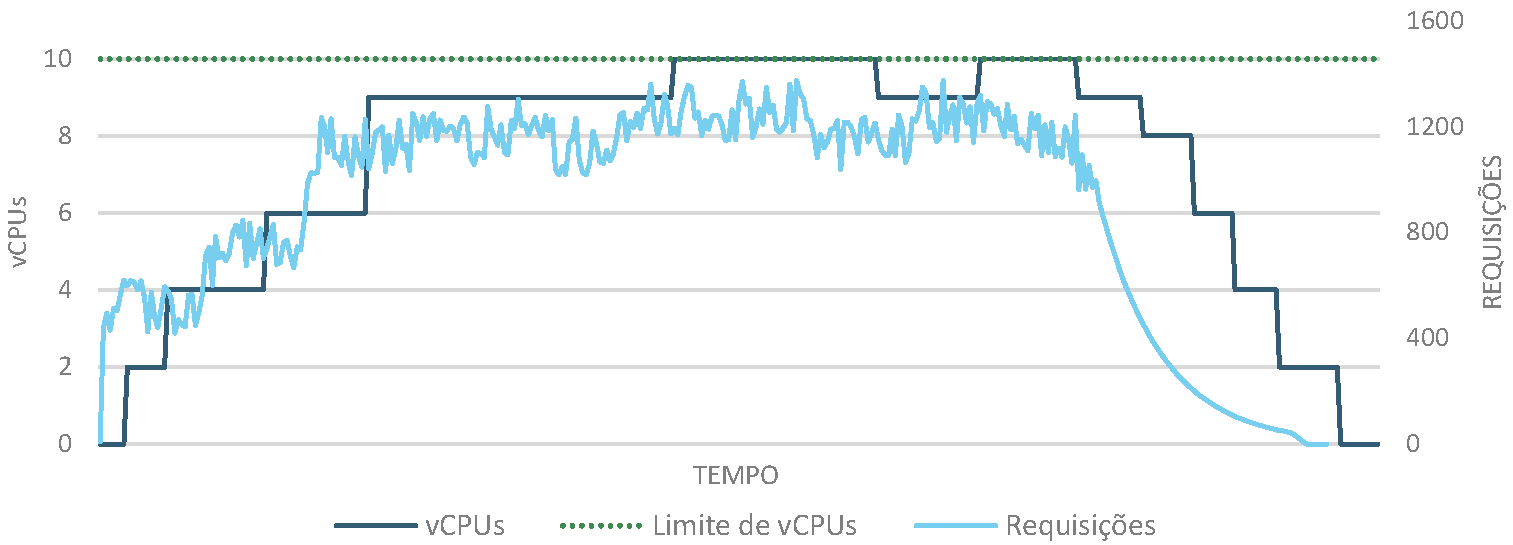
\includegraphics[width=\textwidth]{modelo-custben-container}
		\fonte{Elaborado pelo autor.}
	\end{minipage}
\end{figure}


\begin{table}[tb]
	\centering%
	\begin{minipage}{\defaultFigureWidth\textwidth}
		\caption{Análise do comportamento das métricas Custo e Financeiro aplicados no modelo de computação por Orquestração de Contêineres evidenciando a associatividade de custos.}
		\label{tab:modelo-custben-container}
		\vspace{1ex}
		\centering
		\begin{tabulary}{\textwidth}{rrrrrr}
			\toprule
			\# & Amostras ($ t $) & vCPUs & Custo da Amostra & $ Custo_{elastico} $ & $ Financeiro_{elastico} $ \\ \midrule
			1 & 10 & 16 & 160 & 160 & 6,80 \\
			%			\cmidrule{2-6}
			\dashedline{1-6}
			\multirow{6}{*}{2} & 2 & 2 & 4 & \multirow{6}{*}{160} & \multirow{6}{*}{6,80} \\
			& 2 & 4 & 8 &  &  \\
			& 2 & 8 & 16 & & \\
			& 2 & 16 & 32 &  &  \\
			& 2 & 32 & 64 &  &  \\
			& 2 & 16 & 32 &  &  \\
			& 2 & 2 & 4 &  &  \\
			%			\cmidrule{2-6}
			\dashedline{1-6}
			\multirow{4}{*}{3} & 2 & 16 & 32 & \multirow{4}{*}{160} & \multirow{4}{*}{6,80} \\
			& 2 & 32 & 64 &  &  \\
			& 1 & 48 & 48 &  &  \\
			& 2 & 8 & 16 &  &  \\
			%			\cmidrule{2-6}
			\dashedline{1-6}
			4 & 5 & 32 & 160 & 160 & 6,80 \\
			\bottomrule
		\end{tabulary}
		\tabelafootnote{{*}~Para as demais variáveis das equações de Custo e Financeiro foram adotados os seguintes valores: $ i = 0 $, $ s = 48 $ e $ m = 4\text{,}25\text{e-}2 $ por hora.}
		\fonte{Elaborado pelo autor.}
	\end{minipage}
\end{table}


No que diz respeito ao estudo de custo benefício da segunda camada do modelo \textsf{He}--lastic, previsibilidade e regularidade são fatores primordiais.
Através do uso de \textit{thresholds}, limites superiores e inferiores de carga computacional, o usuário administrador do ambiente de nuvem pode determinar a agressividade com que recursos serão adicionados e removidos.
Ademais, o modelo prevê a existência de um parâmetro que determina a quantidade máxima de CPUs à disposição nesta camada, atuando como limitador de custo.
Através da \autoref{fig:modelo-custben-container} é possível visualizar o comportamento da elasticidade de acordo com a quantidade de requisições e o limite estabelecido para a quantidade de vCPUs disponíveis.
Embora não estejam visíveis na figura, os \textit{thresholds} determinam o quanto o gerenciador de elasticidade vai atuar para manter a ocupação das VMs dentro dos níveis estabelecidos.


A \autoref{tab:modelo-custben-container} apresenta um estudo contemplando quatro cenários em que $ Custo $ e $ Financeiro $ permanecem inalterados mesmo empregando recursos em quantidades variadas.
Embora não seja abordada em detalhes como na camada FaaS, a camada baseada na orquestração de contêineres apresenta os usuais comportamentos de elasticidade, estudados em profundidade em trabalhos como \citetexto{S2016}, \citetexto{Aubin2015}, \citetexto{Coutinho2015}, \citetexto{Righi2013}, \citetexto{Galante2012} e \citetexto{Armbrust:EECS-2009-28}.


Através do uso de um orquestrador de contêineres o modelo \textsf{He}--lastic alivia a carga administrativa e operacional, sendo capaz de delegar a gestão e configuração de máquinas virtuais para o provedor de computação em nuvem e focando seus esforços em preparar somente o \textit{runtime} e o próprio código-fonte da aplicação, resultando, conforme definido nas Decisões de Projeto na \autoref{list:decisoes-de-projeto}, em ganhos de eficiência através da redução do custo total do ambiente, contrastando com um cenário análogo onde fossem utilizados \textit{clusters} ou \textit{grids} computacionais.
Ainda que o tempo de provisionamento de recursos em um cenário de orquestração de contêineres seja similar ao observado quando usadas apenas máquinas virtuais, a vantagem que se obtém é um ambiente de execução agnóstico ao hardware e sistema operacional, evitando a preocupação com os mesmos e permitindo colher os frutos das otimizações realizadas pelos provedores sem a necessidade de reestruturar o código de aplicação.


Diferentemente da camada FaaS, onde não há controle sobre o hardware subjacente, o uso de orquestração de contêineres permite a escolha de famílias de instâncias, dando conta de cenários como os mencionados anteriormente, na \autoref{sec:modelo-custben-faas}, onde existe uma forte demanda por uma única dimensão computacional como memória, CPU e I/O, seja de rede ou armazenamento.
Através desta característica é possível ajustar o modelo \textsf{He}--lastic para que seja capaz de atender a uma ampla gama de cenários, mostrando sua flexibilidade e capacidade de generalização para situações além do cálculo de adequação de sistemas de substituição de sequências moleculares.






\subsection{Camadas Combinadas}


\begin{figure}[tb]
	\centering%
	\begin{minipage}{\defaultFigureWidth\textwidth}
		\caption[Análise de custo por camada para o modelo \textsf{He}--lastic em um cenário de absorção de 50\% das requisições pela camada FaaS]{Análise de custo por camada para o modelo \textsf{He}--lastic em um cenário de absorção de 50\% das requisições pela camada FaaS com base nos dados da \autoref{tab:modelo-custben-misto}.}
		\label{fig:modelo-custben-misto}
		\vspace{1ex}
		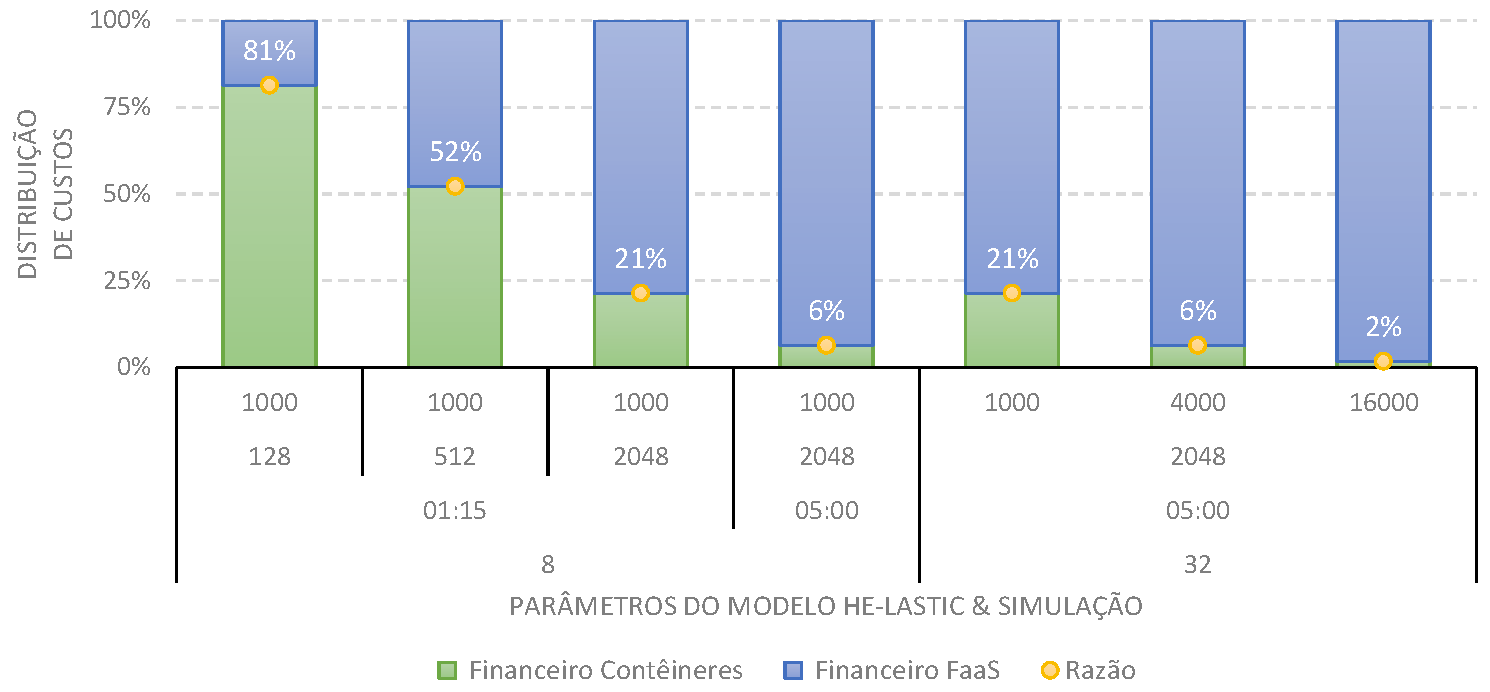
\includegraphics[width=\textwidth]{modelo-custben-misto}
		\fonte{Elaborado pelo autor.}
	\end{minipage}
\end{figure}


\begin{table}
	\centering%
	\begin{minipage}{\textwidth}
		\caption{Análise de custo para o modelo \textsf{He}--lastic ressaltando a relação entre os custos financeiros originados nas camadas FaaS e Orquestrador de Contêineres.}
		\label{tab:modelo-custben-misto}
		\vspace{1ex}
		\footnotesize
		\begin{tabular*}{\textwidth}{@{\extracolsep{\fill}}rrrlrclrrlrrlrc@{}}
			\toprule
			\multicolumn{3}{c}{\begin{tabular}[c]{@{}c@{}}Parâmetros \\ \textsf{He}--lastic\end{tabular}} &\phantom{}&
			\multicolumn{2}{c}{\begin{tabular}[c]{@{}c@{}}Parâmetros \\ da Simulação\end{tabular}} &\phantom{}&
			\multicolumn{2}{c}{FaaS} &\phantom{}&
			\multicolumn{2}{c}{Elástico} &\phantom{}& 
			\multicolumn{2}{c}{Total} \\ 
			\cmidrule(r){1-3}
			\cmidrule(r){5-6}
			\cmidrule(r){8-9}
			\cmidrule(r){11-12}
			\cmidrule(r){14-15}
			\rotatebox[origin=c]{\tabelaAngulo}{vCPUs ($s$)} &
			\rotatebox[origin=c]{\tabelaAngulo}{\begin{tabular}[c]{@{}c@{}}Timeout ($t$)\end{tabular}} & 
			\rotatebox[origin=c]{\tabelaAngulo}{\begin{tabular}[c]{@{}c@{}}Potência ($y$)\end{tabular}} &  &
			\rotatebox[origin=c]{\tabelaAngulo}{\begin{tabular}[c]{@{}c@{}}Requisições\end{tabular}} & 
			\rotatebox[origin=c]{\tabelaAngulo}{\begin{tabular}[c]{@{}c@{}}Absorvidas pela\\ Camada FaaS\end{tabular}} & &
			\begin{tabular}[c]{@{}r@{}}$ Custo $\\ ($\times 10^6$)\end{tabular} & 
			\rotatebox[origin=c]{\tabelaAngulo}{\begin{tabular}[c]{@{}c@{}}$ Financeiro $\end{tabular}} & &
			\rotatebox[origin=c]{\tabelaAngulo}{$ Custo $} & 
			\rotatebox[origin=c]{\tabelaAngulo}{\begin{tabular}[c]{@{}c@{}}$ Financeiro $\end{tabular}} & &
			\rotatebox[origin=c]{\tabelaAngulo}{\begin{tabular}[c]{@{}c@{}}$ Financeiro $\end{tabular}} & 
			\rotatebox[origin=c]{\tabelaAngulo}{Distribuição} \\ 
			\midrule
			\multirow{3}{*}{8} & \multirow{3}{*}{01:15} & \multirow{3}{*}{128} &  & \multirow{3}{*}{1000} & 75\% &  & 1,125 & 0,12 &  & 8 & 0,34 &  & 0,46 & $26:74$ \\
			&  &  &  &  & 50\% &  & 0,75 & 0,08 &  & 8 & 0,34 &  & 0,42 & $19:81$ \\
			&  &  &  &  & 25\% &  & 0,375 & 0,04 &  & 8 & 0,34 &  & 0,38 & $10:90$ \\
			\dashedline{6-15} 
			\multirow{3}{*}{8} & \multirow{3}{*}{01:15} & \multirow{3}{*}{512} &  & \multirow{3}{*}{1000} & 75\% &  & 4,5 & 0,47 &  & 8 & 0,34 &  & 0,81 & $58:42$ \\
			&  &  &  &  & 50\% &  & 3 & 0,31 &  & 8 & 0,34 &  & 0,65 & $48:52$ \\
			&  &  &  &  & 25\% &  & 1,5 & 0,16 &  & 8 & 0,34 &  & 0,50 & $31:69$ \\
			\dashedline{6-15} 
			\multirow{3}{*}{8} & \multirow{3}{*}{01:15} & \multirow{3}{*}{2048} &  & \multirow{3}{*}{1000} & 75\% &  & 18 & 1,88 &  & 8 & 0,34 &  & 2,22 & $85:15$ \\
			&  &  &  &  & 50\% &  & 12 & 1,25 &  & 8 & 0,34 &  & 1,59 & $79:21$ \\
			&  &  &  &  & 25\% &  & 6 & 0,63 &  & 8 & 0,34 &  & 0,97 & $65:35$ \\
			\dashedline{6-15} 
			\multirow{3}{*}{8} & \multirow{3}{*}{05:00} & \multirow{3}{*}{2048} &  & \multirow{3}{*}{1000} & 75\% &  & 72 & 7,50 &  & 8 & 0,34 &  & 7,84 & $96:04$ \\
			&  &  &  &  & 50\% &  & 48 & 5,00 &  & 8 & 0,34 &  & 5,34 & $94:06$ \\
			&  &  &  &  & 25\% &  & 24 & 2,50 &  & 8 & 0,34 &  & 2,84 & $88:12$\rlap{\textsuperscript{\dag}} \\
			\dashedline{6-15} 
			\multirow{3}{*}{32} & \multirow{3}{*}{05:00} & \multirow{3}{*}{2048} &  & \multirow{3}{*}{1000} & 75\% &  & 72 & 7,50 &  & 32 & 1,36 &  & 8,86 & $85:15$ \\
			&  &  &  &  & 50\% &  & 48 & 5,00 &  & 32 & 1,36 &  & 6,36 & $79:21$ \\
			&  &  &  &  & 25\% &  & 24 & 2,50 &  & 32 & 1,36 &  & 3,86 & $65:35$\rlap{\textsuperscript{\dag}} \\
			\dashedline{6-15} 
			\multirow{3}{*}{32} & \multirow{3}{*}{05:00} & \multirow{3}{*}{2048} &  & \multirow{3}{*}{4000} & 75\% &  & 288 & 30,01 &  & 32 & 1,36 &  & 31,37 & $96:04$ \\
			&  &  &  &  & 50\% &  & 192 & 20,00 &  & 32 & 1,36 &  & 21,36 & $94:06$ \\
			&  &  &  &  & 25\% &  & 96 & 10,00 &  & 32 & 1,36 &  & 11,36 & $88:12$ \\
			\dashedline{6-15} 
			\multirow{3}{*}{32} & \multirow{3}{*}{05:00} & \multirow{3}{*}{2048} &  & \multirow{3}{*}{16000} & 75\% &  & 1152 & 120,03 &  & 32 & 1,36 &  & 121,39 & $99:01$ \\
			&  &  &  &  & 50\% &  & 768 & 80,02 &  & 32 & 1,36 &  & 81,38 & $98:02$ \\
			&  &  &  &  & 25\% &  & 384 & 40,01 &  & 32 & 1,36 &  & 41,37 & $97:03$ \\
			\bottomrule
		\end{tabular*}
		\tabelafootnote{{*}~Para as demais variáveis das equações de Custo e Financeiro foram adotados os seguintes valores: 
			FaaS = \{ $ c = y $, $ m = 1\text{,}04191\text{e-}7 $ \} e 
			Elástico \{ $ i = 0$, $t = 1$h, $ m = 4\text{,}25\text{e-}2 $ \}
		}
		\fonte{Elaborado pelo autor.}
	\end{minipage}
\end{table}


Uma vez que o cerne do modelo \textsf{He}--lastic está no uso de suas duas camadas de elasticidade, uma análise prévia de custos se apresenta como uma ferramenta de grande relevância para a definição dos parâmetros do modelo, conforme estabelecidos pela \autoref{tab:modelo-arq-params}.
Contudo, dada a dificuldade em determinar de antemão o tempo efetivo de execução de uma chamada na camada FaaS, assim como, a dificuldade em estimar o impacto dos \textit{thresholds} na elasticidade da camada de Contêineres sem o profundo conhecimento do problema em mãos, ou mesmo um conjunto de resultados experimentais, a análise de custo benefício pode ser realizada por meio de cenários pessimistas, adotando os limites máximos como referência.


A decisão por uma abordagem pessimista favorece a análise de custo benefício ao reduzir para apenas três o número de parâmetros contemplados, sendo eles: 
\begin{inparaenum}[(i)]
	\item Tempo Limite da camada FaaS;
	\item Potência da camada FaaS; e
	\item Número de CPUs do Orquestrador de Contêineres.
\end{inparaenum}
Os dados contidos na \autoref{tab:modelo-custben-misto} são o resultado da análise de custo benefício por camada do modelo \textsf{He}--lastic ao variar os parâmetros do modelo e da simulação de carga.
Através destes resultados é possível visualizar um crescimento não linear nos custos associados à camada FaaS no cenário onde há o aumento no número de vCPUs de 8 para 32 (marcado na tabela com o símbolo \dag), causando, em situação de carga simulada para a camada FaaS de 25\%.
Embora o esperado para esta situação seja um aumento de $4x$ no custo relacionado ao upgrade de 8 para 32 vCPUs, os dados observados são da ordem de $2\text{,}9x$, com a distribuição de custo saindo de $88:12$ para $65:35$.
Tal comportamento é suportado pela análise de custo realizada na \autoref{sec:modelo-custben-faas} e pode ser visualizada tanto nos dados da \autoref{tab:modelo-custben-faas}, quanto no gráfico da \autoref{fig:modelo-custben-faas}.



De maneira a facilitar a visualização deste comportamento, a \autoref{fig:modelo-custben-misto} apresenta um panorama sobre os dados oriundos da \autoref{tab:modelo-custben-misto}, quando limitados ao cenário que contempla uma divisão equalitária entre o atendimento das requisições disparadas.
Ao analisar o gráfico, fica evidente a estreita relação entre o custo da camada FaaS e a quantidade de requisições, uma situação que não se repete na camada baseada em Orquestração de Contêineres, uma vez que seu modelo de custo considera apenas o tempo de uso dos recursos.
Embora não exista, na precificação, a relação entre requisições e tempo de uso, este é um fator relevante na construção dos cenários de análise de custo benefício do modelo \textsf{He}--lastic, visto que, requisições que consomem muitos recursos causarão um aumento no tempo necessário para seu processamento e resultando em um ajuste na variável $t$ do componente $Custo_{elastico}$, conforme apresentado na \autoref{eq:custo-elastico}.
A situação inversa também é relevante para análise pois mostra que o custo oriundo do Orquestrador de Contêineres pode dominar o custo total em cenários de baixo volume de curtas requisições, o que pode resultar em baixa utilização dos recursos disponíveis alocados por esta camada em função da ociosidade.


Contudo, um dos diferenciais do modelo \textsf{He}--lastic se mostra difícil de mapear apenas através de análises de custo em situações de carga.
Devido a forma como as duas camadas de elasticidade são projetadas, uma das propriedades do modelo proposto é sua capacidade de manter custo zero em períodos de ociosidade, diferentemente de abordagens anteriores.
A existência de uma camada de elasticidade baseada em FaaS fornece os mecanismos necessários para ativar, sob demanda, a segunda camada baseada em Orquestração de Contêineres, de forma que, através da combinação de camadas, torna-se possível manter inativa também a segunda camada, contudo livre do risco de rejeitar requisições por falta de servidores.


Outra característica habilitada pela abordagem em duas camadas do modelo \textsf{He}--lastic, é a capacidade de disponibilizar um grande número de recursos computacionais de maneira quase instantânea através da camada FaaS, evitando uma das fraquezas de abordagens baseadas puramente em elasticidade onde é característico um comportamento de \textit{ramp--up}, ou seja, uma crescente na quantidade de recursos disponibilizados até que se obtenha uma situação de equilíbrio.
Com a ajuda da camada FaaS este comportamento é atenuado em casos onde uma parcela das requisições pode ser atendida pela camada FaaS, deixando tempo hábil para que o Orquestrador de Contêineres tenha o tempo necessário para disponibilizar seus recursos.


Tanto a capacidade de manter custo zero, quanto a alteração no perfil de disponibilização de recursos, podem ser vistas na \autoref{fig:modelo-custben-alternativas} que utiliza um cenário simulado para ilustrar as características do modelo.
A situação retratada se estende por um período de um dia, ou seja, 24 horas e contempla dois momentos onde são geradas requisições, respectivamente nas horas 3 e 13.
Em uma situação de recursos fixos, como um servidor dedicado ou até mesmo um \textit{cluster} computacional, são observados períodos significativos de ociosidade até que se configure a utilização total de seus recursos, causando grande desperdício relativo ao período ocioso.
Em um cenário de elasticidade existe uma grande melhora no aproveitamento de recursos devido à capacidade de reduzir o número de processadores ativos enquanto não há trabalho a ser feito.
Contudo, neste modelo de operação ainda não é possível zerar completamente a quantidade de recursos devido a ausência de gatilhos que permitam inicializar operações de elasticidade.
Além disso, há o comportamento característico da elasticidade reativa baseada em \textit{thresholds}, onde a quantidade de recursos deve progressivamente se ajustar às características da demanda, resultando em uma ascendente no consumo de recursos durante as primeiras amostras e, em alguns cenários, uma descendente ao final do processamento.


\begin{figure}[tb]
	\centering%
	\begin{minipage}{\defaultFigureWidth\textwidth}
		\caption{Comportamento esperado sobre o uso de recursos ao longo do tempo conforme modelos de execução baseado em recursos fixos, elasticidade e \textsf{He}--lastic, evidenciando as diferenças no que diz respeito à capacidade ociosa e a evolução no aproveitamento de recursos ao longo do tempo.}
		\label{fig:modelo-custben-alternativas}
		%		\vspace{1ex}
		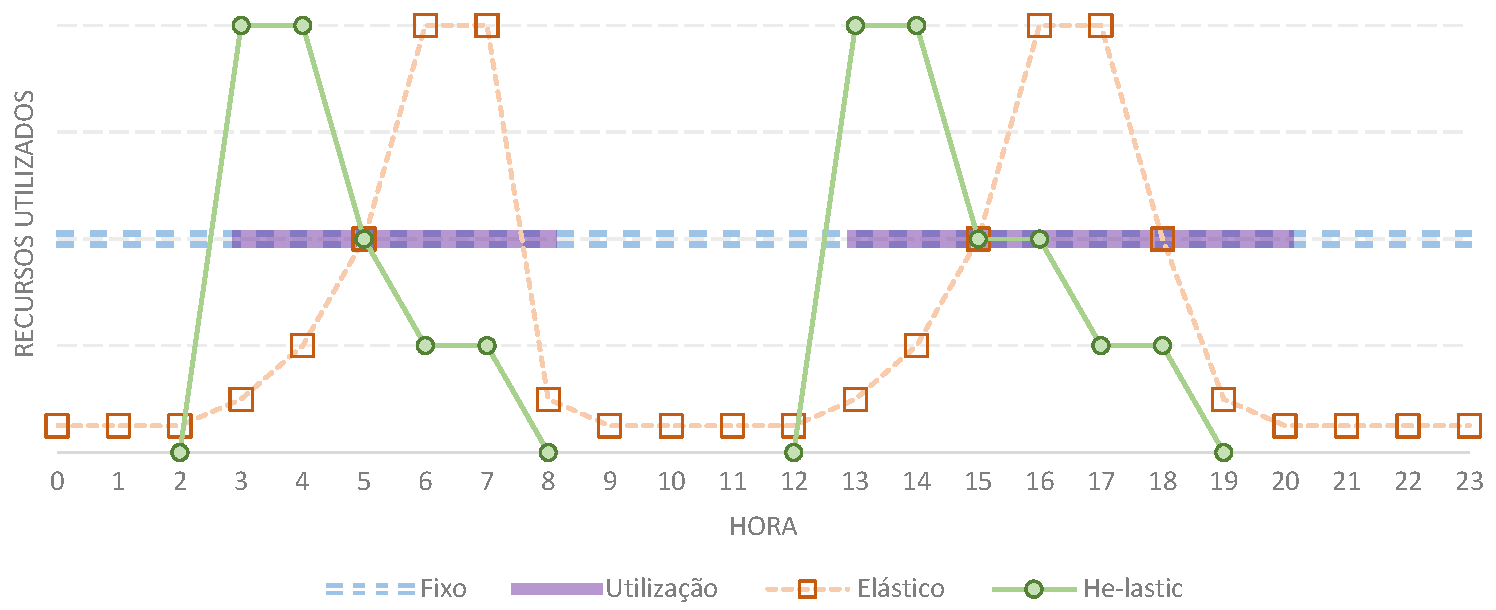
\includegraphics[width=\textwidth]{modelo-custben-alternativas}
		\fonte{Elaborado pelo autor.}
	\end{minipage}
\end{figure}


Por meio dos dados apresentados até aqui é possível concluir que a análise de custo benefício do modelo \textsf{He}--lastic é capaz de estabelecer apenas os limites superiores no que diz respeito ao consumo de recursos e, portanto, o custo financeiro que decorre da execução do modelo com um determinado conjunto de parâmetros.
Embora forneça uma orientação relevante sobre como devem ser definidos os parâmetros do modelo, tal análise permanece insuficiente para a completa determinação de seus valores conforme apresentados na \autoref{tab:modelo-arq-params}.
Este posicionamento se justifica por fatores como a cobrança por tempo efetivo de execução oriunda da camada FaaS e a dependência de dados específicos da aplicação em execução para a determinação da capacidade em termos de requisições por hora, por exemplo, da camada baseada em Orquestração de Contêineres.


Conclui-se, portanto, que a análise de custo benefício e, por consequência, a escolha dos parâmetros de execução para o modelo \textsf{He}--lastic requer insumos oriundos do problema sobre o qual está sendo aplicado, tornando-se uma tarefa de natureza empírica.
Esta conclusão obtém apoio do artigo elaborado pelo banco espanhol de investimentos \textit{Banco Bilbao Vizcaya Argentaria} (BBVA) que, em sua análise do modelo \textit{Serverless} de computação, publicado em \citetexto{BBVAServerlessEconomics}, constrói toda sua análise de custo com a ajuda de uma variável denominada \textquoteleft fator de \textit{throughput}\textquoteright  da aplicação. 
Ainda assim, prova-se, mediante os estudos realizados aqui, que é possível estabelecer o caráter de custo para um conjunto de parâmetros, determinando os limites superiores no que tange ao custo financeiro oriundo da execução do modelo e, portanto, servindo como uma base formal que auxilia nesta tarefa.

%\newpage
%
%Tal estratégia possibilita ao modelo \textsf{He}--lastic atender a uma vasta gama de aplicações através do alto nível de paralelismo na camada FaaS combinado com a flexibilidade da elasticidade tradicional otimizada pelo uso de contêineres.










\section{Avaliação do jModelTest}
\label{sec:resultados-jmodel}


\begin{table}[tbp]
\centering%
\begin{minipage}{\defaultFigureWidth\textwidth}
	\caption{Quantidade de amostras coletadas na avaliação do jModelTest para cada arquivo do \textit{dataset} conforme o cenário.}
	\label{tab:results-jmodel-samples}
	\vspace{1ex}
	\small
	\begin{tabularx}{\textwidth}{lWWWWWW}
		\toprule
		\multicolumn{1}{c}{\multirow{2}{*}{Arquivo}} & \multicolumn{5}{c}{Cenário / vCPUs} & \multicolumn{1}{c}{\multirow{2}{*}{Total}} \\ \cmidrule(lr){2-6}
		\multicolumn{1}{c}{} & $C_{j2}$ & $C_{j4}$ & $C_{j8}$ & $C_{j16}$ & $C_{j36}$ & \multicolumn{1}{c}{} \\ \midrule
		01-aP6 & 19 & 23 & 24 & 11 & 11 & 88 \\
		02-rodents & 20 & 23 & 17 & 11 & 11 & 82 \\
		03-example & 20 & 23 & 16 & 11 & 11 & 81 \\
		04-18S\_insects2 & 20 & 23 & 22 & 11 & 11 & 87 \\
		05-HIVpol.groupM & 20 & 23 & 17 & 11 & 11 & 82 \\
		06-Hex\_EF1a & 20 & 23 & 17 & 11 & 11 & 82 \\
		07-primate-mtDNA & 20 & 23 & 17 & 11 & 11 & 82 \\
		08-HIV\_vpu.ref2 & 20 & 23 & 19 & 11 & 11 & 84 \\
		09-gusanos16S.mafft & 20 & 23 & 18 & 11 & 11 & 83 \\
		10-Birds & 20 & 23 & 17 & 11 & 11 & 82 \\
		11-gusanosCOI.mafft & 20 & 23 & 18 & 11 & 11 & 83 \\
		12-stamatakis-59 & 11 & 19 & 17 & 10 & 10 & 67 \\
		\bottomrule
		\multicolumn{1}{r}{Total} & 230 & 272 & 219 & 131 & 131 & {\footnotesize 983} \\
	\end{tabularx}
	\fonte{Elaborado pelo autor.}
\end{minipage}
\end{table}


\begin{table}[tbp]
\centering%
\begin{minipage}{\defaultFigureWidth\textwidth}
	\caption{Coeficiente de Variação (CV) na avaliação do jModelTest contemplando tempos de execução obtidos por arquivo e cenário de avaliação.}
	\label{tab:results-jmodel-cv}
	\vspace{1ex}
	\small
	\begin{tabularx}{\textwidth}{lWWWWW}
		\toprule
		\multicolumn{1}{c}{\multirow[b]{2}{*}{Arquivo}} & \multicolumn{5}{c}{Cenário / vCPUs} \\ 
		\cmidrule(l){2-6} 
		\multicolumn{1}{c}{} & $C_{j2}$ & $C_{j4}$ & $C_{j8}$ & $C_{j16}$ & $C_{j36}$ \\ 
		\midrule
		01-aP6 & 2\% & 8\% & 18\% & 10\% & 23\% \\
		02-rodents & 1\% & 2\% & 10\% & 0\% & 7\% \\
		03-example & 1\% & 2\% & 10\% & 6\% & 5\% \\
		04-18S\_insects2 & 0\% & 2\% & 14\% & 5\% & 5\% \\
		05-HIVpol.groupM & 0\% & 1\% & 8\% & 1\% & 1\% \\
		06-Hex\_EF1a & 0\% & 1\% & 8\% & 1\% & 2\% \\
		07-primate-mtDNA & 0\% & 1\% & 8\% & 1\% & 1\% \\
		08-HIV\_vpu.ref2 & 0\% & 1\% & 9\% & 1\% & 1\% \\
		09-gusanos16S.mafft & 0\% & 1\% & 8\% & 0\% & 1\% \\
		10-Birds & 1\% & 1\% & 9\% & 0\% & 1\% \\
		11-gusanosCOI.mafft & 0\% & 1\% & 10\% & 0\% & 1\% \\
		12-stamatakis-59 & 1\% & 1\% & 8\% & 0\% & 0\% \\ 
		\bottomrule
	\end{tabularx}
	\fonte{Elaborado pelo autor.}
\end{minipage}
\end{table}


Visando obter resultados de alta confiabilidade, uma vez que estes formariam a régua sobre a qual se apoiam as medidas do modelo proposto, foram realizadas no total quase mil execuções dos testes de adequação de sistemas de substituição molecular seguindo os arquivos, parâmetros e cenários definidos na \autoref{sec:metodologia-etapasecenarios}.
%
Estas execuções foram distribuídas em quase cem (96) máquinas virtuais distintas contemplando instâncias do serviço EC2 da AWS nos seguintes modelos: \texttt{c4.2xlarge}, \texttt{c5.large}, \texttt{c5.xlarge}, \texttt{c5.2xlarge}, \texttt{c5.4xlarge}, \texttt{c5.9xlarge}.
%
Os dados contidos na \autoref{tab:results-jmodel-samples} apresentam os resultados da coleta de dados baseada na execução do jModelTest, totalizando, após filtragem de anomalias (\textit{outliers}), 983 execuções por arquivo--cenário.
%
Para obter a quantidade de chamadas à ferramenta PhyML basta multiplicar os dados da \autoref{tab:results-jmodel-samples} pela \autoref{tab:metodologia-etapas-dataset}, mais especificamente a quantidade de sistemas de substituição molecular contemplados por arquivo quando é seguida a estratégia de \textit{Clustering Search}, resultando em aproximadamente 250 mil (249.184) execuções por arquivo--sistema--cenário.


A respeito da quantidade de amostras cabe ressaltar que a variação no número de coletas do cenário $C_{j8}$ se deu em função de uma limitação do provedor AWS onde inicialmente a conta de usuário utilizada para os testes não tinha acesso à recursos computacionais da família \texttt{c5}, de última geração, de forma que, na época, a estratégia adotada foi prosseguir com os testes utilizando recursos da família \texttt{c4}, da geração anterior.
%
O impacto destas restrições estabelecidas pelo provedor AWS também se manifesta na pequena redução da quantidade de execuções para o arquivo 12-stamatakis-59 que alocava todas as VMs disponíveis por longos períodos de tempo, principalmente nos cenários com menos recursos como $C_{j2}$ e $C_{j4}$, afetando a execução dos demais cenários.
%
Após contato com o provedor foi esclarecido que a ausência destes recursos era um mecanismo de proteção contra abusos visto que tratava-se de uma conta recém aberta.
%
Uma vez detalhados os objetivos da requisição e o contexto de uso, os recursos \texttt{c5} foram liberados e o limite ampliando, possibilitando dar seguimento às avaliações dos cenários.



Contudo, ao detectar uma variação atípica nos tempos de execução, que se manifesta no desvio padrão e no coeficiente de variação (CV\footnote{
	Coeficiente de Variação é uma métrica estatística amplamente utilizada para indicar a precisão, repetitividade e reprodutibilidade de avaliações, atuando também como indicador de dispersão de uma distribuição por incorporar em seu cálculo a média e o desvio padrão, sendo definido pela fórmula:
	\[ \text{CV} = \dfrac{desvio~padr\tilde{a}o}{m\acute{e}dia} \]
}) das amostras coletadas, conforme evidências da \autoref{tab:results-jmodel-cv}, 
foi decidido por aumentar o número de execuções até obter uma variação em linha com os demais cenários e arquivos.
%
Outro padrão que emerge da análise do coeficiente de variação por arquivo e cenário é o alto nível de oscilação apresentado pelo arquivo 01-aP6.
%
Este comportamento está relacionado à sua curta duração e se estende para outros arquivos conforme aumenta a quantidade de recursos disponível, como mostra, por exemplo, o CV de 5\% para o arquivo 04 no cenário $C_{j36}$.
%
Através da análise da \autoref{tab:results-jmodel-cv}, desconsiderando-se o cenário $C_{j8}$ pelos motivos previamente citados, é possível vislumbrar uma 
%TOD0: aplicar cores pra demarcar esta diagonal
diagonal imaginária que abrange os dados de arquivo e cenário: \{03--$C_{j2}$, 04--$C_{j4}$, 04--$C_{j16}$, 06--$C_{j36}$\}.


\afterpage{
	\clearpage
	\begin{landscape}
		\begin{table}
			%\centering%
			\begin{minipage}{\linewidth}
				\caption{Média e Mediana dos tempos de execução observados no jModelTest por arquivo e cenário de avaliação.}
				\label{tab:results-jmodel-avgs}
				\vspace{0.75ex}
				%\small
				\renewcommand\arraystretch{1.35}
				\begin{tabular*}{\linewidth}{@{\extracolsep{\fill}}lrrcrrcrrcrrcrr@{}}
					\toprule
					\multicolumn{1}{c}{\multirow[b]{3}{*}{Arquivo}} & \multicolumn{14}{c}{Cenário / vCPUs} \\ \cmidrule(l){2-15} 
					& \multicolumn{2}{c}{$C_{j2}$} &  & \multicolumn{2}{c}{$C_{j4}$} &  & \multicolumn{2}{c}{$C_{j8}$} &  & \multicolumn{2}{c}{$C_{j16}$} &  & \multicolumn{2}{c}{$C_{j36}$} \\ 
					\cmidrule(lr){2-3} \cmidrule(lr){5-6} \cmidrule(lr){8-9} \cmidrule(lr){11-12} \cmidrule(l){14-15} 
					& \multicolumn{1}{c}{Média} & \multicolumn{1}{c}{Mediana} &  & \multicolumn{1}{c}{Média} & \multicolumn{1}{c}{Mediana} &  & \multicolumn{1}{c}{Média} & \multicolumn{1}{c}{Mediana} &  & \multicolumn{1}{c}{Média} & \multicolumn{1}{c}{Mediana} &  & \multicolumn{1}{c}{Média} & \multicolumn{1}{c}{Mediana} \\ 
					\midrule
					01-aP6 & 0:00:40 & 0:00:40 &  & 0:00:20 & 0:00:21 &  & 0:00:11 & 0:00:11 &  & 0:00:06 & 0:00:06 &  & 0:00:04 & 0:00:04 \\
					02-rodents & 0:03:19 & 0:03:20 &  & 0:01:40 & 0:01:41 &  & 0:00:54 & 0:00:57 &  & 0:00:29 & 0:00:29 &  & 0:00:17 & 0:00:17 \\
					03-example & 0:04:41 & 0:04:42 &  & 0:02:22 & 0:02:23 &  & 0:01:19 & 0:01:22 &  & 0:00:44 & 0:00:45 &  & 0:00:26 & 0:00:27 \\
					04-18S\_insects2 & 0:04:51 & 0:04:52 &  & 0:02:26 & 0:02:27 &  & 0:01:18 & 0:01:23 &  & 0:00:40 & 0:00:41 &  & 0:00:22 & 0:00:22 \\
					05-HIVpol.groupM & 0:11:58 & 0:11:58 &  & 0:06:09 & 0:06:10 &  & 0:03:22 & 0:03:34 &  & 0:01:55 & 0:01:55 &  & 0:01:11 & 0:01:11 \\
					06-Hex\_EF1a & 0:20:11 & 0:20:12 &  & 0:10:14 & 0:10:16 &  & 0:05:27 & 0:05:45 &  & 0:03:05 & 0:03:05 &  & 0:01:45 & 0:01:44 \\
					07-primate-mtDNA & 0:24:22 & 0:24:23 &  & 0:12:25 & 0:12:26 &  & 0:06:45 & 0:07:07 &  & 0:04:00 & 0:04:01 &  & 0:02:37 & 0:02:37 \\
					08-HIV\_vpu.ref2 & 0:45:39 & 0:45:38 &  & 0:22:52 & 0:22:56 &  & 0:11:58 & 0:12:39 &  & 0:06:40 & 0:06:41 &  & 0:03:52 & 0:03:52 \\
					09-gusanos16S.mafft & 1:44:53 & 1:44:52 &  & 0:52:49 & 0:53:06 &  & 0:28:08 & 0:29:46 &  & 0:15:46 & 0:15:47 &  & 0:10:24 & 0:10:24 \\
					10-Birds & 2:11:57 & 2:11:50 &  & 1:07:22 & 1:07:34 &  & 0:36:00 & 0:37:38 &  & 0:20:53 & 0:20:53 &  & 0:12:27 & 0:12:28 \\
					11-gusanosCOI.mafft & 2:58:59 & 2:58:49 &  & 1:30:39 & 1:31:03 &  & 0:47:51 & 0:50:14 &  & 0:27:21 & 0:27:22 &  & 0:16:15 & 0:16:15 \\
					12-stamatakis-59 & 14:52:32 & 14:51:54 &  & 7:28:55 & 7:30:39 &  & 4:02:50 & 4:15:20 &  & 2:19:25 & 2:19:30 &  & 1:23:40 & 1:23:34 \\
					\bottomrule
				\end{tabular*}
				\tabelafootnote{{*}~Valores apresentados em formato hh:mm:ss.}
				\fonte{Elaborado pelo autor.}
			\end{minipage}
		\end{table}
		
		\begin{figure}[bt]
			\centering%
			\begin{minipage}{\linewidth}
				\caption{Representação gráfica da \autoref{tab:results-jmodel-avgs} mostrando os tempos de execução por arquivo e cenário conforme a mediana.}
				\label{fig:results-jmodel-avgs}
				\vspace{1ex}
				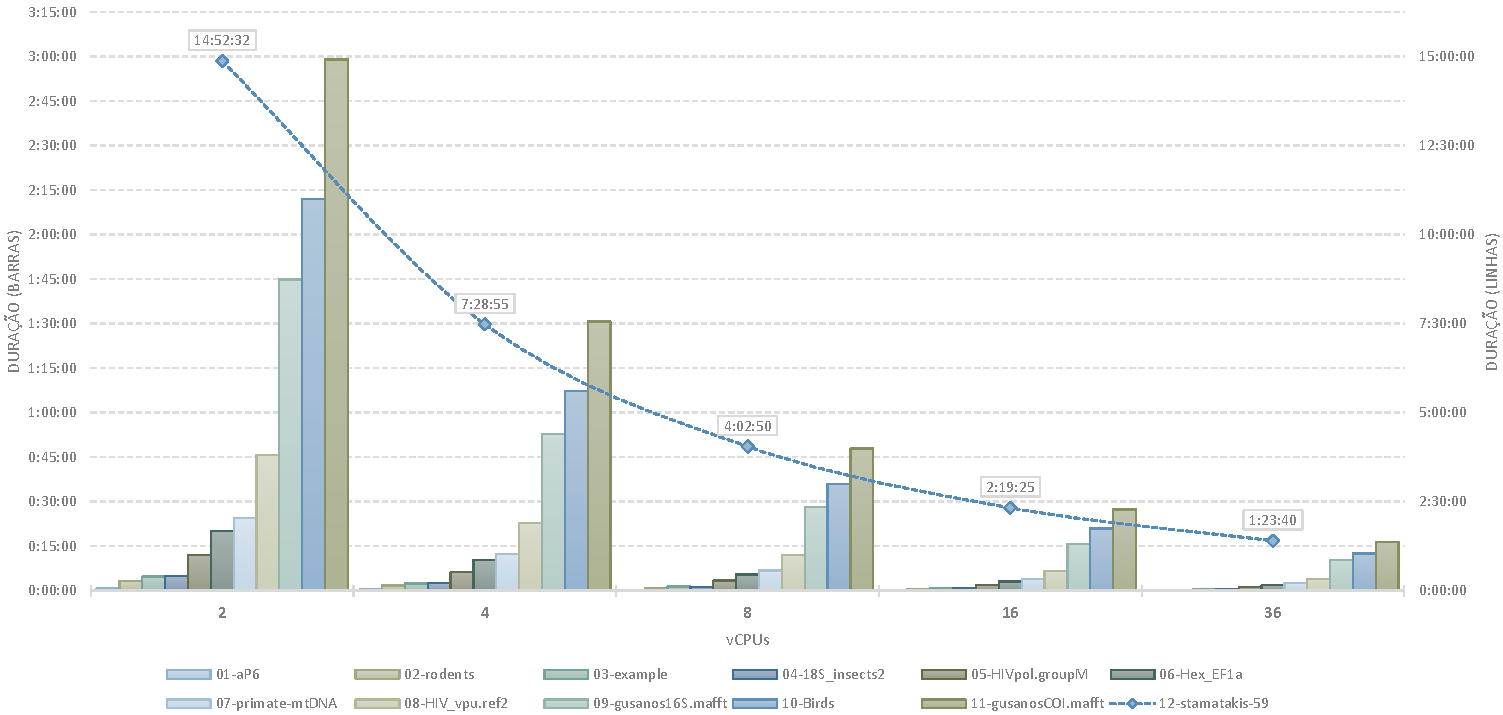
\includegraphics[width=\linewidth]{results-jmodel-avgs}
				\fonte{Elaborado pelo autor.}
			\end{minipage}
		\end{figure}
		
	\end{landscape}
}


Dentre as razões que motivam a alta variabilidade nos tempos de execução é possível citar a curta duração absoluta, medida em termos do tempo total de execução e que pode ser observada na \autoref{tab:results-jmodel-avgs} onde são detalhadas as métricas de média e mediana dos tempos de execução para cada tupla de arquivo e cenário de avaliação.
%
Além de amplificar as diferenças relativas, medida em termos do CV, as tarefas de curta duração são especialmente sensíveis a interferências e/ou irregularidades no processamento que podem originar de uma série de fatores como: política de \textit{scheduling} de processos e \textit{threads}, consumo dos demais processos em execução, I/O de rede e disco, além de fatores típicos de uma ambiente de nuvem como o impacto do virtualizador e o efeito popularmente conhecido como \textit{noisy neighbor} em que os processos em execução por outro \textit{tenant}, que divide o mesmo recurso físico, podem afetar a performance das demais VMs.


Entretanto é possível afirmar que as métricas de média e mediana encontram-se, de maneira geral, bastante alinhadas entre si, apresentando pequenos deltas, o que, combinado com os dados de CV, indica uma distribuição estatística equilibrada e com uma tendência central bem definida.
%
Apesar da relativamente alta variação encontrada no cenário $C_{j8}$ quando comparado com o restante dos resultados, a afirmação anterior encontra suporte na métrica de Variância\footnote{
	Variância representa uma medida de dispersão estatística que indica quão distantes do valor esperado estão os valores observados sendo calculada através da média do quadrado da distância de cada ponto até a média com a fórmula:
	\[ \text{VAR} = m\acute{e}dia\left((X-m\acute{e}dia)^2\right) \]
}, que apresenta valores maiores do que zero em apenas quatro ocorrências, sendo elas:
\begin{inparaenum}[\itshape a\upshape)] 
	\item 16 segundos no arquivo 12-stamatakis-59 do cenário $C_{j8}$;
	\item 2 segundos no arquivo 12-stamatakis-59 do cenário $C_{j2}$;
	\item 1 segundo no arquivo 12-stamatakis-59 do cenário $C_{j4}$; e
	\item 1 segundo no arquivo 11-gusanosCOI.mafft do cenário $C_{j8}$.
\end{inparaenum}


\afterpage{
\begin{figure}[bt]
	\centering%
	\begin{minipage}{.43\textwidth}
		\caption{Histograma da frequência dos tempos de execução para cada um dos sistemas de substituição avaliados durante a execução do arquivo 12-stamatakis-59 no cenário $C_{j36}$.}
		\label{fig:results-jmodel-timepermodel-36-stamatakis}
		\vspace{1ex}
		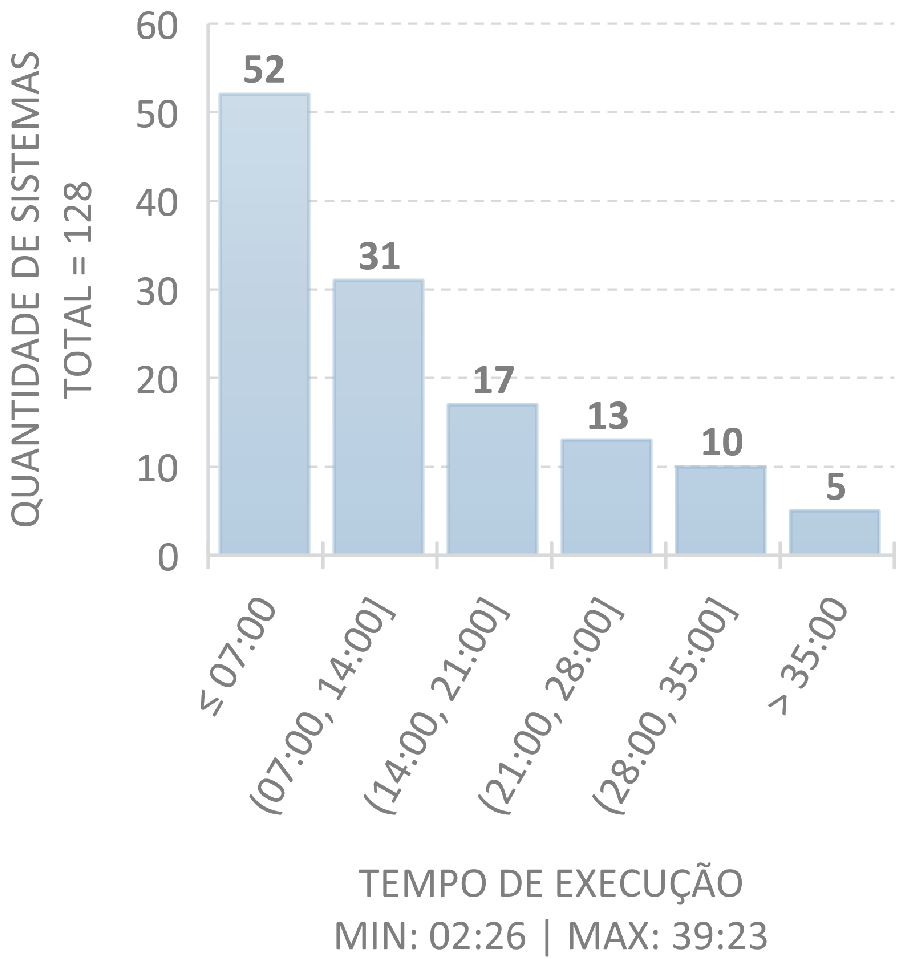
\includegraphics[width=\textwidth]{results-jmodel-timepermodel-36-stamatakis}
		\fonte{Elaborado pelo autor.}
	\end{minipage}
	\hfill
	\begin{minipage}{.52\textwidth}
		\caption{Histograma da frequência dos tempos de execução para cada um dos sistemas de substituição avaliados durante a execução do arquivo 07-primate-mtDNA no cenário $C_{j2}$.}
		\label{fig:results-jmodel-timepermodel-02-primate}
		\vspace{1ex}
		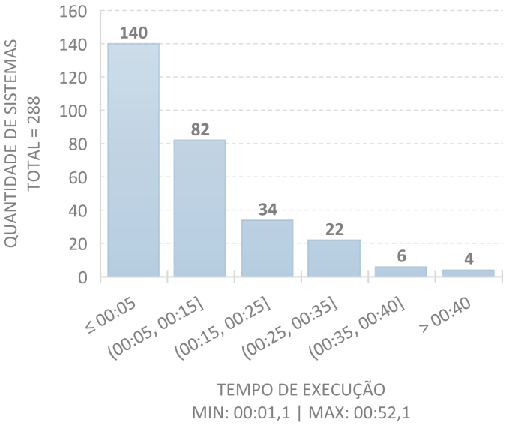
\includegraphics[width=\textwidth]{results-jmodel-timepermodel-02-primate}
		\fonte{Elaborado pelo autor.}
	\end{minipage}
\end{figure}
}



Os resultados gerais das execuções por arquivo--cenário, conforme a \autoref{tab:results-jmodel-avgs}, são apresentados de maneira visual em gráficos na \autoref{fig:results-jmodel-avgs} que adota como referência a métrica da Mediana para estipular os valores retratados.
%
Devido à amplitude dos tempos de execução a figura foi dividida em dois eixos verticais, com o eixo da direita reservado para arquivos que exigem um tempo maior de processamento, como é o caso de 12-stamatakis-59.
%
Através da representação gráfica fica evidente como o jModelTest se beneficia do aumento na quantidade de CPUs disponíveis, uma vez que este sua execução é totalmente CPU--\textit{bound}.
%
Também é possível perceber a expressiva diferença nos tempos de execução do arquivo 12-stamatakis-59 em relação ao demais onde sua execução costuma ser responsável por, em média, 63\% do tempo total de execução de cada cenário.
%
Outro destaque é o primeiro grupo de arquivos, composto por 01-aP6, 02-rodents, 03-example e 04-18S\_insects2, que contabilizam tempos de execução extremamente curtos mesmo em cenários com relativa escassez de recursos como $C_{j2}$, $C_{j4}$ e $C_{j8}$, contabilizando, somados, apenas 1\% do tempo total de execução de cada cenário.


Através da análise dos tempos de processamento por sistema de substituição molecular testado pelo jModelTest é possível verificar o caráter destas execuções em termos da sua amplitude de duração.
%
Os histogramas apresentados nas Figuras \ref{fig:results-jmodel-timepermodel-36-stamatakis} e \ref{fig:results-jmodel-timepermodel-02-primate} apresentam a frequência com que os sistemas avaliados se enquadram em um determinado intervalo de tempo de execução.
%
É possível determinar pela análise das figuras que a maior parte dos sistemas avaliados se concentra na ponta mais baixa das durações, contudo há também uma característica de cauda longa que contempla execuções que levam mais de 4x o tempo de execução da maioria.



Os resultados obtidos na coleta de execuções do jModelTest comprovam a adequação da escolha da aplicação para uso no modelo \textsf{He}--lastic, conforme definido na \autoref{sec:modelo-selecao} e explorado em detalhes na \autoref{sec:modelo-decisoes}.
%
A ampla variação no tempo de execução conforme o arquivo é uma característica relevante para o usuário do jModelTest uma vez que ele não sabe (a não ser por experiência empírica) o tempo de execução e/ou os recursos necessários para que o cálculo de adequação que está prestes a realizar.
%
Este problema torna-se ainda mais relevante em casos onde o usuário pretende executar o jModelTest em arquivos maiores, como 12-stamatakis-59, pois, uma vez que não há indicação de tempo estimado ou complexidade, não é possível saber a quantidade de recursos necessária ou adequada para requisitar em uma determinada execução supondo um ambiente de \textit{cluster} ou \textit{grid} computacional.
%
A execução local de arquivos maiores, embora sem dúvida possível, exige uma significativa dose de paciência do usuário em função dos elevados tempos de execução em computadores pessoais (que atualmente costumam ter entre 4 e 8 \textit{cores} de processamento) e até mesmo servidores de menor porte.



Ademais, o emprego da estratégia de \textit{Clustering Search}, ativada por padrão no jModelTest, faz com que a execução dos cálculos de adequação de sistemas de substituição molecular deixe de compartilhar as características de computação embaraçosamente paralela para ficar mais parecido com uma computação baseada em paralelismo do tipo BSP, conforme abordado na \autoref{fundamentacao-computacao-distribuida}.
%
Esta mudança de carácter de paralelismo torna o jModelTest ainda mais sensível ao maior esforço computacional exigido por sistemas de substituição mais complexos assim como possíveis \textit{outliers} e execuções atrasadas que acabam por determinar o tempo máximo de execução independente da média ou dos demais sistemas avaliados.
%
Embora não seja objetivo do modelo \textsf{He}--lastic atenuar ou tratar esta característica, a adoção de elasticidade pode resultar em um significativo benefício no que diz respeito ao custo financeiro uma vez que recursos ociosos serão descartados enquanto aguardam o término da computação dos sistemas de substituição mais complexos.
%
Além disso a associatividade de custos que emerge da elasticidade permite empregar um número maior de recursos durante momentos de pico enquanto mantém um custo similar ao modelo de alocação fixa por meio do descarte de recursos ociosos.


\begin{equation}
\Delta{recursos} = \dfrac{Recursos(C_{x-1})}{Recursos(C_{x})}
\end{equation}
\begin{equation}\label{eq:results-jmodel-eficiencia}
Perda = 
\left(
	\dfrac
		{Tempo(C_{x})}
		{Tempo(C_{x-1}) \times \Delta{recursos}}
\right)-1
\end{equation}


O impacto da estratégia de \textit{Clustering Search} também pode ser verificado através da análise de eficiência do jModelTest.
%
Para determinar esta métrica foram tomadas as médias dos tempos de execução por cenário e arquivo, conforme consta na \autoref{tab:results-jmodel-avgs}, e realizada a comparação entre cada cenário e o seguinte calculando-se a razão entre a diferença de tempos de execução e de recursos.
%
Desta forma é possível obter um índice normalizado, descrito na \autoref{eq:results-jmodel-eficiencia}, que expressa a perda, ou ganho, de desempenho conforme varia a quantidade de recursos disponível em cada cenário de execução.
%
Desta forma, uma execução que levava uma hora pra executar com duas unidades de recursos teria 0\% de perdas caso levasse a metade do tempo para executar com o dobro de unidades de recursos, no caso meia hora e quatro unidades.



Através da aplicação desta formula torna-se possível visualizar na \autoref{fig:results-jmodel-eficiencia} o comportamento do jModelTest em relação à sua eficiência conforme varia o uso de recursos indicando, de certa forma, seu comportamento de escalabilidade.
%
Na figura mencionada as cores determinam os cenários e a variação na quantidade de recursos e cada ponto representa um arquivo do \textit{dataset} apontando as perdas observadas pelos tempos médios de execução.
%
Como não foram observados ganhos de eficiência a figura apresenta apenas as perdas conforme variam os recursos disponíveis para cada arquivo e, destacados através dos losangos, as médias gerais para cada cenário.



\begin{figure}[bt]
	\centering%
	\begin{minipage}{\defaultFigureWidth\textwidth}
		\caption{Perda de eficiência observada durante as execuções do jModelTest através das médias dos tempos de execução por arquivo (pontos) e transição de cenários (cores) com a média geral em destaque.}
		\label{fig:results-jmodel-eficiencia}
		\vspace{1ex}
		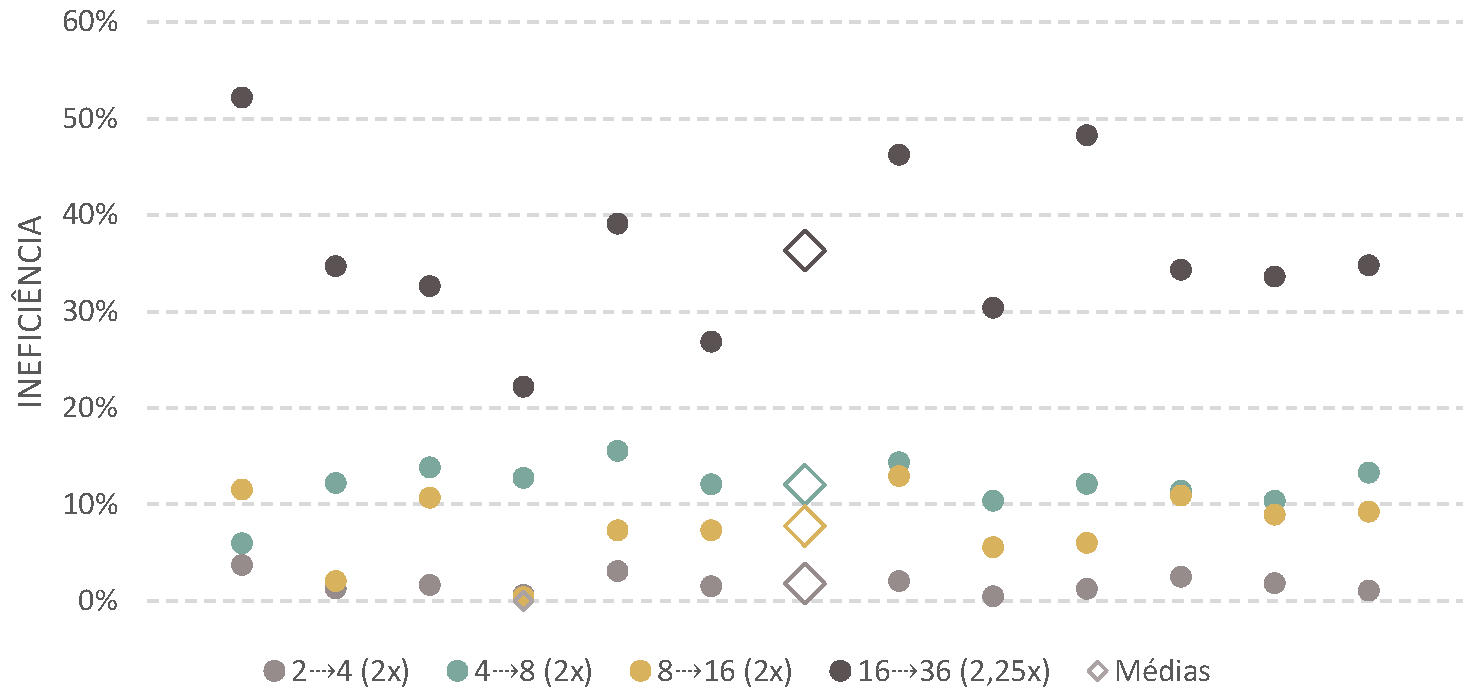
\includegraphics[width=\textwidth]{results-jmodel-eficiencia}
		\fonte{Elaborado pelo autor.}
	\end{minipage}
\end{figure}



Desta forma é possível visualizar um expressivo aumento na ineficiência na transição entre os cenários $C_{j16}$ para $C_{j36}$, reportando uma perda de, em média, 36\% apesar do aumento de 2,25x na quantidade de recursos disponíveis.
%
Enquanto isso são observadas perdas entre 12\% e 8\% para as transições entre os cenários $C_{j4}$ para $C_{j8}$ e $C_{j8}$ para $C_{j16}$ respectivamente.
%
Por fim, a transição do cenário $C_{j2}$ para $C_{j4}$ apresenta menor perda média com apenas 2\% embora a média geral dentre todos os arquivos do \textit{dataset} e cenários de teste figure em 14\% ineficiência.
%
Estes resultados corroboram com observações quanto a utilização de recursos realizadas durante o acompanhamento da execução dos cenários, onde foi possível visualizar longos períodos de recursos ociosos, neste caso \textit{cores} de processamento, conforme a execução se aproxima do final de um dos seis estágios da execução por \textit{Clustering Search} (vide \autoref{tab:modelo-elasticidade-jmodelsteps}).



Embora não seja parte dos cenários propostos na Metodologia de Avaliação, foi realizada uma única execução em uma VM dotada de 72 vCPUs para confirmar a tendência de aumento no desperdício conforme aumentam os recursos disponíveis.
%
Neste teste foi observada uma perda média, ou seja, ao longo de todos os arquivos do \textit{dataset}, de 79\% (ou 64\% excluindo o arquivo 01-aP6), um aumento expressivo frente à ineficiência de 36\% observada na transição dos cenários $C_{j16}$ para $C_{j36}$.
%
A análise de ambas as pontas do espectro no que diz respeito ao tempo de execução fornecem \textit{insights} valiosos sobre a utilização de recursos onde o arquivo 01-aP6, o menor do \textit{dataset} apresentou uma regressão, contabilizando perdas de 235\%, negando qualquer benefício do aumento de recursos uma vez que seu tempo de execução já era bastante reduzido.
%
Na ponta oposta, o arquivo 12-stamatakis-59 apresentou uma ineficiência de 43\%, contrabalanceando a maior disponibilidade de recursos com os longos períodos de ociosidade em função do processamento em fases.
%
Contudo há de se advertir que estes dados podem não refletir fielmente a realidade (principalmente nos arquivos menores) visto que o cenário foi executado apenas uma vez e desta forma servem apenas como indicativo de tendência, sem prover a confiança estatística necessária para tirar conclusões.



\begin{figure}[btp]
	\centering%
	\begin{minipage}{\textwidth}
		\caption{Utilização média de CPU ao longo de uma execução contemplando todos os arquivos do \textit{dataset} de testes em uma VM com 8 \textit{cores} de processamento equivalente ao cenário $C_{j8}$ (Duração total: 6 horas, 28 minutos).}
		\label{fig:results-jmodel-eficiencia-8}
		\vspace{1ex}
		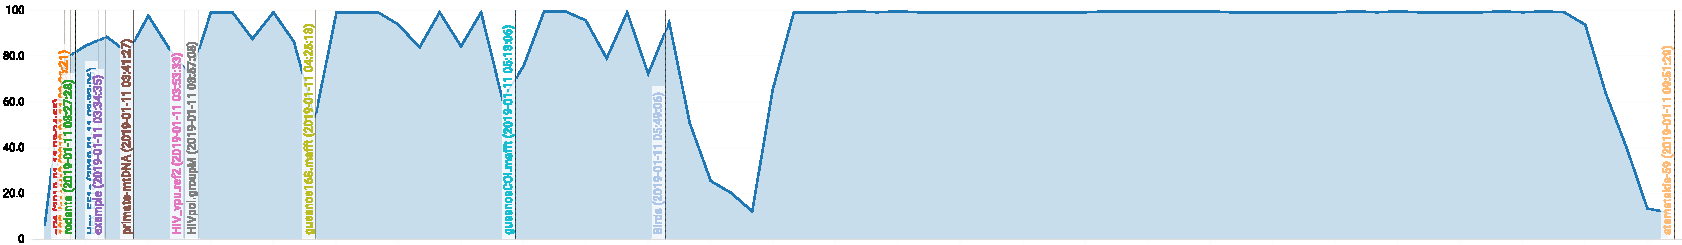
\includegraphics[width=\textwidth]{results-jmodel-eficiencia-8}
		\fonte{Capturado pelo autor a partir do serviço CloudWatch do provedor AWS.}
	\end{minipage}
	\begin{minipage}{\textwidth}
		\caption{Utilização média de CPU ao longo de execução contemplando todos os arquivos do \textit{dataset} de testes em uma VM com 16 \textit{cores} de processamento equivalente ao cenário $C_{j16}$ (Duração total: 3 horas, 44 minutos).}
		\label{fig:results-jmodel-eficiencia-16}
		\vspace{1ex}
		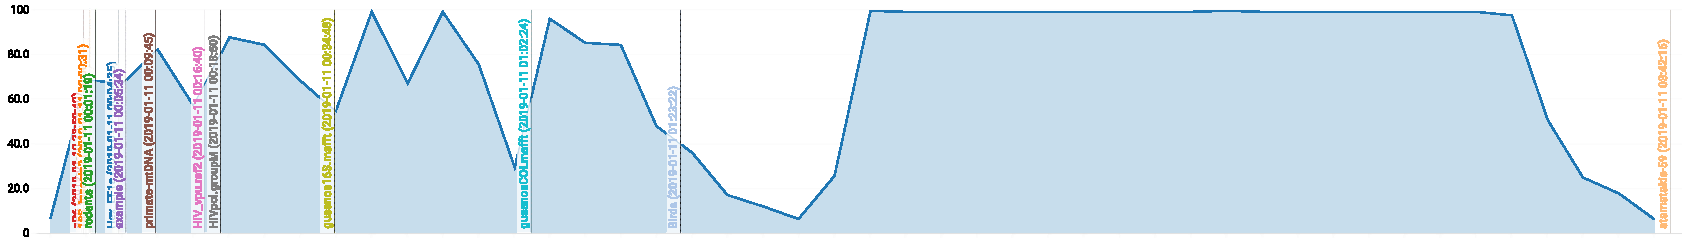
\includegraphics[width=\textwidth]{results-jmodel-eficiencia-16}
		\fonte{Capturado pelo autor a partir do serviço CloudWatch do provedor AWS.}
	\end{minipage}
	\begin{minipage}{\textwidth}
		\caption{Utilização média de CPU ao longo de uma execução contemplando todos os arquivos do \textit{dataset} de testes em uma VM com 36 \textit{cores} de processamento equivalente ao cenário $C_{j36}$ (Duração total: 2 horas, 17 minutos).}
		\label{fig:results-jmodel-eficiencia-36}
		\vspace{1ex}
		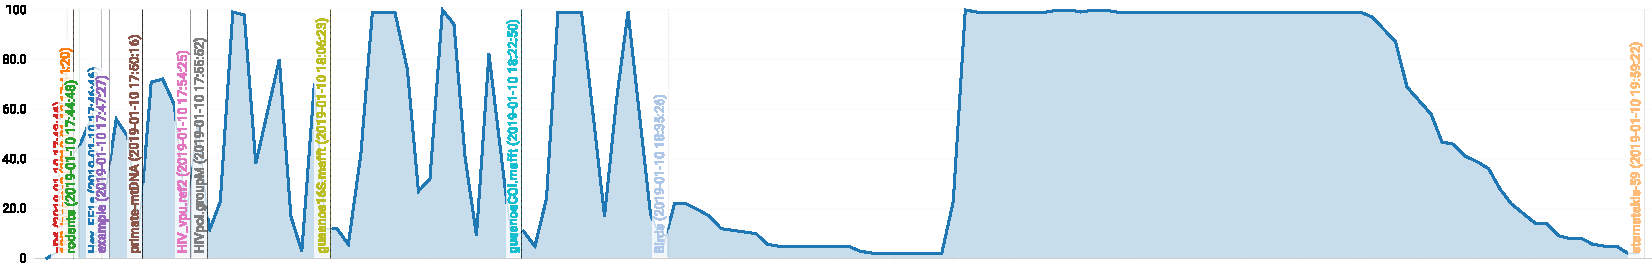
\includegraphics[width=\textwidth]{results-jmodel-eficiencia-36}
		\fonte{Capturado pelo autor a partir do serviço CloudWatch do provedor AWS.}
	\end{minipage}
	\begin{minipage}{\textwidth}
		\caption{Detalhe da \autoref{fig:results-jmodel-eficiencia-36} excluindo a execução do arquivo 12-stamatakis-59.}
		\label{fig:results-jmodel-eficiencia-36-ex12}
		\vspace{1ex}
		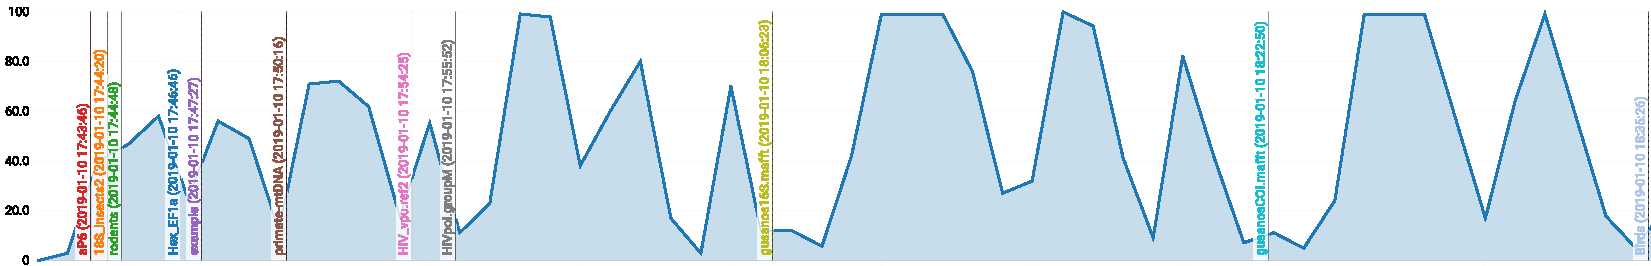
\includegraphics[width=\textwidth]{results-jmodel-eficiencia-36-ex12}
		\fonte{Capturado pelo autor a partir do serviço CloudWatch do provedor AWS.}
	\end{minipage}
	\begin{minipage}{\textwidth}
		\caption{Utilização média de CPU ao longo de uma execução contemplando os quatro maiores arquivos do \textit{dataset} de testes em uma VM com 72 \textit{cores} de processamento com o intuito de verificar o comportamento de do jModelTest  (Duração total: 1 hora, 43 minutos).}
		\label{fig:results-jmodel-eficiencia-72-maiores}
		\vspace{1ex}
		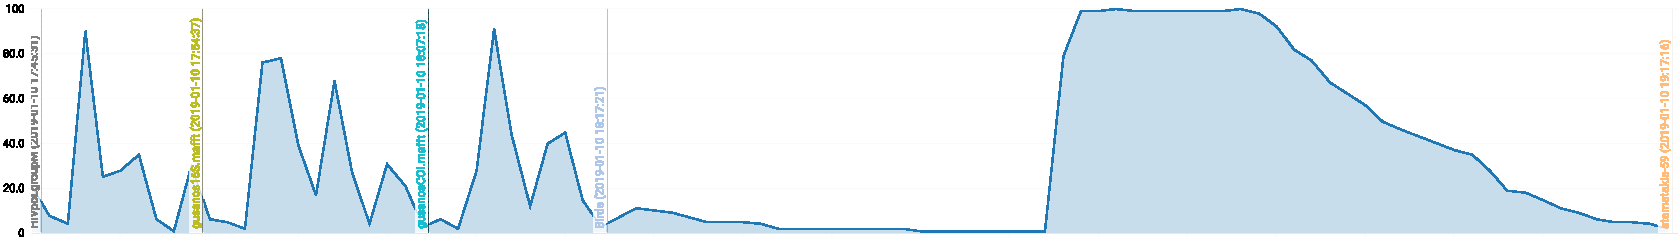
\includegraphics[width=\textwidth]{results-jmodel-eficiencia-72-maiores}
		\fonte{Capturado pelo autor a partir do serviço CloudWatch do provedor AWS.}
	\end{minipage}
\end{figure}


Para explorar os motivos das perdas de eficiência reportadas é possível recorrer às Figuras \ref{fig:results-jmodel-eficiencia-8}, \ref{fig:results-jmodel-eficiencia-16}, \ref{fig:results-jmodel-eficiencia-36} e \ref{fig:results-jmodel-eficiencia-36-ex12} que
apresentam a utilização média de CPU em períodos de um minuto conforme medida pelo provedor AWS no serviço CloudWatch enquanto ocorre uma execução completa do cenário de testes, contemplando uma única execução do jModelTest para cada arquivo do \textit{dataset}, onde 100\% equivale ao uso completo de todos os \textit{cores} disponíveis.
%
Cada linha vertical corresponde à transição entre a execução referente a um arquivo e o próximo, evidenciando o comportamento do uso de CPU durante o cálculo de adequação de sistemas de substituição molecular.
%
Na \autoref{fig:results-jmodel-eficiencia-36}, que representa uma amostra do cenário $C_{j36}$, é possível visualizar, no período que contempla os quatro últimos arquivos, por exemplo, o comportamento intermitente de uso de CPU e o desperdício de recursos em função da característica faseada do cálculo realizado através da técnica de \textit{Clustering Search}.
%
A \autoref{fig:results-jmodel-eficiencia-72-maiores} retrata uma execução em VM com 72 \textit{cores} de processamento que, embora não esteja formalmente incluída na metodologia de avaliação, suporta a intuição a respeito dos limites de escalabilidade do jModelTest haja vista sua a incapacidade de aproveitar todos os recursos disponíveis e o adiantamento da rampa descendente no uso de recursos do último arquivo, que resulta em um aumento da ociosidade. 



Os impactos da estratégia de \textit{Clustering Search} se destacam conforme aumenta a disponibilidade de recursos e principalmente no caso do último, e maior, arquivo (12-stamatakis-59) que faz uso de apenas duas fases com 8 e 120 sistemas, respectivamente, onde é possível observar um longo período de ociosidade de recursos até que todos os 8 sistemas sejam avaliados.
%
Assim que encerra o cálculo da primeira fase o programa faz uso de todos os \textit{cores} disponíveis até que se inicie, novamente, um longo período de ociosidade enquanto os últimos sistemas são processados.
%
Estes períodos de longa ociosidade são o alvo das ações de elasticidade propostas no modelo \textsf{He}--lastic por meio da camada baseada em Orquestração de Contêineres.


Através da \autoref{fig:results-jmodel-eficiencia-36-ex12}, que apresenta os mesmos dados exceto o arquivo 12-stamatakis-59, é possível observar o baixo nível de utilização média de CPU ao longo da execução do cenário apresentado.
%
O comportamento de fases, conforme detalhado na \autoref{tab:modelo-elasticidade-jmodelsteps}, torna-se ainda mais evidente assim como o desperdício observado durante a execução de arquivos menores, onde não se utiliza completamente os recursos disponíveis, o que indica uma alocação excessiva.
%
Desta forma o modelo \textsf{He}--lastic lança mão da primeira camada de elasticidade que tem como objetivo atenuar a ociosidade e consequente desperdício de recursos que ocorre ao processar arquivos menores, visando alocar apenas a quantidade necessária.





\section{Avaliação do \textsf{He}--lastic}


\begin{table}[tbp]
	\centering%
	\begin{minipage}{\textwidth}
		\caption{Quantidade de amostras coletadas na avaliação do modelo \textsf{He}--lastic para cada arquivo do \textit{dataset} conforme o cenário.}
		\label{tab:results-modelo-samples}
		\vspace{1ex}
		\footnotesize
		\begin{tabular*}{\textwidth}{@{\extracolsep{\fill}}lrrrrrrrrrrrr@{}}
			\toprule
			\multirow[b]{3}{*}{Arquivo} & \multicolumn{11}{c}{Cenário} &
			\multirow[b]{3}{*}{\rotatebox[origin=c]{\tabelaAngulo}{\begin{tabular}[c]{@{}c@{}}Total\end{tabular}}} \\ \cmidrule(lr){2-12}
			& \multicolumn{1}{c}{FaaS} & \multicolumn{3}{c}{Contêineres} & \multicolumn{7}{c}{Misto} & \multicolumn{1}{c}{} \\ 
			\cmidrule(lr){2-2}
			\cmidrule(lr){3-5}
			\cmidrule(lr){6-12}
			& $C_{f0}$ & $C_{c8}$ & $C_{c16}$ & $C_{c36}$ & $C_{m1}$ & $C_{m2}$ & $C_{m3}$ & $C_{m4}$ & $C_{m5}$ & $C_{m6}$ & $C_{m7}$ & \multicolumn{1}{c}{} \\
			\midrule
			01-aP6 & 6 & 5 & 10 & 10 & 11 & 11 & 5 & 5 & 4 & 5 & 5 & 77 \\
			02-rodents & 6 & 5 & 10 & 10 & 11 & 9 & 5 & 5 & 5 & 5 & 5 & 76 \\
			03-example & 6 & 5 & 9 & 10 & 11 & 11 & 23 & 5 & 5 & 5 & 5 & 95 \\
			04-18S\_insects2 & 6 & 5 & 5 & 5 & 11 & 11 & 5 & 5 & 5 & 5 & 5 & 68 \\
			05-HIVpol.grou[..] & 6 & 5 & 6 & 10 & 11 & 33 & 17 & 5 & 5 & 5 & 5 & 108 \\
			06-Hex\_EF1a & 6 & 5 & 5 & 9 & 11 & 32 & 5 & 5 & 5 & 5 & 5 & 93 \\
			07-primate-mtDNA & 6 & 5 & 5 & 10 & 11 & 31 & 17 & 17 & 5 & 5 & 5 & 117 \\
			08-HIV\_vpu.ref2 & 6 & 5 & 5 & 10 & 10 & 22 & 16 & 5 & 5 & 5 & 5 & 94 \\
			09-gusanos16S[..] & 5 & 5 & 5 & 10 & 11 & 13 & 11 & 5 & 5 & 11 & 5 & 86 \\
			10-Birds & 5 & 5 & 5 & 9 & 10 & 10 & 11 & 5 & 5 & 11 & 5 & 81 \\
			11-gusanosCOI[..] & 5 & 5 & 5 & 10 & 11 & 11 & 11 & 5 & 5 & 11 & 5 & 84 \\
			12-stamatakis-59 & 6 & 5 & 5 & 5 & 11 & 16 & 10 & 5 & 5 & 11 & 5 & 84 \\
			\bottomrule
			\multicolumn{1}{r}{Total} & 69 & 60 & 75 & 108 & 130 & 210 & 136 & 72 & 59 & 84 & 60 & {\scriptsize 1063} \\ 
		\end{tabular*}
		\fonte{Elaborado pelo autor.}
	\end{minipage}
\end{table}

\begin{table}[tbp]
	\centering%
	\begin{minipage}{\textwidth}
		\caption{Coeficiente de Variação (CV) na avaliação do \textsf{He}--lastic contemplando tempos de execução obtidos por arquivo e cenário de avaliação.}
		\label{tab:results-modelo-cv}
		\vspace{1ex}
		\small
		\begin{tabularx}{\textwidth}{@{\extracolsep{\fill}}lWWWWWWWWWWW@{}}
			\toprule
			\multirow[b]{3}{*}{Arquivo} & \multicolumn{11}{c}{Cenário} \\ \cmidrule(l){2-12} 
			& \multicolumn{1}{c}{FaaS} & \multicolumn{3}{c}{Contêineres} & \multicolumn{7}{c}{Misto} \\ 
			\cmidrule(lr){2-2}
			\cmidrule(lr){3-5}
			\cmidrule(l){6-12}
			& $C_{f0}$ & $C_{c8}$ & $C_{c16}$ & $C_{c36}$ & $C_{m1}$ & $C_{m2}$ & $C_{m3}$ & $C_{m4}$ & $C_{m5}$ & $C_{m6}$ & $C_{m7}$ \\ 
			\midrule
			01-aP6 & 9\% & 22\% & 10\% & 15\% & 9\% & 6\% & 5\% & 5\% & 5\% & 0\% & 12\% \\
			02-rodents & 8\% & 3\% & 11\% & 6\% & 7\% & 11\% & 17\% & 7\% & 7\% & 8\% & 2\% \\
			03-example & 3\% & 20\% & 12\% & 15\% & 3\% & 12\% & 9\% & 8\% & 8\% & 3\% & 9\% \\
			04-18S\_insects2 & 3\% & 8\% & 9\% & 5\% & 3\% & 9\% & 10\% & 6\% & 9\% & 6\% & 9\% \\
			05-HIVpol.groupM & 4\% & 3\% & 11\% & 7\% & 5\% & 6\% & 3\% & 5\% & 6\% & 4\% & 11\% \\
			06-Hex\_EF1a & 5\% & 7\% & 10\% & 18\% & 7\% & 5\% & 6\% & 5\% & 4\% & 5\% & 4\% \\
			07-primate-mtDNA & 4\% & 5\% & 8\% & 8\% & 5\% & 5\% & 5\% & 40\% & 7\% & 9\% & 5\% \\
			08-HIV\_vpu.ref2 & 18\% & 18\% & 9\% & 8\% & 18\% & 16\% & 20\% & 11\% & 2\% & 16\% & 2\% \\
			09-gusanos16S.mafft & 0\% & 5\% & 4\% & 9\% & 7\% & 4\% & 8\% & 9\% & 6\% & 12\% & 6\% \\
			10-Birds & 0\% & 4\% & 8\% & 7\% & 18\% & 3\% & 16\% & 7\% & 6\% & 19\% & 1\% \\
			11-gusanosCOI.mafft & 0\% & 4\% & 10\% & 11\% & 1\% & 6\% & 2\% & 5\% & 7\% & 7\% & 2\% \\
			12-stamatakis-59 & 0\% & 2\% & 1\% & 5\% & 2\% & 15\% & 3\% & 7\% & 6\% & 4\% & 6\% \\ 
			\bottomrule
		\end{tabularx}
		\fonte{Elaborado pelo autor.}
	\end{minipage}
\end{table}


Os resultados do modelo \textsf{He}--lastic, coletados por meio do protótipo desenvolvido, seguem os mesmos moldes dos cenários de avaliação centrados no jModelTest.
%
Esta estratégia visa estabelecer uma comparação o mais fiel possível enquanto não deixa de endereçar as diferenças existente entre as abordagens avaliadas, principalmente no que diz respeito à camada FaaS do modelo proposto.
%
Desta forma foram avaliados, assim como na seção anterior, os cenários de testes estabelecidos na \autoref{sec:metodologia-etapasecenarios}
e apresentados na \autoref{tab:results-modelo-samples} que apresenta os resultados da coleta de dados baseada na execução do protótipo do modelo \textsf{He}--lastic, totalizando, após filtragem de anomalias (\textit{outliers}), 1063 execuções por arquivo--cenário.
%
Para obter a quantidade de chamadas à ferramenta PhyML basta multiplicar os dados da \autoref{tab:results-jmodel-samples} pela \autoref{tab:metodologia-etapas-dataset}, mais especificamente a quantidade de sistemas de substituição molecular contemplados por arquivo quando é seguida a estratégia de \textit{Clustering Search}, resultando em aproximadamente 270 mil (268.992) execuções por arquivo--sistema--cenário.


Apesar do número similar de execuções em relação às avaliações do jModelTest, nos testes do modelo proposto foi necessário reduzir a quantidade de amostras para viabilizar a execução de todos os cenários propostos.
%
Desta forma foi estabelecido que cinco seria o número mínimo desejado de amostras, menor que os onze desejados na avaliação do jModelTest, contudo ainda significativos o suficiente para fornecer uma rede de segurança estatística para que se possam tirar conclusões acerca dos resultados.
%
Os pontos de maior concentração no número de amostras coletadas indicam áreas de interesse devido ao comportamento dinâmico em duas camadas do modelo ou cenários que apresentavam alta variação nos tempos de execução e receberam maior atenção para garantir uma melhor compreensão do comportamento.


\afterpage{
	\clearpage
	\begin{landscape}
		\begin{table}[tbp]
			\centering%
			\begin{minipage}{\linewidth}
				\caption{Mediana dos tempos de execução observados no modelo \textsf{He}--lastic por arquivo e cenário de avaliação.}
				\label{tab:results-modelo-avgs}
				\vspace{0.75ex}
				\small
				\renewcommand\arraystretch{1.35}
				\begin{tabularx}{\textwidth}{@{\extracolsep{\fill}}lWWWWWWWWWWW@{}}
					\toprule
					\multirow{3}{*}{Arquivo} & \multicolumn{11}{c}{Tempo de Execução (Mediana) / Cenário} \\ \cmidrule(l){2-12} 
					& \multicolumn{1}{c}{FaaS} & \multicolumn{3}{c}{Contêineres} & \multicolumn{7}{c}{Misto} \\ 
					\cmidrule(lr){2-2}
					\cmidrule(lr){3-5}
					\cmidrule(l){6-12}
					& $C_{f0}$ & $C_{c8}$ & $C_{c16}$ & $C_{c36}$ & $C_{m1}$ & $C_{m2}$ & $C_{m3}$ & $C_{m4}$ & $C_{m5}$ & $C_{m6}$ & $C_{m7}$ \\ 
					\midrule
					01-aP6 & 0:00:09 & 0:23:14 & 0:13:46 & 0:09:48 & 0:00:09 & 0:00:11 & 0:00:12 & 0:00:09 & 0:00:09 & 0:00:11 & 0:00:12 \\
					02-rodents & 0:00:13 & 0:19:49 & 0:12:03 & 0:09:07 & 0:00:12 & 0:00:14 & 0:00:13 & 0:00:12 & 0:00:12 & 0:00:14 & 0:00:22 \\
					03-example & 0:00:27 & 0:22:42 & 0:13:04 & 0:10:04 & 0:00:24 & 0:00:24 & 0:00:27 & 0:00:21 & 0:00:24 & 0:00:27 & 0:00:45 \\
					04-18S\_insects2 & 0:00:19 & 0:20:28 & 0:11:40 & 0:09:20 & 0:00:20 & 0:00:16 & 0:00:20 & 0:00:17 & 0:00:17 & 0:00:20 & 0:00:28 \\
					05-HIVpol.groupM & 0:00:30 & 0:19:49 & 0:12:16 & 0:08:54 & 0:00:27 & 0:00:27 & 0:00:33 & 0:00:28 & 0:00:28 & 0:00:32 & 0:00:56 \\
					06-Hex\_EF1a & 0:01:00 & 0:19:59 & 0:13:07 & 0:08:32 & 0:00:58 & 0:01:00 & 0:00:57 & 0:00:56 & 0:01:01 & 0:01:02 & 0:01:41 \\
					07-primate-mtDNA & 0:01:37 & 0:22:37 & 0:13:58 & 0:10:41 & 0:01:35 & 0:01:35 & 0:01:33 & 0:04:06 & 0:01:35 & 0:01:43 & 0:02:45 \\
					08-HIV\_vpu.ref2 & 0:04:11 & 0:25:41 & 0:15:23 & 0:11:14 & 0:04:03 & 0:13:01 & 0:04:04 & 0:33:17 & 0:34:10 & 0:06:36 & 0:36:58 \\
					09-gusanos16S.mafft & --- & 0:33:44 & 0:18:57 & 0:13:04 & 0:45:18 & 0:34:59 & 0:36:11 & 0:31:10 & 0:33:45 & 0:39:14 & 0:39:43 \\
					10-Birds & --- & 0:21:52 & 0:13:04 & 0:09:08 & 0:15:09 & 0:15:13 & 0:15:24 & 0:24:16 & 0:24:06 & 0:16:46 & 0:27:33 \\
					11-gusanosCOI.mafft & --- & 0:52:04 & 0:30:46 & 0:19:01 & 1:20:06 & 0:55:15 & 0:58:15 & 0:42:48 & 0:48:09 & 0:58:09 & 0:57:34 \\
					12-stamatakis-59 & --- & 3:25:39 & 1:54:33 & 1:06:10 & 3:38:43 & 1:39:45 & 2:13:11 & 1:14:59 & 1:17:30 & 1:21:56 & 1:17:19 \\ 
					\bottomrule
				\end{tabularx}
				\fonte{Elaborado pelo autor.}
			\end{minipage}
		\end{table}
	\end{landscape}
}



No que diz respeito ao Coeficiente de Variação pode-se perceber através dos dados da \autoref{tab:results-modelo-cv} que houve um evidente aumento.
%
Esta mudança no comportamento da métrica CV pode ser explicada pela redução na quantidade de execuções, cujos objetivos caíram de 11 para 5 em função do aumento na variedade de cenários avaliados.
%
Além disso é possível perceber que algumas combinações geram resultados atípicos como as tuplas [07-primate-mtDNA, $C_{m4}$], [01-aP6, $C_{c8}$], [03-example, $C_{c8}$], [08-HIV\_vpu.ref2, $C_{m3}$], com CVs de 40\%, 22\%, 20\% e 20\%.
%
A respeito da combinação 07-primate-mtDNA--$C_{m4}$, com 40\% de CV a explicação se dá pela agressiva redução no tempo limite de execução (\textit{timeout}) para a camada FaaS, que passou de 60s na maioria dos cenários para apenas 15s.
%
Esta ampla variação pode se originar em função de uma aproximação do tempo limite de execução com o tempo médio de execução de cada teste de adequação de sistemas de substituição molecular gerando \textit{retries} que, devido a existência de uma camada de \textit{caching} de recursos presente no FaaS, permite que as execuções subsequentes sejam mais rápidas.
%
Outra possibilidade é a pura variação nos patamares de performance entregue pela camada FaaS que, embora seja a mais confiável dentre os grandes provedores de computação em nuvem \cite{Wang2018}, ainda demonstra ampla variação nos recursos subjacentes como demonstrou a \autoref{tab:metodologia-infra-lambdacpus}.



Contudo, assim cono nas execuções do jModelTest é possível afirmar que as estatísticas mostram uma distribuição concentrada nos pontos centrais como média e mediana.
%
A métrica de Variância, nas execuções do modelo \textsf{He}--lastic também permaneceu zerada para a maior parte das 132 combinações cenário--arquivo, apenas apresentando valores de: dez segundos para a combinação 12-stamatakis-59 cenário $C_{m2}$, dois segundos para a combinação 01-aP6 cenário $C_{c8}$ e apenas um segundo para outras 6 combinações, totalizando somente 6\% de ocorrências maiores que zero.
%
A ampla variância do arquivo 12-stamatakis-59 no cenário $C_{m2}$ pode ser explicada por sua execução acontecer sempre apenas na camada de Orquestração de Contêineres, devido à incapacidade da camada FaaS de absorver as requisições por falta de potência e tempo hábil de processamento.
%
Desta forma existe uma injeção de ruído no tempo de execução oriunda das ações de elasticidade do Orquestrador de Contêineres ao adicionar e remover recursos que é potencializada com a variação adicional decorrente da aplicação da política de \textit{retry} por \textit{backoff} exponencial imposta pelo provedor AWS, e descrita em detalhes na \autoref{sec:metodologia-prototipo-dificuldades}. 


Uma análise da \autoref{tab:results-modelo-avgs} permite identificar três comportamentos distintos que se manifestam através das medianas do tempo total de execução de cada cenário.
%
Ao visualizar na \autoref{fig:results-modelo-caracteristicas} os dados de registros de execução, normalizados através do cálculo do percentual do tempo máximo de execução e ordenados pelo seu valor numérico é possível perceber três grupos de comportamentos bem definidos e distintos entre si.
%
Entretanto, o surgimento de três \textquoteleft famílias\textquoteright de comportamento não surpreende uma vez que este é o mesmo resultado que emerge da combinação entre as camadas de elasticidade e, por consequência, os cenários de avaliação, comprovando, também, a relevância da estratégia de duas camadas de elasticidade adotada pelo modelo \textsf{He}--lastic, uma vez que as características da interação entre as duas camadas dá origem a um comportamento que é visivelmente diferente daquele demonstrado pelas demais camadas de elasticidade quando funcionando de maneira isolada.


\begin{figure}[bt]
	\centering%
	\begin{minipage}{\defaultFigureWidth\textwidth}
		\caption{Gráfico de evolução do tempo de execução observado a cada arquivo e cenário quando expressados e ordenados em termos do percentual do tempo máximo de execução.}
		\label{fig:results-modelo-caracteristicas}
		\vspace{1ex}
		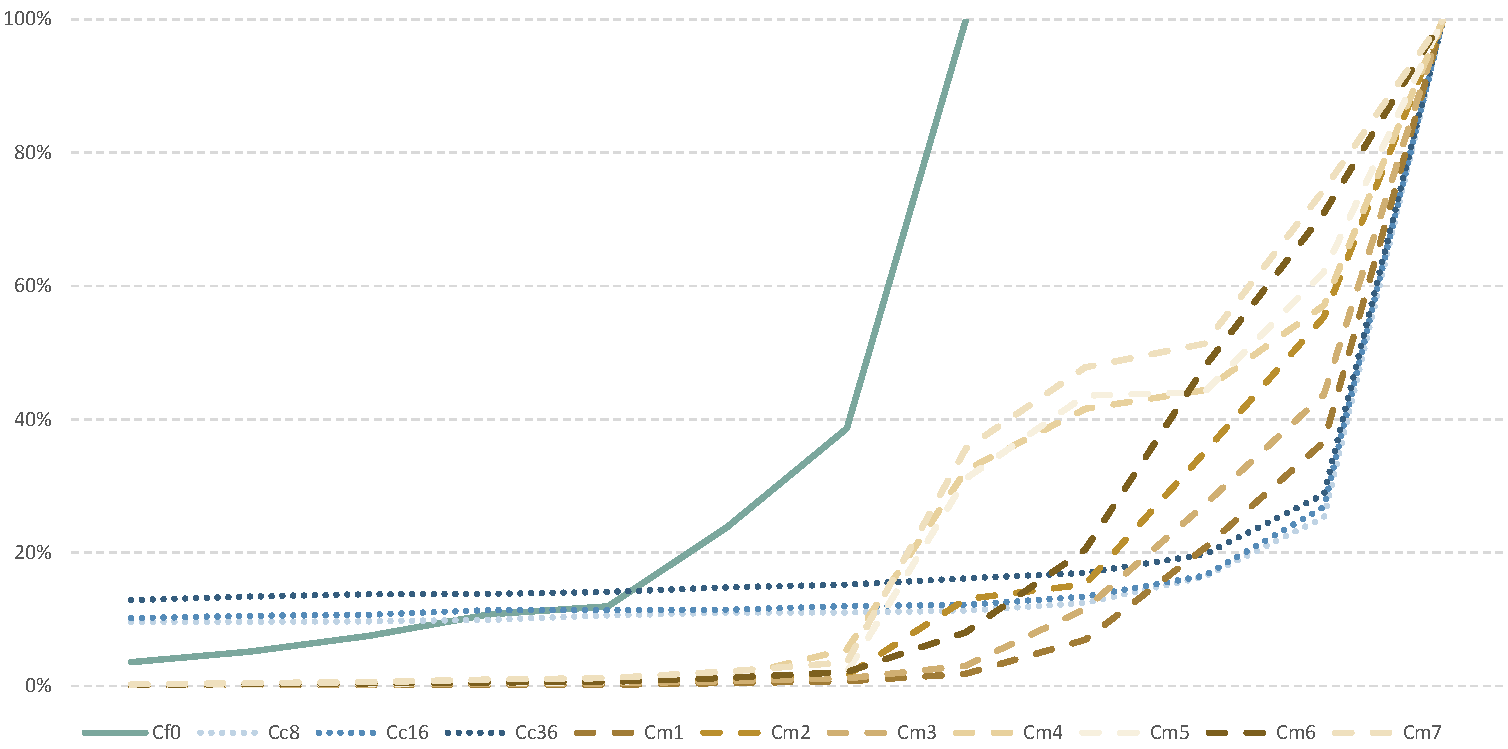
\includegraphics[width=\textwidth]{results-modelo-caracteristicas}
		\fonte{Elaborado pelo autor.}
	\end{minipage}
\end{figure}



Representado pela linha verde contínua, o cenário apenas FaaS ($C_{f0}$) se destaca dos demais ao atingir a marca de 100\% antes dos restantes, um comportamento que se origina da incapacidade de concluir o processamento de todos os arquivos do \textit{dataset} devido às restrições impostas pelo modelo FaaS no que diz respeito ao uso de recursos e tempo de execução.
%
As linhas azuis pontilhadas representam o grupo baseado na Orquestração de Contêineres, contemplando os cenários {$C_{c8}$, $C_{c16}$ e $C_{c36}$}, onde é possível observar que as primeiras execuções, apesar de compartilhar a progressividade característica dos arquivos contemplados no \textit{dataset}, partem de um patamar mais elevado do que às demais.
%
Embora os patamares iniciais entre os grupos somente FaaS e somente Contêineres não pareçam tão distantes, uma análise dos dados absolutos via \autoref{tab:results-modelo-avgs} revela que há, de fato, uma larga distância entre eles, sendo o fenômeno observado no gráfico um resultado da relativização em termos do percentual do tempo total de execução.
%
Para compreender melhor as origens dos três comportamentos distintos, uma análise detalhada é apresentada a seguir.

%\begin{verbatim}
%cenário new
%amostras
%std-dev
%durations
%\end{verbatim}






\subsection{Cenário Somente FaaS}
\label{sec:resultados-modelo-faas}



O paradigma Function as a Service / Serverless permite a simplificação do ambiente das configurações, promete amplo paralelismo e fornece faturamento contabilizado em unidades de 100ms, o que garantiu grande popularidade e adoção no meio comercial.
%
Em contrapartida, nos ambientes acadêmicos ainda são encontradas poucas referências e análises a respeito do assunto, comprovando a necessidade de estudo e melhor caracterização deste modelo computacional.
%
Desta forma o cenário Somente FaaS ($C_{f0}$) foi incluído no conjunto de cenários da metodologia de avaliação com o intuito de viabilizar um melhor conhecimento a respeito e verificar os níveis de impacto que podem ser causados pela escolha de FaaS.



A execução do cenário $C_{f0}$ teve configurados os seguintes parâmetros: Potência/Memória e Tempo Limite com os valores de 1536 e 60, respectivamente.
%
A escolha dos parâmetros não é por acaso haja vista que é ele que determina o limite superior aos parâmetros das execuções dos cenários Mistos, uma decisão que tem por objetivo permitir uma comparação justa entre os cenários e facilitar a identificação de \textit{overhead} ou interferências do modelo proposto.



Um dos pontos mais convincentes sobre a adoção de FaaS está na sua capacidade de responder rapidamente à mudanças na carga de trabalho através do lançamento de novas unidades de execução.
%
Determinar o número de processadores, processos ou contêineres envolvidos na execução é, sem dúvida, um fator relevante para este e outros trabalhos.
%
Através da extração de \textit{logs} do serviço CloudWatch do provedor de computação em nuvem escolhido é possível capturar o identificador da unidade de execução, geralmente chamado de contêiner ou instância, embora ambos os termos já representem outros conceitos.
%
De posse destes identificadores torna-se possível contabilizar as unidades de execução e verificar questões como reuso e grau de paralelismo na execução dos cenários de avaliação.
%
A fim de reduzir possíveis equívocos foi adotado o nome de Processos, que representam, portanto, a quantidade de unidades distintas de execução alocadas pelo provedor para servir requisições.



A \autoref{tab:results-modelo-faas-computacao} apresenta, sumarizados através das médias, os resultados encontrados para este cenário assim como uma comparação com o cenário de recursos fixos baseado no jModelTest.
%
A comparação da razão entre os tempos de execução e os tempos médios observados pelos cenários $C_{j2}$ e $C_{j36}$ contempla os dois extremos do espectro que avaliou a execução do jModelTest na \autoref{sec:resultados-jmodel} e permite detectar o impacto de performance ocasionado pelo uso da tecnologia FaaS.
%
São detectados, nesta análise, três casos onde o \textit{overhead} da tecnologia FaaS causou um atraso ou impactou a performance da execução sendo, nomeadamente: 
\begin{inparaenum}[\itshape a\upshape)] 
	\item 01-aP6;
	\item 03-example; e
	\item 08-HIV\_vpu.ref2.
\end{inparaenum}


\begin{table}[tb]
	\centering%
	\begin{minipage}{\textwidth}
		\caption{Processos e Tempo de Execução médios do cenário somente FaaS ($C_{f0}$) do modelo \textsf{He}--lastic.}
		\label{tab:results-modelo-faas-computacao}
		\vspace{1ex}
		%\small
		\begin{tabularx}{\textwidth}{@{\extracolsep{\fill}}lrrrrrr@{}}
			\toprule
			&  &  &  & \multicolumn{3}{c}{Percentual Sobre} \\ \cmidrule(l){5-7} 
			& Processos & CPU--time & Execução & CPU--time & $C_{j2}$ & $C_{j36}$ \\ \midrule
			01-aP6 & 63 & 0:01:31 & 0:00:09 & 10\% & 23\% & 223\% \\
			02-rodents & 114 & 0:04:34 & 0:00:13 & 5\% & 7\% & 75\% \\
			03-example & 118 & 0:06:51 & 0:00:27 & 6\% & 9\% & 100\% \\
			04-18S\_insects2 & 117 & 0:06:21 & 0:00:19 & 5\% & 6\% & 83\% \\
			05-HIVpol.groupM & 120 & 0:11:56 & 0:00:30 & 4\% & 4\% & 42\% \\
			06-Hex\_EF1a & 120 & 0:22:34 & 0:00:59 & 4\% & 5\% & 57\% \\
			07-primate-mtDNA & 120 & 0:34:26 & 0:01:37 & 5\% & 7\% & 62\% \\
			08-HIV\_vpu.ref2 & 122 & 1:42:02 & 0:04:41 & 5\% & 10\% & 121\% \\
			\bottomrule
			\multicolumn{1}{r}{Média Geral} & 112 & --- & --- & 5\% & 8\% & 84\% \\ 
		\end{tabularx}
		%\tabelafootnote{{*}~Valores obtidos através da média das execuções.}
		\fonte{Elaborado pelo autor.}
	\end{minipage}
\end{table}


No que diz respeito ao arquivo 01-aP6, embora o valor percentual de 223\% possa assustar, esta variação se deve ao pequeno valor absoluto, menor que dez segundos e, portanto, muito sensível à variações, mesmo que não sejam significativas para o usuário, como é o caso aqui.
%
Já no caso do arquivo 03-example as médias dos tempos de execução via FaaS foram praticamente iguais aos do cenário $C_{j36}$, com durações de 27 e 26 segundos, respectivamente, um resultado que pode ser considerado ainda satisfatório considerando-se o alto nível de paralelismo obtido através dos quase 120 processos mais de 3 vezes o observado no cenário $C_{j36}$, que estava limitado a 36 \textit{cores}.
%
O arquivo 08-HIV\_vpu.ref2 apresenta uma situação interessante que se manifesta no impacto de aproximadamente 20\% na performance quando comparada ao cenário $C_{j36}$ e que pode ser explicado pela ocorrência de \textit{retries}, detectável através do número maior de processos paralelos (122) do que o paralelismo máximo (120) dos estágios de processamento do jModelTest, como detalhado na \autoref{tab:modelo-elasticidade-jmodelsteps}.




A existência de \textit{retries} durante o processamento indica a proximidade com os limites estabelecidos para a camada FaaS no cenário $C_{f0}$, onde os recursos alocados não são mais suficientes para dar conta do processamento solicitado.
%
Contudo, mesmo se aproximando do ponto de saturação e excedendo o tempo limite em alguns processos, é interessante notar que o arquivo ainda é processado integralmente, o que parece contra intuitivo uma vez que não houve alteração nos parâmetros estabelecidos para o cenário.
%
Este fenômeno pode ser explicado por duas características que trabalham juntas e influenciam o tempo de execução de cada processo paralelo, sendo a primeira delas as pequenas variações de performance que ocorrem em função da virtualização e de fatores fora do controle da função FaaS como \textit{scheduler} de sistema operacional e contenção de leitura e escrita.
%
A segunda característica é a existência de um \textit{cache} na camada FaaS que evita a necessidade de obter um novo ambiente de execução e até mesmo os arquivos de entrada que também ficam em \textit{cache} em área temporária de armazenamento, o que acelera de maneira significativa uma reexecução ao remover a necessidade de buscar recursos remotos.



Ainda assim, no resultado geral obtido, é possível dizer que o cenário com apenas FaaS obteve tempos de execução em linha com as execuções do jModelTest com 36 \textit{cores} do cenário $C_{j36}$, alcançando uma duração de 84\%, na média entre os arquivos que ele foi capaz de processar integralmente.
%
Quando comparado com o cenário de apenas dois \textit{cores}, $C_{j2}$ a execução via FaaS levou, em média, somente 8\% do tempo total observado, uma significativa melhoria obtida através do alto grau de paralelismo possibilitado pelo uso da camada FaaS.
%
A respeito do paralelismo é possível observar que se manteve muito próximo do limite de 120 estabelecido pela execução em fases do jModelTest, com a média geral em 112 processos paralelos em execução, confirmando a capacidade da camada FaaS de obter rapidamente o alto nível de paralelismo prometido, onde impressiona o resultado do arquivo 02-rodents onde foram observados 114 processos paralelos em apenas 13 segundos de execução total.



No que tange ao tempo de execução em relação ao tempo total de processamento utilizado, chamado na \autoref{tab:results-modelo-faas-computacao} de CPU--time, é possível perceber que este se mantém estável em torno de 5\% no geral, com a notável exceção sendo o arquivo 01-aP6 que reporta um tempo de execução de 10\% do tempo total de processamento.
%
A relativa estabilidade deste indicador pode ser explicada devido a natureza do processamento realizado pelo jModelTest e pelo protótipo do modelo \textsf{He}--lastic, onde cada processo paralelo é responsável por executar o cálculo de \textit{best--fit} de sistemas de substituição molecular.
%
Neste caso, os sistemas executados são sempre os mesmos e a variação se dá através do arquivo de múltiplos alinhamentos de sequências, conforme definidos na \autoref{sec:metodologia-etapasecenarios}, de forma que o sistema com maior tempo de duração do cálculo acaba se tornando balizador do tempo de execução, uma vez que todas as durações são proporcionais ao arquivo fornecido como parâmetro de entrada.



Por fim é importante notar que a grande vantagem da execução via FaaS, e do modelo \textsf{He}--lastic, está na sua capacidade de cobrar apenas pelo tempo efetivo de execução, sendo este o grande fator de diferenciação quando comparado com os cenários de base do jModelTest, que se apoiam na existência de servidores, \textit{grids} ou \textit{clusters} computacionais sempre disponíveis.
%
A comparação dos tempos de execução indica que, embora exista um \textit{overhead} oriundo da adoção do FaaS, uma vez que seu tempo de execução empregando mais de cem processos foi praticamente o mesmo do que o jModelTest com apenas 36 \textit{cores}, este \textit{overhead} não é significativo o suficiente para justificar o abandono do FaaS como alternativa viável.
%
Soma-se a isto o fato observado na \autoref{sec:resultados-jmodel} de que o jModelTest tende a perder eficiência conforme aumentam os recursos disponíveis, 
causando retornos decrescentes no investimento em hardware.
%
Contudo é evidente, também, que a computação via FaaS tem suas falhas, manifestando-se claramente na incapacidade de processar os arquivos maiores do \textit{dataset} em função dos limites de potência e tempo de execução.
%
Ademais, ainda que estes limites fossem flexibilizados, eventualmente o custo monetário, conforme visto na \autoref{sec:modelo-custben}, tornaria sua utilização proibitiva, uma vez que o objetivo dos provedores de computação em nuvem com este tipo de serviço é incentivar a rotatividade através de curtas execuções, o que inviabiliza sua adoção como plataforma de computação de propósito geral.








\subsection{Cenário Somente Orquestrador de Contêineres}


Ao contrário do FaaS, a elasticidade por regra--condição--ação, utilizada pelo Orquestrador de Contêineres já encontra-se estabelecida tanto no meio comercial quanto acadêmico, sendo um dos pilares da computação em nuvem.
%
As avaliações realizadas nos cenários compostos somente por Orquestração de Contêineres buscaram verificar o comportamento dinâmico da elasticidade e o seu impacto de performance frente a execuções do jModelTest em um ambiente não distribuído com paralelismo obtido por meio de \textit{threads}.
%
Através desta metodologia é possível observar o impacto na performance e consequente \textit{overhead} computacional pelo emprego da elasticidade frente a um cenário ótimo do jModelTest, uma vez que a execução por \textit{threads} causa o menor impacto quando comparada com a computação distribuída por MPI, por exemplo.


O uso do serviço Batch, do provedor AWS, como gestor de elasticidade embora não permita a explícita configuração dos \textit{thresholds} mínimos e máximos comumente adotados para controle da elasticidade, faz uso destas configurações internamente, juntamente com informações a respeito do nível de ocupação da fila de trabalhos aguardando processamento.
%
Esta estratégia, embora não seja estritamente igual a elasticidade como geralmente definida na literatura, representa uma arquitetura comum à diversos projetos que fazem uso da elasticidade para compor \textit{pipelines} de processamento distribuído e desacoplados, utilizando filas de mensagens em conjunto com ações de elasticidade.
%
Sendo considerado, portanto, adequado para os fins deste trabalho uma vez que facilita a configuração e integração dos diferentes passos de processamento adotados pelo modelo \textsf{He}--lastic.


Ao embutir, em suas informações de contexto, dados a respeito do estado da fila de trabalhos, o serviço Batch permite, assim como o Lambda no FaaS, descartar completamente a necessidade de recursos ociosos enquanto aguarda novas requisições.
%
Esta propriedade é também utilizada pelo modelo \textsf{He}--lastic para prover uma computação ainda mais próxima do modelo pague pelo uso (\textit{pay--per--use}) objetivada pelo conceito de \textit{utility--computing}.
%
Em cenários de elasticidade, mesmo que não haja demanda sendo exercida em um determinado momento, é prática comum manter disponível pelo menos um nível mínimo de recursos computacionais para atender requisições que possam chegar, evitando o risco de rejeitar conexões e aparentar estar indisponível.
%
Embora esta não seja uma preocupação para grandes aplicações de uso contínuo, pode significar maior economia em cenários de baixa demanda ou sazonais, que contemplem longos períodos de ociosidade, por exemplo.


A fim de possibilitar uma comparação justa frente aos cenários de avaliação do jModelTest, os testes da camada de Orquestração de Contêineres do modelo \textsf{He}--lastic contemplaram três cenários variando o parâmetro de número máximo de CPUs utilizadas, uma vez que, conforme anteriormente mencionado, não há a necessidade de configurar \textit{thresholds} ao utilizar o serviço AWS Batch.
%
Desta forma foram estabelecidos os cenários $C_{c8}$, $C_{c16}$ e $C_{c36}$ com limites máximos de 8, 16 e 36 CPUs, respectivamente.
%
Estes cenários podem ser diretamente comparados com os cenários de avaliação do jModelTest $C_{j8}$, $C_{j16}$ e $C_{j36}$ para uma análise dos impactos de performance obtidos através da adoção de elasticidade e do serviço AWS Batch.


Conforme observado previamente na \autoref{fig:results-modelo-caracteristicas}, através das linhas pontilhadas de tonalidade azul, que representam os cenários com somente o Orquestrador de Contêineres, é observado um fenômeno interessante no processamento dos arquivos menores.
%
Pela análise da figura é possível visualizar uma reta quase plana que contempla os arquivos de 01-aP6 ao 10-Birds e que se mantém com um tempo de execução entre 10\% à 20\% do tempo total.
%
Este comportamento também pode ser observado pela análise da \autoref{tab:results-modelo-avgs}, que mostra em valores absolutos as medianas dos tempos de execução observados para os cenários aqui analisados, onde é possível perceber que, na média, os tempos de execução dos arquivos de 01 à 10 do cenário $C_{c8}$ giram em torno de 24 minutos, no cenário $C_{c16}$ em 14 minutos e, finalmente, no cenário $C_{c36}$ giram em torno de 10 minutos.


\begin{table}[tb]
	\centering%
	\begin{minipage}{\textwidth}
		\caption{Tempos de Execução médios dos cenários somente Orquestrador de Contêineres do modelo \textsf{He}--lastic.}
		\label{tab:results-modelo-batch-computacao}
		\vspace{1ex}
		%\small
		\begin{tabularx}{\textwidth}{@{\extracolsep{\fill}}lrrrrrr@{}}
			\toprule
			\multicolumn{1}{c}{\multirow{2}{*}{Arquivo}} &  &  &  & \multicolumn{3}{c}{Percentual Sobre} \\ \cmidrule(l){5-7} 
			\multicolumn{1}{c}{} & $C_{c8}$ & $C_{c16}$ & $C_{c36}$ & $C_{j8}$ & $C_{j16}$ & $C_{j36}$ \\ 
			\midrule
			01-aP6 & 0:27:00 & 0:13:37 & 0:10:03 & 14613\% & 13223\% & 14408\% \\
			02-rodents & 0:19:44 & 0:12:06 & 0:09:06 & 2083\% & 2503\% & 3144\% \\
			03-example & 0:25:58 & 0:13:42 & 0:10:14 & 1908\% & 1819\% & 2305\% \\
			04-18S\_insects2 & 0:21:14 & 0:12:06 & 0:09:23 & 1541\% & 1763\% & 2519\% \\
			05-HIVpol.groupM & 0:19:50 & 0:12:48 & 0:08:55 & 556\% & 669\% & 754\% \\
			06-Hex\_EF1a & 0:20:54 & 0:13:35 & 0:08:28 & 363\% & 440\% & 486\% \\
			07-primate-mtDNA & 0:23:08 & 0:14:43 & 0:10:24 & 325\% & 366\% & 398\% \\
			08-HIV\_vpu.ref2 & 0:27:21 & 0:16:01 & 0:11:18 & 216\% & 240\% & 292\% \\
			09-gusanos16S.mafft & 0:34:02 & 0:19:16 & 0:13:17 & 114\% & 122\% & 128\% \\
			10-Birds & 0:22:10 & 0:13:31 & 0:09:15 & 59\% & 65\% & 74\% \\
			11-gusanosCOI.mafft & 0:52:01 & 0:31:44 & 0:19:58 & 104\% & 116\% & 123\% \\
			12-stamatakis-59 & 3:25:41 & 1:54:29 & 1:05:27 & 81\% & 82\% & 78\% \\
			\bottomrule
			\multicolumn{4}{r}{Média Geral} & 123\% & 130\% & 139\% \\ 
		\end{tabularx}
		%\tabelafootnote{{*}~Valores obtidos através da média das execuções.}
		\fonte{Elaborado pelo autor.}
	\end{minipage}
\end{table}


A existência deste limiar mínimo sobre o tempo de execução de uma parcela significativa dos arquivos do \textit{dataset} indica um alto custo inicial para a adoção da elasticidade via Orquestrador de Contêineres.
%
Este custo inicial também dá indícios de que a utilização desta camada de processamento não é recomendada para os menores arquivos do \textit{dataset}, onde o tempo de execução acaba sendo dominado pelo \textit{overhead} oriundo da utilização da elasticidade.
%
No caso do arquivo 01-aP6, este impacto se traduz em uma execução aproximadamente 140 vezes mais lenta ao longo dos três cenários comparados, um valor definitivamente inaceitável para o usuário da aplicação que passaria a esperar praticamente meia hora por um resultado que anteriormente obteria em questão de segundos.


Como pode ser visto na \autoref{tab:results-modelo-batch-computacao}, embora o caso do arquivo 01-aP6 seja um extremo, os impactos se estendem de maneira significativa até o arquivo 08-HIV\_vpu.ref2 que leva pelo menos o dobro do tempo quando comparado à execução com paralelismo em \textit{threads} do jModelTest.
%
Contudo, os arquivos de 09 em diante apresentam tempos de execução aceitáveis quando comparados a abordagem de base do jModelTest, podendo ser adotados sem grande impacto para o usuário e resultando até mesmo em alguns ganhos de performance na casa de 65\% para o arquivo 10-Birds e 80\% para o 12-stamatakis-59.
%
De qualquer forma, na média geral, a adoção de uma estratégia baseada apenas na Orquestração de Contêineres para o modelo \textsf{He}--lastic resultaria em uma perda de desempenho que gira em torno de 30\% entre todos os três cenários avaliados.


O impacto de apenas 30\% no geral, quando existem tantas ocorrências de \textit{overhead} acima de três vezes o tempo de execução, se dá por uma característica da distribuição da computação entre os arquivos do \textit{dataset}, onde o arquivo 12-stamatakis-59 contabiliza, sozinho, aproximadamente 40\% de todo o tempo de execução dos cenários, exercendo uma grande influência sobre a média final.
%
Excluindo o arquivo 12-stamatakis-59 do cálculo, os tempos de execução baseados somente na estratégia de Orquestração de Contêineres levariam, em média, o dobro do tempo observado pelos cenários análogos do jModelTest com paralelismo via \textit{threads}.


Os resultados observados, onde o impacto se concentra nos arquivos menores e eventualmente se dissipa conforme crescem os dados, se convertendo até mesmo em modestos ganhos de performance, corroboram para a estratégia de duas camadas proposta pelo modelo \textsf{He}--lastic.
%
Em seu modo completo de funcionamento a camada FaaS fica responsável por absorver os arquivos de menor duração enquanto a camada baseada em Orquestração de Contêineres é ativada somente em casos onde os limites estabelecidos para a camada FaaS não permitem o completo processamento das requisições.
%
O fato de que, no caso do jModelTest e do protótipo implementado, somente uma parcela das avaliações dos sistemas de substituição molecular serão processadas pela camada de Contêineres ajuda a reduzir ainda mais o impacto que ela pode ter na performance quando comparada com o jModelTest sem modificações.


\begin{figure}[p]
	\centering%
	\begin{minipage}{\textwidth}
		\caption{Comportamento de elasticidade para uma execução do arquivo 02-rodents no cenário $C_{c36}$.}
		\label{fig:results-modelo-batch-rodents}
		\vspace{1ex}
		% esq | baixo | dir | alto
		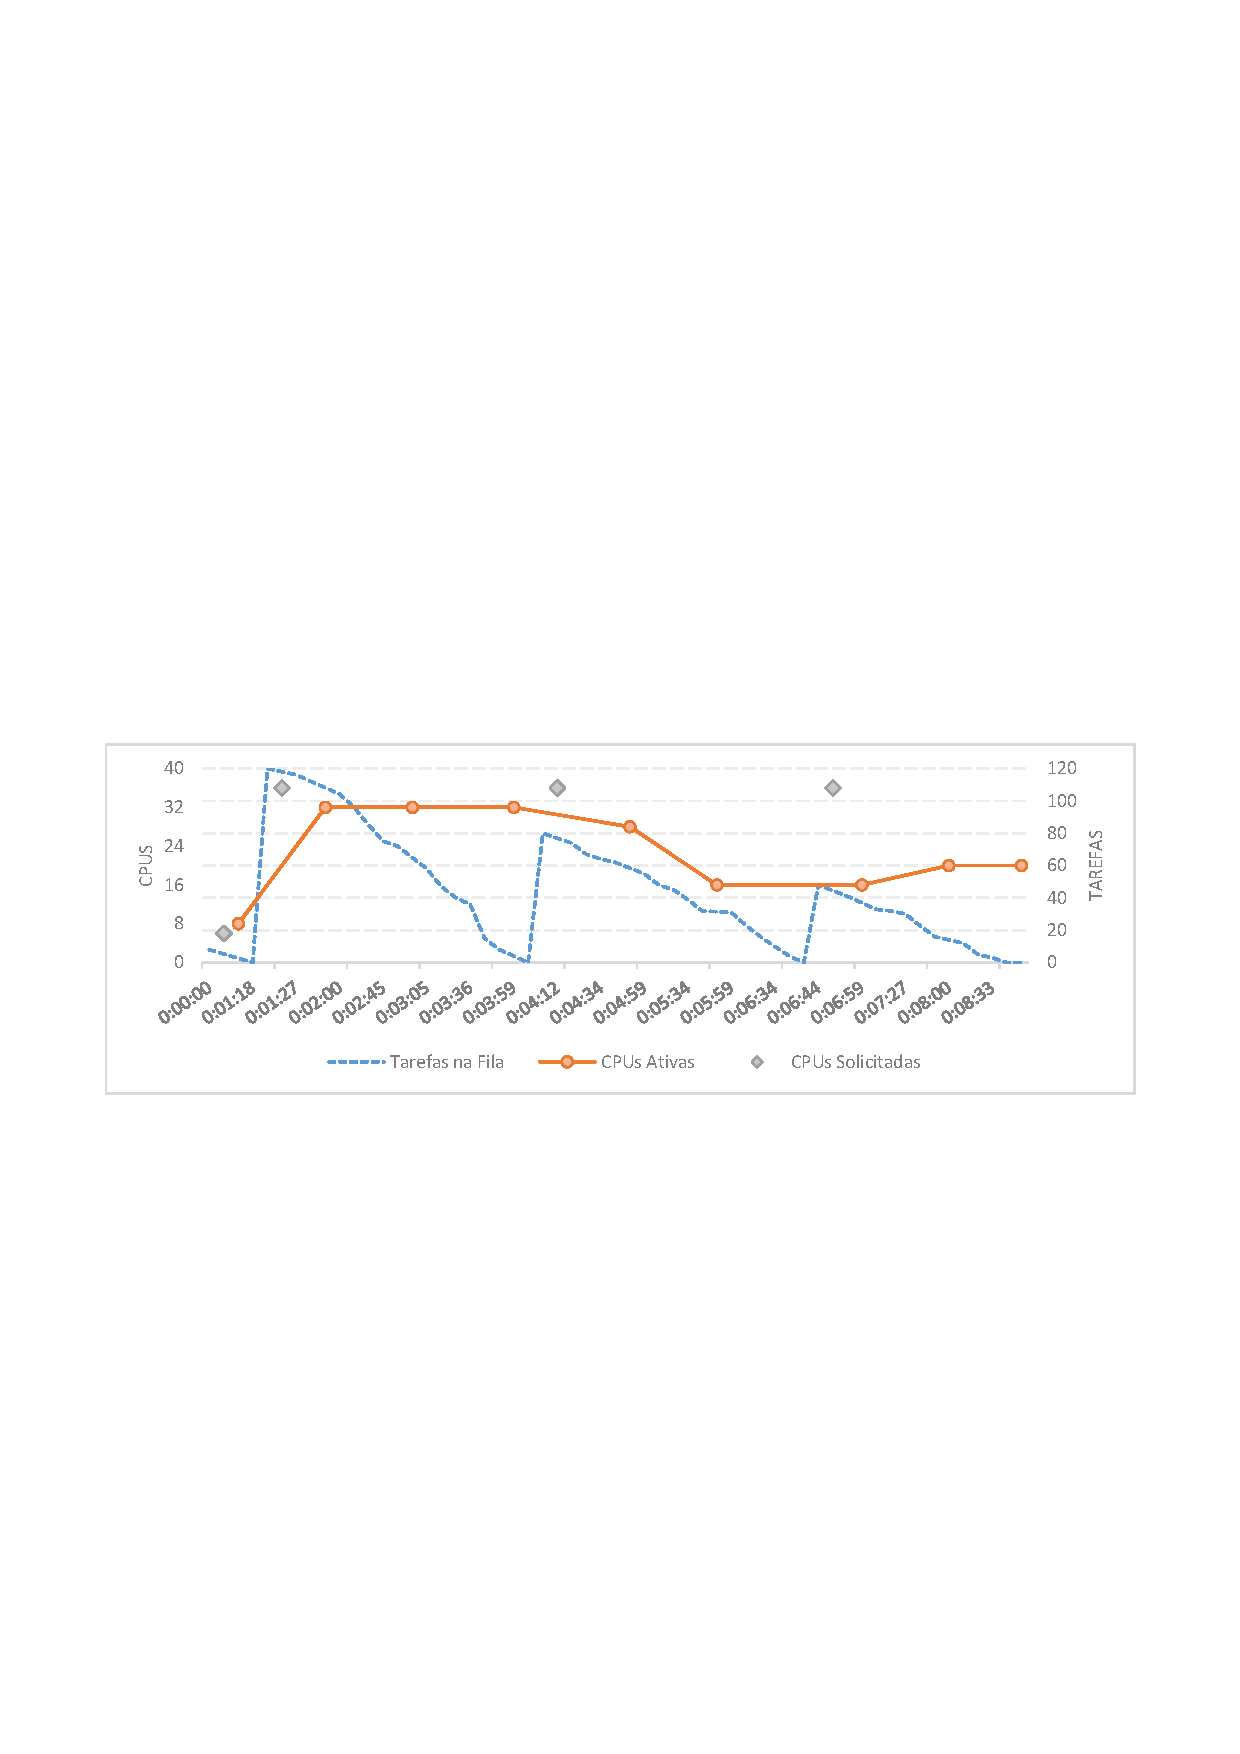
\includegraphics[trim=60 325 60 360,clip,width=\textwidth]{2018-12-16T05-17-35_rodents}
		\fonte{Elaborado pelo autor.}
	\end{minipage}
\end{figure}
\begin{figure}[p]
	\centering%
	\begin{minipage}{\textwidth}
		\caption{Comportamento de elasticidade para uma execução do arquivo 08-HIV\_vpu.ref2 no cenário $C_{c36}$.}
		\label{fig:results-modelo-batch-19HIV}
		\vspace{1ex}
		% esq | baixo | dir | alto
		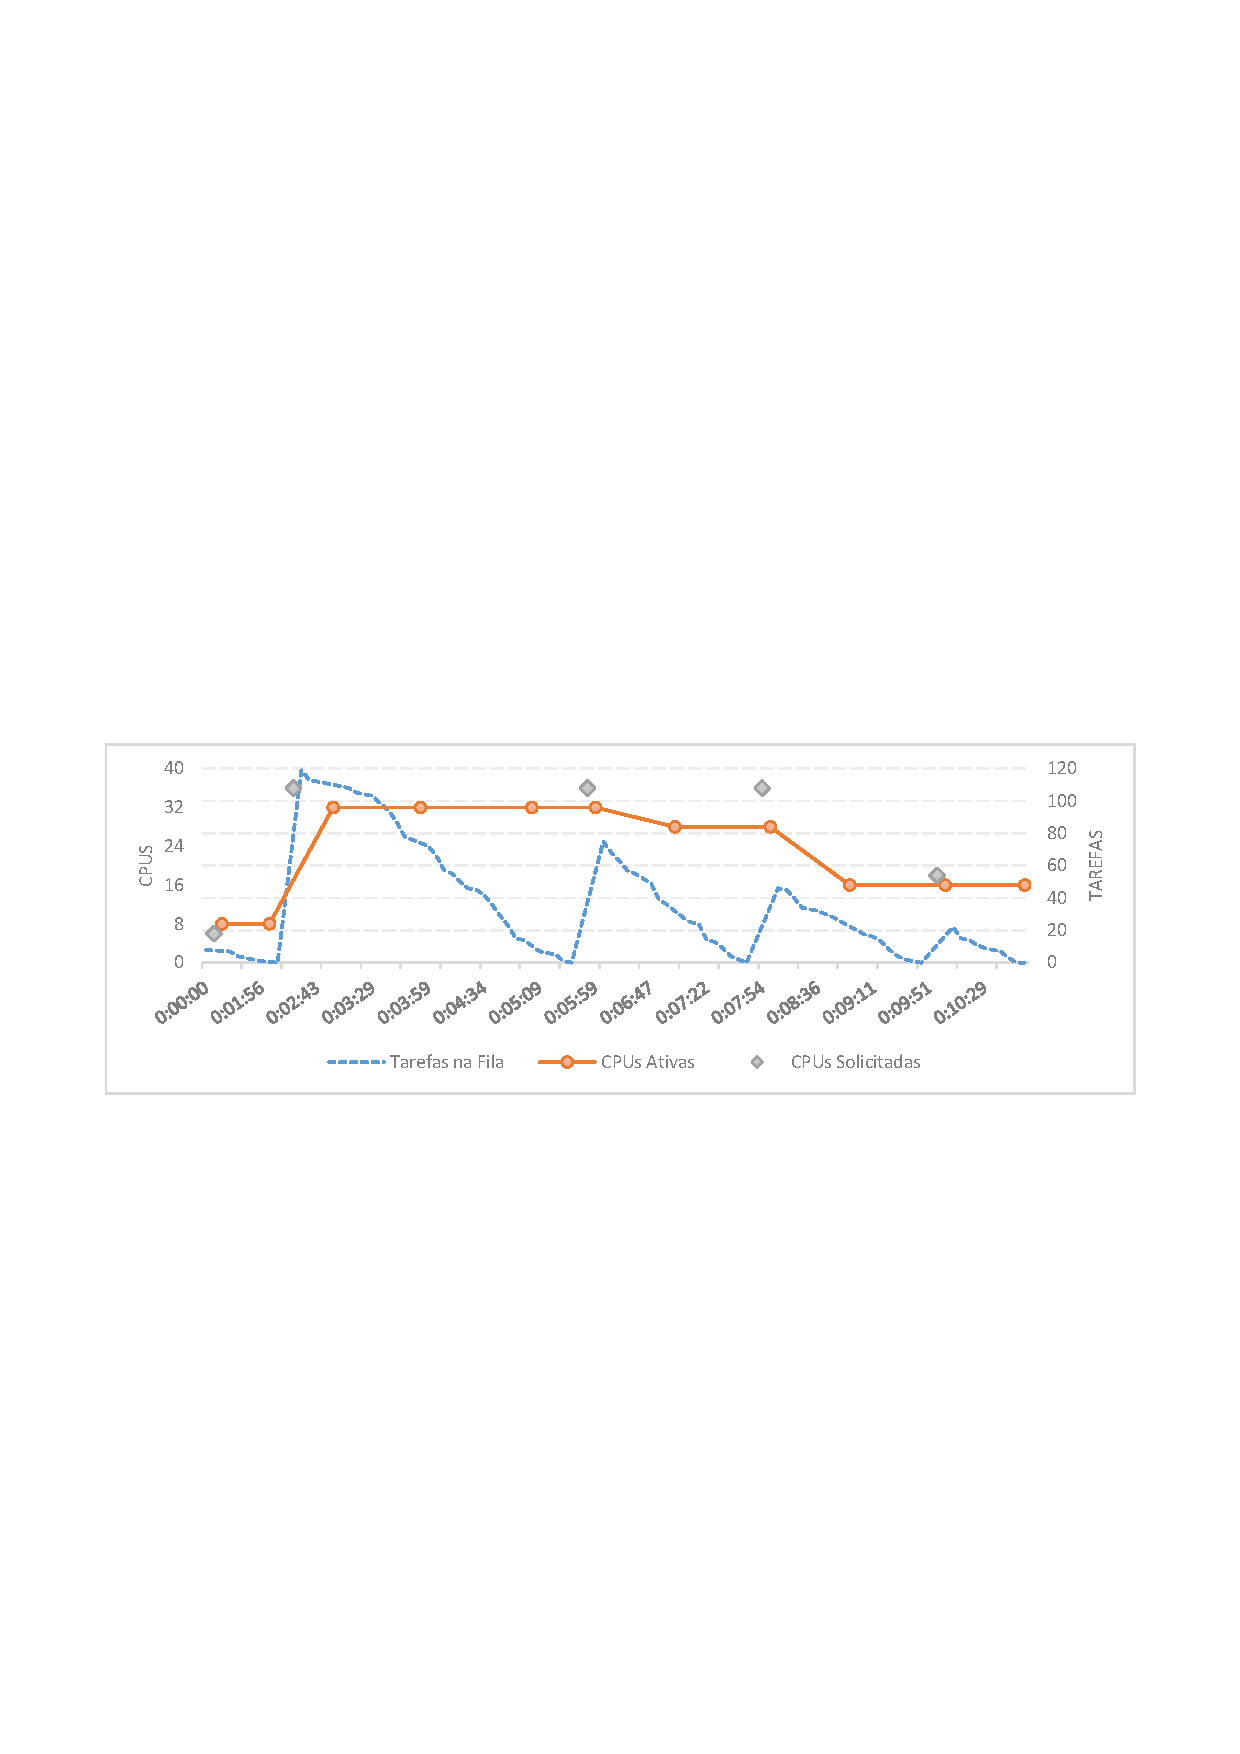
\includegraphics[trim=60 325 60 360,clip,width=\textwidth]{2018-12-16T11-19-00_HIV_vpu}
		\fonte{Elaborado pelo autor.}
	\end{minipage}
\end{figure}
\begin{figure}[p]
	\centering%
	\begin{minipage}{\textwidth}
		\caption{Comportamento de elasticidade contra--intuitivo para uma execução do arquivo 08-HIV\_vpu.ref2 no cenário $C_{c36}$.}
		\label{fig:results-modelo-batch-41HIV}
		\vspace{1ex}
		% esq | baixo | dir | alto
		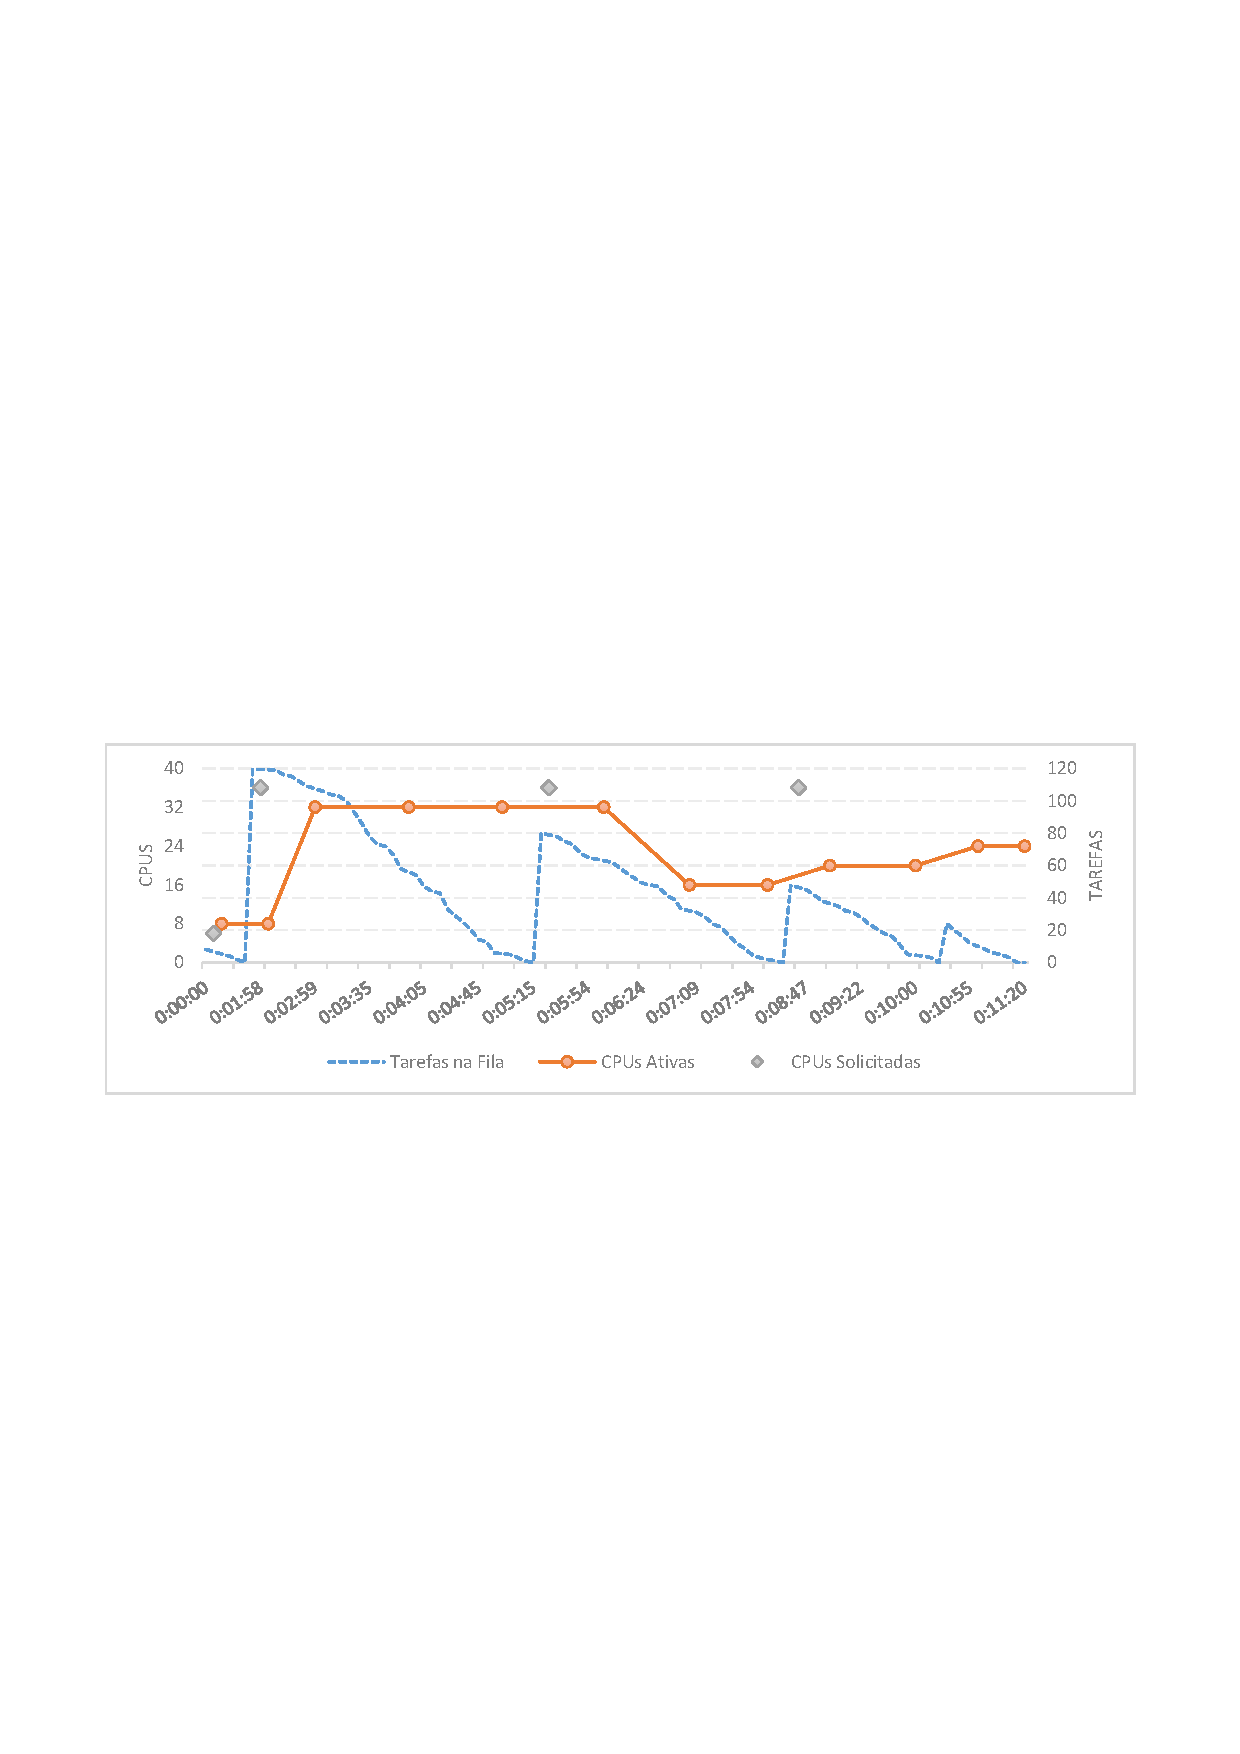
\includegraphics[trim=60 325 60 360,clip,width=\textwidth]{2018-12-16T11-41-09_HIV_vpu}
		\fonte{Elaborado pelo autor.}
	\end{minipage}
\end{figure}


No que tange ao comportamento de elasticidade da camada de Orquestração de Contêineres é possível inspecionar graficamente seu comportamento através de medições realizadas durante as execuções.
%
Os registros de monitoramento coletados pelo modelo \textsf{He}--lastic, assim como os dados do serviço CloudWatch do provedor de computação em nuvem AWS, permitem observar as ações tomadas pelo motor de elasticidade, ajudando a entender os motivos e as circunstâncias que causaram tais ações.


Como pode ser visto no conjunto de Figuras 
\ref{fig:results-modelo-batch-rodents}, 
\ref{fig:results-modelo-batch-19HIV},
\ref{fig:results-modelo-batch-41HIV},
\ref{fig:results-modelo-batch-primate},
\ref{fig:results-modelo-batch-stamatakis} e
\ref{fig:results-modelo-batch-stamatakis-detail},
o funcionamento do motor de elasticidade do serviço AWS Batch costuma seguir de maneira fiel, embora com algum atraso, a curva de demanda, exemplificado, por exemplo, na \autoref{fig:results-modelo-batch-rodents} e \autoref{fig:results-modelo-batch-19HIV}.
%
Estas duas imagens representam a visão geral do que foi observado pelo autor durante o acompanhamento da execução dos cenários de testes, onde geralmente o motor de elasticidade reage às variações na demanda com um \textit{delay} de até um ou dois minutos.
%
Os pontos demarcados com um losango representam ações preparatórias de elasticidade sugeridas pelo modelo \textsf{He}--lastic, conforme abordado na \autoref{sec:metodologia-prototipo-dificuldades} onde, por meio de chamadas de API é informado um número sugerido de CPUs a alocar para o processamento.
%
Contudo, como pode ser observado nas imagens, nem sempre o motor de elasticidade do serviço acata a estas sugestões, o que é considerado correto pelo autor uma vez que esta é apenas uma sugestão oriunda de uma heurística.


Como resultado da demanda em formato dente de serra, originada pela estratégia de \textit{Clustering Search} adotada pelo jModelTest, podem ocorrer instâncias de comportamento contra--intuitivo das ações de elasticidade, como exemplificado pela dupla de \autoref{fig:results-modelo-batch-41HIV} e \autoref{fig:results-modelo-batch-primate}.
%
Nestes casos existe uma retomada na quantidade de recursos alocados próximo ao final do processamento, geralmente originada por sugestão da heurística ou, na maioria dos casos, devido ao início de uma nova etapa de processamento que aumenta de maneira abrupta a quantidade de tarefas em espera na fila de processamento.
%
Como resultado deste repentino aumento nos recursos disponíveis, é possível observar um nível elevado de ociosidade nas VMs alocadas para atender estas requisições, um fenômeno que é agravado nos arquivos menores.



Em execuções do arquivo 01-aP6, por exemplo, é comum observar que o serviço Batch, responsável pela camada de Orquestração de Contêineres, tome mais tempo para distribuir as requisições entre as VMs disponíveis do que o tempo necessário para executar um dos cálculos de adequação dos sistemas de substituição molecular.
%
Este comportamento é oriundo do próprio serviço AWS Batch, de forma que não há parâmetro disponível para configurá-lo, e se manifesta através do aumento na ociosidade média dos recursos disponíveis, constituindo um cenário que deve ser evitado por seus usuários.
%
No caso do modelo \textsf{He}--lastic este fenômeno perde importância quando são utilizadas as duas camadas de elasticidade, haja vista que a camada FaaS irá absorver as tarefas mais curtas e evitar que este comportamento se manifeste.


\begin{figure}[p]
	\centering%
	\begin{minipage}{\textwidth}
		\caption{Comportamento de elasticidade contra--intuitivo para uma execução do arquivo 07-primate-mtDNA no cenário $C_{c36}$.}
		\label{fig:results-modelo-batch-primate}
		\vspace{1ex}
		% esq | baixo | dir | alto
		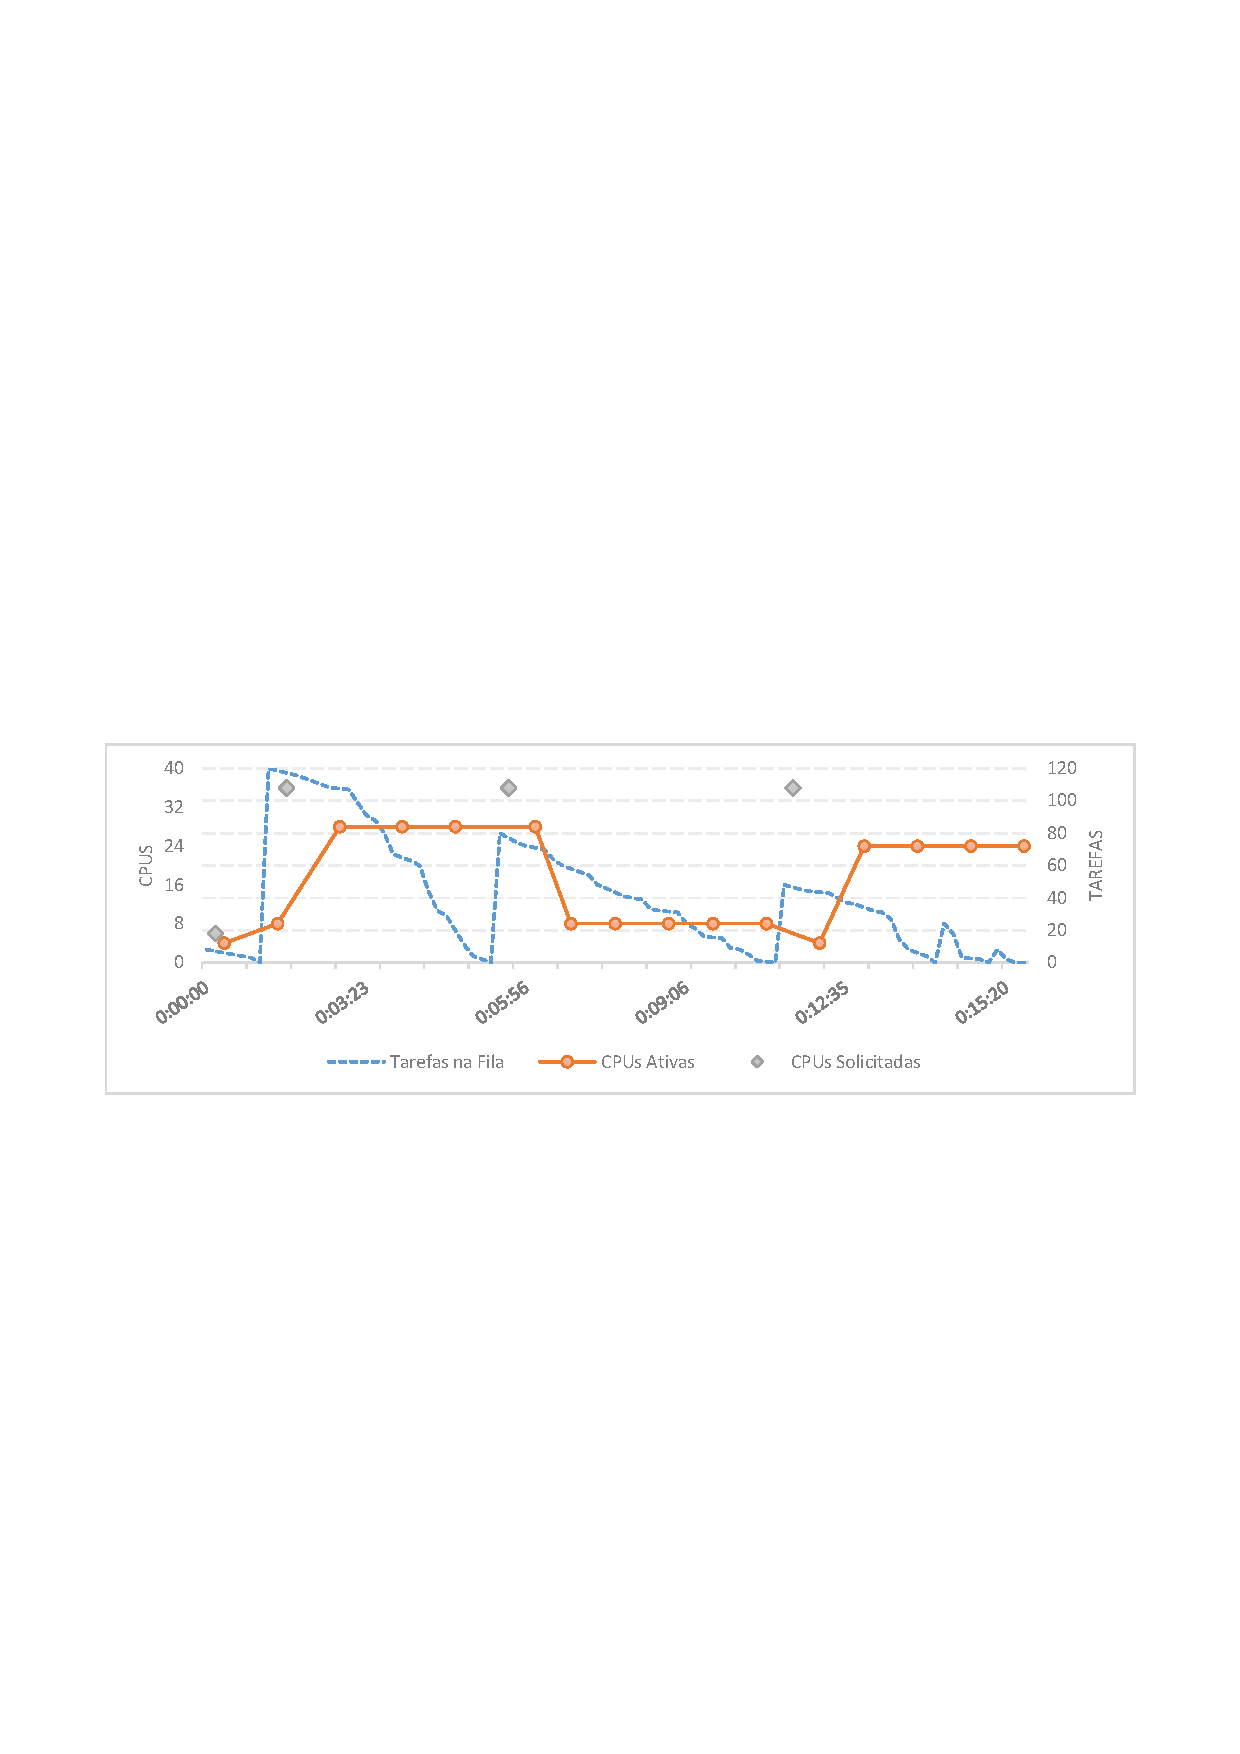
\includegraphics[trim=60 325 60 360,clip,width=\textwidth]{primate-mtDNA_36cpu}
		\fonte{Elaborado pelo autor.}
	\end{minipage}
\end{figure}
\begin{figure}[p]
	\centering%
	\begin{minipage}{\textwidth}
		\caption{Comportamento de elasticidade para uma execução do arquivo 12-stamatakis-59 no cenário $C_{c36}$.}
		\label{fig:results-modelo-batch-stamatakis}
		\vspace{1ex}
		% esq | baixo | dir | alto
		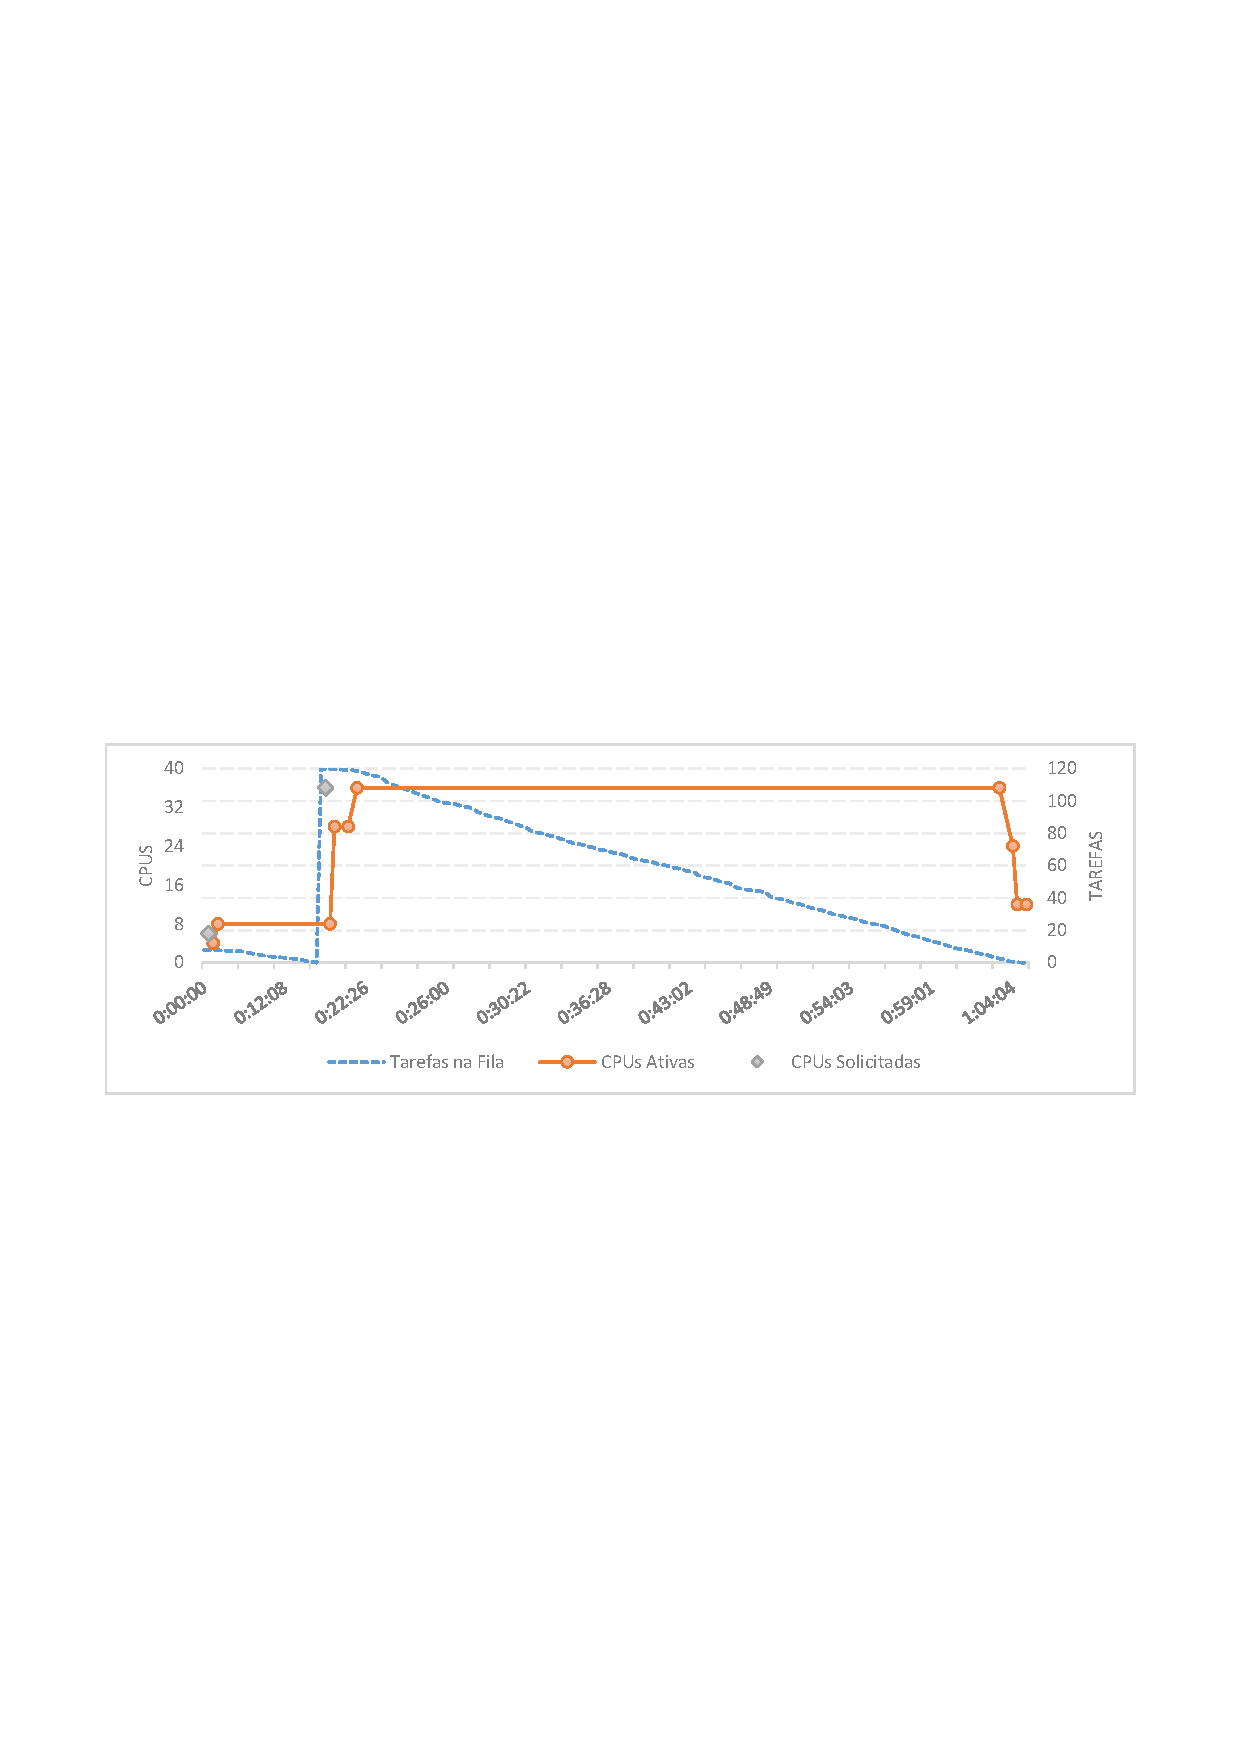
\includegraphics[trim=60 325 60 360,clip,width=\textwidth]{stamatakis_36cpu}
		\fonte{Elaborado pelo autor.}
	\end{minipage}
\end{figure}
\begin{figure}[p]
	\centering%
	\begin{minipage}{\textwidth}
		\caption{Percentual de uso de CPU para cada uma das VMs (com quatro \textit{cores} de processamento) ativas durante a execução do arquivo 12-stamatakis-59 no cenário $C_{c36}$.}
		\label{fig:results-modelo-batch-stamatakis-detail}
		\vspace{1ex}
		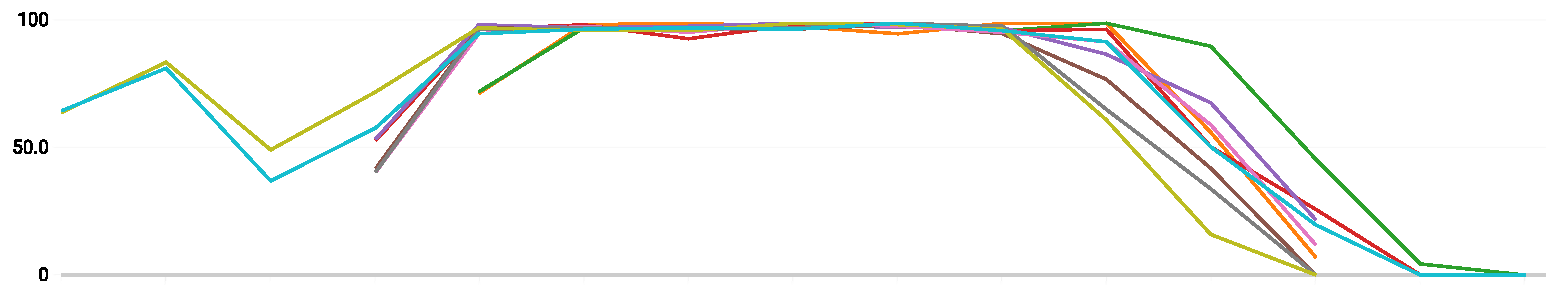
\includegraphics[width=\textwidth]{stamatakis_36cpu_processors}
		\fonte{Capturado pelo autor a partir do serviço CloudWatch do provedor AWS.}
	\end{minipage}
\end{figure}



Contudo, para afirmar com segurança que esta é uma característica do serviço utilizado como manipulador da camada de Orquestração de Contêineres ao invés de uma característica do modelo, seriam necessários mais cenários de testes com uma abordagem alternativa para o tratamento desta camada.
%
No entanto a experiência do autor sugere que este comportamento tem origem, de fato, na implementação interna do serviço AWS Batch.
%
Contudo, indiferente da origem deste comportamento, sua ocorrência perde relevância a medida que aumentam os tamanhos dos arquivos e as durações de cada requisição de processamento, reduzindo também seu impacto no desempenho do modelo \textsf{He}--lastic.


Por fim, as Figuras \ref{fig:results-modelo-batch-stamatakis} e
\ref{fig:results-modelo-batch-stamatakis-detail} tem por objetivo mostrar a progressividade das ações de elasticidade em um arquivo de maior duração, como o caso do 12-stamatakis-59.
%
Nesta execução, o gerenciador de elasticidade inicialmente lança mão de quatro \textit{cores} de processamento que, quase imediatamente, reconhece como insuficientes, dobrando a alocação para que cada uma das oito tarefas iniciais seja processada por um \textit{core} distinto.
%
Assim que se inicia a segunda etapa do processamento baseado em \textit{Clustering Search} mais uma ação de elasticidade é executada, trazendo o número de \textit{cores} disponível para 28 e, alguns minutos depois, para o teto configurado de 36.



Ao final do processamento, conforme vai aumentando a ociosidade das VMs alocadas o gestor de elasticidade inicia as reduções baixando para 24 \textit{cores} e, logo em seguida, para 12 \textit{cores} distribuídos em 3 VMs.
%
Por meio do monitoramento do arquivo 12-stamatakis-59 é possível perceber a relativa cautela com que o gerenciador de elasticidade executa suas ações, deixando um intervalo de tempo observado na casa dos cinco a dez minutos antes de efetivamente desligar uma VM.
%
Este comportamento pode ser explicado pela existência de alguma tarefa ainda em andamento em um dos \textit{cores} da VM, uma vez que o gerenciador só pode remover o recurso com segurança depois que todas as tarefas em execução na VM estejam concluídas.


Neste caso o gerenciador fica refém de tarefas atrasadas ou que recém foram alocadas, uma situação que se agrava conforme aumentam o número de \textit{cores} disponíveis na VM, o que aumenta também a probabilidade de haver tarefas ainda em andamento, apesar de boa parte da máquina estar ociosa.
%
O conservadorismo na hora de devolver recursos computacionais também pode ser explicado por uma possível política de redução de \textit{thrashing} adotada pelo serviço Batch, o que ajuda a reduzir o impacto de \textit{setup} de novos recursos.
%
Embora não haja menção oficial nas documentações a respeito de uma política de redução de \textit{thrashing}, é seguro assumir que um mecanismo análogo esteja em voga, pois é de interesse do usuário.







\subsection{Cenário Misto}

Já os cenários que contemplam a combinação entre as camadas de FaaS e Orquestração de Contêineres, representando a aplicação completa do modelo \textsf{He}--lastic, embora compartilhem a progressividade oriunda dos arquivos do \textit{dataset}, iniciam de patamar mais baixo que os demais e encerram com uma curva mais suave.
%
Neste caso os dados absolutos endossam os dados relativos, conciliando a \autoref{tab:results-modelo-avgs} com a \autoref{fig:results-modelo-caracteristicas}, uma validação que pode ser realizada através da comparação entre os menores e maiores arquivos do \textit{dataset}.
%
Assim é possível perceber que a estratégia empregada pelo modelo \textsf{He}--lastic é altamente eficaz quando processando em alta granularidade, ou seja, com pequenas tarefas individuais que, no caso desta avaliação, se manifestam por meio dos menores arquivos de alinhamentos de sequências moleculares.
%
No que diz respeito aos arquivos maiores, ou seja, unidades de processamento com menor granularidade, é possível observar uma degradação de performance quando comparados ao cenário que contempla apenas Orquestração de Contêineres, contudo os dados e o gráfico sugerem que este \textit{overhead} diminui conforme crescem os arquivos até eventualmente deixar de ser uma preocupação como pode ser observado no 12-stamatakis-59, o maior arquivo do \textit{dataset}.


\begin{table}[tb]
	\centering%
	\begin{minipage}{\defaultFigureWidth\textwidth}
		\caption{Razão dos sistemas de evolução processados pela camada de Orquestração de Contêineres sobre o total por arquivo e cenário observada na avaliação do \textsf{He}--lastic.}
		\label{tab:results-modelo-batchratio}
		\vspace{1ex}
		\begin{tabularx}{\textwidth}{@{\extracolsep{\fill}}lWWWWWWW@{}}
			\toprule
			& $C_{m1}$ & $C_{m2}$ & $C_{m3}$ & $C_{m4}$ & $C_{m5}$ & $C_{m6}$ & $C_{m7}$ \\
			\midrule
			08-HIV\_vpu.ref2 & --- & 1\% & --- & 48\% & 10\% & --- & 15\% \\
			09-gusanos16S.mafft & 21\% & 46\% & 20\% & 91\% & 53\% & 21\% & 51\% \\
			10-Birds & 2\% & 6\% & 2\% & 85\% & 43\% & 2\% & 46\% \\
			11-gusanosCOI.mafft & 51\% & 57\% & 50\% & 97\% & 78\% & 50\% & 77\% \\
			\bottomrule
			\multicolumn{1}{r}{Média Geral} & 26\% & 24\% & 24\% & 80\% & 46\% & 25\% & 47\% \\
		\end{tabularx}
		\tabelafootnote{{*}~São apresentados apenas os casos que satisfazem a condição $ 0\% < Raz\tilde{a}o < 100\% $.}
		\fonte{Elaborado pelo autor.}
	\end{minipage}
\end{table}



Uma observação mais próxima dos cenários mistos do modelo \textsf{He}--lastic ($C_{mX}$), ainda na \autoref{fig:results-modelo-caracteristicas}, mostra uma divergência de comportamento nos arquivos intermediários do \textit{dataset}, que podem ser reunidos em 2 grupos, contendo:
\begin{inparaenum}[\itshape a\upshape)] 
	\item os cenários que continuam apresentando um comportamento em linha com os cenários baseados em Orquestração de Contêineres (mais linear e progressivo); e
	\item os cenários que sofrem um impacto mais agressivo na performance, compostos por ($C_{m4}$, $C_{m5}$ e $C_{m7}$).
\end{inparaenum}
%
Para compreender este comportamento é necessário recorrer à \autoref{tab:results-modelo-batchratio} que apresenta a razão entre os sistemas de substituição molecular que foram processados pela camada de Orquestração de Contêineres sobre o total.



Assim, uma razão de 40\% indica que, do total de sistemas de substituição molecular testados para um determinado arquivo do \textit{dataset}, 60\% dos sistemas foram processados na camada FaaS e os 40\% restantes foram encaminhados para a segunda camada em função do limite no tempo de execução, sendo efetivamente processados pelo Orquestrador de Contêineres.
%
Através da média geral por cenário é possível perceber que os cenários $C_{m4}$, $C_{m5}$ e $C_{m7}$, que apresentaram um aumento mais agressivo no tempo de execução, são os que apresentam maior razão de sistemas processados na camada de Orquestração de Contêineres, com valores na faixa de 80\% para o cenário $C_{m4}$ e 45\% para os cenários $C_{m5}$ e $C_{m7}$.
Os demais cenários se mantém na faixa de 25\% dos sistemas processados pelo Orquestrador de Contêineres, resultando em uma curva mais suave conforme observado na \autoref{fig:results-modelo-caracteristicas}.



Por meio da análise conjunta sobre os dados da \autoref{tab:results-modelo-avgs}, \autoref{fig:results-modelo-caracteristicas} e \autoref{tab:results-modelo-batchratio} é possível estabelecer que a razão entre os arquivos processados pela camada FaaS e pela camada de Orquestração de Contêineres exerce uma significativa influência no tempo total das execuções quando se utiliza o modelo \textsf{He}--lastic.
%
Também é possível perceber, integrando na análise os dados da \autoref{tab:metodologia-cenarios-helastic}, que existe grande sensibilidade ao tempo limite de execução estabelecido para a camada FaaS, onde os arquivos processados pelos cenários $C_{m1}$, $C_{m3}$ e $C_{m6}$ apresentam os menores níveis de arquivos processados na camada de Orquestração de Contêineres.
%
Contudo, no que diz respeito ao tempo total de execução, a comparação entre os cenários $C_{m3}$ e $C_{m4}$ mostra que através da redução no tempo limite da camada FaaS para $1/4$ (de 60s para 15s), enquanto aumenta os recursos do Orquestrador de Contêineres em $2,25x$ (de 16 para 36), é possível obter melhores tempos de execução, conforme provam os resultados dos arquivos 09-gusanos16S.mafft, 11-gusanosCOI.mafft, e 12-stamatakis-59.



Estes dados sugerem a existência de um faixa do espaço de possíveis configurações do modelo \textsf{He}--lastic que necessita de uma escolha mais criteriosa para os seus valores, onde uma análise empírica pode ser uma aliada no ajuste fino destas configurações.
%
Embora não seja desejável na formulação de qualquer modelo, a aplicação de estratégias empíricas também é adotada por trabalhos como os de \citetexto{Shankar2018} e \citetexto{Jonas2017} devido à dificuldade em formalizar o comportamento dinâmico que se origina da combinação entre os parâmetros de Potência e Tempo Limite na camada FaaS sendo, no caso do modelo \textsf{He}--lastic, agravada pela existência de um terceiro fator, a Quantidade Limite de CPUs na camada de Orquestração de Contêineres.
%
A falta de modelos formais que sejam capazes de representar este comportamento dinâmico evidencia a necessidade de trabalhos futuros visando este objetivo, conclusão também obtida por \citetexto{Shankar2018}.


\afterpage{
	\clearpage
	\begin{landscape}
		\begin{table}
			\centering%
			\begin{minipage}{\linewidth}
				\caption{Diferenças nos tempos de execução entre os cenários de avaliação do modelo \textsf{He}--lastic com FaaS e Orquestração de Contêineres versus os cenários do jModelTest.}
				\label{tab:results-modelo-mixed}
				\vspace{0.75ex}
				\footnotesize
				%\small
				%\renewcommand\arraystretch{1.2}
		\begin{tabularx}{\linewidth}{@{\extracolsep{\fill}}lrrrrrrrrrrrrrr@{}}
			\toprule
			\multicolumn{1}{c}{\multirow{2}{*}{Arquivo}} & \multicolumn{2}{c}{$C_{m1}$} & \multicolumn{2}{c}{$C_{m2}$} & \multicolumn{2}{c}{$C_{m3}$} & \multicolumn{2}{c}{$C_{m4}$} & \multicolumn{2}{c}{$C_{m5}$} & \multicolumn{2}{c}{$C_{m6}$} & \multicolumn{2}{c}{$C_{m7}$} \\ 
			\cmidrule(r){2-3} 
			\cmidrule(lr){4-5} 
			\cmidrule(lr){6-7} 
			\cmidrule(lr){8-9} 
			\cmidrule(lr){10-11} 
			\cmidrule(lr){12-13} 
			\cmidrule(l){14-15} 
			& Razão & Delta & Razão & Delta & Razão & Delta & Razão & Delta & Razão & Delta & Razão & Delta & Razão & Delta \\
			\midrule
			01-aP6 & 81\% & -0:00:02 & 175\% & 0:00:05 & 188\% & 0:00:05 & 220\% & 0:00:05 & 221\% & 0:00:05 & 263\% & 0:00:07 & 297\% & 0:00:08 \\
			02-rodents & 22\% & -0:00:44 & 47\% & -0:00:15 & 49\% & -0:00:15 & 73\% & -0:00:05 & 73\% & -0:00:05 & 79\% & -0:00:04 & 126\% & 0:00:04 \\
			03-example & 30\% & -0:00:57 & 55\% & -0:00:20 & 58\% & -0:00:19 & 83\% & -0:00:04 & 92\% & -0:00:02 & 100\% & -0:00:00 & 163\% & 0:00:17 \\
			04-18S\_insects2 & 24\% & -0:01:03 & 41\% & -0:00:24 & 47\% & -0:00:22 & 77\% & -0:00:05 & 78\% & -0:00:05 & 89\% & -0:00:02 & 128\% & 0:00:06 \\
			05-HIVpol.groupM & 13\% & -0:03:06 & 25\% & -0:01:27 & 28\% & -0:01:23 & 41\% & -0:00:42 & 40\% & -0:00:42 & 45\% & -0:00:39 & 76\% & -0:00:17 \\
			06-Hex\_EF1a & 17\% & -0:04:46 & 32\% & -0:02:06 & 30\% & -0:02:09 & 55\% & -0:00:47 & 57\% & -0:00:44 & 58\% & -0:00:44 & 96\% & -0:00:04 \\
			07-primate-mtDNA & 23\% & -0:05:31 & 40\% & -0:02:26 & 39\% & -0:02:27 & 181\% & 0:02:07 & 59\% & -0:01:05 & 67\% & -0:00:52 & 105\% & 0:00:08 \\
			08-HIV\_vpu.ref2 & 35\% & -0:08:17 & 195\% & 0:06:22 & 67\% & -0:02:13 & 855\% & 0:29:15 & 878\% & 0:30:07 & 163\% & 0:02:25 & 1084\% & 0:38:06 \\
			09-gusanos16S.mafft & 151\% & 0:15:12 & 223\% & 0:19:25 & 237\% & 0:21:38 & 308\% & 0:21:35 & 322\% & 0:23:04 & 395\% & 0:30:39 & 362\% & 0:27:17 \\
			10-Birds & 38\% & -0:23:25 & 73\% & -0:05:39 & 71\% & -0:06:02 & 192\% & 0:11:30 & 189\% & 0:11:02 & 124\% & 0:02:57 & 220\% & 0:14:59 \\
			11-gusanosCOI.mafft & 160\% & 0:29:58 & 199\% & 0:27:11 & 212\% & 0:30:36 & 268\% & 0:27:21 & 297\% & 0:32:05 & 367\% & 0:43:24 & 356\% & 0:41:37 \\
			12-stamatakis-59 & 87\% & -0:33:38 & 76\% & -0:32:49 & 95\% & -0:06:46 & 90\% & -0:08:01 & 93\% & -0:06:06 & 99\% & -0:00:46 & 94\% & -0:04:53 \\ 
			\bottomrule
			\multicolumn{1}{r}{Média Geral} &  & \textcolor{success-green}{-0:02:50} &  & -0:00:26 &  & 0:02:21 &  & 0:06:03 &  & 0:07:25 &  & \textcolor{failure-red}{0:10:00} &  & 0:09:47 \\
			\multicolumn{1}{r}{Máxima} &  & 0:31:51 &  & \textcolor{success-green}{0:30:02} &  & 0:32:11 &  & 0:33:40 &  & 0:36:54 &  & \textcolor{failure-red}{0:52:25} &  & 0:42:50
		\end{tabularx}
		\fonte{Elaborado pelo autor.}
	\end{minipage}
\end{table}

\begin{figure}[p]
	\centering%
	\begin{minipage}{\linewidth}
		\caption{Mapa de calor da diferença percentual nos tempos de execução entre os cenários de avaliação do modelo \textsf{He}--lastic com FaaS e Orquestração de Contêineres versus os cenários do jModelTest.}
		\label{fig:results-modelo-mixed}
		\vspace{1ex}
		% esq | baixo | dir | alto
		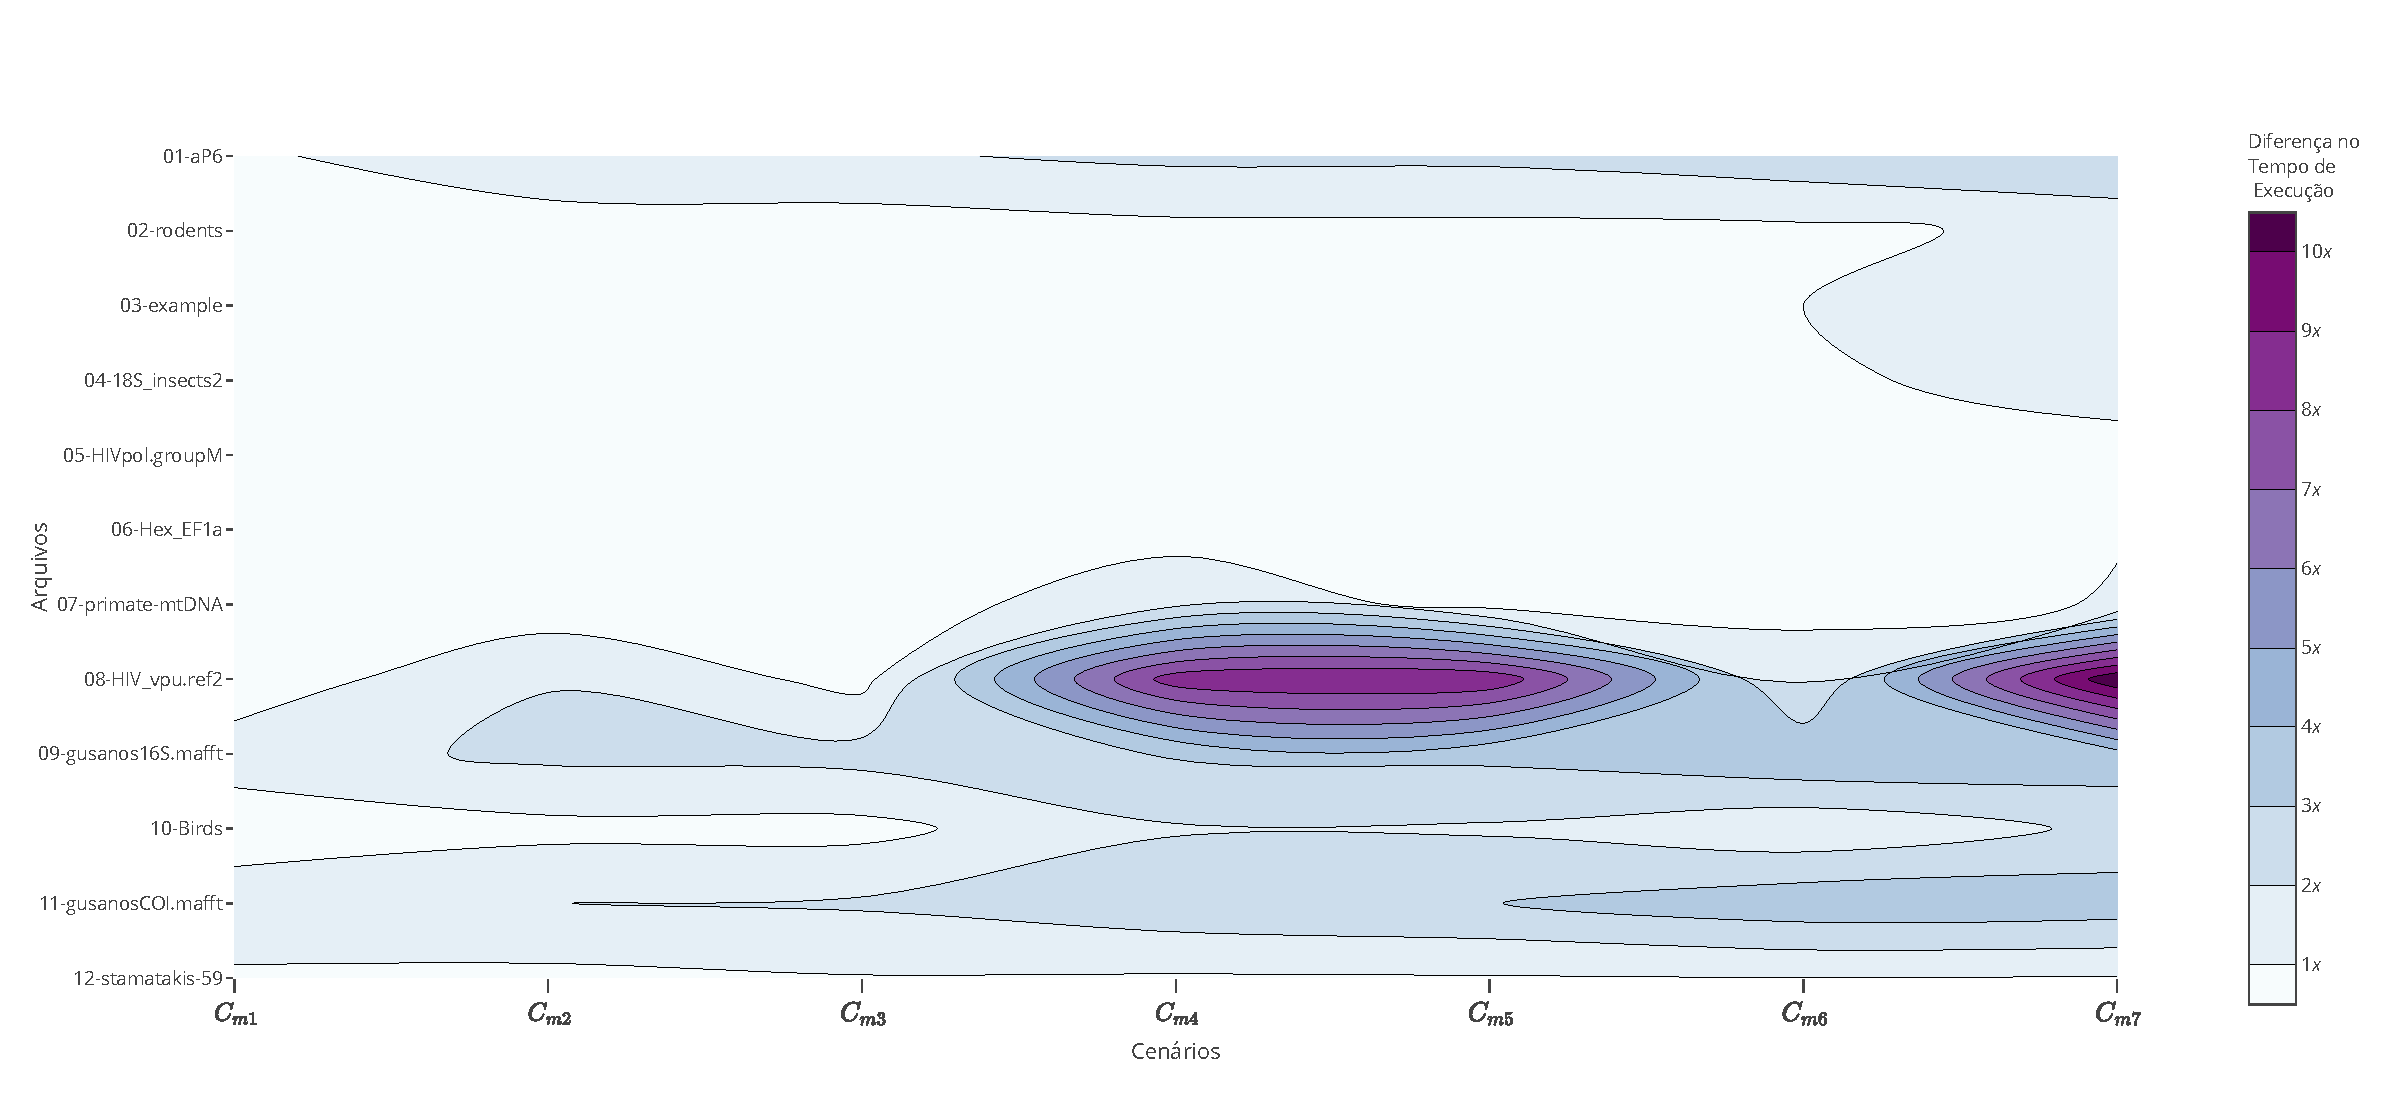
\includegraphics[trim=0 38 0 70,clip,width=\textwidth]{results-modelo-mixed}
		\fonte{Elaborado pelo autor.}
	\end{minipage}
\end{figure}

\end{landscape}
}


Como estratégia para avaliar o grau de \textit{overhead} gerado pelo modelo \textsf{He}--lastic sobre a execução do software jModelTest, uma medida de variação no tempo de execução foi adotada, comparando os tempos médios das execuções por arquivo dos cenários $C_{mX}$ versus os cenários $C_{jX}$ com a mesma quantidade de CPUs.
%
Desta forma, o cenário $C_{m1}$ é comparado com $C_{j8}$, os cenários $C_{m2}$ e $C_{m3}$ são comparados com $C_{j16}$ e os demais cenários são comparados com $C_{j36}$, como pode ser visto pela análise das Tabelas \ref{tab:metodologia-cenarios-jmodel} e \ref{tab:metodologia-cenarios-helastic}.
%
Embora a comparação por meio da quantidade de CPUs seja intuitiva, ela se mostra incompleta uma vez que, do lado do jModelTest a quantidade de CPUs mapeia a disponibilidade destes recursos ao longo da execução, enquanto no modelo \textsf{He}--lastic ela mapeia a quantidade máxima do recurso que pode ou não ser alocado conforme o comportamento de elasticidade.
%
Além disso, não é possível estabelecer um paralelo entre as duas abordagens comparadas no que diz respeito à alocação de recursos da camada FaaS, haja vista que não há nenhuma semelhança entre os conceitos de Potência e Tempo Limite de execução, parâmetros fundamentais para o modelo \textsf{He}--lastic e a camada FaaS.
%
Contudo, mesmo que a comparação dos cenários por meio do número de CPUs não seja ideal, ela apresenta--se como a alternativa mais próxima para uma comparação justa entre as abordagens do modelo \textsf{He}--lastic e do jModelTest.



Por meio dos dados apresentados na \autoref{tab:results-modelo-mixed} é possível perceber que, na maioria dos arquivos do \textit{dataset} de testes, a abordagem do modelo \textsf{He}--lastic se mostra favorável quando avaliada em termos do tempo total de execução.
%
Observando as diferenças nos tempos de execução ao longo de todos os cenários avaliados é possível perceber que os maiores ganhos estão concentrados nos arquivos de tamanho pequeno a intermediários do \textit{dataset}, com destaque para os arquivos 05-HIVpol.groupM e 06-Hex\_EF1a, onde foi possível obter tempos de execução que levaram menos de 25\% do tempo dos cenários base do jModelTest.
%
O arquivo 01-aP6 pode ser incluído nesta classificação pois, embora sua variação percentual seja significativa, ela não apresenta grande relevância quando avaliada em termos absolutos, devido ao pequeno tamanho do arquivo e consequente curta duração de processamento.


Nos arquivos considerados maiores os resultados são de interpretação mais complexa, uma vez que existe um claro ganho de performance, embora pequeno, no caso do arquivo 12-stamatakis-59, que não é compartilhado com os arquivos.
%
A região que contempla os arquivos do intervalo 07 à 11 merece especial atenção devido aos resultados mistos obtidos, conforme o cenário executado.
%
Chamam a atenção nesta análise os resultados obtidos pelo arquivo 08-HIV\_vpu.ref2 nos cenários $C_{m7}$, $C_{m5}$ e $C_{m4}$, com variações percentuais de 1084\%, 878\% e 855\%, respectivamente.


Para auxiliar na compreensão destes resultados a \autoref{fig:results-modelo-mixed} apresenta um mapa de calor que abrange os dados da \autoref{tab:results-modelo-mixed}, possibilitando a análise visual dos resultados obtidos.
%
Com a ajuda desta figura é possível perceber que os resultados do arquivo 08-HIV\_vpu.ref2 são localizados, afetando de maneira mais grave apenas este arquivo nos cenários previamente mencionados.
%
Nos demais arquivos e cenários a variação observada se concentra na faixa entre 100\% à 400\%, o que, embora não seja encorajador, não causa o mesmo nível de espanto dos valores observados para o arquivo 08.


Uma nova análise da \autoref{tab:results-modelo-batchratio} resulta em uma forte correlação com a \autoref{fig:results-modelo-mixed}, fornecendo uma explicação para o formato da região que sofreu maior impacto de performance em função da adoção do modelo \textsf{He}--lastic.
%
Embora nem todos os arquivos e cenários apresentem correlação tão intensa quanto o 10-Birds, por exemplo, a \autoref{tab:results-modelo-batchratio} fornece um importante \textit{insight} sobre o motivo desta degradação de performance, nomeadamente a taxa de requisições que foram atendidas pela segunda camada do modelo.
%
No caso do protótipo que toma por base a implementação do jModelTest, isto se traduz na razão dos sistemas de substituição molecular cujo cálculo não foi possível de realizar na camada FaaS, necessitando a transição para a camada de Orquestração de Contêineres.
%
Uma ressalva importante na análise da \autoref{tab:results-modelo-batchratio} deve ser feita quanto ao arquivo 12-stamatakis-59 que, embora não conste na tabela, tem a totalidade de suas requisições, ou seja, 100\%, atendidas pela camada de Orquestração de Contêineres e, por consequência, sofrendo o mesmo tipo de \textit{overhead} que os demais arquivos e cenários.


Como já previamente abordado na \autoref{sec:metodologia-prototipo-dificuldades}, uma das grandes dificuldades encontradas na avaliação do protótipo se deu em função da incapacidade de influenciar a quantidade de \textit{retries} realizados pela camada FaaS quando uma requisição ultrapassa o tempo limite de execução.
%
Especula-se que os \textit{retries} impostos pelo serviço Lambda do provedor AWS estejam contribuindo de maneira significativa para o impacto de performance observado.
%
A proporcionalidade do tempo de espera entre os \textit{retries}, que segue a política de \textit{backoff} exponencial, também é visível nos dados da \autoref{tab:results-modelo-mixed}, onde o cenário $C_{m7}$ que tem \textit{timeout} configurado de 60 segundos é que apresenta maior impacto de performance, seguido dos cenários $C_{m5}$ e $C_{m4}$, com \textit{timeouts} de 30 e 15 segundos, respectivamente.



Outro fator que gera impacto é o \textit{overhead} oriundo da camada de Orquestração de Contêineres, que se mostrou, de acordo com resultados prévios, mais conservador nas ações de elasticidade, até mesmo deixando de utilizar na totalidade os recursos disponibilizados.
%
Assim como observado no cenário de avaliação baseado somente em Orquestração de Contêineres, por meio das Figuras \ref{fig:results-modelo-batch-rodents}, \ref{fig:results-modelo-batch-19HIV}, \ref{fig:results-modelo-batch-41HIV} e \ref{fig:results-modelo-batch-primate}, nos cenários de avaliação do modelo \textsf{He}--lastic com suas duas camadas é recorrente o comportamento conservador na alocação de recursos por parte do gerenciador de elasticidade.
%
Nestes casos, mesmo que os parâmetros do modelo permitam utilizar até 36 \textit{cores} de processamento, como no cenário $C_{m3}$ por exemplo, o gestor de elasticidade do serviço AWS Batch aloca em torno de 20 para efetuar a execução, o que causa um efeito negativo no tempo de execução, embora positivo do ponto de vista do custo.
%
Mesmo que seja possível justificar este comportamento, que pode ser adotado para mitigar a ocorrência de \textit{thrashing} de recursos, nos cenários de processamento compartilhado entre as duas camadas do modelo \textsf{He}--lastic há um perceptível impacto no desempenho em termos do tempo de processamento, como pode ser observado na \autoref{fig:results-modelo-mixed}.




Há, ainda, o agravante da estratégia de \textit{Clustering Search} adotada pelo jModelTest, que faz com que os impactos sejam ainda mais agudos quando o \textit{overhead} da camada de Orquestração de Contêineres inicia próximo do final de uma etapa, o que faz com que todas as demais etapas fiquem represadas até que as últimas requisições sejam atendidas.
%
Ilustra este cenário uma situação onde o último dos sistemas de substituição molecular a ser avaliado em uma etapa do processamento excede os limites da camada FaaS e deve, portanto, ser encaminhado para o Orquestrador de Contêineres, o que faz com que todo o restante do processamento deva necessariamente esperar pela conclusão deste último atrasado, podendo, inclusive, causar um efeito bola de neve caso a situação se repita nas próximas etapas.




Todavia é relevante ponderar também sobre os resultados obtidos pelo arquivo 12-stamatakis-59 que obteve até mesmos ganhos marginais de performance ao longo de todos os cenários de avaliação mesmo enfrentando todos os \textit{delays} e dificuldades mencionadas acima.
%
Neste arquivo, nem o impacto dos \textit{retries} impostos pelo serviço AWS Lambda, nem o impacto da elasticidade do serviço AWS Batch foram capazes de se traduzir em degradação de performance quando avaliado sob o critério do tempo de execução.
%
Assim é possível concluir que tais \textit{overheads} se tornam cada vez menos relevantes conforme cresce o tamanho do arquivo (e o tamanho do grão de elasticidade).
%
Embora o conjunto de arquivos de teste não contemple arquivos maiores do que este, o autor considera seguro assumir que este comportamento representa uma tendência, embora haja carência de evidências.




Também carece investigação os resultados encontrados no que tange ao arquivo 08-HIV\_vpu.ref2 em busca de uma conclusão autoritativa acerca do alto impacto de performance encontrado no seu processamento.
%
Como já mencionado anteriormente, parte da resposta pode ser atribuída à necessidade de processar uma parcela das requisições na camada de Orquestração de Contêineres.
%
Contudo este argumento não é capaz de explicar o nível tão elevado de \textit{overhead} quando comparado aos demais arquivos que também tiveram parte das requisições atendidas pela segunda camada do modelo \textsf{He}--lastic.
%
Uma segundo fator pode estar associado à quantidade de etapas de processamento que o arquivo é submetido na estratégia de \textit{Clustering Search} do jModelTest, onde o 08-HIV\_vpu.ref2, conforme dados das Tabelas \ref{tab:modelo-elasticidade-jmodelsteps} e \ref{tab:metodologia-etapas-dataset} é submetido à cinco etapas de processamento devido aos seus 280 sistemas de substituição
%
Dentre os arquivos que passam pela camada de Orquestrador de contêineres, o 08-HIV\_vpu.ref2 é o que contempla maior número de etapas, conforme mostra o levantamento a seguir: 
\begin{inparaenum}[] 
	\item 08-HIV\_vpu.ref2: 5 etapas;
	\item 09-gusanos16S.mafft: 4 etapas;
	\item 10-Birds: 3 etapas;
	\item 11-gusanosCOI.mafft: 4 etapas; e
	\item 12-stamatakis-59: 2 etapas.
\end{inparaenum}



\begin{table}[tb]
\centering%
\begin{minipage}{\defaultFigureWidth\textwidth}
	\caption{Consolidação dos resultados obtidos nas execuções dos cenários mistos do modelo \textsf{He}--lastic em comparação com os resultados das execuções do jModelTest.}
	\label{tab:results-modelo-mixed-summary}
	\vspace{1ex}
	\begin{tabular*}{\linewidth}{@{\extracolsep{\fill}}crcrrr@{}}
		\toprule
		\multicolumn{2}{c}{Cenário de Referência} & \multicolumn{2}{c}{Cenário \textsf{He}--lastic} & 
		\multicolumn{2}{c}{Diferença} \\ 
		\cmidrule(r){1-2}
		\cmidrule(lr){3-4}
		\cmidrule(l){5-6}
		Código & \begin{tabular}[c]{@{}r@{}}Duração\\ Média\end{tabular} & Código & \begin{tabular}[c]{@{}r@{}}Duração\\ Média\end{tabular} & Média & Percentual \\ 
		\midrule
		$C_{j8}$ & 0:32:01 & $C_{m1}$ & 0:31:08 & \textcolor{success-green}{-0:00:53} & -3\% \\ 
		\dashedline{1-6}
		\multirow{2}{*}{$C_{j16}$} & \multirow{2}{*}{0:17:31} & $C_{m2}$ & 0:15:46 & \textcolor{success-green}{-0:01:45} & -10\% \\
		&  & $C_{m3}$ & 0:19:36 & 0:02:05 & 12\% \\ 
		\dashedline{1-6}
		\multirow{4}{*}{$C_{j36}$} & \multirow{4}{*}{0:10:33} & $C_{m4}$ & 0:15:45 & \textcolor{success-green}{0:05:12} & 49\% \\
		&  & $C_{m5}$ & 0:18:43 & 0:08:10 & 77\% \\
		&  & $C_{m6}$ & 0:26:41 & 0:16:08 & 153\% \\
		&  & $C_{m7}$ & 0:20:54 & 0:10:21 & 98\% \\ 
		\bottomrule
	\end{tabular*}
	\fonte{Elaborado pelo autor.}
\end{minipage}
\end{table}


 



Por fim, retornando aos resultados da \autoref{tab:results-modelo-mixed}, foram destacadas duas métricas referentes às diferenças nos tempos de execução, sendo uma delas a média geral, que agrupa todos os dados coletados em termos das suas diferenças nos tempos de execução e fornece um indicador totalizado para o tempo de execução de cada cenário.
Assim como a máxima, que demonstra o maior tempo de execução observado dentre todos os dados que compõem os resultados do cenário.
%
Por meio destas duas métricas é possível determinar um dos cenários como o melhor, de acordo com os critérios do usuário ou o ambiente onde será utilizado o modelo \textsf{He}--lastic.
%
Por exemplo, em um ambiente caracterizado por alto volume de requisições paralelas e usuários concorrendo por recursos, pode se mais apropriado adotar uma estratégia que busque minimizar o tempo máximo de espera, reduzindo o efeito conhecido como cauda longa.
%
Para este caso o melhor cenário seria o $C_{m2}$, embora seguido de perto pelos cenários $C_{m1}$, $C_{m3}$ e $C_{m4}$, com a pior escolha, segundo este critério, sendo o cenário $C_{m6}$.




Contudo, de maneira geral, é possível estabelecer o cenário $C_{m1}$ como o melhor dentre os cenários que fazem uso das duas camadas de elasticidade do modelo \textsf{He}--lastic, onde este apresenta um desempenho levemente superior ao cenário de referência do jModelTest com 8 CPUs disponíveis, $C_{f8}$.
%
Observando os cenários que disponibilizam 16 CPUs para o jModelTest é possível elencar o $C_{m2}$ como o melhor deles, novamente apresentando resultado em linha com os tempos de execução observados no cenário de referência.
%
Por fim, no comparativo com os cenários que poderiam fazer uso de até 36 CPUs no jModelTest, o cenário $C_{m4}$ é escolhido como o mais apropriado, resultando, infelizmente, em uma ineficiência média frente ao cenário base $C_{f36}$ de seis minutos.



Os resultados gerais podem ser visualizados na \autoref{tab:results-modelo-mixed-summary} que apresenta, por meio das médias dos tempos de execução, o panorama comparativo entre as execuções do modelo \textsf{He}--lastic com suas duas camadas de elasticidade versus as execuções do jModelTest.
%
A escolha das médias, embora possa parecer contra--intuitiva, foi necessária em função da diferença na quantidade de execuções por arquivo e cenário, sendo utilizada neste contexto como meio para obter uma comparação justa entre as duas abordagens.
%
Desta forma, em termos do tempo médio de execução por arquivo, é possível estabelecer que a abordagem do modelo proposto é vantajosa quando comparada a execuções do jModelTest com recursos fixos de 8 e 16 CPUs, conforme dados dos cenários $C_{j8}$ e $C_{j16}$.
%
Contudo, este resultado não se sustenta quando os recursos disponíveis para o jModelTest são aumentados para 36 CPUs no cenário $C_{j36}$, onde há uma perda de eficiência da abordagem com elasticidade, representada pelo modelo proposto, frente a abordagem de recursos fixos do jModelTest.




%\begin{verbatim}
%	warm04-60-768-36
%		falar que esse cenário foi um tira-teima pra ver se o tempo a mais era em função das operações de elasticidade ou dos retries
%		warm04		=	 investigate wether the increased runtime is due to scaling actions or retries
%\end{verbatim}








\section{Avaliação de Custos}



Uma vez compreendido o comportamento do modelo \textsf{He}--lastic no que diz respeito a performance medida pelo tempo de execução, o presente trabalho prossegue para a análise de custo.
%
Todos os dados apresentados aqui tem como base as métricas de avaliação estabelecidas na \autoref{sec:modelo-metricas}, contudo, para fins de apresentação, somente serão demonstrados os valores de custo Financeiro, uma vez que esta é a única métrica capaz de harmonizar os custos do modelo de alocação de recursos fixos, do jModelTest puro, da camada FaaS e da camada de Orquestração de Contêineres utilizadas pelo modelo proposto.



Adicionalmente, os cenários utilizados para comparação de custos foram reduzidos para somente os que contemplam a execução do modelo \textsf{He}--lastic na sua abordagem mista, ou seja, com ambas as camadas de elasticidade habilitadas.
%
Os identificadores de tais cenários seguem o formato $C_{mX}$ e foram escolhidos para esta análise aqueles que apresentaram melhor desempenho em termos dos tempos de execução conforme a quantidade de recursos disponível para alocação.
%
Como já discutido, embora a quantidade de recursos não seja um indicativo confiável de semelhança entre os cenários, ele se mostrou o único viável na comparação entre jModelTest e o modelo proposto.


O critério de seleção dos cenários que participam da análise comparativa de custos se baseou nos dados das Tabelas \ref{tab:results-modelo-mixed} e \ref{tab:results-modelo-mixed-summary}, escolhendo o que obteve melhor desempenho quando agrupados em termos da quantidade de CPUs disponíveis para alocação, conforme determinado na definição dos cenários de avaliação para o modelo \textsf{He}--lastic na \autoref{tab:metodologia-cenarios-helastic}.
%
Como resultado, obtêm-se os cenários $C_{m1}$, $C_{m2}$ e $C_{m4}$ como participantes da análise de custos.
%
Não foram selecionados para esta etapa de análise os cenários dedicados a uma única das camadas de elasticidade pois a intenção é avaliar de maneira consolidada as características de desempenho, seja em termos do tempo de execução ou de custo financeiro, do modelo proposto.
%
Além disso, no caso do cenário somente FaaS ($C_{f0}$), não seria possível obter um resultado conclusivo, haja vista que a camada FaaS é incapaz de processar todos os arquivos contidos no \textit{dataset} em função dos limites estabelecidos pelo próprio modelo computacional.



São apresentados na \autoref{tab:results-custos-modelo} os principais indicadores que afetam na determinação do custo financeiro para os cenários do modelo \textsf{He}--lastic, onde, além dos cenários selecionados para análise, foram incluídos os cenários exclusivos de avaliação de uma das camadas de elasticidade para referência.
%
Todos os valores do corpo da tabela são sumarizados através das suas médias, com a exceção dos dados totalizados que realizam o somatório dos dados de duração e custo financeiro.
%
O indicador de CPUs, presente na tabela, representa, em contraste com o parâmetro de configuração do modelo, a quantidade efetiva de unidades de processamento utilizadas durante a avaliação da dupla arquivo--cenário.



\afterpage{
	\clearpage
	\begin{landscape}
		\begin{table}
			\centering%
			\begin{minipage}{\linewidth}
				\caption{Resultados médios das avaliações de performance e custo financeiro dos cenários do modelo \textsf{He}--lastic por arquivo do \textit{dataset}.}
				\label{tab:results-custos-modelo}
				\vspace{0.75ex}
				%\scriptsize
				\footnotesize
				%\small
				\renewcommand\arraystretch{1.4}
				\begin{tabular*}{\linewidth}{@{\extracolsep{\fill}}lrrrrrrrrrrrrrrrrrr@{}}
					\toprule
					\multicolumn{1}{c}{\multirow{2}{*}{Arquivo}} & \multicolumn{3}{c}{$C_{f0}$} & \multicolumn{3}{c}{$C_{c36}$} & \multicolumn{4}{c}{$C_{m1}$} & \multicolumn{4}{c}{$C_{m2}$} & \multicolumn{4}{c}{$C_{m4}$} \\
					\cmidrule(r){2-4}
					\cmidrule(lr){5-7}
					\cmidrule(lr){8-11}
					\cmidrule(lr){12-15}
					\cmidrule(l){16-19}
					\multicolumn{1}{c}{} &
					\rotatebox[origin=c]{\tabelaAngulo}{Duração} & \rotatebox[origin=c]{\tabelaAngulo}{CPUs} & \rotatebox[origin=c]{\tabelaAngulo}{Financeiro} &
					\rotatebox[origin=c]{\tabelaAngulo}{Duração} & \rotatebox[origin=c]{\tabelaAngulo}{CPUs} & \rotatebox[origin=c]{\tabelaAngulo}{Financeiro} & 
					\rotatebox[origin=c]{\tabelaAngulo}{Duração} & \rotatebox[origin=c]{\tabelaAngulo}{CPUs} & \rotatebox[origin=c]{\tabelaAngulo}{Razão} &  \rotatebox[origin=c]{\tabelaAngulo}{Financeiro} &
					\rotatebox[origin=c]{\tabelaAngulo}{Duração} & \rotatebox[origin=c]{\tabelaAngulo}{CPUs} & \rotatebox[origin=c]{\tabelaAngulo}{Razão} &  \rotatebox[origin=c]{\tabelaAngulo}{Financeiro} &
					\rotatebox[origin=c]{\tabelaAngulo}{Duração} & \rotatebox[origin=c]{\tabelaAngulo}{CPUs} & \rotatebox[origin=c]{\tabelaAngulo}{Razão} & \rotatebox[origin=c]{\tabelaAngulo}{Financeiro}
					\\
					\midrule
					01-aP6 & 0:00:09 & 63 & 0,000 & 0:10:02 & 21 & 0,240 & 0:00:09 & 70 & 0\% & 0,000 & 0:00:11 & 29 & 0\% & 0,000 & 0:00:09 & 78 & 0\% & 0,000 \\
					02-rodents & 0:00:13 & 114 & 0,010 & 0:09:06 & 20 & 0,190 & 0:00:13 & 113 & 0\% & 0,010 & 0:00:14 & 88 & 0\% & 0,007 & 0:00:13 & 121 & 0\% & 0,008 \\
					03-example & 0:00:27 & 118 & 0,010 & 0:10:14 & 21 & 0,236 & 0:00:24 & 115 & 0\% & 0,010 & 0:00:25 & 114 & 0\% & 0,011 & 0:00:22 & 114 & 0\% & 0,010 \\
					04-18S\_insects2 & 0:00:19 & 117 & 0,010 & 0:09:23 & 20 & 0,159 & 0:00:20 & 102 & 0\% & 0,010 & 0:00:17 & 118 & 0\% & 0,010 & 0:00:17 & 116 & 0\% & 0,010 \\
					05-HIVpol.grou{[}..{]} & 0:00:30 & 120 & 0,020 & 0:08:55 & 22 & 0,208 & 0:00:28 & 120 & 0\% & 0,020 & 0:00:28 & 120 & 0\% & 0,020 & 0:00:29 & 120 & 0\% & 0,020 \\
					06-Hex\_EF1a & 0:00:59 & 120 & 0,030 & 0:08:28 & 23 & 0,172 & 0:00:59 & 119 & 0\% & 0,032 & 0:00:59 & 120 & 0\% & 0,036 & 0:00:57 & 120 & 0\% & 0,030 \\
					07-primate-mtDNA & 0:01:37 & 120 & 0,050 & 0:10:51 & 21 & 0,255 & 0:01:36 & 120 & 0\% & 0,050 & 0:01:35 & 121 & 0\% & 0,050 & 0:04:44 & 121 & 0\% & 0,052 \\
					08-HIV\_vpu.ref2 & 0:04:41 & 122 & 0,150 & 0:11:18 & 23 & 0,324 & 0:04:31 & 120 & 0\% & 0,153 & 0:13:01 & 144 & 1\% & 0,185 & 0:32:45 & 156 & 48\% & 0,454 \\
					09-gusanos16S{[}..{]} &  &  &  & 0:13:17 & 28 & 0,388 & 0:44:12 & 166 & 21\% & 0,546 & 0:35:21 & 190 & 46\% & 0,540 & 0:32:28 & 174 & 91\% & 0,581 \\
					10-Birds &  &  &  & 0:09:15 & 23 & 0,242 & 0:14:31 & 144 & 2\% & 0,218 & 0:15:28 & 145 & 6\% & 0,254 & 0:23:19 & 147 & 85\% & 0,578 \\
					11-gusanosCOI{[}..{]} &  &  &  & 0:19:58 & 25 & 0,460 & 1:18:26 & 200 & 51\% & 0,840 & 0:54:39 & 174 & 57\% & 0,796 & 0:43:13 & 166 & 97\% & 0,785 \\
					12-stamatakis-59 &  &  &  & 1:05:33 & 26 & 1,346 & 3:41:16 & 135 & 100\% & 1,385 & 1:47:52 & 142 & 100\% & 1,411 & 1:15:33 & 153 & 100\% & 1,456 \\
					\bottomrule
					\multicolumn{1}{r}{Total\textsuperscript{\dag}} & 0:08:55 & 112 & 0,28 & 3:06:21 & 23 & 4,22 & 6:07:05 & 127 & 14\% & 3,27 & 3:50:29 & 125 & 18\% & 3,32 & 3:34:29 & 132 & 35\% & 3,99
				\end{tabular*}
				\tabelafootnote{\textsuperscript{\dag}~Na linha de totais as informações são apresentadas da seguinte forma: Duração e Financeiro = Soma, CPUs e Razão = Média.}
				\fonte{Elaborado pelo autor.}
			\end{minipage}
		\end{table}
		
		
		
		
		\begin{table}
			\centering%
			\begin{minipage}{\linewidth}
				\caption{Resultados médios das avaliações de performance e custo financeiro dos cenários do jModelTest por arquivo do \textit{dataset}..}
				\label{tab:results-custos-jmodeltest}
				\vspace{0.75ex}
				%\scriptsize
				%\footnotesize
				%\small
				\renewcommand\arraystretch{1.4}
				\begin{tabular*}{\linewidth}{@{\extracolsep{\fill}}lrrrrrrrrrr@{}}
					\toprule
					\multicolumn{1}{c}{\multirow{2}{*}{Arquivo}} & \multicolumn{2}{c}{$C_{j2}$} & \multicolumn{2}{c}{$C_{j4}$} & \multicolumn{2}{c}{$C_{j8}$} & \multicolumn{2}{c}{$C_{j16}$} & \multicolumn{2}{c}{$C_{j36}$} \\
					\cmidrule(r){2-3}
					\cmidrule(lr){4-5}
					\cmidrule(lr){6-7}
					\cmidrule(lr){8-9}
					\cmidrule(l){10-11}
					\multicolumn{1}{c}{} & Duração & Financeiro & Duração & Financeiro & Duração & Financeiro & Duração & Financeiro & Duração & Financeiro \\
					\midrule
					01-aP6 & 0:00:40 & 0,0010 & 0:00:21 & 0,0010 & 0:00:11 & 0,0010 & 0:00:06 & 0,0012 & 0:00:04 & 0,0018 \\
					02-rodents & 0:03:20 & 0,0047 & 0:01:41 & 0,0048 & 0:00:57 & 0,0054 & 0:00:29 & 0,0055 & 0:00:17 & 0,0074 \\
					03-example & 0:04:42 & 0,0067 & 0:02:23 & 0,0068 & 0:01:22 & 0,0077 & 0:00:45 & 0,0085 & 0:00:27 & 0,0113 \\
					04-18S\_insects2 & 0:04:52 & 0,0069 & 0:02:27 & 0,0069 & 0:01:23 & 0,0078 & 0:00:41 & 0,0078 & 0:00:22 & 0,0095 \\
					05-HIVpol.groupM & 0:11:58 & 0,0170 & 0:06:10 & 0,0175 & 0:03:34 & 0,0202 & 0:01:55 & 0,0217 & 0:01:11 & 0,0302 \\
					06-Hex\_EF1a & 0:20:12 & 0,0286 & 0:10:16 & 0,0291 & 0:05:45 & 0,0326 & 0:03:05 & 0,0350 & 0:01:44 & 0,0444 \\
					07-primate-mtDNA & 0:24:23 & 0,0345 & 0:12:26 & 0,0352 & 0:07:07 & 0,0403 & 0:04:01 & 0,0455 & 0:02:37 & 0,0666 \\
					08-HIV\_vpu.ref2 & 0:45:38 & 0,0647 & 0:22:56 & 0,0650 & 0:12:39 & 0,0717 & 0:06:41 & 0,0757 & 0:03:52 & 0,0987 \\
					09-gusanos16S.mafft & 1:44:52 & 0,1486 & 0:53:06 & 0,1504 & 0:29:46 & 0,1687 & 0:15:47 & 0,1788 & 0:10:24 & 0,2651 \\
					10-Birds & 2:11:50 & 0,1868 & 1:07:34 & 0,1914 & 0:37:38 & 0,2133 & 0:20:53 & 0,2366 & 0:12:28 & 0,3179 \\
					11-gusanosCOI.mafft & 2:58:49 & 0,2533 & 1:31:03 & 0,2580 & 0:50:14 & 0,2847 & 0:27:22 & 0,3101 & 0:16:15 & 0,4145 \\
					12-stamatakis-59 & 14:51:54 & 1,2635 & 7:30:39 & 1,2768 & 4:15:20 & 1,4469 & 2:19:30 & 1,5811 & 1:23:34 & 2,1310 \\
					\bottomrule
					\multicolumn{1}{r}{Total} & 23:43:11 & 2,02 & 12:01:01 & 2,04 & 6:45:56 & 2,30 & 3:41:15 & 2,51 & 2:13:16 & 3,40
				\end{tabular*}
				%\tabelafootnote{{*}~Na linha de totais as informações são apresentadas da seguinte forma: Duração e Financeiro = Soma, CPUs e Razão = Média.}
				\fonte{Elaborado pelo autor.}
			\end{minipage}
		\end{table}
	\end{landscape}
}



O termo CPU, neste caso, adquire um sentido mais amplo, contemplando tanto o conceito clássico de \textit{cores} de um microprocessador, quanto os contêineres ou unidades de processamento da camada FaaS, o que explica a grande quantidade reportada na tabela.
%
Desta forma, as 127 CPUs utilizadas em média no cenário $C_{m4}$ correspondem a um valor $ CPU = CPU_{faas} + CPU_{conteineres} $, onde a quantidade de CPUs utilizadas na camada de Orquestração de Contêineres é um valor inteiro compreendido no intervalo $ 0 \le x \le CPU_{max} $, sendo o limite superior o valor do parâmetro do modelo.




% baixa utilização de CPUs pelo gerenciador de elasticidade do Batch

Ainda no que diz respeito a CPUs utilizadas é possível confirmar o fenômeno mencionado na \autoref{sec:resultados-modelo-faas}, onde o número de Processos / CPUs tende a se aproximar do nível máximo de paralelismo estabelecido pelo mecanismo de \textit{Clustering Search} adotado pelo jModelTest.
%
Contudo, ainda mais interessante é a análise do cenário $C_{c36}$, correspondente ao modelo \textsf{He}--lastic utilizando apenas a camada de Orquestração de Contêineres, que apresenta mais uma evidência a respeito do comportamento conservador do gerenciador de elasticidade do serviço AWS Batch, utilizado pela camada.
%
Mesmo configurado para utilizar até 36 \textit{cores} de processamento, o gerenciador de elasticidade adota, neste cenário, um comportamento bastante conservador ao alocar menos de cinco CPUs para os arquivos 04-18S\_insects2 e 12-stamatakis-59, o que representa menos de 15\% do valor permitido.
%
Embora este comportamento não seja nocivo para o custo financeiro, uma vez que este acompanha a quantidade de recursos utilizados no tempo, a baixa alocação efetiva traz impactos perceptíveis na duração do processamento, e provavelmente está ocorrendo também nos demais cenários, embora mascarado pela grande quantidade de CPUs da camada FaaS.



Por fim, ainda no contexto da \autoref{tab:results-custos-modelo}, as colunas denominadas Razão apresentam os mesmos dados contidos na \autoref{tab:results-modelo-batchratio}, ilustrando a divisão de tarefas entre as camadas do modelo \textsf{He}--lastic.
%
Assim como nos casos anteriores, esta razão representa a quantidade de sistemas de substituição molecular, ou as tarefas individuais, que foram processadas pela camada de Orquestração de Contêineres sobre o total das tarefas executadas no processamento de cada arquivo do \textit{dataset}.
%
No contexto da \autoref{tab:results-custos-modelo} sua presença é relevante para observar o impacto, tanto a nível de custo quanto a nível de tempo de execução, causado pela transição entre camadas.
%
Os arquivos 08-HIV\_vpu.ref2 e 09-gusanos16S.mafft no cenário $C_{m1}$ ilustram bem esta situação, onde um aumento na razão para aproximadamente 20\%, faz com que o custo financeiro passe de \$ 0,153 para \$ 0,546.
%
Como comparação, esta mesma transição avaliada no cenário composto apenas pelo Orquestrador de Contêineres ($C_{c36}$), passa de \$ 0,324 para \$ 0,388, resultando em um aumento no custo de apenas 16\%, em linha com o respectivo aumento no tempo de execução, enquanto na ocorrência de transição entre camadas de elasticidade, o aumento observado no custo é maior que 70\% e acompanhado de um aumento de 90\% no tempo de execução.



Estes resultados mostram que a ineficiência observada durante a transição entre camadas, em função de fatores previamente mencionados como o obrigatoriedade de \textit{retries} imposto pelo serviço AWS Lambda, assim como possíveis ineficiências ou políticas subjacentes opacas na gestão de elasticidade adotada pelo serviço AWS Batch, é um grave ponto de atenção para o modelo \textsf{He}--lastic.
%
O mapa de calor dos tempos de execução, apresentado na \autoref{fig:results-modelo-mixed}, volta a ser relevante aqui para caracterizar este fenômeno como centrado nos pontos de transição entre camadas.
%
No caso das execuções que apresentam uma baixa razão de transição entre camadas, assim como aqueles que nem precisariam passar pela primeira camada, como o caso dos arquivos maiores como o 12-stamatakis-59, o nível de impacto causado pela adoção do modelo proposto é negligenciável.
%
Assim, o resultado final desta análise, evidencia a necessidade de trabalhos futuros para investigar os motivos deste \textit{overhead}, assim como o investimento na concepção de técnicas e métodos capazes de mitigar este impacto.




Os resultados da análise dos custos associados a execução do programa jModelTest, nos cenários de avaliação estabelecidos na \autoref{sec:metodologia-etapasecenarios}, pode ser visto na \autoref{tab:results-custos-jmodeltest}, onde constam os resultados médios de tempo de execução e custo financeiro para as duplas arquivo--cenário, assim como os totalizadores por cenário.
%
Um ponto de fundamental atenção é que os resultados ali apresentados contemplam apenas os custos incorridos durante o tempo de execução dos cenários, sendo definitivamente otimistas uma vez que o projeto jModelTest, devido à sua ausência de diretivas de elasticidade, necessita de um servidor ou \textit{cluster} computacional disponível para atender as solicitações de processamento.
%
Contudo, sua análise permanece relevante ao estabelecer uma referência de eficiência máxima para os resultados do modelo \textsf{He}--lastic, onde é adotada a suposição de que os cenários do jModelTest sejam capazes de funcionar com recursos intermitentes, como é o caso do modelo proposto.


Assim como nas análises do tempo de execução, fica visível nos resultados da  \autoref{tab:results-custos-jmodeltest} a perda de eficiência do jModelTest conforme aumentam os recursos.
%
Esta perda é atribuída ao método de \textit{Clustering Search} adotado pela aplicação, que divide em etapas o processamento dos sistemas de substituição molecular, fazendo com que haja ociosidade significativa no final de cada etapa conforme aumentam os recursos disponíveis para execução dos cálculos, que são, por natureza, embaraçosamente paralelos.
%
Tal perda também se manifesta na forma de custo financeiro uma vez que, no formato tradicional de alocação de recursos em nuvem, a cobrança se dá pelo tempo que uma VM foi utilizada, desconsiderando o nível de utilização da mesma.



Seguindo esta lógica, se o comportamento de escalabilidade do programa jModelTest fosse próximo de linear, o custo observado deveria se manter praticamente constante, uma vez que o aumento nos recursos é compensado, em mesma proporção, pela redução no tempo de execução.
%
É possível verificar indícios deste comportamento ótimo de escalabilidade na evolução dos primeiros cenários de teste, onde $C_{j2}$, $C_{j4}$ e $C_{j8}$ apresentam leves aumentos, que são considerados normais para um programa com boas características de elasticidade.
%
No entanto, a medida que segue aumentando a quantidade de recursos disponíveis, neste caso a CPU por conta da natureza \textit{CPU--bound} do cálculo, tanto o tempo de execução quanto o custo se descolam de uma linha reta e passam a assumir um comportamento que lembra mais uma função polinomial.
%
Assim, o resultado de custo \$ 3,40 para o cenário $C_{j36}$, representa uma ineficiência de quase 70\% sobre o custo esperado de \$ 2,02 caso o programa apresentasse comportamento linear de escalabilidade, reconhecidamente uma tarefa difícil mas possível devido a natureza embaraçosamente paralela do processamento realizado.




Consolidando os resultados obtidos para os cenários de avalição do jModelTest e do modelo \textsf{He}--lastic, a \autoref{tab:results-custos-summary} apresenta o comparativo dos desempenhos em termos de tempo de execução e custos dos dados coletados.
%
Estão representados, na tabela, os cenários de teste do jModelTest com seus custos mínimos, calculados estritamente em função do tempo de execução, assim como os dados dos cenários com melhor desempenho em termos dos tempos de execução obtidos para o modelo proposto.
%
A comparação entre eles foi realizada através do cálculo do percentual que cada uma das métricas representa sobre a soma dos resultados obtidos pelo cenário do jModelTest e o do \textsf{He}--lastic, onde um resultado de 50\% representa o equilíbrio entre as abordagens, consequência de tempos de execução e/ou custos iguais.
%
Adicionalmente, os resultados da tabela são agrupados por número de CPUs alocadas em cada cenário, sendo esta a característica que chega mais próxima de estabelecer um nível de comparação, conforme mencionado anteriormente.



\begin{table}[tb]
	\centering%
	\begin{minipage}{\defaultFigureWidth\textwidth}
		\caption{Consolidação dos resultados obtidos dentre os cenários selecionados do modelo \textsf{He}--lastic e seus cenários análogos no jModelTest.}
		\label{tab:results-custos-summary}
		\vspace{1ex}
		\begin{tabular*}{\linewidth}{@{\extracolsep{\fill}}ccrrrrc@{}}
			%\cmidrule(lr){3-4}
			%\cmidrule(lr){5-6}
			%\dashedline{1-7}
			\toprule
			\multirow{2}{*}{\begin{tabular}[c]{@{}c@{}}CPUs\\ Alocadas\end{tabular}} & \multicolumn{1}{c}{\multirow{2}{*}{Cenário}} & \multicolumn{2}{c}{Totais} & \multicolumn{2}{c}{Percentual} & \multicolumn{1}{c}{\multirow{2}{*}{\begin{tabular}[c]{@{}c@{}}Ineficiência\\ \textsf{He}--lastic\end{tabular}}} \\
			\cmidrule(lr){3-4}
			\cmidrule(lr){5-6}
			& & Duração & Custo & Duração & Custo & \\
			\midrule
			\multirow{2}{*}{8} & $C_{m1}$ & 6:07:31 & 3,27 & 48\% & 59\% & \multirow{2}{*}{6\%} \\
			& $C_{j8}$ & 6:45:56 & 2,30 & 52\% & 41\% &  \\
			\dashedline{1-7}
			\multirow{2}{*}{16} & $C_{m2}$ & 3:50:29 & 3,32 & 51\% & 57\% & \multirow{2}{*}{8\%} \\
			& $C_{j16}$ & 3:41:15 & 2,51 & 49\% & 43\% &  \\
			\dashedline{1-7}
			\multirow{2}{*}{36} & $C_{m4}$ & 3:34:29 & 3,99 & 62\% & 54\% & \multirow{2}{*}{16\%} \\
			& $C_{j36}$ & 2:13:16 & 3,40 & 38\% & 46\% & \\
			\bottomrule
		\end{tabular*}
		\fonte{Elaborado pelo autor.}
	\end{minipage}
\end{table}



Por fim, na última coluna da \autoref{tab:results-custos-summary}, é apresentada uma métrica que representa a soma das variações sobre o valor ideal de 50\% para cada uma das características avaliadas, representando o resultado geral do comparativo entre os cenários contrapostos.
%
Sua análise fornece um critério final de escolha, capaz de determinar a melhor relação custo--benefício em termos da redução de custo financeiro e tempo total de execução.
%
Chamada de Ineficiência \textsf{He}--lastic, a métrica é calculada através da fórmula $ VarPctg(\text{Duração}) + VarPctg(\text{Custo}) - 1 $, representando, portanto, uma visão agregada das características de desempenho avaliadas onde ambas compartilham o mesmo nível de importância para o valor final.




Desta maneira é possível perceber que o modelo proposto apresenta, de maneira geral um impacto de performance, ou seja, uma perda de eficiência sobre a abordagem base do jModelTest, no intervalo de aproximadamente 5\% à 15\% dentre todos os cenários contemplados na avaliação.
%
Também é possível identificar que as perdas acompanham o crescimento da quantidade de recursos disponível em termos do número de CPUs alocados para uso, lembrando que devido às duas camadas de elasticidade empregadas no modelo o verdadeiro valor acaba variando conforme as características do processamento e as configurações adotadas.


% cenário 8 cpu

Os resultados demonstram que, na comparação entre os cenários que contemplam o uso de até oito CPUs, há um impacto da ordem de 6\% na adoção do modelo \textsf{He}--lastic, traduzindo em um número as conclusões obtidas no que diz respeito à duração e custo, onde foi possível atingir uma redução da duração de 2\% sobre a abordagem do jModelTest enquanto utilizaram-se quase 10\% mais recursos na forma de custo financeiro.
%
Embora a redução na duração pareça pequena em termos percentuais, ela se traduz numa economia de quase 40 minutos (0:38:25) sobre as quase sete horas de execução contabilizadas na abordagem do jModelTest.
%
Contudo, a contrapartida de custos para este ganho de 2\% no tempo de execução, se manifesta na forma de um custo 9\% maior, saindo de \$ 2,30 na abordagem do jModelTest, para \$ 3,27 quando há adoção do modelo \textsf{He}--lastic parametrizado conforme o cenário de testes $C_{m1}$.



% cenário 16 cpu

No comparativo entre os cenários que alocam até 16 CPUs o quadro se agrava no que diz respeito à perda de eficiência, com o índice subindo para 8\%.
%
Esta perda é resultado da variação marginal no tempo de execução total do cenário, que variou somente 1\% saindo de aproximadamente três horas e quarenta minutos (3:41:15), no caso do jModelTest, para três horas e cinquenta minutos (3:50:29), como resultado da adoção do modelo proposto.
%
Sendo assim, o restante do impacto origina-se da variação do custo financeiro entre os cenários comparados, onde, apesar de próximos aos custos detectados na comparação com 8 CPUs, o modelo proposto incorre numa penalidade da ordem de 7\%, saindo de \$ 2,51 para \$ 3,32.
%



% cenário 36 cpu

Apesar de não negligenciáveis, os impactos obtidos na comparação dos cenários de 8 e 16 CPUs podem ser considerados aceitáveis uma vez que se mantém abaixo de 10\%.
%
Este cenário, contudo, se modifica na análise dos cenários que contemplam o uso de até 36 CPUs, onde a adoção do modelo \textsf{He}--lastic resulta em um impacto da ordem de 16\%, dobrando as perdas identificadas no cenário anterior.
%
A parcela mais significativa deste resultado é oriunda do tempo total de duração da execução do cenário, que levou aproximadamente três horas e meia (3:34:29), enquanto o jModelTest, mesmo com sua perda de eficiência previamente mencionada, atingiu um resultado na casa de duas horas e quinze minutos (2:13:16).
%
O tempo total de execução no caso do modelo \textsf{He}--lastic surpreende na comparação com o cenário de 8 CPUs onde, apesar da quantidade de recursos disponíveis mais que dobrar, o tempo de execução é reduzido em apenas 16 minutos.


% porque tão ruim? olhar o cc36 X cm4

Ao revisitar os dados da \autoref{tab:results-custos-modelo} e comparar os dados obtidos pelo cenário $C_{m4}$ com o cenário que utiliza apenas a camada de Orquestração de Contêineres ($C_{c36}$), é possível determinar a origem desta perda de eficiência.
%
Apesar do alto custo inicial para os arquivos de menor duração do \textit{dataset}, o cenário baseado apenas na camada de Orquestração de Contêineres mantém durações médias próximas de 10 minutos para os arquivos 07, 08, 09 e 10, com o arquivo 11 resultando em aproximadamente 20 minutos de duração média.
%
No caso do cenário misto, $C_{m4}$, os tempos de execução significativamente mais baixos para os arquivos iniciais, e de tamanho menor, acabam sendo ofuscados pela duração da casa de meia hora para os arquivos 08, 09 e 10, com o arquivo 11 tomando em média 43 minutos para o cálculo.
%
No caso do arquivo 12-stamatakis-59 o impacto decorrente do uso das duas camadas é de apenas 15\%, resultando em 10 minutos à mais de duração média frente ao tempo de execução base de uma hora, aproximadamente.
%
Assim é possível, mais uma vez, determinar que existe necessidade de trabalhos futuros para otimizar a transição entre as camadas, uma iniciativa que parte da determinação do principal fator que causa impacto, com os proeminentes candidatos sendo a política de \textit{retries} do serviço AWS Lambda, responsável pela camada FaaS, e o comportamento conservador do gerenciador de elasticidade do serviço AWS Batch, responsável pela camada de Orquestração de Contêineres.


% custo variou aprox  60 cents, closing the gap.

Por fim, cabe salientar que, ainda na \autoref{tab:results-custos-summary}, o custo financeiro total de execução do cenário do modelo \textsf{He}--lastic frente ao cenário do jModelTest variou apenas \$ 0,60, aproximadamente.
%
Esta variação representa o menor nível de diferença dentre todas as análises comparativas, com a distância entre os custos diminuindo de 42\%, para 32\%, para finalmente 17\% nos cenários de 8, 16 e 36 CPUs, respectivamente.
%
Esta redução na distância entre os custos financeiros sugere que eventualmente o modelo \textsf{He}--lastic alcançaria, em termos dos custos financeiros, o custo oriundo do jModelTest.
%
Contudo, este indício sozinho não garante melhorias na eficiência sem avaliar também a variação no tempo de execução dos respectivos cenários.



%em termos de dólar a mudança é bem pequena
%de 8 pra 16 a degradação é 2%, de 16 pra 36 é 8%, porque?

Outra característica que chama a atenção, ainda a respeito do custo, é pequena variação em termos absolutos, com valores que variam de \$ 2,30 à  \$ 3,99 para a execução de toda a suite de cálculos de \textit{best--fit} de sistemas de substituição filogenéticos contemplando todos os doze arquivos do \textit{dataset}.
%
Apesar do presente trabalho não exercer qualquer influência sobre a definição de custos por parte dos provedores de computação em nuvem, não deixa de ser relevante perceber a relativa facilidade com que se obtém, hoje em dia, grande quantidade de recursos computacionais com um custo relativamente baixo em valores absolutos.
%
Estes custos reiteram, também, a necessidade de abordagens adaptadas para uso em ambientes de computação em nuvem, como é o caso do modelo \textsf{He}--lastic, aqui proposto, que tem como premissa a devolução total de recursos durante períodos de ociosidade.



\begin{table}[tb]
	\centering%
	\begin{minipage}{\defaultFigureWidth\textwidth}
		\caption{Evolução dos custos financeiros para manter disponíveis servidores capazes de processar os cenários avaliados para o jModelTest.}
		\label{tab:results-custos-jmodeltest-ociosidade}
		\small
		\vspace{1ex}
		\begin{tabular*}{\linewidth}{@{\extracolsep{\fill}}lrrrrr@{}}
			%\cmidrule(lr){3-4}
			%\cmidrule(lr){5-6}
			%\dashedline{1-7}
			\toprule
			& \multicolumn{1}{c}{$C_{j2}$} & \multicolumn{1}{c}{$C_{j4}$} & \multicolumn{1}{c}{$C_{j8}$} & \multicolumn{1}{c}{$C_{j16}$} & \multicolumn{1}{c}{$C_{j36}$} \\
			\midrule
			Resultado & \begin{tabular}[c]{@{}r@{}}(23:43:11)\\ 0,08\end{tabular} & \begin{tabular}[c]{@{}r@{}}(12:01:01)\\ 0,09\end{tabular} & \begin{tabular}[c]{@{}r@{}}(6:45:56)\\ 0,10\end{tabular} & \begin{tabular}[c]{@{}r@{}}(3:41:15)\\ 0,10\end{tabular} & \begin{tabular}[c]{@{}r@{}}(2:13:16)\\ 0,14\end{tabular} \\
			Hora Cheia & (24h) 0,09 & (13h) 0,09 & (7h) 0,10 & (4h) 0,11 & (3h) 0,19 \\
			+ 4h & 0,10 & 0,12 & 0,16 & 0,23 & 0,45 \\
			+ 8h & 0,11 & 0,15 & 0,21 & 0,34 & 0,70 \\
			+ 12h & 0,13 & 0,18 & 0,27 & 0,45 & 0,96 \\
			+ dia & 0,17 & 0,26 & 0,44 & 0,79 & 1,72 \\
			+ semana & 0,68 & 1,28 & 2,48 & 4,87 & 10,90 \\
			+ mês & 2,64 & 5,19 & 10,30 & 20,51 & 46,09 \\
			\bottomrule
		\end{tabular*}
		\fonte{Elaborado pelo autor.}
	\end{minipage}
\end{table}



% custo da ociosidade

No que diz respeito ao custo da ociosidade, uma evidente desvantagem do jModelTest em ambientes de computação em nuvem, a \autoref{tab:results-custos-jmodeltest-ociosidade} ilustra como os poucos centavos por execução do cenário de teste podem se transformar em dezenas de dólares em custo no fim do mês, indiferentemente do nível de utilização dos recursos.
%
Impressiona, por exemplo, o caso do cenário $C_{j36}$, que é capaz de processar todo o \textit{dataset} de testes num tempo médio de duas horas a um custo de apenas \$ 0,14, onde o custo para caso este mesmo nível de recursos seja mantido disponível durante um mês inteiro se aproxima dos 50 dólares.
%
Mesmo que o nível de recursos fosse disponibilizado apenas durante uma semana, o custo financeiro já ultrapassa os 10 dólares, um valor que seria cobrado independentemente do nível de utilização dos recursos disponibilizados, se mantendo o mesmo seja para uma única execução do cenário de avaliação quanto para 75 delas (que é a quantidade máxima de execuções do cenário que cabem no período de uma semana).



Esta dinâmica de custo pela disponibilidade, ao invés do uso efetivo, também é observada em casos onde são utilizados recursos locais como na aquisição de \textit{clusters} ou \textit{grids} computacionais, fazendo com que o custo financeiro da execução dos cenários não seja produto da sua duração associada a quantidade de recursos utilizados.
%
Nestes casos, seja no uso do jModelTest em ambiente de computação em nuvem, seja com recursos físicos, o custo financeiro da execução de qualquer um dos cenários aqui avaliados é auferido de maneira inversamente proporcional ao nível de utilização dos recursos.
%
Este fenômeno faz com que exista uma grande pressão para justificar a alocação ou compra de recursos computacionais, uma vez que seu uso deve estar embasado em uma real e pungente necessidade que comprove o uso contínuo destes recursos.



Tal modelo de operação cria uma barreira de entrada para pesquisadores e/ou profissionais que não são especialistas em suas áreas e, portanto, carecem das habilidades necessárias para justificar um investimento de grande porte.
%
Esta dinâmica institucional acaba suprimindo a capacidade de experimentação e exploração sem compromisso, uma notável fonte de inovação que pode originar de uma nova e/ou inusitada abordagem e que, por consequência, dificilmente será aceita como justificativa para um grande investimento em recursos computacionais.



Embora o modelo proposto não tenha relação com o processo de compra e alocação de recursos computacionais, nem tampouco com as abordagens de pesquisa (seja por especialistas ou por novos entrantes), o fato de abolir custos ociosos através de um engenhoso emprego das suas duas camadas de elasticidade, uma abordagem totalmente \textit{cloud--native}, favorece o acesso à grandes volumes de recursos computacionais em um curto espaço de tempo.
%
Esta capacidade é de grande valor não somente para pesquisadores e profissionais individuais, como também para instituições de menor porte, onde a demanda por recursos computacionais não justifique a aquisição de grandes servidores ou \textit{clusters}.




A associatividade de custos oriunda do uso elástico de recursos da computação em nuvem permite o acesso sob demanda a grandes quantidades de recursos computacionais sem a necessidade de justificar seu uso contínuo.
%
Neste sentido, o modelo \textsf{He}--lastic se apresenta como uma abordagem capaz de habilitar a elasticidade no projeto jModelTest, assim como outras aplicações mediante adaptações.
%
Além disso, seu uso das camadas FaaS e de Orquestração de Contêineres permite o total descarte de recursos em momentos de ociosidade, contrastando com a clássica abordagem de elasticidade intermediada por balanceadores de carga que exige uma quantidade mínima de recursos sempre disponíveis.



Embora não resulte, como pode ser observado nesta seção, em ganhos de desempenho quando avaliado em termos do duração do processamento e custo financeiro de uma única execução, sua abordagem resulta em grandes economias em função do uso consciente e na medida certa de recursos computacionais.
%
Estas características resultam em vantagens não apenas financeiras para pesquisadores e instituições, mas também num \textit{mindset} de liberdade e responsabilidade que incentiva o uso consciente, ao mesmo tempo que empodera individuais a dedicar quantidades adequadas de recursos computacionais para seus objetivos.
%
Podendo, em última instância, resultar na democratização do acesso a computação de alto desempenho e contribuir com a qualidade da produção acadêmica e profissional de instituições que anteriormente não teriam os recursos financeiros para justificar grandes aquisições de equipamentos computacionais.



%\section{1264?}
%
%\begin{verbatim}
%um estudo a parte pra ver o que muda com TODOS os modelos rodando TOTALMENTE EM PARALELO, sem fases
%
%1624-stamatakis
%impacto pode ser porque teve bastante troca de máquinas e a cada troca incorre custos de subir uma VM, botar a camada de ECS, baixar e instalar o contêiner, pra só então executar
%\end{verbatim}




\section{Considerações Parciais}


Neste capítulo foram apresentados os resultados da avaliação do modelo proposto, seja através de dados sintéticos em um estudo de custo--benefício, seja através da execução dos cenários definidos na metodologia de avaliação.
%
A análise destes resultados revela que, embora o modelo proposto esteja associado a uma perda de eficiência no processamento frente ao cenário ótimo de execução do jModelTest, sua adoção ainda é viável devido ao tratamento de recursos ociosos através das ações de elasticidade combinadas entre as duas camadas.
%
Diferentemente do cenário base do jModelTest, o modelo proposto não necessita de recursos disponíveis em espera de requisições, evitando cobranças em momentos de ociosidade.



Durante a análise de custos por meio de dados simulados foi possível compreender o comportamento que emerge da combinação entre as duas camadas de elasticidade do modelo proposto.
%
Através de tabelas e gráficos fica evidente como se comporta a distribuição de custos entre as camadas conforme são ajustados seus parâmetros de funcionamento e suposições a respeito do cenário em execução.
%
Esta análise conjunta foi acompanhada de análises individualizadas das camadas de elasticidade, demonstrando as características de cada uma e representando a manifestação de uma abordagem prática sobre os conceitos previamente mencionados a respeito das camadas de elasticidade.


A avaliação dos cenários de base do jModelTest permitiu verificar seu comportamento a medida que é alterada a quantidade de recursos disponíveis.
%
Estes dados são particularmente relevantes para estabelecer uma base sólida de resultados, abordando não apenas o tempo de execução como métricas de variabilidade, também.
%
Além disso, os resultados indicam uma tendência de desperdício de recursos e ociosidade que se manifestam de maneira proporcional ao aumento de recursos computacionais disponíveis.
%
Através do estudo do projeto da aplicação em conjunto com este comportamento referente a eficiência é possível sugerir que a maior contribuição vem da estratégia de \textit{Clustering Search}, adotada para reduzir o tempo de processamento através de fases de execução que contemplam de 8 a 120 tarefas.


% avaliação do helastic


% avaliação de custo benefício

%TODO: escrever considerações parciais dos resultados


%fraquezas do protótipo:
%	-aws batch
%		delay pra reagir as mudanças na fila
%		pra reduzir as máquinas
%		mas principalmente pra ligar
%		tarefas curtas sofrem muito com overhead
%		future: usar um autoscaling group com daemon na máquina consumindo direto da fila (ameniza o impacto nos jobs curtos)
%	-aws lambda
%		retries fixos em 3
%		embora algumas vezes consiga processar no retry isso causa um delay muito grande
%		exponential backoff entre as retries (especialmente problematico pra timeouts maiores)
%		implementado: 'semi-heuristica' 2/3 de jobs em CPUS pra evitar esperar tanto pra subir máquinas
%		não foi feito pra descer porque pode interferir em outros jobs
%		future: mecanismo pra burlar o retry
%		future: se 1 job deu timeout, encaminha todos os demais pro batch uma vez que já vai estar ligado mesmo
%		future: heurística pra saber que vai dar timeout (deve ser muito rápida pra não roubar tempo útil)







%===============================================================
% Conclusão
%===============================================================
\chapter{Conclusão}
\label{ch:conclusao}

\epigrafecap{The difference between winning and losing \\ is most often not quitting.}{Walt Disney}



A biologia, assim como diversas outras áreas do conhecimento, se beneficia de recursos tecnológicos para aumentar sua produtividade \cite{Denning2009}.
Tão importante são estas ferramentas que sua utilização deu origem a uma sub--área específica, a bioinformática que unificou pesquisadores da ciência da computação, biologia e até mesmo medicina para enfrentar problemas como o mapeamento do genoma humano \cite{Venter2001}.


Apesar dos frutos desta união, paradigmas mais recentes como a computação em nuvem ainda são ausentes em se tratando de aplicações para filogenética.
Visando mapear o estado da arte no que diz respeito aos projetos de software no âmbito da filogenética foi elaborada uma taxonomia, disponível na \autoref{fig:taxonomia}, que os classifica em termos das suas categorias, métodos e finalidades.
Embora esta taxonomia tenho cumprido seu papel no contexto deste trabalho, ainda é possível aprimorá-la buscando, por exemplo, eliminar a categoria \textquoteleft outras finalidades\textquoteright, que ainda detêm um número não trivial de trabalhos conforme mostra a \autoref{tab:survey-stats-bio}.


Através de um levantamento bibliográfico, apresentado na \autoref{tab:survey-comparativo} e sumarizado do ponto de vista da computação pela \autoref{tab:survey-stats-comp} foi possível confirmar a hipótese da baixa penetração de novas tecnologias.
Como resultado do levantamento foram identificadas três lacunas de pesquisa, sendo elas:
\begin{inparaenum}[\itshape 1\upshape)] 
	\item aceleração por GPU;
	\item estratégias de balanceamento de carga; e
	\item capacidade de tirar proveito da elasticidade de recursos.
\end{inparaenum}
Assim é possível concluir que o estado atual, no que diz respeito ao uso de elasticidade no contexto de softwares para filogenética, sugere que seja possível obter significativos ganhos de desempenho e economia ao aplicar um modelo de computação apropriado para este cenário.


Para comprovar este ponto, o projeto jModelTest, um dos mais populares softwares no âmbito da filogenética (\autoref{sec:modelo-selecao}), foi selecionado para servir como base para receber melhorias no seu projeto de maneira a contemplar o tratamento elástico de recursos em um ambiente de computação em nuvem.
Uma análise aprofundada do software mostrou que existe um problema no que diz respeito à distribuição de complexidade computacional em suas tarefas paralelas, ilustrada pela \autoref{fig:modelo-ociosidade}, onde determinadas tarefas são rapidamente concluídas e outras levam tempo considerável.
Este cenário se mostra especialmente nocivo em um contexto de recursos fixos, como um \textit{cluster} ou \textit{grid} computacional, uma vez que recursos alocados para a execução ficam ocupados apenas brevemente, esperando ociosos a conclusão dos processos mais longos.
A técnica de \textit{Clustering Search} adotada pelo jModelTest agrava este cenário ao transformar uma computação embaraçosamente paralela em fases, lembrando uma arquitetura BSP, cujas etapas apresentam grande variabilidade na quantidade de tarefas, com valores variando entre 8 e 120 tarefas paralelas por fase.


Visando especificamente combater este cenário, a proposta do modelo \textsf{He}--lastic lança mão de uma estratégia de elasticidade em duas camadas, detalhada nas Figuras \ref{fig:modelo-arq-full}, \ref{fig:modelo-componentes-explodidos} e \ref{fig:modelo-strategies}, onde a primeira camada, baseada em FaaS, fica responsável por absorver tarefas de curta duração e a segunda camada, baseada em Orquestração de Contêineres, absorve o restante das tarefas de médio e longo prazo.
Tal estratégia se justifica uma vez compreendidos os pontos fortes de cada uma das abordagens, descritas em detalhes na \autoref{tab:modelo-elasticidade-comparacao}.
Enquanto a camada FaaS tem por característica fundamental o modelo de cobrança mais granular e a ampla elasticidade embutida, ela impõe limites agressivos no tempo de execução e recursos disponíveis, fazendo com que não seja apropriada para qualquer tipo de processamento, vide \mbox{\autoref{sec:faas}}.
Em contrapartida, a camada de Orquestração de Contêineres alivia esta limitação em troca de maior fardo operacional, obrigando o usuário a gerenciar a elasticidade em termos dos mecanismos de Regra--Condição--Ação e se assegurar do efetivo aproveitamento dos recursos alocados.


% metodologia

Para avaliar a proposta foi adotada uma metodologia baseada na comparação entre cenários de comportamento do jModelTest e do modelo \textsf{He}--lastic.
%
Para viabilizar esta análise comparativa, um conjunto de arquivos de tamanho e complexidade de cálculos progressivos foram selecionados como \textit{dataset} de testes, tendo por objetivo detectar as características de comportamento das aplicações avaliadas conforme se altera a carga de trabalho.
%
No caso da avaliação do jModelTest foram adotados cinco cenários de teste com variação na quantidade de CPUs disponível, uma vez que este é o recurso mais demandado pela aplicação.
%
Os cenários do modelo \textsf{He}--lastic foram divididos em três grupos, contemplando a avaliação de cada camada, individualmente, assim como cenários de uso combinado, resultando em 11 variações conforme os parâmetros do modelo para quantidade de CPUs, Potência e Tempo Limite.



Ainda como parte da metodologia de avaliação foram detalhadas as características da aplicação jModelTest e que puderam ser exploradas para viabilizar uma avaliação fiel entre o programa e o protótipo do modelo proposto.
%
A respeito do protótipo, foram detalhadas as etapas de implementação e suas características, assim como as ferramentas e arquitetura empregadas durante o desenvolvimento, o que, por fim, permitiu relatar pontos de dificuldade e desafios em relação aos serviços de computação em nuvem utilizados, adiantando possíveis anomalias que poderiam se manifestar nos resultados.
%
Também foram descritos os parâmetros de operação do protótipo e sua relação com os parâmetros do modelo, além das características do ambiente de computação em nuvem adotado para desenvolvimento execução.


% resultados
%	/ estudo de custo beneficio

Por fim, os resultados obtidos através da aplicação da metodologia de avaliação sobre o protótipo e o programa jModeltest são detalhados no \autoref{ch:resultados}, precedidos de um estudo de custo--benefício da utilização de duas camadas de elasticidade.
%
Embora tenha sido realizado com dados hipotéticos, o estudo de custo--benefício permite uma melhor compreensão das dinâmicas de uso e cobrança referentes a elasticidade baseada em FaaS, assim como sua relação com a elasticidade baseada em Orquestração de Contêineres.
%
Questões como a associatividade de custos, definição de parâmetros de potência e tempo limite de execução, assim como a proporcionalidade da divisão de tarefas são exploradas em detalhes neste estudo, permitindo ao leitor uma melhor compreensão dos resultados que seguem.


% jmodel 

A seguir são apresentados os dados referentes aos resultados obtidos pelos cenários de avaliação do \textit{software} jModelTest, sendo demonstrados através de tabelas e visualizações gráficas.
%
Os dados coletados descrevem o comportamento da aplicação conforme varia a quantidade de recursos disponível, mostrando claramente as características da aplicação, sendo de especial interesse a degradação de performance observada em função da estratégia de \textit{Clustering Search}.
%
Esta conclusão é suportada por uma profunda análise das características de execução e aproveitamento de recursos do jModelTest, acompanhada de gráficos que descrevem este comportamento.


% modelo

Prosseguindo, uma análise dos resultados obtidos nos cenários de avaliação do protótipo do modelo \textsf{He}--lastic são apresentados em três partes, referentes aos resultados com processamento somente na camada FaaS, somente na camada de Orquestração de Contêineres, e os cenários do modelo completo, utilizando ambas as camadas.
%
Nesta seção é possível observar que cada uma das camadas de elasticidade apresenta características distintas, com a camada FaaS resultando em baixa latência e amplo paralelismo, contudo incapaz de processar arquivos maiores do \textit{dataset}, enquanto a camada de Orquestração de Contêineres demonstra um grande \textit{overhead} associado ao início da sua operação, com o tempo de execução sendo dominado por este \textit{overhead} para a maior parcela dos arquivos do \textit{dataset}.

% modelo - misto

Os resultados da abordagem de camadas combinadas, ao mesmo tempo que herda a agilidade característica do FaaS nos arquivos menores, mantém um tempo de execução similar a abordagem de Orquestração de Contêineres para os maiores arquivos, contudo foi observada uma degradação significativa de performance na zona de migração de uma camada para a outra.
%
Este \textit{overhead} tem relação direta com a taxa de tarefas que transicionou de uma camada para a outra, sendo especialmente afetada pela política de \textit{retries} imposta pela implementação da camada FaaS, assim como a política conservadora do gerenciador de elasticidade e pelo custo de inicialização da camada de Orquestração de Contêineres.
%
Apesar da detalhada discussão acerca dos motivos que podem levar a este comportamento, os dados obtidos não fornecem insumos para uma conclusão segura acerca da causa raiz, sugerindo a necessidade de cenários de testes e avaliações adicionais.



Uma análise sobre o custo financeiro decorrente da execução dos cenários de teste encerra o capítulo de resultados, comparando os melhores cenários do modelo \textsf{He}--lastic com os cenários mais próximos da avaliação do jModelTest.
%
Através desta análise foi possível quantificar o grau de impacto decorrente da adoção do modelo proposto, resultando num \textit{overhead} que varia de 6\% a 16\% conforme a quantidade de recursos disponibilizados.
%
Contudo, ao comparar a duração e o custo financeiro incorrido estritamente durante o tempo de execução dos cenários, a análise coloca o projeto jModelTest em pé de igualdade com o modelo proposto no que diz respeito a sua capacidade de escalar o uso de recursos, o que não é realista.



Desta forma, uma nova caracterização acerca dos custos financeiros associados a rodar o jModelTest em um ambiente de nuvem é apresentada, contemplando não somente o tempo total de execução dos cenários, e seus respectivos custos, como também o tempo de disponibilidade dos recursos computacionais.
%
Esta análise comprova que os custos extras associados a adoção do modelo \textsf{He}--lastic são justificáveis, uma vez que, no caso do jModelTest, o usuário acaba sendo cobrado pelo tempo em que o recurso computacional está disponível, independente do seu nível de utilização.
%
Esta característica torna o modelo proposto especialmente apropriado para cenários de baixa utilização ou em que existe grande variabilidade na quantidade de recursos solicitados, o que na abordagem do jModelTest exigiria a alocação excessiva para atender às requisições de maneira satisfatória.
%
A capacidade de permanecer ocioso com custo zero do modelo proposto representa um diferencial em situações onde há baixa frequência de requisições que demandam grandes quantidades de recursos, que resulta em uma cobrança efetivamente \textit{pay--per--use} que se apoia na associatividade de custos oriunda da elasticidade.




\section{Contribuições}



Traçando um paralelo aos objetivos que nos propomos a alcançar com este trabalho e que foram delineados na \autoref{sec:objetivos}, podemos destacar cinco deles:

\begin{enumerate}[label={\arabic*)}]
	
	\item Taxonomia: com base no levantamento bibliográfico realizado no contexto deste trabalho e objetivando um entendimento compartilhado no âmbito da filogenética e suas ferramentas elaboramos a taxonomia apresentada na \autoref{fig:taxonomia};
	
	
	\item Mapeamento do estado da arte: onde foi identificado que uma parcela significativa dos projetos de \textit{software} utilizados no âmbito da filogenética, apesar de já bem estabelecidos e populares, ainda não dá suporte à técnicas de computação de alto desempenho como a elasticidade;
	
	
	\item Modelo \textsf{He}--lastic: partindo de um dos mais populares projetos de \textit{software} filogenético, foi proposto um modelo, descrito na \autoref{fig:modelo-strategies}, que permite um comportamento verdadeiramente elástico no aproveitamento de recursos computacionais e capaz de lidar com tarefas com ampla variação de complexidade para que seu uso seja mais eficiente do ponto de vista computacional e financeiro;
	
	
	\item Elasticidade em Duas Camadas: como decorrência do modelo adotado para a solução no contexto da filogenética chegamos a uma estratégia de elasticidade combinada em dois níveis (\autoref{fig:modelo-arq-full}) que pode ser generalizada e aplicada à uma série de problemas computacionais cuja característica marcante é a heterogeneidade na complexidade e esforço computacional de suas etapas paralelas, sendo dividido, a grosso modo, em uma camada de elasticidade agressiva mas limitada em termos do tempo de execução, e uma camada de elasticidade mais estável e configurável, indicada para processamentos de média e longa duração;
	
	
	\item Estudo de Custo--Benefício: que demonstrou, por meio de dados hipotéticos, as características da interação entre as duas camadas de elasticidade utilizadas pelo modelo proposto no que diz respeito ao custo financeiro apresentando, também, as características de custo das camadas de elasticidade de maneira independente, o que permite compreender melhor cada camada assim como sua estrutura de custos e cenários ideais de utilização.

\end{enumerate}


Com base nestas contribuições esperamos, ao longo dos próximos meses, elaborar e submeter múltiplos artigos detalhando nossa abordagem e os resultados obtidos.



\section{Trabalhos Futuros}


A medida que foram analisados os resultados dos cenários de avaliação, ficam claras determinadas características e comportamentos do modelo proposto.
%
É natural que dentre as descobertas reveladas pela análise dos resultados existam pontos de melhoria e aprimoramento, sendo os principais elencados abaixo:

\begin{enumerate}[label={\arabic*)}]
	
	\item Taxonomia: apesar de cumprir os objetivos propostos neste trabalho, a taxonomia elaborada teve de recorrer a categorias como \textquoteleft Outras Finalidades\textquoteright para contemplar todos os resultados do levantamento bibliográfico, constituindo um evidente ponto de aprimoramento devido à grande quantidade de elementos nesta categoria;
	
	\item Conjuntos de Dados: a criação de \textit{datasets} apropriados para representar de maneira fiel as necessidades de pesquisadores da bioinformática permanece uma questão em aberto, principalmente no que diz respeito a avaliação de \textit{softwares} que realizam testes de adequação de sistemas de substituição molecular, como é o caso do jModelTest;
	
	\item Métrica de Custo: as grandes diferenças oriundas da computação baseada em FaaS impediram o uso de uma métrica de custo capaz de unificar medidas oriundas da computação tradicional, elástica e por meio de FaaS.
	Desta forma, uma métrica compartilhada e normalizada dentre os três cenários seria ideal para remover a dependência no fator financeiro, que é estabelecido por provedores de computação em nuvem e inclui fatores econômicos que não são necessariamente relevantes para uma análise acadêmica de viabilidade;
	
	\item Reaproveitamento de Processos na camada FaaS: nos arquivos muito pequenos, como o 01-aP6, foi detectado um impacto de performance significativo em termos percentuais devido ao \textit{overhead} incorrido pela inicialização dos processos da camada FaaS, que acaba se tornando significativo frente ao curto tempo de execução do cálculo.
	Este comportamento se origina da decisão de executar cada teste de adequação dos sistemas de substituição molecular em uma tarefa do FaaS, sendo que, para as tarefas de curtíssima duração, seria mais eficiente manter um número menor de unidades de execução ocupadas com múltiplas tarefas até que expirem seus \textit{timeouts}.
	
	\item Heurística: assim como abordado na \autoref{sec:metodologia-prototipo-dificuldades}, é possível obter ganhos de performance e redução de custo financeiro através da aplicação de uma heurística capaz determinar quando é vantajoso que uma solicitação seja processada diretamente pela camada de Orquestração de Contêineres, pulando completamente a camada FaaS, seja porque é possível prever que tal requisição não poderá ser atendida com os recursos e limites estabelecidos, ou porque a camada de Orquestração de Contêineres já está ativa e tem slots de processamento livres;
	
	\item Comportamento de Grandes Arquivos: embora o \textit{dataset} de avaliação contemple o arquivo 12-stamatakis-59, que pode ser considerado grande frente aos demais, foi possível perceber através das análises gráficas e tabelas que este arquivo apresenta um comportamento distinto dos anteriores.
	Contudo, a ausência de outros arquivos tão grandes quanto, ou maiores do que ele, dificulta extrapolar o comportamento e afirmar se as características observadas em seu processamento representam uma tendência e são preservadas conforme crescem os arquivos utilizados como entrada no cálculo;
	
	\item Otimização da Transição entre Camadas: conforme indicado pelos resultados deste trabalho, há a necessidade de dedicar atenção especial para os custos associados à transição de camadas, como é o caso do arquivo 08-HIV\_vpu.ref2, que chega a apresentar uma degradação de 1084\% em casos extremos.
	Embora dois fenômenos se apresentem como prováveis causas, os resultados aqui obtidos não permitem atribuição quanto a causa raiz deste comportamento, carecendo de investigação aprofundada.

\end{enumerate}
 
%
%%TODO
%[Shankar2018]
%Pipelining: Every LAmbdaPACK instruction block has three execution phases: read, compute and write. To improve CPU utilization and I/O efficiency, we allow a worker to fetch multiple tasks and run them in parallel. The number of parallel tasks is called pipeline width. Ide- ally, with a single-core worker, we can have at most three tasks running in parallel, each doing read, compute and write respectively.
%	--- ISSO PODE MELHORAR A PERFORMANCE DE TAREFAS 'CURTAS DEMAIS' POR REDUZIR O OVERHEAD


% estabelecer uma métrica capaz de mapear os cenários de recursos fixos, elásticos e faas sem a necessidade do financeiro

% heurística de passthrough, pula o lambda e vai direto pra conteiners


%08-HIV\_vpu.ref2
% o comportamento pra arquivos maiores que o 12-stamatakis-59







%=======================================================================
% Referências
%=======================================================================
%\bibliography{Mestrado-T.I.,web}
\bibliography{../../Apps/Mendeley/Mestrado,web}{}
%\bibliography{web}

%=======================================================================
% Exemplo de Apêndice
% O Apêndice é utilizado para apresentar material complementar elaborado
% pelo próprio autor.  Deve seguir as mesmas regras de formatação do
% corpo principal do documento.
%=======================================================================
\appendix


\chapter{Informações Complementares}
\label{sec:appendix-a}

%O Apêndice é o lugar para incluir textos complementares, que não são essenciais para o entendimento do assunto principal da monografia, mas que podem contribuir com informação relevante (por exemplo, uma prova matemática, uma conceituação básica, etc.).  Ele deve seguir o formato normal do documento.


\begin{small}
	
\newcommand\citecountcaption{Quantidade de citações para cada trabalho encontrado no levantamento bibliográfico}

\begin{longtabu} to \textwidth[c]{lXr}
	\multicolumn{3}{@{}r@{}}{Tabela~\thetable~-- \citecountcaption}
	\addcontentsline{lot}{table}{\protect\numberline{\thetable}{\citecountcaption}}
	\label{tab:survey-citecount}
	\\*[-1.9ex]
	\multicolumn{3}{r@{}}%
	{{\footnotesize (continua)}} \\*
	\toprule
	\multicolumn{2}{c}{Projeto}                & \multicolumn{1}{c}{Citações} \\*
	\midrule
	\endfirsthead
	%
	\multicolumn{3}{@{}r@{}}{Tabela~\thetable~-- \citecountcaption}
	\\*[-1.9ex]
	\multicolumn{3}{r@{}}%
	{{\footnotesize (continuação)}} \\*
	\toprule
	\multicolumn{2}{c}{Projeto}                & \multicolumn{1}{c}{Citações} \\*
	\midrule
	\endhead
	%
	\bottomrule
	\endfoot
	%
	\multicolumn{3}{l}{Fonte:~Elaborado pelo autor.} \\*
	\endlastfoot
	%
	PHYLIP         & \cite{Felsenstein1989}     & {26148}    \\
	MEGA           & \cite{Kumar2016}           & {22463}    \\
	MUSCLE         & \cite{Edgar2004}           & {21288}    \\
	modeltest      & \cite{Posada1998}          & {20139}    \\
	mrBayes        & \cite{Huelsenbeck2001}     & {18909}    \\
	paup*          & \cite{Swofford2002}        & {17779}    \\
	jmodeltest     & \cite{Posada2008}          & {7725}     \\
	PhyML          & \cite{Guindon2010}         & {6776}     \\
	jmodeltest2    & \cite{Darriba2012}         & {6053}     \\
	EMBOSS         & \cite{Rice2000}            & {6020}     \\
	T-Coffee       & \cite{Notredame2000}       & {5878}     \\
	PAML           & \cite{Yang2007}            & {5824}     \\
	RAxML          & \cite{Stamatakis2014}      & {5726}     \\
	ARB            & \cite{Ludwig2004}          & {5416}     \\
	splitstree     & \cite{Huson2006}           & {4943}     \\
	Clustal Omega  & \cite{Sievers2014}         & {4907}     \\
	CIPRES         & \cite{Miller2010}          & {3627}     \\
	GARLI          & \cite{Zwickl2006}          & {3316}     \\
	SeaView        & \cite{Gouy2010}            & {2990}     \\
	Phylogeny.fr   & \cite{Dereeper2008}        & {2912}     \\
	ProtTest       & \cite{Abascal2005}         & {2685}     \\
	mesquite       & \cite{Maddison2015}        & {2650}     \\
	tree-puzzle    & \cite{Schmidt2002}         & {2471}     \\
	PHYSIG         & \cite{Blomberg2003}        & {2300}     \\
	phylo\_win     & \cite{Galtier1996}         & {2254}     \\
	HyPhy          & \cite{KosakovskyPond2005}  & {1966}     \\
	simplot        & \cite{Lole1999}            & {1896}     \\
	CONSEL         & \cite{Shimodaira2001}      & {1764}     \\
	PHYML-aLRT     & \cite{Anisimova2006}       & {1680}     \\
	BioNJ          & \cite{Gascuel1997}         & {1486}     \\
	fasttree       & \cite{Price2009}           & {1357}     \\
	fastDNAml      & \cite{Olsen1994}           & {1212}     \\
	treefinder     & \cite{Jobb2004}            & {1118}     \\
	MOLPHY         & \cite{Adachi1996}          & {936}      \\
	PhyloBayes     & \cite{Lartillot2004}       & {897}      \\
	modelgenerator & \cite{Keane2006}           & {848}      \\
	BEAST          & \cite{Drummond2002}        & {830}      \\
	DNAML          & \cite{Felsenstein1996}     & {830}      \\
	IQ-TREE        & \cite{Nguyen2015}          & {708}      \\
	DNArates       & \cite{Maidak1994}          & {697}      \\
	GALAXY         & \cite{Afgan2016}           & {462}      \\
	SIMMAP         & \cite{Bollback2006}        & 425        \\
	DTModSel       & \cite{Minin2003}           & 377        \\
	rate4site      & \cite{Mayrose2004}         & 323        \\
	TipDate        & \cite{Rambaut2000}         & 317        \\
	kakusan        & \cite{Tanabe2011}          & 315        \\
	QuickTree      & \cite{Howe2002}            & 245        \\
	PRAP           & \cite{Muller2004}          & 225        \\
	SLR            & \cite{Massingham2005}      & 200        \\
	PhyloNET       & \cite{Than2008}            & 192        \\
	PAL            & \cite{Drummond2001}        & 179        \\
	Concaterpillar & \cite{Leigh2008}           & 162        \\
	TNT            & \cite{Goloboff2016}        & 161        \\
	IQPNNI         & \cite{Vinh2004}            & 146        \\
	SEMPHY         & \cite{Friedman2002}        & 145        \\
	GZ-gamma       & \cite{Gu1997}              & 145        \\
	TreeFit        & \cite{Kalinowski2009}      & 116        \\
	Bio++          & \cite{Dutheil2006}         & 114        \\
	Phylemon 2.0   & \cite{Sanchez2011}         & 110        \\
	nhPhyML        & \cite{Boussau2006}         & 110        \\
	Phylemon       & \cite{Tarraga2007}         & 107        \\
	ALIFRITZ       & \cite{Fleissner2005}       & 100        \\
	SSA            & \cite{Salter2001}          & 99         \\
	SeqState       & \cite{Muller2005seqstate}  & 98         \\
	MultiPhyl      & \cite{Keane2007}           & 75         \\
	METAPIGA       & \cite{Helaers2010}         & 73         \\
	segminator     & \cite{Archer2010}          & 71         \\
	PROCOV         & \cite{Wang2007}            & 66         \\
	DPRML          & \cite{Keane2005}           & 59         \\
	BOSQUE         & \cite{Ramirez-Flandes2008} & 58         \\
	passml         & \cite{Li1998PASSMLCE}      & 56         \\
	PARAT          & \cite{Meyer2003}           & 46         \\
	McRate         & \cite{Mayrose2005}         & 28         \\
	DAMBE          & \cite{Xia2017}             & 27         \\
	CoMET          & \cite{Lee2006}             & 26         \\
	PhyML-Multi    & \cite{Boussau2009}         & 15         \\
	EDIBLE         & \cite{Massingham2000}      & 15         \\
	PhyNav         & \cite{phynav2005}          & 14         \\
	EREM           & \cite{Carmel2010}          & 8          \\
	mixturetree    & \cite{Chen2011}            & 3          \\
	CodeAxe        & \cite{Saunders2007}        & 2          \\
	MrModeltest    & \cite{Nylander2004}        & 0          \\
	PhyloCoco      & \cite{Catanzaro2008}       & 0          \\ 
	\bottomrule
\end{longtabu}
\end{small}


\begin{figure}[tbp]
	\centering%
	\begin{minipage}{\textwidth}
		\caption{Diagrama conceitual da abordagem tradicional para obtenção de elasticidade em um contexto de computação em nuvem: um balanceador de carga distribui as requisições para diversas réplicas de uma máquina virtual enquanto um monitor de recursos avaliam o estado das réplicas e sugerem ações ao gerenciador de elasticidade com o objetivo de adequar os recursos disponíveis à carga computacional.}
		\label{fig:modelo-lb}
		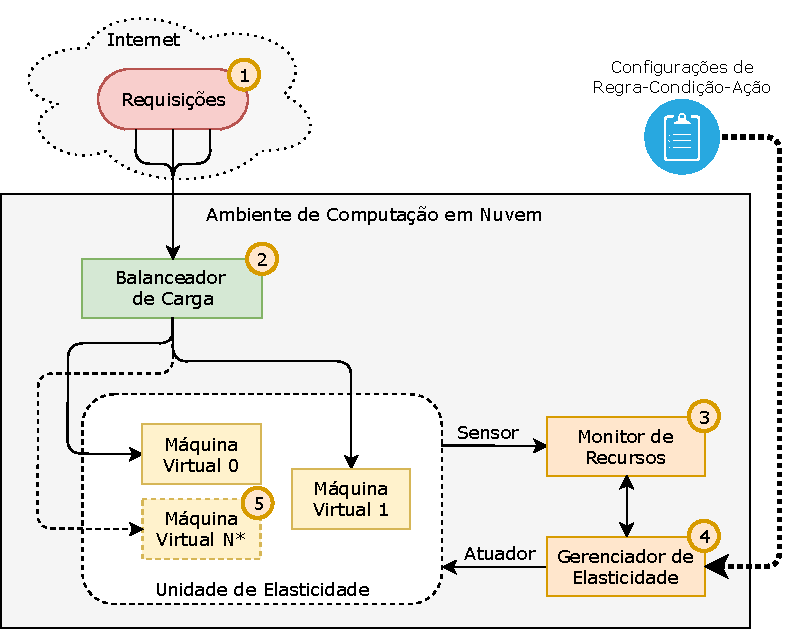
\includegraphics[width=\textwidth]{modelo-lb}
		\fonte{Elaborado pelo autor.}
%=======================================================================
%		EXPLICAMENTO
%=======================================================================
		\centering
		\begin{minipage}{.8\textwidth}
			\centering
			\small
			\vspace{1ex}
			\textbf{Fluxo de Execução:}
			\begin{enumerate}[leftmargin=*]
				\item Um número arbitrário de requisições são geradas na Internet;
				\item Dentro de um ambiente de computação em nuvem, um balanceador de carga absorve estas requisições e as distribui para um grupo de máquinas virtuais configuradas em uma unidade de elasticidade, tipicamente de maneira \textit{round-robin};
				\item Um serviço de monitoramento de recursos oferecido pelo provedor de computação em nuvem emite métricas de uso a respeito do consumo de recursos das máquinas virtuais;
				\item Através do gerenciador de elasticidade são executadas as tuplas do tipo \textquoteleft Regra~--~Condição~--~Ação\textquoteright, previamente configuradas pelo usuário e que determinam como a unidade de elasticidade deve reagir, seja adicionando ou removendo réplicas;
				\item No caso de excesso de demanda um conjunto de novas máquinas virtuais podem ser criadas, distribuindo a carga entre todas as disponíveis.
			\end{enumerate}
		\end{minipage}
%
	\end{minipage}
\end{figure}



%\chapter{Imagens Selecionadas do Modelo Elastipipe}




%=======================================================================
% Exemplo de Anexo
% O Anexo é utilizado para a ``inclusão de materiais não elaborados pelo
% próprio autor, como cópias de artigos, manuais, folders, balancetes, etc.
% e não precisam estar em conformidade com o modelo''.
%=======================================================================
%\annex
%\chapter{Artigos Publicados}
%Existe diferença entre os Apêndices e os Anexos.  Os apêndices trazem informação escrita pelo próprio autor do trabalho, incorporando-se ao formato da monografia como um todo.  Já um anexo é um material à parte, definido/publicado por si só, e que o autor julga conveniente ser apresentado juntamente com a monografia.  Normalmente também vai apresentar formato próprio, como um artigo publicado, um folder, uma planilha, etc.


\end{document}
